\documentclass[12pt]{book}
%\usepackage{natbib}
\usepackage[
	backend=bibtex,
	style=numeric,
]{biblatex}
\addbibresource{bibliographie}

\usepackage[utf8]{inputenc}

\usepackage[english]{babel}
\usepackage[T1]{fontenc}
\usepackage[a4paper,left=3cm,right=2.5cm,top=3cm,bottom=3cm, twoside]{geometry}
\usepackage{xcolor}
\usepackage{stmaryrd}
\usepackage{amssymb}
\usepackage{amsmath}
\usepackage{libertine}
\usepackage[pdftex]{graphicx}
\usepackage{caption}
\usepackage{subcaption}
\usepackage{float}
\usepackage{multirow}
\usepackage{apalike}
\usepackage{minitoc}
\usepackage{tikz}
\usepackage{enumitem}
\usepackage{epigraph}
%\usetikzlibrary{shadows.blur}
\usepackage{lscape}
\usepackage{titletoc}
%\usepackage{lipsum}
%\usepackage{cite}
\usepackage{booktabs}

\usepackage[nonumberlist]{glossaries}
\usepackage{calc}
\usepackage[]{titlesec} 
\definecolor{linkColor}{HTML}{32a852}
\usepackage[colorlinks=true,citecolor=linkColor,linkcolor=black]{hyperref}
\usepackage{fancyhdr}
\usepackage{lipsum}
\usepackage{spconf}
\usepackage{amsmath}
\usepackage{epsfig}
\usepackage{tabularx}
\usepackage{graphicx}
\usepackage{arydshln}
\usepackage{multirow}
\usepackage{bbding}
\usepackage{booktabs}
\usepackage{makecell}
\usepackage{amssymb}
\usepackage{hyperref}
\usepackage{Commands}
\usepackage{etoolbox} 
\usepackage{arydshln}
\setlength{\headsep}{20pt}
%%%%%%%%%%%%%%%%%%%%%%%%%%%%%%%%%%%%%%%%%%%%%%%%%%%%%%%%%%%%%%%%%%%%%%%%%%
%%%%%%%%%%%%%%%%%%%%%%%%%%%%%%%%%%%%%%%%%%%%%%%%%%%%%%%%%%%%%%%%%%%%%%%%%%
\setlength{\headheight}{15pt}

\definecolor{yourcolor}{HTML}{8a0e19}%{008bb2}

\titleformat{\chapter}[display]
{\normalfont\color{yourcolor}}
{\filleft\huge\color{black}\textsc\chaptertitlename\hspace*{2mm}%
	\begin{tikzpicture}[baseline={([yshift=-.6ex]current bounding box.center)}]
	\node[fill=yourcolor,circle,text=white] {\thechapter};
	\end{tikzpicture}
}
{1ex}
{\titlerule[1.5pt]\vspace*{1.5ex}\Huge\color{black}\textsc}
[]

\titleformat{name=\chapter,numberless}[display]
{\normalfont\color{black}}
{}
{1ex}
{\vspace*{-5cm}\Huge\textsc}
[]

%command to print the acutal minitoc
\newcommand{\printmyminitoc}[1]{%
	\noindent\hspace{1cm}%
	\colorlet{chpnumbercolor}{black}%
	\begin{tikzpicture}
	\node(s){
		\begin{minipage}{.9\linewidth}%minipage trick
		\printcontents[chapters]{}{1}{}
		\end{minipage}
	};
	{
		\color{yourcolor}
		\draw(s.north west)--(s.north east) (s.south west)--(s.south east);
	}
	\end{tikzpicture}
	\vspace*{3ex}
	
	#1
	\vfill
	\pagebreak
}


\newcommand{\HRule}{\rule{\linewidth}{0.7mm}}
\newcommand{\Hrule}{\rule{\linewidth}{0.3mm}}



%%%%%%%%%%%%%%%%%%%%%%%%%%%%%%%%%%%%%%%%%%%%%%%%%%%%%%%%%%%%%%%%%%%%%%%%%%%%%
%%%%%%%%%%%%%%%%%%%%%%%%%%%%%%%%%%%%%%%%%%%%%%%%%%%%%%%%%%%%%%%%%%%%%%%%%%





\begin{document}
	
	\begin{titlepage}
		\begin{center}
			\begin{tabular}{c@{\hskip 3cm}c}
				
\includegraphics[height=1cm]{images/UPC/logo-UPCite.jpeg} &
				
\includegraphics[height=1cm]{images/UPC/LIPADE.png}\\
			\end{tabular}
		\end{center}
	
		
		\begin{center}

			Université Paris Cité\\
			Laboratoire d’Informatique Paris Descartes (EA 2517)
  
  			\vfill
  			
	 		\HRule \\[0.1cm]
	 		 { \Large \bfseries     Exploration des synergies entre différentes tâches\\
        s'appuyant sur l'imagerie de télédétection multimodale\\
        et le texte pour un accès facilité à l'information	 }
	  		\Hrule \\
		
		\end{center}
		
		\vfill
			
		\begin{center}
			Presented by \textsc{\Large Hichem BOUSSAID}\\[1cm] 
			PhD thesis in \textsc{\large SPECIALTY}\\[1cm]
		
	
			
			\vspace{1cm}
	
			June 2021
		\end{center}
		
		\vspace{1cm}
			
		
		\begin{center}
			\begin{tabular}{lll}
				 \textsc{FULLNAME}  &  \textsc{Grade} & Reporter\\
				\textsc{FULLNAME}  &  \textsc{Grade} & Reporter \\
				\textsc{FULLNAME}  &  \textsc{Grade} & Supervisor\\
				\textsc{FULLNAME}  &  \textsc{Grade} & Supervisor \\
				
			\end{tabular}\\[1cm]
		\end{center}

	\newpage
	\end{titlepage}



\pagestyle{fancy}

\fancyhead{}

\renewcommand{\chaptermark}[1]{\markboth{\textsc{#1}}{}}



\frontmatter

\chapter*{Résumé}
\addcontentsline{toc}{chapter}{Résumé} 


Cette thèse est.

\chapter*{Abstract}
\addcontentsline{toc}{chapter}{Abstract} 

This work is.


\chapter*{Acknowledgments}
\startcontents[chapters]
\addcontentsline{toc}{chapter}{Acknowledgments}  


Merci.


% \begin{itemize}
%     \item Représentation spatiale linguistique: comment les humains utilisent les relations spatiales (motivation pour la partie B).
%     \item Représentation spatiale visuelle: comment les humains rapprochent visuellement des images (motivation pour la partie A)
% \end{itemize}


% \section{Thesis context}

% \textbf{Problematique / positionnement}

% Trouver 3-5 questions pour la thèse.


% \textbf{Verrous scientifiques}

% (?)


% \textbf{Organisation du document}


% \begin{itemize}
%     \item Tel ou tel partie, ces chapitres x,y,z, etc.
% \end{itemize}


\tableofcontents
\addcontentsline{toc}{chapter}{Table des matières}

\listoffigures
\addcontentsline{toc}{chapter}{Liste des figures}

\listoftables
\addcontentsline{toc}{chapter}{Liste des tableaux}

\chapter*{Preface}
\startcontents[chapters]
\addcontentsline{toc}{chapter}{Preface}  


\section*{Thesis context}

\begin{itemize}
    \item Présenter la thèse (qui, où, quoi, quand?)
\end{itemize}


\mainmatter

\setlength{\parskip}{.7em}

\titlespacing*{\section}{0pt}{.9em}{.8em}
\renewcommand{\baselinestretch}{1.1}


\fancyhead[RO]{\leftmark}
\fancyhead[LE]{\textsc{\chaptername~\thechapter}}


\part{Introduction}
% ============================================================
% CHAPTER 1: Introduction
% Expanded version: added a concrete vignette (1.1.2), a
% modality comparison table and real example-imagery figure
% (1.1.3), more depth in 1.1.1/1.1.4/1.1.5, and a thesis
% roadmap figure (1.1.7).
% ============================================================

\chapter{Introduction}
\label{chap:intro}

\startcontents[chapters]
\printmyminitoc{
\textit{Chapter summary.} Earth Observation satellites now acquire imagery at a volume, and a level of technical complexity, that exceeds what manual, expert-driven analysis can keep up with. This chapter traces this problem from its source (the sheer scale of acquisition) through the expertise barrier it creates, to natural language as an interface that can lower this barrier, along two complementary directions: answering questions about a known location, and retrieving locations that match a description. It closes by stating this thesis's research questions, scope, and the five contributions developed in Chapters~\ref{chap:llm_augmentation} through~\ref{chap:ctcr}.
}
% ============================================================

\section{Remote Sensing and Information Access}
\label{sec:intro_rs_access}
 
Every day, satellites orbiting the Earth acquire more imagery of its surface than any team of human analysts could examine in a lifetime. For the missions this thesis relies on, this imagery is free and openly available: a farmer, a disaster response coordinator, an environmental regulator can, in principle, download it themselves. In practice, almost none of them do, because turning a satellite image into an answer to a real question, is this field flooded, has this coastline eroded, requires a technical expertise that few of the people who need that answer actually have. This thesis is about closing that gap: not by producing more data, but by making the data that already exists accessible through natural language.
 
\section{The Remote Sensing Data Explosion}
\label{sec:intro_explosion}
 
Earth Observation satellites now acquire imagery of the Earth's surface systematically, repeatedly, and at global scale. This was not always the case. Earlier missions, such as the Landsat program, provided invaluable but comparatively sparse coverage: revisit times measured in weeks, moderate spatial resolution, and, for much of their history, data that was either commercially restricted or costly to access at scale. The Copernicus programme changed this. Sentinel-2 alone revisits every point on the Earth's land surface every five days, at up to 10\,m spatial resolution across 13 spectral bands~\cite{sentinel2}, while Sentinel-1 provides complementary all-weather radar coverage on a comparable revisit cycle~\cite{sentinel1}. Both are freely and openly available, without commercial licensing or access restrictions. This acquisition results in a continuously growing archive: over a decade of systematic global coverage now exists for the Sentinel missions alone, before accounting for the many other public and private satellite and airborne sensors in operation, and this volume continues to grow as new missions launch and existing archives extend.
 
This volume is, in one sense, an unprecedented asset: free, open, globally systematic imagery at a scale and consistency that did not exist a generation ago. In another sense, however, this same volume is the origin of the problem this thesis addresses. A scale of acquisition that has fundamentally outpaced the capacity of manual, expert-driven analysis is not simply more data to work with; it is a qualitatively different problem, one that data availability alone does not solve and, left unaddressed, actively worsens as the archive continues to grow.
 
\section{The Challenge of Information Extraction at Scale}
\label{sec:intro_extraction_challenge}
 
No team of trained analysts can visually inspect a meaningful fraction of what current EO missions acquire even in a single day, let alone sustain this indefinitely as the archive continues to grow. Scaling the number of analysts to match the scale of acquisition is not a viable solution: it is the interpretation step itself, not merely the volume of images to look at, that is the bottleneck.
 
Consider a concrete scenario. A disaster response coordinator, tasked with assessing flood extent after a storm, has access to newly acquired Sentinel-1 imagery of the affected region, chosen precisely because SAR penetrates the cloud cover that accompanies most flood events and typically blocks optical sensors. The imagery itself, however, does not show water; it shows radar backscatter, a measurement of surface roughness that the coordinator must learn to associate with flooding, while distinguishing it from other smooth surfaces (paved roads, bare soil) that produce a similar signal, and while accounting for terrain shadowing that can mimic or mask the same pattern. None of this is available on the image's surface: it requires training in SAR physics that a disaster response coordinator, however expert in their own domain, does not typically have. The same expertise gap recurs whenever a domain expert, rather than a remote sensing specialist, is the person best positioned to act on what the imagery reveals.
 
One might expect automation to close this gap on its own. Traditional remote sensing pipelines, built around scene classification, object detection, and semantic segmentation, do automate substantial parts of image interpretation, and are well established in the field. What they do not resolve is the gap this section is concerned with. Each of these pipelines is typically trained for one task, on one sensor, and transfers poorly to a different one, so a model trained to detect flooded roads offers little help answering a differently phrased question about the same imagery, or the same question on imagery from a different sensor. More fundamentally, their output remains low-level: a set of class labels, bounding boxes, or per-pixel masks, not an answer to the question a user actually has. Turning "this pixel is labeled water" into "yes, this area is flooded" is precisely the translation step a domain expert without remote sensing training cannot perform unaided, and that task-specific automation, however accurate at its own narrow task, does not perform for them either.

More generally, interpreting EO imagery correctly requires domain expertise that most potential users of this data do not have: knowing which spectral band combination reveals a given land cover type, correcting for atmospheric and radiometric effects, recognizing sensor-specific artifacts such as cloud shadows or radar speckle, and distinguishing genuine multi-temporal change from acquisition-condition variation. This expertise gap means that EO data, despite being open and freely available, remains inaccessible in practice to many of the people who would benefit most directly from it. Closing this gap, rather than simply producing more data, more analysts, or more task-specific automation, is the problem this thesis takes as its starting point.
 
\section{Towards Multimodal and Interactive Earth Observation}
\label{sec:intro_multimodal_interactive}
 
Addressing the expertise gap described above requires two things: sensing modalities rich enough to capture what an analyst would need to know, and an interface that does not itself require sensor-level expertise to use. This section introduces both, since they structure the remainder of this thesis.
 
\textbf{Sensing modalities.} EO sensors fall into two families, distinguished by how they acquire a signal. \textit{Passive sensors} record radiation already present in the scene, typically sunlight reflected off the Earth's surface; \textit{optical} and \textit{multispectral} sensors extend this beyond the visible range into bands such as the near-infrared that are informative for vegetation, water, and built surfaces but invisible to the human eye. Passive sensing requires daylight and is blocked by cloud cover. \textit{Active sensors} instead emit their own signal: \textit{Synthetic Aperture Radar} (SAR) emits microwave pulses and measures the backscattered amplitude and phase, a physical quantity, surface roughness and geometric structure, fundamentally different from reflectance, and the one at the center of the flood-mapping scenario above. Because SAR supplies its own illumination and operates at wavelengths that penetrate cloud cover, it acquires usable imagery day or night and in nearly all weather, complementing optical sensing rather than duplicating it.
 
These modalities also differ along resolution trade-offs that no single sensor can simultaneously optimize: \textit{spatial resolution} (the ground area per pixel), \textit{spectral resolution} (the number and specificity of wavelength bands recorded), and \textit{temporal resolution} (how frequently a location is reacquired, a prerequisite for detecting change). Three modalities spanning this trade-off recur throughout this thesis, summarized in Table~\ref{tab:intro_modalities}. Sentinel-2 is spectrally rich but spatially coarse. Sentinel-1 provides all-weather, day-or-night SAR coverage at a comparable spatial resolution to Sentinel-2, at the cost of a visual appearance considerably harder to interpret than optical imagery. Very High Resolution (VHR) aerial optical imagery, sourced in this thesis from the French national geographic institute's BD ORTHO product, offers spatial detail two to three orders of magnitude finer than either Sentinel mission, sufficient to resolve individual buildings and vehicles, but restricted in coverage to the regions it has been flown over and acquired far less frequently.
 
\begin{table}[ht]
\centering
\small
\caption{The three sensing modalities used throughout this thesis, spanning the spatial/spectral/temporal resolution trade-off introduced above.}
\label{tab:intro_modalities}
\begin{tabular}{lccc}
\toprule
& \textbf{VHR (BD ORTHO)} & \textbf{Sentinel-2 (MS)} & \textbf{Sentinel-1 (SAR)} \\
\midrule
Sensing type & Passive, optical & Passive, multispectral & Active, radar \\
Spatial resolution & $\sim$0.2\,m & 10--60\,m & $\sim$5\,m $\times$ 20\,m \\
Spectral bands & 3 (RGB) & 13 & 2 (VV/VH) \\
Coverage & France & Global & Global \\
Revisit time & 3 years & 5 days & 6 days \\
Weather/light dependent & Yes & Yes & No \\
\bottomrule
\end{tabular}
\end{table}
 
Figure~\ref{fig:intro_modality_example} shows two example locations imaged by all three modalities, with the VHR patch's extent marked within the wider multispectral and SAR context it sits inside. The contrast is immediately visible even to an untrained eye: the VHR image resolves individual buildings and vehicles within a small area; the Sentinel-2 composite shows the same location's broader surroundings at far coarser resolution but with additional spectral information; and the Sentinel-1 composite, dominated by speckle, encodes real information about surface structure that is not visually interpretable without training, precisely the barrier described in Section~\ref{sec:intro_extraction_challenge}. Combining these three modalities within a single model is consequently not a matter of stacking three images together: it requires reconciling different spatial resolutions and geographic extents, and different physical measurements (reflectance versus radar backscatter). Chapters~\ref{chap:tammi} and~\ref{chap:multitask} of this thesis address this combination directly, rather than treating multimodality as a minor implementation detail.
 
\begin{figure}[ht]
\centering
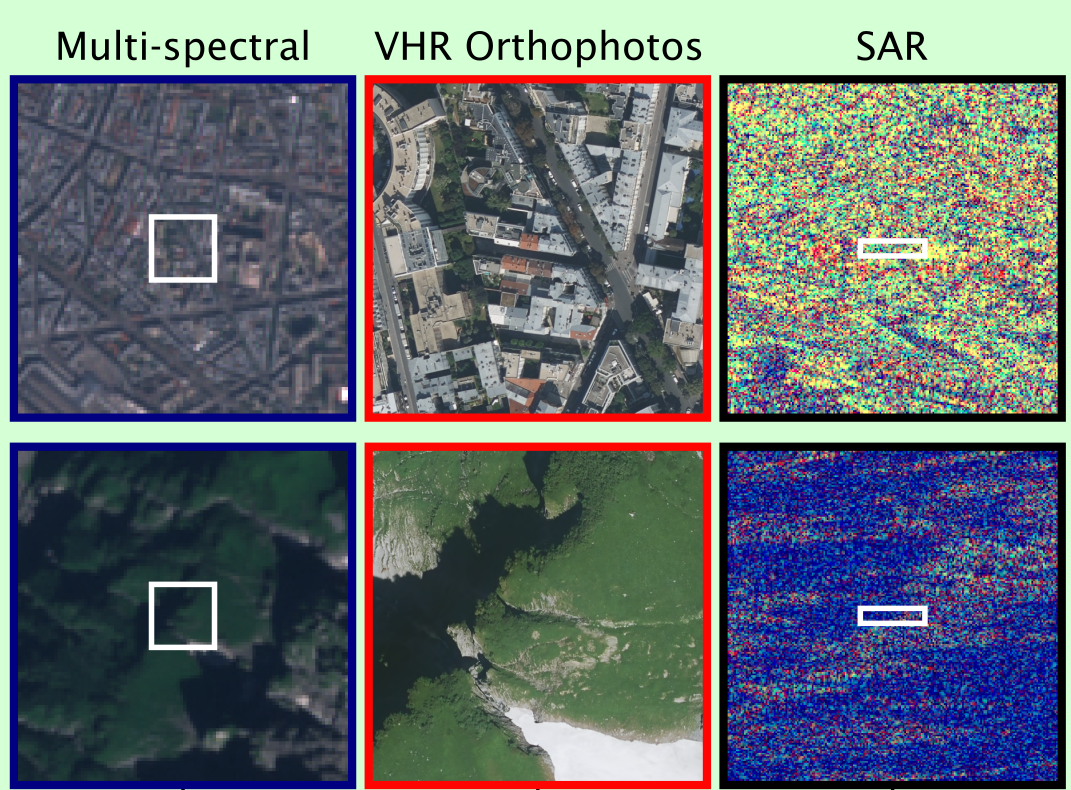
\includegraphics[width=0.85\textwidth]{images/introduction/tammi_graphabstract.png}
\caption{Two example locations imaged by the three modalities used throughout this thesis: Sentinel-2 multispectral, VHR optical (BD ORTHO), and Sentinel-1 SAR. The white rectangle marks the extent of the VHR patch within the wider spatial context covered by the multispectral and SAR imagery, illustrating the nested, multi-resolution relationship between the three modalities discussed below. Reflectance-based imagery (multispectral, VHR) is visually interpretable with some training; SAR backscatter is not, despite encoding genuine information about the scene. Figure from Chapter~\ref{chap:tammi}.}
\label{fig:intro_modality_example}
\end{figure}
 
\textbf{An interactive interface.} Richer sensing data alone does not close the expertise gap described in Section~\ref{sec:intro_extraction_challenge}; it can widen it, since more modalities and bands mean more, not less, specialized interpretation, as Figure~\ref{fig:intro_modality_example} illustrates directly. This thesis instead explores natural language as an interface that allows a user to interact with EO data directly in terms of what they want to know or find, without needing to manually locate, download, and visually interpret imagery themselves. This direction is not specific to remote sensing: it follows from the broader success, on natural images, of models that jointly learn from vision and language, closing part of the gap between a raw visual prediction and the semantic answer a user actually wants. Chapter~\ref{chap:relatedworks} reviews how this general direction has been adapted to remote sensing specifically; here, it is enough to note that three tasks recur throughout that adaptation, and structure this thesis. \textit{Captioning} produces a free-form natural-language description of an image. \textit{Visual question answering} (VQA) addresses the setting where the location of interest is already known: given an image and a question about it, produce an answer. \textit{Retrieval} addresses the inverse setting: given a description of what is being looked for, find the matching locations within a large archive. All three replace manual visual inspection, and the domain expertise it requires, with a natural language query or response; this thesis centers on VQA and retrieval specifically, with captioning appearing as a complementary training signal in Chapter~\ref{chap:multitask}.
 
\section{From Isolated Tasks to Unified Learning}
\label{sec:intro_isolated_unified}
 
RSVQA, the specific instantiation of question answering this thesis studies, has historically been developed as an isolated, single-modality task: a model trained to answer questions about one image, from one sensor, with no other training signal involved. This was, in part, a reasonable starting point: early RSVQA datasets were themselves single-modality, and studying one task on one modality kept the architectural and experimental design tractable while the field established basic feasibility. The first contributions of this thesis (Chapters~\ref{chap:llm_augmentation} and~\ref{chap:seg_attention}) work within this same single-modality setting, improving its robustness and its architecture respectively, before the thesis turns to two ways of moving beyond it.
 
The first is multimodality itself: an analyst's question is rarely answerable from a single sensor alone, as the flood-mapping scenario in Section~\ref{sec:intro_extraction_challenge} illustrates, motivating the combination of VHR, multispectral, and SAR imagery introduced in Section~\ref{sec:intro_multimodal_interactive} within a single RSVQA model (Chapter~\ref{chap:tammi}). The second is task combination: an analyst's needs often span more than question answering alone, encompassing description (captioning), and self-supervised reconstruction requires no annotation at all, only the imagery itself. A natural hypothesis is that training a model on several of these signals jointly, rather than in isolation, produces a shared representation more capable than any single-task model, through two distinct mechanisms: captioning can supply a richer, less templated supervisory signal than question-answering pairs alone, and self-supervised reconstruction can prevent that shared representation from collapsing onto purely semantic features, retaining visual detail a purely discriminative objective might otherwise discard. Whether this hypothesis holds is not, however, something this thesis assumes: Chapter~\ref{chap:multitask} treats it as an empirical question to be tested directly. Retrieval, the second paradigm introduced in Section~\ref{sec:intro_multimodal_interactive}, is not part of this task combination: Chapter~\ref{chap:ctcr} develops it separately.
\section{Scientific Challenges}
\label{sec:intro_challenges}
 
The progression described above, from single-modality RSVQA to multi-modal, multi-task, and retrieval settings, surfaces scientific challenges that structure the contributions of this thesis, and that Chapter~\ref{chap:relatedworks} situates in detail within the broader literature. These challenges fall into four related categories.
 
\textbf{Data-related challenges.} Multi-modal, richly annotated remote sensing datasets remain scarce relative to their natural-image counterparts, a scarcity compounded by the cost and expertise required to annotate imagery correctly, as Section~\ref{sec:intro_extraction_challenge} already established for human interpretation more broadly. Where datasets are generated automatically to work around this cost, as is common practice in RSVQA, the resulting questions are often templated, which risks introducing its own bias: a model can learn to exploit regularities in how questions are phrased rather than the underlying visual reasoning task, a robustness gap distinct from raw accuracy.
 
\textbf{Model-related challenges.} Adapting vision-language architectures developed for natural images to remote sensing is not a direct transfer. RSVQA architectures, for instance, typically compute attention directly from raw visual features, leaving them to jointly discover which regions of an image are relevant and what they mean from question-answering supervision alone, rather than exploiting the structured scene understanding that semantic segmentation already provides as an explicit, separately trainable signal. Handling heterogeneous modalities as different in resolution and physical meaning as VHR optical, multispectral, and SAR imagery, illustrated in Figure~\ref{fig:intro_modality_example}, compounds this further: a model must reconcile inputs that disagree in spatial extent, revisit frequency, and the underlying physical quantity they measure, which has not been systematically addressed at the dataset or architecture level.
 
\textbf{Learning challenges.} Beyond architecture, open questions remain about what a model should be trained to do, and with what supervision. Whether jointly training RSVQA with other tasks measurably improves performance, rather than degrading it, is assumed more often than it is tested; where it has been tested, results are mixed rather than confirmatory, leaving the actual value of multi-task training in this domain an open empirical question rather than a settled premise. Generalizing across sensors and geographic regions, and remaining robust to the kind of linguistic variation noted above, are further instances of the same underlying difficulty: learning representations that hold up outside the narrow conditions a model was trained under.
 
\textbf{Temporal and reasoning challenges.} Finally, most of the settings discussed so far concern a single image at a single point in time. Modeling temporal dynamics, and reasoning jointly over space, time, and language, is comparatively underexplored. Retrieving Earth Observation temporal imagery by composing a visual reference with a textual description of additional change has not previously been formulated as a task, despite its direct operational relevance to change monitoring, where an analyst who has already observed one change pattern often wants to find other locations exhibiting that same pattern together with something further.
 
\section{Research Questions and Thesis Scope}
\label{sec:intro_rq_scope}
 
The four categories of challenge described above raise a single overarching question that this thesis pursues throughout: how can multimodal, language-driven learning improve access to remote sensing information, by jointly leveraging vision and language, addressing data scarcity, exploiting synergies between tasks, and reasoning over space, time, and language together, rather than treating each of these as a separate concern. This thesis pursues that question through five specific research questions, each addressed by one of the contributions previewed in Section~\ref{sec:intro_contributions_overview}:
 
\begin{itemize}
\item \textbf{RQ1}: Can data-centric augmentation improve RSVQA models' robustness to linguistic variation in question phrasing, without sacrificing in-distribution accuracy?
\item \textbf{RQ2}: Does conditioning attention on an explicit semantic segmentation prior improve RSVQA over attention computed from raw visual features alone?
\item \textbf{RQ3}: How can RSVQA be extended to jointly exploit multiple sensing modalities acquired at different spatial resolutions?
\item \textbf{RQ4}: Does training RSVQA jointly with captioning and self-supervised image reconstruction measurably improve either task?
\item \textbf{RQ5}: Can a composed query, combining a visual reference and a textual description, support retrieval of temporal change patterns in Earth Observation archives?
\end{itemize}
 
The scope of this thesis follows directly from these questions. It addresses two language-based interfaces to EO data, question answering and retrieval, rather than the broader space of EO tasks, such as segmentation or detection as standalone goals, that this thesis does not address. The multi-modal and multi-task contributions (Chapters~\ref{chap:tammi} and~\ref{chap:multitask}) are developed and evaluated on datasets covering Metropolitan France, combining VHR, Sentinel-2, and Sentinel-1 imagery specifically; extending this scope geographically, or to further sensing modalities, is discussed as future work in the concluding chapter rather than undertaken here. 
\section{Thesis Contributions Overview}
\label{sec:intro_contributions_overview}
 
This thesis makes six technical contributions, developed across Chapters~\ref{chap:llm_augmentation} through~\ref{chap:ctcr}, each answering one of the five research questions stated in Section~\ref{sec:intro_rq_scope} and grouped into the three stages shown in Figure~\ref{fig:intro_roadmap}: single-modality RSVQA foundations, multi-modal and multi-task RSVQA, and retrieval as a complementary paradigm. Chapter~\ref{chap:relatedworks} first reviews the state of the art across visual question answering, retrieval, and captioning in remote sensing, positioning each contribution below relative to it.
 
\begin{figure}[ht]
\centering
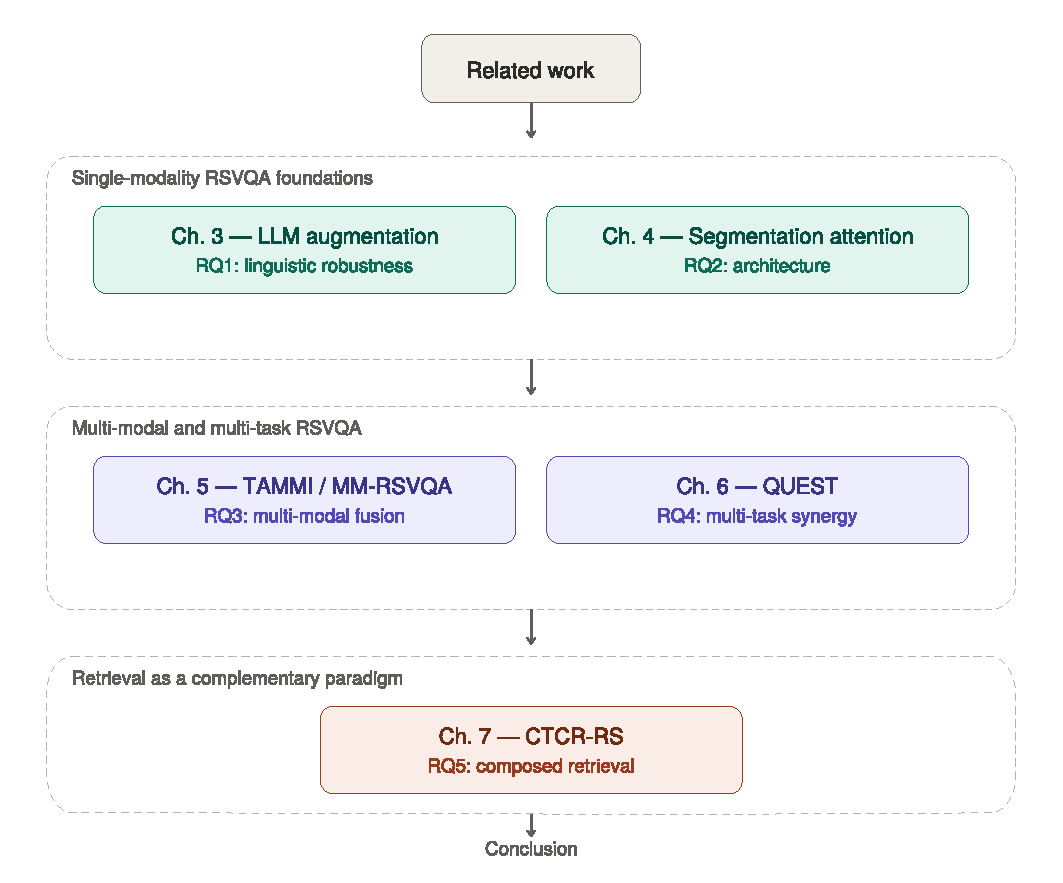
\includegraphics[width=0.85\textwidth]{images/introduction/thesis_roadmap.pdf}
\caption{Roadmap of this thesis's contributions, grouped into the three stages described in Section~\ref{sec:intro_contributions_overview}: single-modality RSVQA foundations (Chapters~\ref{chap:llm_augmentation}-\ref{chap:seg_attention}), multi-modal and multi-task RSVQA (Chapters~\ref{chap:tammi}-\ref{chap:multitask}), and retrieval as a complementary paradigm (Chapter~\ref{chap:ctcr}).}
\label{fig:intro_roadmap}
\end{figure}
 
\textbf{Chapter~\ref{chap:llm_augmentation}} answers RQ1, proposing an LLM-based data augmentation strategy that generates syntactically diverse reformulations of existing training questions, and showing that it improves robustness to unseen phrasings without sacrificing in-distribution accuracy.
 
\textbf{Chapter~\ref{chap:seg_attention}} answers RQ2, proposing a segmentation-guided attention mechanism that conditions the model's attention computation on an explicit, multi-channel semantic segmentation of the scene.
 
\textbf{Chapter~\ref{chap:tammi}} answers RQ3 through two contributions. It introduces TAMMI, a large-scale dataset combining VHR optical, Sentinel-2 multispectral, and Sentinel-1 SAR imagery, establishing multi-modal, multi-resolution VQA as a task in its own right; and MM-RSVQA, a baseline model that fuses all three modalities with the question.
 
\textbf{Chapter~\ref{chap:multitask}} answers RQ4, introducing QUEST, a unified architecture that jointly optimizes reconstruction, captioning, and VQA, and using it to test, rather than assume, whether joint training measurably improves either task.
 
\textbf{Chapter~\ref{chap:ctcr}} answers RQ5, introducing Composed Temporal Change Retrieval (CTCR-RS): given a reference pair of images depicting an observed change and a textual description of an additional change, retrieve archive locations exhibiting the composition of both.
 
The remainder of this thesis is organized as follows. Chapter~\ref{chap:relatedworks} reviews related work across RSVQA, retrieval, and captioning in remote sensing. Chapters~\ref{chap:llm_augmentation} through~\ref{chap:ctcr} present the six contributions summarized above, each structured with its own review of directly relevant related work, methodology, and experimental study. Chapter~\ref{chap:conclusion} concludes the thesis, synthesizing findings across all six contributions and discussing directions for future work.
 
\chapter{Related Works}
\epigraph{\itshape  A}{-- B}

\startcontents[chapters]
\printmyminitoc{
	%\lipsum[1]
}
% ============================================================
% CHAPTER 2, RELATED WORKS
% Structure: Introduction (with thesis roadmap) -> RSVQA (dense:
% Datasets, Methods) -> Retrieval (Datasets, Methods; CIR/COVR
% focus) -> Captioning (light: Datasets, Models) -> Task-agnostic
% foundation models (consolidated). Entries below match keys in
% related_works_refs.bib
% ============================================================

\section{Introduction}
\label{sec:rw-intro}

The volume of Earth Observation (EO) imagery acquired every day has grown far beyond the capacity of traditional, expert-driven analysis pipelines to exploit it. Natural language offers an accessible interface to this data, allowing non-expert users to query, describe, and search EO archives without specialized remote sensing knowledge. This idea has given rise to a family of vision-language tasks in remote sensing (RS): Visual Question Answering (RSVQA), which answers free-form questions about an image; cross-modal retrieval, which recovers imagery or text based on a query in the other modality; and image captioning, which generates a natural language description of a scene. More recently, these task-specific lines of work have started to converge into general-purpose RS vision-language models and foundation models, capable of handling several of these tasks, and others, within a single architecture.

This thesis engages with this landscape in two stages. It first focuses on RSVQA specifically, contributing three works that progressively extend RSVQA to new data augmentation strategies, segmentation-guided attention, and a new multi-modal dataset and model (TAMMI / MM-RSVQA) combining very high-resolution optical imagery with SAR and multispectral data. Building on this RSVQA foundation, the thesis then explores two directions that connect RSVQA to the other two tasks above: a composed temporal change retrieval contribution (CTCR-RS), which extends composed image retrieval to the temporal, multi-sensor setting; and a multi-task study that trains RSVQA jointly with image captioning and image reconstruction, examining the synergies between these three objectives within a shared model.

This chapter reviews the state of the art accordingly. Section~\ref{sec:rw-vqa} covers RSVQA in depth, the subject of the thesis' first three contributions. Section~\ref{sec:rw-retrieval} covers retrieval, focused on composed image retrieval (CIR), the family of methods CTCR-RS extends to the temporal setting. Section~\ref{sec:rw-captioning} covers captioning, focused on its use in conjunction with RSVQA, since captioning appears in this thesis as one component of the multi-task study rather than as an isolated contribution. Section~\ref{sec:rw-foundation} closes the chapter with task-agnostic RS vision-language models and foundation models, which increasingly cut across all three tasks above and are discussed separately rather than repeated in each task-specific section.

\section{Remote Sensing Visual Question Answering (RSVQA)}
\label{sec:rw-vqa}

\subsection{RSVQA datasets: modality, question diversity, and bias}
\label{sec:rw-vqa-datasets}

RSVQA was introduced by \textcite{lobry2020rsvqa} to allow users to query EO imagery through natural language questions such as "Is there a flood in this image?" or "How many buildings are in this area?". Since then, a large number of datasets have extended the task along three main axes: the image modality considered, the diversity and coverage of the questions, and the overall data volume.

\textbf{Modality of interest.} The image modality is a defining characteristic of a dataset, since it bounds the type of information the answers can be grounded in: optical imagery supports questions about roof color or crop type, multispectral imagery supports questions about vegetation health or water quality, and SAR supports questions about building height or flood extent. The large majority of existing datasets are optical-only, spanning several acquisition scales. UAV-based datasets such as FloodNet-v2~\cite{sarkar2023floodnet} and RescueNet~\cite{sarkar2023rescuenet} offer very fine resolution (0.015m) but limited spatial extent, aimed at post-disaster damage assessment. Satellite-based datasets such as RSVQA-LR~\cite{lobry2020rsvqa} trade resolution (10m, Sentinel-2) for broad, freely available coverage over the Netherlands. Aerial orthophoto datasets sit in between: RSVQA-HR~\cite{lobry2020rsvqa} (0.15m, USGS orthophotos over US cities) and CRSVQA~\cite{zhang2023crsvqa} (0.3m) support more localized, fine-grained questions than satellite data while remaining cheaper to acquire than UAV surveys. HRVQA~\cite{li2024hrvqa} and EarthVQA~\cite{wang2024earthvqa} sit at similarly high resolution (0.08m and 0.3m respectively), the latter specifically targeting relational reasoning over Chinese urban scenes (Nanjing, Changzhou, Wuhan). RSIVQA~\cite{zheng2021rsivqa} instead pools images from five heterogeneous existing datasets (UCM, AID, Sydney, DOTA, HRRSD) spanning 0.15-8m, prioritizing modality diversity over a single consistent acquisition source.

A smaller set of datasets move beyond single-modality optical imagery. CDVQA~\cite{yuan2022cdvqa} takes a bi-temporal image pair as input to support change-detection-style questions rather than static scene description. RSVQAxBEN-MM~\cite{tosato2024can} and OSVQA~\cite{zhao2024textguided} fuse optical and SAR imagery, and this thesis' TAMMI~\cite{boussaid2025tammi} extends this further with a richer multi-modal, multi-resolution design: very high-resolution optical imagery (0.2m, French National Geographic Institute) combined with 10-band multispectral and SAR (VV/VH/Ratio) data from Sentinel-1/2, spanning three distinct French regions (Paris and inner suburbs, Haute-Savoie, Hérault) chosen for urban, mountainous, and coastal diversity respectively. More recently, SAR-only datasets have emerged: SAR-VQA~\cite{cheng2025sartext} and SARLANG-1M~\cite{wei2025sarlang} focus exclusively on SAR imagery, aiming to advance the multi-modal understanding capabilities of instruction-tuned VLMs for SAR interpretation specifically, rather than SAR-optical fusion.

\textbf{Question diversity and coverage.} An ideal dataset would represent the full space of questions an end-user might ask. Fully manual annotation, as used for general-purpose VQA on natural images~\cite{lobry2020rsvqa}, remains rare at scale in RS due to its cost: FloodNet-v2 (43 unique questions), CRSVQA (674 unique questions), and RSIEval~\cite{hu2023rsgpt} (936 samples, purpose-built for evaluation rather than training) are the notable exceptions, but their scale limits the diversity they can offer. Most datasets instead derive questions automatically by filling predefined templates from existing labels or external geographic sources: RSVQA-HR derives questions from OpenStreetMap, while RSIVQA derives them from five source datasets' existing class labels. This approach necessarily bounds the achievable question diversity to what the source data covers; for instance, since OpenStreetMap does not track moving objects, no questions about cars can be generated from RSVQA-HR. TAMMI instead draws on multiple external geographic sources jointly (BD TOPO for geographic features, TRI for flood risk zones, BU20 for urban areas, CLC for land cover, EMA for mountain regions), which broadens the resulting question taxonomy to 21 distinct question types covering presence, quantity, location, classification, and relational analysis.

\textbf{Data volume.} Data volume is a joint consequence of the previous two axes and varies by several orders of magnitude: from a few hundred images (RSIEval) to hundreds of thousands of images and tens of millions of questions (RSVQAxBEN and RSVQAxBEN-MM~\cite{lobry2021rsvqaben,tosato2024can}, both derived from BigEarthNet). Some datasets ask a single question per image (e.g. GLVQA~\cite{GLVQA}), while most, including TAMMI, generate several questions per image, a choice that interacts directly with the answer-balancing strategy discussed below. RSSA~\cite{pang2024h2rsvlm} and VRSBench~\cite{li2024vrsbench} sit at an intermediate point, prioritizing broad visual coverage (1.4M and 29,614 images respectively) over per-image question density.

Table~\ref{tab:rw-vqa-datasets} summarizes the main characteristics of existing RSVQA datasets.

\begin{table}[h]
\centering
\small
\begin{tabularx}{\textwidth}{l X c c c}
\hline
\textbf{Name} & \textbf{Modalities} & \textbf{Resolution} & \textbf{\# Images} & \textbf{\# Questions} \\
\hline
TAMMI~\cite{boussaid2025tammi} & Optical (VHR), MS (10 channels), SAR (VV/VH/Ratio) & 0.2m / 10-20m & 282,852 & 3,162,514 \\
RSVQAxBEN-MM~\cite{tosato2024can} & Optical (RGB), SAR (VV/VH/Ratio) & 10m & 590,326 & 14,758,150 \\
OSVQA~\cite{zhao2024textguided} & Optical, SAR & 1/10m & 6,008 & 1,036,694 \\
RSVQAxBEN~\cite{lobry2021rsvqaben} & Optical (RGB) & 10m & 590,326 & 14,758,150 \\
Chessboard~\cite{tosato2025checkmate} & Optical (RGB) & 10m & 549,488 & 3,123,253 \\
RSIVQA~\cite{zheng2021rsivqa} & Various RGB & 0.15-8m & 37,264 & 111,134 \\
RSVQA LR~\cite{lobry2020rsvqa} & Optical (RGB) & 10m & 772 & 77,232 \\
RSVQA HR~\cite{lobry2020rsvqa} & Optical (RGB) & 0.15m & 10,659 & 1,066,316 \\
FloodNet-v2~\cite{sarkar2023floodnet} & UAV & 0.015m & 2,348 & 10,480 \\
RescueNet~\cite{sarkar2023rescuenet} & UAV & 0.015m & 4,375 & 65,328 \\
HRVQA~\cite{li2024hrvqa} & Optical (RGB) & 0.08m & 53,512 & 1,070,240 \\
EarthVQA~\cite{wang2024earthvqa} & Optical (RGB) & 0.3m & 6,000 & 208,593 \\
CDVQA~\cite{yuan2022cdvqa} & Bi-temporal RGB & 0.5/3m & 2,968 & \\
CRSVQA~\cite{zhang2023crsvqa} & Optical (RGB) & 0.3m & 4,639 & 4,644 \\
RSIEval~\cite{hu2023rsgpt} & Various RGB & & 100 & 936 \\
GLVQA~\cite{GLVQA} & USGS Ortho & 0.3m & 1'500 & 1'500  \\
RSSA~\cite{pang2024h2rsvlm} & Various RGB & 0.08/153m & 1,400,000 & 46,642 \\
VRSBench~\cite{li2024vrsbench} & Various RGB & & 29,614 & 52,472 \\
SAR-VQA~\cite{cheng2025sartext} & SAR & 0.5/15m & 130,000 & 130,000 \\
SARLANG-1M~\cite{wei2025sarlang} & SAR & 0.5/25m & 118,331 & 130,000 \\
\hline
\end{tabularx}
\caption{Existing RSVQA datasets, spanning UAV, aerial, and satellite acquisitions across optical, multispectral, and SAR modalities. Adapted and updated from \cite{boussaidtosato2025tour}.}
\label{tab:rw-vqa-datasets}
\end{table}

\textbf{Biases in RSVQA datasets.} RSVQA, like general-domain VQA, is prone to language bias: models can learn to exploit the skewed distribution of question-answer pairs rather than the image itself, for instance defaulting to "no" for presence questions because the geographic area covered is dominated by absence of the queried object. \textcite{chappuis2025langbias} study this systematically in RS and introduce the $LB_{score}$, which normalizes the prior answer distribution against the theoretical uniform distribution for a given question group, making bias comparable across question groups with very different answer-space sizes (e.g. binary yes/no questions versus open-ended counting questions). Dataset designers address this at the balancing stage of question generation, choosing between reflecting real-world answer distributions (introducing bias but preserving realism), enforcing complete balance (removing bias but also realism), or a compromise: \textcite{lobry2021rsvqaben} apply no balancing, while \textcite{tosato2025checkmate} cap each answer class at the count of its least-frequent class or its median value, and TAMMI applies different balancing rules depending on the answer type while capping the number of pairs per patch. A complementary mitigation strategy is to enforce a different question-answer distribution between training and test splits, e.g. by separating splits geographically (RSVQAxBEN~\cite{lobry2021rsvqaben}) or by drawing the test set from a distinct geographic region with different statistics (RSVQA-HR~\cite{lobry2020rsvqa}).

\subsection{Model architectures for RSVQA}
\label{sec:rw-vqa-methods}

RSVQA architectures typically decompose into four building blocks: image processing, question processing, multi-modal fusion, and answer prediction, as illustrated in Figure~\ref{fig:rw-vqa-pipeline}. This section reviews each in turn, then closes with training strategies that cut across all four. Models that address several of these building blocks at once as part of a larger, task-agnostic foundation model are discussed separately in Section~\ref{sec:rw-foundation}.
\begin{figure}[h]
\centering
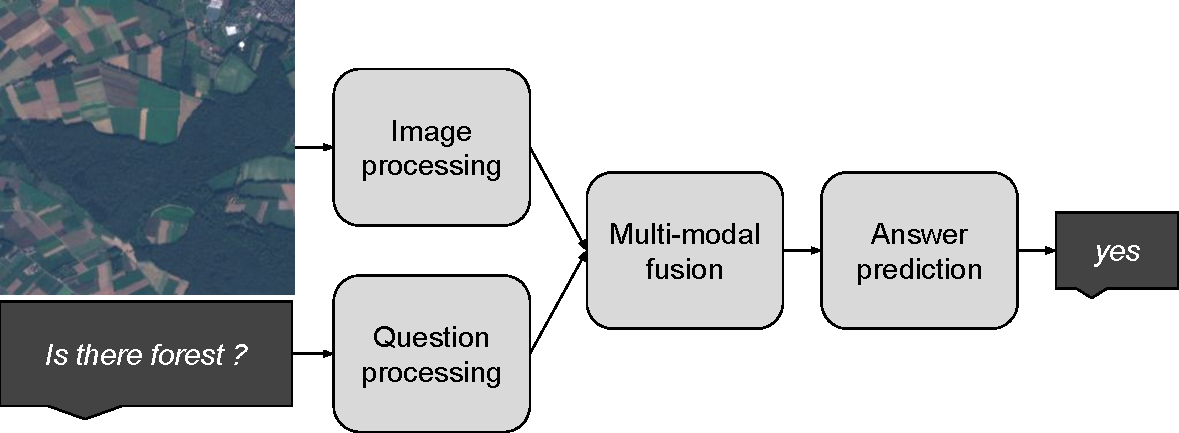
\includegraphics[width=0.85\textwidth]{images/relatedworks/RSVQAoverview.pdf}
\caption{The four building blocks of a typical RSVQA architecture: image and question are processed separately, combined through multi-modal fusion, and passed to answer prediction. Adapted from \cite{boussaidtosato2025tour}.}
\label{fig:rw-vqa-pipeline}
\end{figure}
 
\textbf{Image processing.} The RSVQA baseline~\cite{lobry2020rsvqa} extracts visual features with a frozen ResNet. Later work replaces this with transformer-based image encoders~\cite{bazi2022bimodal} or lightweight adapters that transfer a pretrained encoder's representations to the RSVQA-specific feature space at low cost~\cite{he2024pers}. Several architectures account for the multi-scale nature of RS scenes by explicitly modeling hierarchies across regions and objects, though they do so through different mechanisms: GLVQA~\cite{guo2022glvqa} captures global scene-level and local object-level visual information through two parallel branches whose outputs are fused before answer prediction; SHR-Net~\cite{zhang2023shrnet} instead performs explicit hierarchical spatial reasoning by progressively aggregating features across coarse-to-fine spatial scales; HMGR~\cite{zhang2024hmgr} encodes this hierarchy directly into a graph structure, discussed further under fusion below; SAMFPN~\cite{feng2024samfpn} adapts a feature-pyramid-network-style multi-scale representation combined with contextual attention; and CSCa~\cite{huang2024csca} adds a dedicated cross-modal semantic mapping module to align hierarchical visual features with the question representation. A distinct line of work injects object- or region-level structure directly: \textcite{felix2021crossmodal} use a dedicated object detector as feature extractor, while segmentation-guided attention~\cite{tosato2024segguided,wang2024earthvqanet} uses image segmentation to focus the model's attention on the regions relevant to the question. PAN-RSVQA~\cite{chappuis2025pan} combines several such pseudo-annotation streams (classification, segmentation, detection, generic features) from a vision foundation model into a single multi-task visual encoding. Beyond RGB, \textcite{tosato2025b} fuse optical and SAR features directly as visual input, establishing a baseline for SAR-aware RSVQA.

\textbf{Question processing.} This building block has received comparatively less attention. The baseline uses a Skip-thought RNN~\cite{kiros2015skipthought}; later work compares recurrent and transformer-based question encoders and studies whether to fine-tune them~\cite{chappuis2022a}, while masking irrelevant parts of the question during training has also been explored as a way to focus the model on question-relevant content~\cite{li2024maskbased}.

\textbf{Multi-modal fusion.} The baseline combines image and question representations via element-wise multiplication~\cite{lobry2020rsvqa}; \textcite{chappuis2021howtofind} systematically compare bi-modal fusion strategies and their computational cost. Cross-modal attention mechanisms are widely used to let one modality condition the other, though the direction and structure of that conditioning differs: the mutual attention inception network~\cite{zheng2021mutual} applies bidirectional attention (image-to-question and question-to-image) on top of an Inception-style visual backbone, \textcite{feng2023alternate} instead alternate the direction of attention guidance across training steps and combine this with a composite loss, and PERS~\cite{he2024pers} folds a lightweight cross-attention adapter directly into its parameter-efficient transfer mechanism. A second family adopts a full transformer as the fusion mechanism as the fusion mechanism itself, rather than a cross-attention layer added on top of otherwise separate encoders: \textcite{siebert2022multimodal} use a dedicated multi-modal fusion transformer that consumes modality-specific tokens, while \textcite{silva2022rsvqa} instead process concatenated image and question tokens through a single shared self-attention encoder, closer to a BERT-style joint encoder than to a two-stream cross-attention design. PAN-RSVQA~\cite{chappuis2025pan} uses a multi-modal transformer encoder over diverse image features and the question. A separate family shifts the balance toward language by first converting the image into a textual description and reasoning over both text streams jointly (Prompt-RSVQA and its extensions, discussed in Section~\ref{sec:rw-captioning-models} as they double as a captioning mechanism), while graph-based fusion represents multi-scale visual and multi-level linguistic features jointly in a shared semantic graph~\cite{zhang2024hmgr}.

\textbf{Answer prediction.} Most models frame answer prediction as classification over a fixed answer vocabulary, which is a natural fit for binary and multiple-choice questions but penalizes numerical answers indiscriminately: predicting "9" instead of "10" is scored identically to predicting "1000". To address this, several works add a regression head specifically for numerical answers~\cite{lobry2020rsvqa,blaga2024counting}, or predict numerical answers via direct text generation rather than classification~\cite{chappuis2023multitask}. Going further, a growing body of RS-adapted vision-language models generates free-form answers via auto-regressive decoding rather than selecting from a fixed vocabulary, discussed in Section~\ref{sec:rw-foundation}.

\textbf{Training strategies.} Beyond architecture, several works target the training procedure itself: curriculum learning that orders samples from easy to hard~\cite{yuan2022acurriculum}, dataset augmentation via language translation~\cite{yuan2023amultilingual}, momentum-distillation pseudo-labeling~\cite{li2024rsmodm}, adversarial training to reduce reliance on language bias~\cite{yuan2023badversarial}, and contrastive pretraining that aligns visual and linguistic representations before fusion~\cite{tian2024amvqa}.

\subsection{Evaluating RSVQA models}
\label{sec:rw-vqa-metrics}

RSVQA is most commonly evaluated with accuracy, but the specific form this takes varies. The baseline reports both an overall accuracy (pooling all questions together, which is dominated by the most frequent question types and answer classes) and an average accuracy across question types (weighting each question type equally, regardless of how many samples it contains), since the two can diverge substantially on an imbalanced dataset~\cite{lobry2020rsvqa}. For numerical questions specifically, plain classification accuracy treats all misclassifications as equally wrong, so regression-style metrics such as mean absolute error (MAE) and root mean squared error (RMSE) are reported alongside accuracy to capture how close a wrong answer actually was~\cite{lobry2020rsvqa}.

Accuracy alone, however, cannot distinguish a model that answers correctly by looking at the image from one that exploits language bias (Section~\ref{sec:rw-vqa-datasets}). To address this, \textcite{chappuis2025langbias} propose the relative accuracy metric, $RelAcc$, which rescales standard accuracy between a lower bound and an upper bound specific to each model and dataset:
\begin{equation}
RelAcc = \frac{Accuracy - LowerBound}{UpperBound - LowerBound} = \frac{Accuracy - AdversarialTesting}{100 - AdversarialTesting}
\end{equation}
The lower bound, $AdversarialTesting$, is obtained by taking the same trained model and testing it again at inference time, but with the image replaced by a tampered or missing one, using randomized, white-out, or black-out images (the authors show these three options give similar results). Answers the model still gets right in this setting are attributed to language bias rather than genuine visual grounding. The upper bound is taken as 100\%, or slightly less if the ground truth itself contains errors or unencoded answers. A model with a high standard accuracy but a $RelAcc$ close to 0\% is one whose predictions do not actually depend on the image, which accuracy alone would not reveal.

As RSVQA moves toward open-ended, generative answers (Section~\ref{sec:rw-foundation}) rather than classification over a fixed vocabulary, exact-match accuracy becomes increasingly unsuitable, since a semantically correct paraphrase would be scored as wrong. This has motivated the adoption of embedding-based text similarity metrics such as BERTScore~\cite{zhang2020bertscoreevaluatingtextgeneration}, which compares generated and reference answers using contextual token embeddings rather than surface-form overlap; this thesis' own evaluation methodology follows this direction for its multi-task study (Chapter~\ref{chap:multitask}), applying BERTScore to both VQA and captioning outputs, discussed further in Section~\ref{sec:rw-captioning-metrics}.

\subsection{Open challenges in RSVQA}
\label{sec:rw-vqa-challenges}

Four open challenges recur across the RSVQA literature and directly motivate part of this thesis' contributions. \textbf{Multi-modality}: while SAR and multispectral data are freely available and complementary to optical imagery, fusing them effectively remains harder than fusing multiple optical sources, since SAR-specific artifacts (speckle noise, geometric distortion) interact with the fusion mechanism in ways optical-only architectures do not anticipate~\cite{tosato2025b}; this thesis' TAMMI/MM-RSVQA contribution addresses this directly. \textbf{Answer space}: the classification-versus-generation tradeoff discussed under answer prediction above remains unresolved, with generative models offering more natural, open-ended answers at the cost of harder evaluation (Section~\ref{sec:rw-vqa-metrics}) and, as noted in Section~\ref{sec:rw-foundation}, frequently under-reported performance on numerical questions specifically. \textbf{Interpretability and explainability}: most architectures remain black boxes with respect to which image regions or reasoning steps produced a given answer; Checkmate~\cite{tosato2025checkmate} addresses this directly by identifying and pointing to the specific image regions supporting each answer, building on the segmentation and attention-based interpretability mechanisms discussed under image processing and fusion above. \textbf{Trustworthiness}: as discussed above, a model can achieve high accuracy while relying substantially on language bias rather than the image; $RelAcc$ provides a way to measure this, but mitigating it, rather than merely measuring it, remains largely open, with adversarial training~\cite{yuan2023badversarial} as one of the few dedicated attempts so far.

\section{Retrieval}
\label{sec:rw-retrieval}

\subsection{Retrieval datasets: from unimodal to composed and temporal}
\label{sec:rw-retrieval-datasets}

Cross-modal retrieval in RS is most commonly framed as image-text retrieval: given a textual query, retrieve the matching image(s) from an archive, or conversely. RSICD~\cite{lu2017exploring} and RSITMD~\cite{yuan2022exploring} are the standard benchmarks for this setting, repurposing captioning-style annotations and evaluating with recall@K metrics, while PatternNet~\cite{zhou2018patternnet} instead targets image-to-image retrieval based on visual similarity of scene patterns. This unimodal-query setting is well established and is not the focus of this section; CTCR-RS (Chapter~\ref{chap:ctcr}) instead sits within composed image retrieval (CIR), where the query combines an image and a text rather than a single modality.

CIR itself originates outside RS. In the general vision-language literature, CIRR~\cite{liu2021cirr} pairs 36,554 manually annotated triplets with 21,552 open-domain natural images sourced from NLVR2~\cite{NLVR2}, specifically designed to require reasoning about complex interactions between multiple objects in a scene rather than a single dominant object as in earlier, more constrained benchmarks; FashionIQ~\cite{wu2021fashioniq} instead targets a narrower, fashion-specific setting, with around 60,000 annotated triplets over roughly 77,000 product images across three clothing categories. Because manually annotating CIR triplets is costly, \textcite{ventura2024covr} propose CoVR, a scalable pipeline that automatically mines pairs of videos sharing a similar caption and uses a large language model to generate the corresponding modification text, yielding the 1.6-million-triplet WebVid-CoVR dataset; the same pipeline transfers directly to static images, and a CoVR-trained model achieves state-of-the-art zero-shot performance on CIRR and FashionIQ without ever seeing their manually annotated triplets. This automatic-triplet-mining idea, developed for natural images and video, is directly relevant to RS, where manual CIR annotation is at least as costly and no equivalent large-scale automatically mined resource yet exists.

PATTERNCOM~\cite{psomas2024composed}, built on top of PatternNet (38 classes, 800 images per class at 256$\times$256px), is the reference CIR dataset for RS. It covers eight attribute types (color, context, density, existence, quantity, shape, size, texture) over up to four classes each, with two to five values per class, yielding over 21,000 queries with between 2 and 1,345 positives per query, illustrated for each attribute type in Figure~\ref{fig:rw-patterncom-attrs}: a query image (e.g. a swimming pool) is paired with a text specifying a target attribute value (e.g. "kidney-shaped"), and the system must retrieve images of the same class exhibiting that attribute.
 
\begin{figure}[h]
\centering
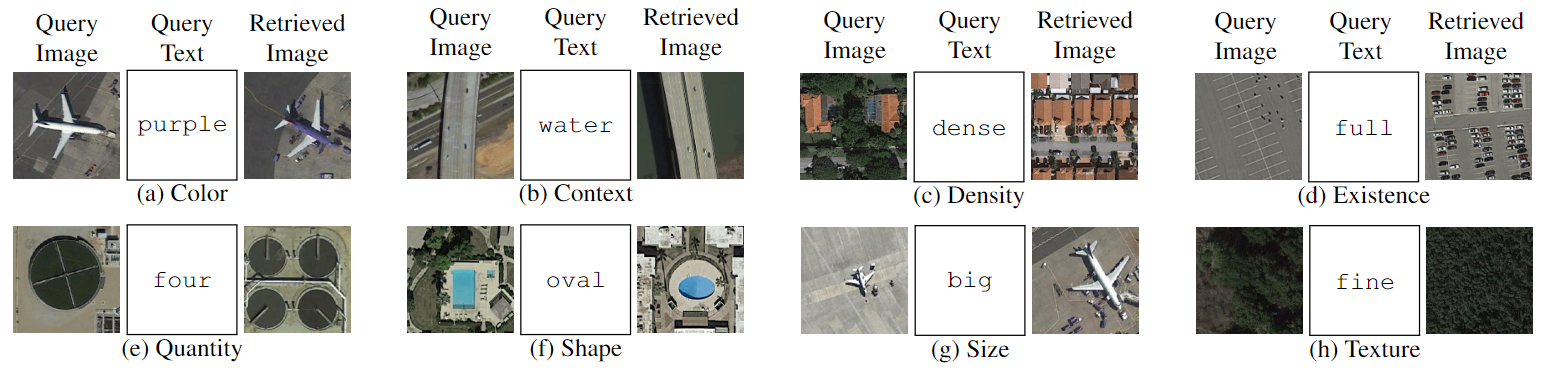
\includegraphics[width=\textwidth]{images/relatedworks/attr_use_cases_v2.png}
\caption{The eight attribute use cases covered by PATTERNCOM: color, context, density, existence, quantity, shape, size, and texture. Each query pairs a reference image with an attribute-modifying text and must retrieve an image of the same class exhibiting the target attribute value; subfigures (b) and (d) extend this to queries spanning multiple classes and attributes. Adapted from \cite{psomas2024composed}.}
\label{fig:rw-patterncom-attrs}
\end{figure}
 
Table~\ref{tab:rw-retrieval-datasets} summarizes the retrieval datasets and benchmarks discussed in this section, positioned along the unimodal-to-composed-to-temporal axis that leads to CTCR-RS.

\begin{table}[h]
\centering
\small
\begin{tabularx}{\textwidth}{l X c c}
\hline
\textbf{Name} & \textbf{Task / query type} & \textbf{Modalities} & \textbf{\# Images / pairs} \\
\hline
RSICD~\cite{lu2017exploring} & Image-text retrieval & Optical (RGB) & 10,921 \\
RSITMD~\cite{yuan2022exploring} & Image-text retrieval (fine-grained) & Optical (RGB) & 4,743 \\
PatternNet~\cite{zhou2018patternnet} & Image-image retrieval & Optical (RGB) & 30,400 \\
CIRR~\cite{liu2021cirr} & Composed image retrieval (natural images) & Optical (RGB) & 21,552 images, 36,554 triplets \\
FashionIQ~\cite{wu2021fashioniq} & Composed image retrieval (fashion) & Optical (RGB) & 77,684 images, 60,272 triplets \\
WebVid-CoVR~\cite{ventura2024covr} & Composed video retrieval, auto-mined & Video & 1.6M triplets \\
PATTERNCOM~\cite{psomas2024composed} & Composed image retrieval (image + text) & Optical (RGB) & 21,000+ queries \\
CTCR-RS (this thesis) & Composed temporal change retrieval (bi-temporal images + text) & Optical / SAR & 30,179 triplets \\
\hline
\end{tabularx}
\caption{Image-text, composed, and temporal retrieval datasets, from general-domain benchmarks (CIRR, FashionIQ, WebVid-CoVR) to remote sensing (RSICD, RSITMD, PatternNet, PATTERNCOM) and CTCR-RS.}
\label{tab:rw-retrieval-datasets}
\end{table}

\subsection{Methods for composed retrieval}
\label{sec:rw-retrieval-methods}

Outside RS, most CIR methods share a common architecture: a composition module fuses the reference image embedding and the modification text embedding into a single composed query embedding, which is then compared against candidate image embeddings via a contrastive objective, so that the composed embedding lands close to the target image and far from distractors. TIRG~\cite{vo2018composingtextimageimage} is an early example of this design, gating and residually combining image and text features rather than simply concatenating or averaging them. WEICOM, discussed next, departs from this paradigm entirely by avoiding a learned combiner altogether.

Composed image retrieval (CIR) was introduced to RS by \textcite{psomas2024composed} together with the PATTERNCOM benchmark above. Their method, WEICOM, is training-free: it fuses image-to-image and text-to-image similarities from a frozen VLM (CLIP or RemoteCLIP, discussed further in Section~\ref{sec:rw-foundation}) via a modality control parameter $\lambda$ that controls the relative weight given to the image and text parts of the query, avoiding the need for supervised composed-retrieval triplets that are costly to annotate at scale. This training-free design directly addresses the annotation bottleneck that motivated CoVR in the general vision-language literature, though via a different mechanism: WEICOM sidesteps the need for triplets altogether by fusing similarities at inference time, whereas CoVR sidesteps manual annotation by mining triplets automatically and still trains a dedicated combiner-style model. Follow-up work benchmarks composed retrieval specifically for applied EO use cases~\cite{efthymiadis2026benchmarking}, further establishing CIR as a distinct evaluation setting in RS beyond this initial benchmark.

PATTERNCOM's composed query, however, operates on a single, static image: the text modifies an attribute of a scene that does not itself change over time. This thesis' CTCR-RS contribution extends composed retrieval to the temporal setting: the reference is a bi-temporal image pair already exhibiting some change, and the text specifies an additional, compositional change to be added, with the target being a bi-temporal pair exhibiting the combined change. This is close in spirit to self-supervised cross-modal text-image time series retrieval~\cite{vuran2025selfsupervised}, which also moves retrieval toward multi-temporal image series, though without the compositional image-plus-text query structure that defines CIR. CTCR-RS can thus be read as the temporal, compositional counterpart to PATTERNCOM's attribute-based composed query, applied to the task of retrieving land-use and land-cover change rather than static scene attributes.

\subsection{Evaluating retrieval and composed retrieval}
\label{sec:rw-retrieval-metrics}

Retrieval, composed or otherwise, is evaluated with ranking metrics rather than classification accuracy, since the system returns a ranked list of candidates rather than a single answer. Recall@K (most commonly K = 1, 5, 10) reports the proportion of queries for which the correct target appears within the top-K retrieved candidates, and is the standard metric across RSICD, RSITMD, CIRR, FashionIQ, and PATTERNCOM alike. CIRR additionally reports a fine-grained Recall@K restricted to a small subset of visually similar distractors per query, specifically to prevent models from succeeding via coarse visual similarity alone rather than genuinely reasoning about the modification text. Mean or median rank of the correct target is sometimes reported alongside Recall@K, particularly when the candidate gallery is large enough that top-K recall alone saturates or fails to distinguish strong from weak retrieval quality. For CTCR-RS, the temporal, compositional nature of the query makes this distinction between coarse visual similarity and genuine change-reasoning especially relevant, echoing CIRR's fine-grained evaluation motivation above.

\subsection{Open challenges in composed retrieval}
\label{sec:rw-retrieval-challenges}

Composed retrieval in RS faces two open challenges directly relevant to this thesis. \textbf{Data scarcity}: unlike general-domain CIR, which benefits from automatically mined resources at the million-triplet scale (WebVid-CoVR~\cite{ventura2024covr}), RS composed retrieval still relies on a single, manually constructed benchmark (PATTERNCOM); no equivalent large-scale, automatically mined RS composed-retrieval resource yet exists, which likely limits how well WEICOM-style training-free methods and future learned combiners can be evaluated at scale. \textbf{Extending composition beyond static attributes}: PATTERNCOM's composed queries modify a single static attribute of a single-instant scene; extending composed retrieval to multi-temporal, multi-sensor settings, as CTCR-RS does, or to other forms of composition (e.g. compositional change across three or more time steps rather than two) remains largely unexplored.

\section{Captioning}
\label{sec:rw-captioning}

Image captioning is not a standalone contribution of this thesis; it appears as one component of a multi-task study alongside RSVQA and image reconstruction (Chapter~\ref{chap:multitask}). This section therefore does not survey RS captioning as a field in its own, but focuses on how captioning and RSVQA have been combined, either as a shared multi-task objective or as an intermediate mechanism within a VQA pipeline, since this is the angle relevant to the thesis' contribution.

\subsection{Datasets for joint captioning and RSVQA}
\label{sec:rw-captioning-datasets}

Datasets specifically built to support joint captioning-and-VQA study remain limited. RSICap~\cite{hu2023rsgpt} was introduced alongside RSGPT to provide long-form, detailed human-annotated captions suited to instruction-tuned VLMs, and is used by RSGPT for joint captioning and VQA fine-tuning. RS-Instructions, introduced alongside RS-LLaVA~\cite{diallo2024rsllava}, takes a different approach: rather than collecting new annotations, it combines four existing single-task captioning and VQA datasets (including UCM-Captions and RSVQA-LR) into a single multi-task instruction-tuning corpus. The underlying assumption is that joint training on this combined data improves general RS understanding more than task-specific fine-tuning would.

\subsection{Models coupling captioning and RSVQA}
\label{sec:rw-captioning-models}

Captioning and RSVQA have been coupled in the literature in two distinct ways. The first uses captioning-style image description as an interpretability step inside the VQA pipeline itself, rather than as an end task. Prompt-RSVQA~\cite{chappuis2022promptrsvqa} converts the image into a short textual description and feeds it, together with the question, to a language model, effectively delegating the visual grounding step to a captioning-like module before reasoning. MT-prompt-RSVQA~\cite{chappuis2023multitask} extends this by enriching the description with additional semantic information (land-cover classes, detected object counts) and by explicitly supervising an auxiliary counting objective, optimized jointly with the main VQA loss during training rather than handled by a separate, frozen pipeline step. PAN-RSVQA~\cite{chappuis2025pan} generalizes the idea further, using a vision foundation model to produce several pseudo-annotations (classification, segmentation, detection, generic features) jointly consumed by a multi-modal transformer; the visual description function that a captioning model would otherwise fill is here distributed across several pseudo-annotation streams.

The second family treats captioning and VQA as two supervised outputs of a single shared model, trained jointly on blended datasets rather than one task feeding the other. RS-LLaVA~\cite{diallo2024rsllava} adapts LLaVA to RS imagery via LoRA fine-tuning on the RS-Instructions dataset described above. In a related but architecturally different setting, a UAV aerial video model~\cite{uav2024videocaptioning} explicitly chains the two tasks, inserting a VQA step before the captioning decoder so that the answers to solicited questions enrich the information available for caption generation, an ordering that is the mirror image of Prompt-RSVQA's caption-then-answer pipeline.

These two families illustrate the two ways captioning and VQA have been coupled in the literature: captioning (or a captioning-like description) as an intermediate representation feeding VQA reasoning (Prompt-RSVQA, MT-prompt-RSVQA, PAN-RSVQA), and captioning and VQA as jointly supervised, parallel outputs of a shared model (RS-LLaVA, the UAV video model). The multi-task study in Chapter~\ref{chap:multitask} sits closer to the second family, but adds image reconstruction as a third, self-supervised objective alongside VQA and captioning, which neither of the above considers. Larger, task-agnostic VLMs that also cover captioning and VQA among several other capabilities (e.g. RSGPT, GeoChat) are discussed in Section~\ref{sec:rw-foundation}.

\subsection{Evaluating captioning alongside RSVQA}
\label{sec:rw-captioning-metrics}

Captioning is conventionally evaluated with n-gram overlap metrics borrowed from machine translation and general-domain captioning: BLEU measures precision of overlapping n-grams against reference captions, ROUGE measures recall-oriented overlap, and METEOR additionally accounts for synonymy and stemming; CIDEr, designed specifically for captioning, weights n-grams by their TF-IDF specificity so that generic, uninformative phrases contribute less to the score than distinctive ones. All four remain standard on NWPU-Captions, RSICD, and related benchmarks. These metrics, however, rely on surface-form overlap with a fixed set of reference captions and penalize a semantically correct but differently-worded caption. As discussed for VQA (Section~\ref{sec:rw-vqa-metrics}), this thesis' evaluation methodology adopts BERTScore~\cite{zhang2020bertscoreevaluatingtextgeneration} for its multi-task study, applying the same embedding-based similarity metric to both the captioning and VQA outputs of the shared model, which allows a single evaluation methodology to cover both tasks, reported alongside accuracy for VQA and ROUGE-1/ROUGE-L for captioning.

\subsection{Open challenges in joint captioning and RSVQA}
\label{sec:rw-captioning-challenges}

The main open challenge specific to the captioning-and-VQA setting reviewed in this section is that joint training is consistently motivated by an assumed synergy between tasks, but that synergy is rarely measured directly, and where it is measured, the evidence is mixed rather than confirmatory: RS-LLaVA's own reported results show single-task fine-tuning outperforming joint training on both captioning and VQA metrics, directly contradicting the premise behind combining the two tasks in RS-Instructions. Prompt-RSVQA-style approaches treat a captioning-like description as beneficial to VQA reasoning by construction, but in each case the improvement is attributed to the combination as a whole rather than isolated per task: it remains unclear how much of the gain comes specifically from captioning, how much from VQA, and how the two interact when a third objective is added. This thesis' multi-task study (Chapter~\ref{chap:multitask}) addresses this directly by ablating each task, training RSVQA, captioning, and image reconstruction jointly, to measure the specific contribution of each task to the others rather than assuming it. A related, more general challenge is the tension between the short, template-derived captions typical of automatically generated RS captioning data and the longer, richer descriptions that better support a VQA-style reasoning objective when the two tasks are trained jointly; datasets such as RSICap that provide long-form, human-written captions specifically for instruction-tuned VLMs are one response to this tension, but at the cost of scale relative to automatically annotated alternatives.
\section{Task-agnostic models and foundation models}
\label{sec:rw-foundation}

The families reviewed above are largely task-specific: an architecture designed for RSVQA, for CIR, or for captioning. A separate and increasingly dominant line of work instead builds a single RS-adapted model intended to handle several of these tasks at once, typically by adapting a pretrained large language model (LLM) or contrastive vision-language model to RS imagery. This section reviews these task-agnostic models, split into instruction-tuned generative VLMs and contrastive foundation encoders.

\textbf{Instruction-tuned generative VLMs.} RSGPT~\cite{hu2023rsgpt} fine-tunes an LLM-based VLM specifically for RS image understanding using the RSICap dataset (Section~\ref{sec:rw-captioning-datasets}), reporting gains on both captioning and VQA from joint instruction tuning. GeoChat~\cite{kuckreja2024geochat} extends this to grounded, region-level question answering. LHRS-Bot~\cite{muhtar2025lhrsbot} and its improved successor LHRS-Bot-Nova incorporate volunteered geographic information to strengthen visual-linguistic grounding, while SkyEyeGPT~\cite{zhan2025skyeyegpt} unifies several RS vision-language tasks, including VQA, through instruction tuning. EarthGPT~\cite{zhang2024earthgpt} processes SAR, optical, and infrared inputs jointly through a cross-modal comprehension module, extending capability beyond optical imagery within a single unified model.

More recent unified models push further toward multi-task, multi-sensor coverage: SkySenseGPT~\cite{luo2024skysensegptfinegrainedinstructiontuning} builds on the SkySense foundation model with fine-grained instruction tuning for vision-language understanding, RSUniVLM~\cite{liu2024rsunivlmunifiedvisionlanguage} and GeoRSMLLM~\cite{zhang2025georsmllmmultimodallargelanguage} adopt mixture-of-experts or unified architectures spanning multiple granularities of RS vision-language tasks, and TEOChat~\cite{irvin2025teochatlargevisionlanguageassistant} and UniRS~\cite{li2024unirsunifyingmultitemporalremote} specifically target temporal RS data, extending question answering to multi-temporal image series rather than single acquisitions. This temporal extension is directly relevant to the composed temporal retrieval setting this thesis addresses in Chapter~\ref{chap:ctcr}, even though these models target question answering rather than retrieval. A recurring limitation across this family, already noted in the RSVQA literature specifically~\cite{boussaidtosato2025tour}, is that most of these generative VLMs report strong results on descriptive or classification-style questions but rarely publish detailed results on the numerical questions that RSVQA datasets, which limits fair comparison against the task-specific classification-based baselines discussed in Section~\ref{sec:rw-vqa-methods}.

\textbf{Contrastive foundation encoders.} A separate, encoder-only line of work adapts CLIP-style contrastive pretraining to RS imagery, producing a general-purpose visual-textual embedding space rather than a generative decoder. RemoteCLIP~\cite{liu2024remoteclip} is the reference model in this family and is used directly as the frozen encoder backbone in WEICOM (Section~\ref{sec:rw-retrieval-methods}). RS5M and GeoRSCLIP~\cite{zhang2024rs5m} scale this pretraining to a larger RS image-text corpus, and more recent encoders such as DGTRS-CLIP~\cite{chen2025dgtrsddgtrsclipdualgranularity}, which targets dual-granularity alignment, continue this line of work. All of these report unimodal image-text retrieval performance as a core evaluation of alignment quality, and any of them could in principle serve as the frozen encoder backbone for a WEICOM-style composed retrieval method, though to date only CLIP and RemoteCLIP have been evaluated in that specific composed setting. Because these encoders are trained without any task-specific supervision, they are equally applicable to retrieval, zero-shot classification, and as a visual encoder for VQA or captioning models, making them the clearest instance of the task-agnostic framing that motivates this section.

\section{Positioning of this thesis}
\label{sec:rw-positioning}
 
The landscape reviewed in this chapter is where this thesis' five contributions fit. The first three sit within RSVQA specifically (Section~\ref{sec:rw-vqa}). A data augmentation strategy targets the training-strategy dimension reviewed in Section~\ref{sec:rw-vqa-methods}. Segmentation-guided attention uses image segmentation to focus the model's attention on question-relevant regions, one of the interpretability mechanisms discussed under image processing in Section~\ref{sec:rw-vqa-methods}. TAMMI/MM-RSVQA addresses the multi-modality challenge identified in Section~\ref{sec:rw-vqa-challenges} directly, by fusing very high-resolution optical imagery with SAR and multispectral data rather than optical imagery alone.

The remaining two contributions extend this RSVQA foundation outward, each into one of the other two tasks reviewed in this chapter. Unlike PATTERNCOM, which relies on manual triplet annotation, CTCR-RS is built by extracting change labels automatically from existing change captinoing datasets, closer to the automatic-construction of CoVR than to PATTERNCOM's manual annotation, even though the underlying mechanism differs. No prior RS dataset or method extends composition beyond static attributes to compositional, multi-temporal change. The multi-task study (Section~\ref{sec:rw-captioning}) instead connects RSVQA to two other tasks in a different way, training RSVQA jointly with captioning and image reconstruction and directly addressing the open challenge identified in Section~\ref{sec:rw-captioning-challenges}: rather than assuming a synergy between jointly trained tasks that goes unmeasured, or, as in RS-LLaVA's own results, contradicted, it isolates the contribution of each task through systematic ablation across every task combination.
 
This progression is not a coincidence: RS vision-language research began with  task-specific architectures for RSVQA, captioning, and retrieval studied largely in isolation, and is increasingly moving toward models and methods that treat these tasks, and the synergies between them, together rather than as three separate problems (Section~\ref{sec:rw-foundation}). The remaining chapters detail each of the five contributions in turn.
%\chapter{Contributions}
\label{chap:contributions}
 
\section{Scientific Objectives}
\begin{itemize}[leftmargin=1.5em]
    \item Improve RSVQA through better architecture and data strategies
    \item Build a multimodal multi-resolution benchmark for RS
    \item Leverage LLMs to enhance data diversity and model generalization
    \item Explore task synergies between QA and Captioning
    \item Address change-aware information retrieval in RS
\end{itemize}
 
\section{Document Outline}
    Diagram or table linking each contribution to the corresponding chapter.


%\part{Remote Sensing Visual Question Answering}

\chapter{LLM-Driven Data Augmentation for Visual Question Answering}
\epigraph{\itshape  La volonté trouve, la liberté choisit. Trouver et choisir, c'est penser}{-- Victor Hugo}

\startcontents[chapters]
\printmyminitoc{
	%\lipsum[1]
}


%\def\BibTeX{{\rm B\kern-.05em{\sc i\kern-.025em b}\kern-.08em
    %T\kern-.1667em\lower.7ex\hbox{E}\kern-.125emX}}

%\title{LLM Augmentation for Robust RSVQA}
%\title{LLM-Driven Data Augmentation for Visual Question Answering}



%\author{\IEEEauthorblockN{Hichem Boussaid, Nayoung Kwon, Camille Kurtz, Laurent Wendling, Sylvain Lobry}
%\IEEEauthorblockA{\textit{LIPADE, Université Paris Cité, 75006 Paris, France}}
%firstname.lastname@u-paris.fr}

%\maketitle

%\ck{le titre est vraiment trop proche du papier concurrent : Multilingual Augmentation for Robust Visual Question Answering in Remote Sensing Images}

%\ck{Quelques articles récents pour compléter ton SOA : https://www.sciencedirect.com/science/article/pii/S1077314223002424

%https://www.ecva.net/papers/eccv_2022/papers_ECCV/papers/136960094.pdf

%https://aclanthology.org/2024.eacl-srw.20.pdf

% et un survey
%https://export.arxiv.org/pdf/2401.15422
%https://github.com/MLGroup-JLU/LLM-data-aug-survey
%}
\section{Introduction}
\label{sec:chap3_intro}
% ============================================================
 
Despite growing interest in RSVQA, a fundamental limitation
persists across existing approaches: poor generalization to unseen
question formulations. Most RSVQA datasets are automatically
generated from geospatial vectorial databases such as OpenStreetMap~\cite{openstreetmap}\cite{lobry2020rsvqa},
which results in a limited set of question
templates. Models trained on such data learn to exploit
surface-level linguistic patterns rather than developing a robust
understanding of the underlying visual content. As a
consequence, even semantically equivalent questions,
differing only in wording or syntactic structure, can lead to
dramatically different model predictions. This phenomenon,
known as linguistic bias, has been identified as a critical
obstacle to the deployment of RSVQA systems in real-world
scenarios where users formulate queries freely and
unpredictably~\cite{chappuis2023curse}.
 
It is worth noting that this work was conducted at a time when
RSVQA models predominantly relied on a dual-encoder
architecture, a visual encoder such as ResNet~\cite{he2015deepresiduallearningimage} or a Vision
Transformer~\cite{dosovitskiy2021imageworth16x16words})
paired with a text encoder such as BERT~\cite{sanh2020distilbertdistilledversionbert},
 followed by a fusion module for answer prediction. In this
paradigm, the model has no generative capacity and no world
knowledge beyond what is encoded in its training data, making
it particularly sensitive to the linguistic distribution of the
training questions. The recent shift toward large
vision-language models with generative capabilities has
partially alleviated this problem by leveraging pre-training on
massive and diverse corpora. However, at the time of this
work, such models were not yet established in the remote
sensing domain, and the challenge of linguistic generalization
in RSVQA remained largely unaddressed. The contribution
presented in this chapter should therefore be understood in
this context: a targeted, data-centric approach to improve
robustness within the then-dominant encoder-based RSVQA
framework.
 
Data augmentation is a natural strategy to address this
limitation. Two approaches have been widely studied in the
natural language processing literature: paraphrasing and back
translation. Paraphrasing involves rewriting a sentence while
preserving its meaning, but rule-based methods often fail to
capture the full range of linguistic variation and do not scale
to large datasets~\cite{bhagat2013paraphrase}. Back
translation, translating a question into an intermediate
language and then back into the original, offers a scalable
alternative~\cite{yuan2023multilingual}. However, it tends to
produce questions that remain structurally close to the
original, limiting the diversity of the augmented dataset.
Furthermore, translation quality varies depending on the
language pair and domain vocabulary, which can introduce
noise into the training data.
 
The emergence of Large Language Models (LLMs) offers a
fundamentally new perspective on this problem. Models such
as LLaMA-2~\cite{touvron2023llama2openfoundation}, trained on massive
corpora with instruction-following capabilities, can generate
diverse, coherent, and semantically faithful reformulations of
a given question with minimal supervision. Unlike back
translation, LLM-based paraphrasing is not constrained by the
structure of a pivot language and can produce syntactically
varied outputs while preserving the semantic content and
expected answer. This makes LLMs particularly well-suited
for the RSVQA augmentation problem, where the goal is to
expose the model to a wide variety of question formulations
without altering the ground truth.
 
In this chapter, we propose a data augmentation framework
based on LLMs to improve the robustness and generalization
of RSVQA models. Concretely, we use LLaMA-2-7B to
generate ten semantically equivalent reformulations of each
question in the RSVQA-HR dataset~\cite{lobry2020rsvqa},
guided by a prompt selected through systematic evaluation of
nine candidates across questions of varying linguistic
complexity. We compare this approach against back translation
and evaluate both in terms of in-distribution performance and
generalization to unseen question formulations.
 
The remainder of this chapter is organized as follows.
Section~\ref{sec:chap3_rw} reviews related work on data
augmentation for VQA and the use of LLMs for text
generation. Section~\ref{sec:chap3_method} presents the
proposed augmentation methodology.
Section~\ref{sec:chap3_experiments} details the experimental
setup and results. Section~\ref{sec:chap3_conclusion} concludes
the chapter and discusses limitations and perspectives.

\section{Related Work}
\label{sec:chap3_rw}

\subsection{Data Augmentation in Natural Language Processing}
\label{sec:chap3_rw_nlp}
 
Data augmentation in NLP aims to increase training data
diversity without new annotations, improving model
robustness and reducing overfitting. Early work focused
on simple rule-based token-level operations.
\cite{wei2019eda} proposed Easy Data Augmentation (EDA),
consisting of four lightweight operations: synonym
replacement, random insertion, random swap, and random
deletion, that improved performance on text
classification tasks, especially in low-resource settings.
Despite their simplicity, these operations suffer from a
fundamental limitation: modifications are local and may
introduce semantic inconsistencies for complex or
domain-specific sentences. In the RSVQA context, where
questions involve spatial relations and domain vocabulary
(\textit{e.g.}, \textit{``at the bottom of a rectangular
commercial building''}), such perturbations can 
corrupt the intended meaning entirely.
 
Back translation, originally proposed by
\cite{sennrich2016backtranslation} for neural machine
translation, offers a more principled alternative: a
source sentence is translated into a pivot language and
then back into the original, yielding a paraphrase that
preserves meaning while introducing new surface forms.
\cite{edunov2018backtranslation} later studied this
approach at scale, confirming its benefits across
generation tasks. However, back translation is
constrained by the quality of the underlying translation
system and tends to produce output that remains
structurally close to the original, as the pivot language
acts as a bottleneck on syntactic diversity. For questions
involving rare or domain-specific terms, translation
quality degrades further, potentially introducing noise
into training data.
 
\subsection{Data Augmentation for VQA and RSVQA}
\label{sec:chap3_rw_vqa}
 
Language bias is a well-documented problem in VQA: models
trained on datasets with skewed answer distributions
learn to exploit statistical shortcuts in questions rather
than performing genuine visual reasoning. Data augmentation
has emerged as a primary strategy to mitigate this.
\cite{gokhale2020seada} introduce Semantic Equivalent
Adversarial Data Augmentation (SEADA), generating
adversarial question paraphrases using syntactically
controlled paraphrase networks, showing improved VQA
robustness to linguistic variation.
\cite{sheng2021contrastclassify} propose a contrastive
training objective that explicitly encourages VQA
representations to be invariant to question rephrasing,
achieving gains on the VQA-Rephrasings benchmark which
evaluates answer consistency across human-written
paraphrases. \cite{chen2022rethinkingDA} propose KDDAug,
a knowledge distillation-based augmentation framework
that generates new image-question pairs and assigns
pseudo-answers via a teacher model, improving robustness
across question types without human-designed rules.
 
In the remote sensing domain specifically, the
generalization problem is more severe than in standard
VQA. \cite{chappuis2023curse} provide a systematic
analysis through visual-blind models and adversarial
testing, showing that RSVQA models rely heavily on
linguistic shortcuts and that biases stem from the
automatic and template-based question generation
strategies used in existing RS datasets.
\cite{yuan2023adversarial} address this from the model
side, introducing an adversarial training framework with
regularizers to reduce language bias in RSVQA.
The most directly related augmentation work is that of
\cite{yuan2023multilingual}, who apply back translation
to RSVQA questions via Chinese, German, and French as
pivot languages, combined with a contrastive learning
strategy to train more robust representations. While
effective, this approach is limited by the structural
proximity of back-translated questions to their originals
and by translation quality degradation on RS-specific
vocabulary. The work presented in this chapter directly
addresses these limitations by replacing back translation
with LLM-driven generation, which produces more
syntactically diverse reformulations while maintaining
semantic fidelity.
 
\subsection{Large Language Models for Paraphrasing and Question Generation}
\label{sec:chap3_rw_llm}
 
The use of LLMs for controlled paraphrasing and text
generation has grown rapidly with instruction-tuned
models. Unlike back translation, LLM-based paraphrasing
is not constrained by a pivot language and can be guided
through natural language prompts to enforce specific
constraints, making it
particularly suited to the RSVQA augmentation setting.
 
\cite{meng2022lmcppf} demonstrate that few-shot
paraphrasing with large language models such as GPT-3
outperforms both EDA and back translation for
augmentation in text classification, with stronger
semantic fidelity in generated examples.
\cite{dai2023llmaugsurvey} provide a comprehensive
survey of LLM-based augmentation strategies, identifying
paraphrasing, question generation, and counterfactual
rewriting as the most impactful approaches, and
highlighting the role of prompt design in controlling
output quality. \cite{whitehouse2023llmcrosslingual}
further show that LLM-powered augmentation transfers
effectively across languages and low-resource domains
where back translation typically fails. These results
collectively motivate our use of
LLaMA-2~\cite{touvron2023llama2openfoundation} as the generation
backbone: it offers strong instruction-following
capabilities at a manageable scale (7B parameters),
making it suitable for generating large volumes of
question reformulations without the computational and
financial cost of proprietary models such as GPT-4.
 

\section{Methodology}
\label{sec:chap3_method}
% ============================================================
 
This section describes the proposed framework for
augmenting RSVQA datasets using Large Language Models.
The goal is to generate semantically equivalent
reformulations of existing questions in order to expose
RSVQA models to a wider variety of phrasings during
training, thereby improving their robustness to unseen
question formulations.
 
\subsection{Problem Formulation}
\label{sec:chap3_formulation}
 
Let $\mathcal{Q} = \{q_1, q_2, \ldots, q_n\}$ be a set
of $n$ input questions from a given RSVQA dataset, where
each question $q_i$ is associated with a ground truth
answer $a_i$. The goal of our augmentation framework is
to generate a set of rephrased questions
$\mathcal{Q}' = \{Q'_1, Q'_2, \ldots, Q'_n\}$, where
each $Q'_i$ corresponds to a set of rephrased versions
of $q_i$:
 
\begin{equation}
    Q'_i = \{q'^1_i, q'^2_i, \ldots, q'^r_i\}
\end{equation}
 
such that for all $q' \in Q'_i$, the semantic meaning
of $q'$ is equivalent to $q_i$ and the ground truth
answer is preserved (\textit{i.e.}, $a'_i = a_i$),
while the syntactic structure differs. This formulation is different from standard
data augmentation in computer vision, where transformations
are applied directly to the input signal: here, the
constraint is purely semantic: a generated question
is valid if and only if a human annotator would give
the same answer as to the original.
 
\subsection{LLM Selection}
\label{sec:chap3_llm_selection}
 
We use LLaMA-2-7B~\cite{touvron2023llama2openfoundation} as the
generation model. Several considerations motivated
this choice.
 
\textbf{Instruction-tuned models.} Generating
semantically faithful paraphrases requires the model
to follow precise instructions (\textit{e.g.}, ``preserve
the meaning'', ``return only questions''). Base language
models, optimized for next-token prediction without
instruction fine-tuning, are poorly suited for this: they
tend to continue the question rather than rephrase it, or
produce outputs that mix questions and explanations. We
therefore restrict our selection to instruction-tuned
variants of open-source models.
 
\textbf{Model scale.} LLaMA-2 is available in three
sizes (7B, 13B, 70B parameters). While larger models
generally produce higher-quality text, the 7B variant
offers a practical trade-off between generation quality
and computational cost for our use case, which requires
generating reformulations for hundreds of thousands of
questions. The 7B model fits on a single GPU and produces
outputs at a speed that makes large-scale augmentation
feasible.
 
\textbf{Reproducibility and cost.} Proprietary models
such as GPT-3.5 or GPT-4 could also be used for this
task, and would likely produce high-quality paraphrases.
However, their use raises concerns about reproducibility
(outputs may change between API versions) and cost
(generating augmented versions of a dataset with nearly
one million question-answer pairs at API pricing is
prohibitive). LLaMA-2 is fully open-source, runs
locally.
 
\subsection{Prompt Engineering}
\label{sec:chap3_prompts}
 
The quality of LLM-generated paraphrases is highly
sensitive to the formulation of the input prompt. We
designed a set of $k = 9$ distinct prompts
$\mathcal{P} = \{p_1, p_2, \ldots, p_9\}$, each
instructing the model to generate exactly 10 rephrased
versions of a given question. The prompts were designed
to explore different axes of variation:
 
\begin{itemize}
    \item \textbf{Instruction verb}: some prompts use
    \textit{generate}, others use \textit{rephrase},
    \textit{find ways to ask}, or \textit{create},
    which influences the model's generation strategy.
 
    \item \textbf{Answer-awareness}: some prompts
    ($p_4$, $p_9$) explicitly provide the ground truth
    answer as context, asking the model to generate
    questions that share the same answer. Others only
    provide the question, leaving answer preservation
    implicit.
 
    \item \textbf{Output format constraints}: some
    prompts impose a strict numbered format
    (\textit{e.g.}, ``1.<question> 2.<question>...''
    in $p_6$, $p_7$, $p_9$) to facilitate parsing,
    while others leave the format open.
 
    \item \textbf{Semantic framing}: some prompts
    emphasize \textit{same meaning} ($p_1$, $p_6$,
    $p_8$), others emphasize \textit{same semantic
    but different syntax} ($p_5$, $p_7$), reflecting
    different intuitions about what constitutes
    a valid paraphrase.
\end{itemize}
 
The full set of prompts and their associated keywords
is summarized in Table~\ref{tab:prompts}.
 
\begin{table*}[!t]
  \centering
  \footnotesize
   \resizebox{\textwidth}{!}{ % Adjust the width as needed
    \begin{tabular}{|c|c|c|}
    \hline
     & \textbf{Prompts}  & \textbf{keywords}\\
    \hline
    p1 & Generate exactly 10 different questions based on: \{question\}. New questions should have the same  &Generate, meaning\\
    &meaning as the initial question&\\
    \hline
    
    p2 & Find exactly 10 different ways to ask:\{question\}. New questions should have the same answer &Find, ways\\
    &as the initial question but return only questions and not answers.&\\
    \hline
    
    p3 & I am doing a Visual Question Answering project. I already have a dataset with questions and&Visual Question\\
    &corresponding answers. I want you to generate exactly 10 questions based on a given question that &Answering,\\ 
    &already exists which is \{question\}. You should only return generated 10 questions and nothing else.&generate\\
    \hline
    
    p4 & Generate exactly 10 different questions based on: {question}. New questions should have the same &Generate,\\
    &meaning as the initial question. All the questions should have the same answer which is {answer}.&meaning,\\
    &Print generated questions only.&answer\\
    \hline

    p5 & I have the question {question}. Create exactly 10 more questions which have the same semantic but&Semantic, \\
    &different syntax. Do not return anything other than he generated questions.&syntax\\
    \hline

    p6 & Create 10 questions with the same meaning but different wording as the following&Create, meaning,\\
    &question:\{question\}. Use the following format : 1.\textless{}question created\textgreater{} 2.\textless{}question created\textgreater{}&wording, format\\
    &3.\textless{}question created\textgreater{} 4.\textless{}question created\textgreater{} 5.\textless{}question created\textgreater{} 6.\textless{}question created\textgreater{}&\\ 
    &7.\textless{}question created\textgreater{} 8.\textless{}question created\textgreater{} 9.\textbf{}question created\textgreater{} 10.\textless{}question created\textgreater{}&\\
    \hline

    p7 & Create 10 questions with the same semantic but different syntax as the following \{question\}.&Create, semantic,\\
    &Use the following format : 1.\textless{}question created\textgreater{} 2.\textless{}question created\textgreater{} 3.\textless{}question created\textgreater{}&syntax,\\
    & 4.\textless{}question created\textgreater{} 5.\textless{}question created\textgreater{} 6.\textless{}question created\textgreater{} 7.\textless{}question created\textgreater{}&format\\ 
    & 8.\textless{}question created\textgreater{} 9.\textbf{}question created\textgreater{} 10.\textless{}question created\textgreater{}&\\
    \hline

    p8 & Rephrase the question \{question\} to ask about the same thing in exactly 10 different ways.&Rephrase, thing,\\ 
    &New questions should have the same meaning.&ways, meaning\\
    \hline

    p9 & The initial question is \{question\}. Generate exactly 10 questions based on the initial question.&Generate,\\
    &Generated questions should have the same meaning but different wording as the initial question.&wording, answer,\\ 
    &Also, generated questions should have the same answer as \{answer\}. Use the following format :&format,meaning\\
    &1.\textless{}question created\textgreater{} 2.\textless{}question created\textgreater{}3.\textless{}question created\textgreater{} 4.\textless{}question created\textgreater{}&\\ 
    &5.\textless{}question created\textgreater{} 6.\textless{}question created\textgreater{} 7.\textless{}question created\textgreater{} 8.\textless{}question created\textgreater{}&\\ &9.\textbf{}question created\textgreater{} 10.\textless{}question created\textgreater{}&\\
    \hline

  \end{tabular}
  }
  \caption{Summary of prompts used for question generation, along with their associated keywords. Each prompt (p1–p9) describes a method for creating questions based on a given question (\{question\}) and, where applicable, an answer (\{answer\}). The keywords highlight key elements such as "Generate," "Semantic," and "Wording,".}
  \label{tab:prompts}
\end{table*}



\subsection{Difficulty Grouping and Prompt Evaluation}
\label{sec:chap3_difficulty}
 
To evaluate the quality of generated questions, we
first classified the input questions $\mathcal{Q}$
into three difficulty levels based on their structural
and linguistic complexity:
 
\begin{equation}
d(q_i) =
\begin{cases}
\text{easy,}   & \text{if } q_i \text{ involves a single element} \\
\text{medium,} & \text{if } q_i \text{ involves multiple elements} \\
\text{hard,}   & \text{if } q_i \text{ involves complex relations or attributes}
\end{cases}
\end{equation}
 
This taxonomy reflects the observation that question
complexity has a direct impact on the difficulty of
generating faithful paraphrases: single-element
questions (\textit{e.g.}, \textit{``Is there a road?''})
are easy to rephrase while preserving meaning, whereas
questions involving spatial relations between multiple
objects (\textit{e.g.}, \textit{``Is a park at the bottom
of a rectangular commercial building present?''}) pose
a significantly greater challenge for the model.
 
For each of the 9 prompts, we manually evaluated the
generated questions on a representative subset of
questions from each difficulty level. Each generated
question was classified as \textit{correct}
(semantically equivalent to the original, same answer),
\textit{borderline} (meaning slightly altered but
arguably equivalent), or \textit{incorrect} (meaning
changed or answer not preserved). The results of this
evaluation are presented in Table~\ref{tab:prompt_eval}.

\begin{table*}[!t]
  \centering
  \footnotesize
   \resizebox{\textwidth}{!}{ % Adjust the width as needed
    \begin{tabular}{|c|c|c|c|c|c|c|c|c|c|c|}
    \hline

    && \multicolumn{9}{c|}{number of correct/incorrect/borderline questions} \\ \cline{3-11}

     Complexity&Question& \textbf{p1}  & \textbf{p2}& \textbf{p3}& \textbf{p4}& \textbf{p5}& \textbf{p6}& \textbf{p7}& \textbf{p8}& \textbf{p9}\\
    \hline


    \multirow{2}{*}{Easy} & Is there a road? & 3/6/1 & 4/5/1 & -/10/- & 3/7/- & -/10/- & -/10/- & 5/2/3 & 2/4/4 & 5/4/1\\
    \cline{2-11}
    
    &Is a water area present in the image? & -/3/- & 10/-/- & 1/9/- & 6/5/1 & 9/1/- & 10/-/- & 10/-/- & 10/-/- & 10/-/-\\
    \hline

    \multirow{2}{*}{Medium}&Is there a medium park in the image? & 9/1/- & 9/-/1 & -/10/- & 5/3/2 & 1/6/3 & 8/2/- & 10/-/- & 10/-/- & -/10/- \\
    \cline{2-11}

    &Are there more roads than parks? & 2/7/1 & 2/8/- & -/10/- & -/10/- & 1/9/- & 5/4/1 & 4/6/- & 5/5/- & 2/8/-\\
    \hline

    \multirow{2}{*}{Hard}&What is the area covered by grass areas  & 1/9/- & 3/6/1 & -/10/- & 4/6/- & 6/1/3 & 6/2/2 & -/10/- & 6/1/3 & 4/6/-\\
    &at the bottom of a  road in the image? &  &  &  &  &  &  &  &  & \\ 
    \cline{2-11}
    &Is a park at the bottom of a  rectangular  & 1/9/- & 1/9/- & -/10/- & -/10/- & -/9/- & 4/6/- & 6/4/- & 5/5/- & -/10/-\\
    &commercial building present? &  &  &  &  &  &  &  &  & \\ 
    \hline
    \hline
    \multirow{4}{*}&Correct & 23 & 29 & 1 & 16 & 18 & 33 & 35 & 38 & 21\\
    \cline{2-11}
    &Incorrect & 35 & 28 & 59 & 41 & 36 & 24 & 22 & 15 & 38\\
    \cline{2-11}
    &Borderline & 2 & 3 & 0 & 3 & 6 & 3 & 3 & 7 & 1\\
    \cline{2-11}
    &Accuracy (\%) & 38.3 & 48.3 & 1.7 & 26.7 & 30 & 55 & 58.3 & 63.3 & 35\\
    \hline

  \end{tabular}
  }
  \caption{Performances of different prompts (p1–p9) (see Table \ref{tab:prompts}) in answering questions across Easy, Medium, and Hard complexities. The numbers represent correct/incorrect/borderline responses for each question.}
  \label{tab:perf prompts}
\end{table*}
 
 
The optimal prompt $p^*$ was selected as:
 
\begin{equation}
    p^* = \arg\max_{p_j \in \mathcal{P}} \text{Qual}(p_j)
\end{equation}
 
where $\text{Qual}(p_j)$ measures the proportion of
correct generated questions across all difficulty levels.
From this evaluation, prompt $p_8$ (\textit{``Rephrase
the question \{question\} to ask about the same thing
in exactly 10 different ways. New questions should have
the same meaning.''}) achieved the highest accuracy
(63.3\%), followed by $p_7$ (58.3\%) and $p_6$ (55.0\%).
Prompt $p_3$, which used Visual Question Answering
framing and imposed no format constraints, performed
worst (1.7\%), generating answers rather than questions
in most cases. These results highlight the critical
importance of prompt formulation: small changes in
wording can lead to dramatically different generation
behaviors.
 
\subsection{Final Augmentation Pipeline}
\label{sec:chap3_pipeline}
 
Given the optimal prompt $p^*$, the final augmented
dataset is generated as follows. For each unique
question $q_i$ in the dataset, we generate a set of
$r = 10$ rephrased questions:
 
\begin{equation}
    \mathcal{Q}' = \bigcup_{i=1}^{n} \{M(q_i, p^*)\}
\end{equation}
 
where $M$ denotes the LLaMA-2-7B model. Augmented
questions are then added to the dataset by replacing
each occurrence of $q_i$ in the training, validation,
and test sets with the union of $q_i$ and its
10 reformulations $Q'_i$. This results in a dataset
approximately 10 times larger than the original,
with the same image-answer associations and a
significantly richer distribution of question phrasings.
 
\begin{figure}[ht]
  \centering
  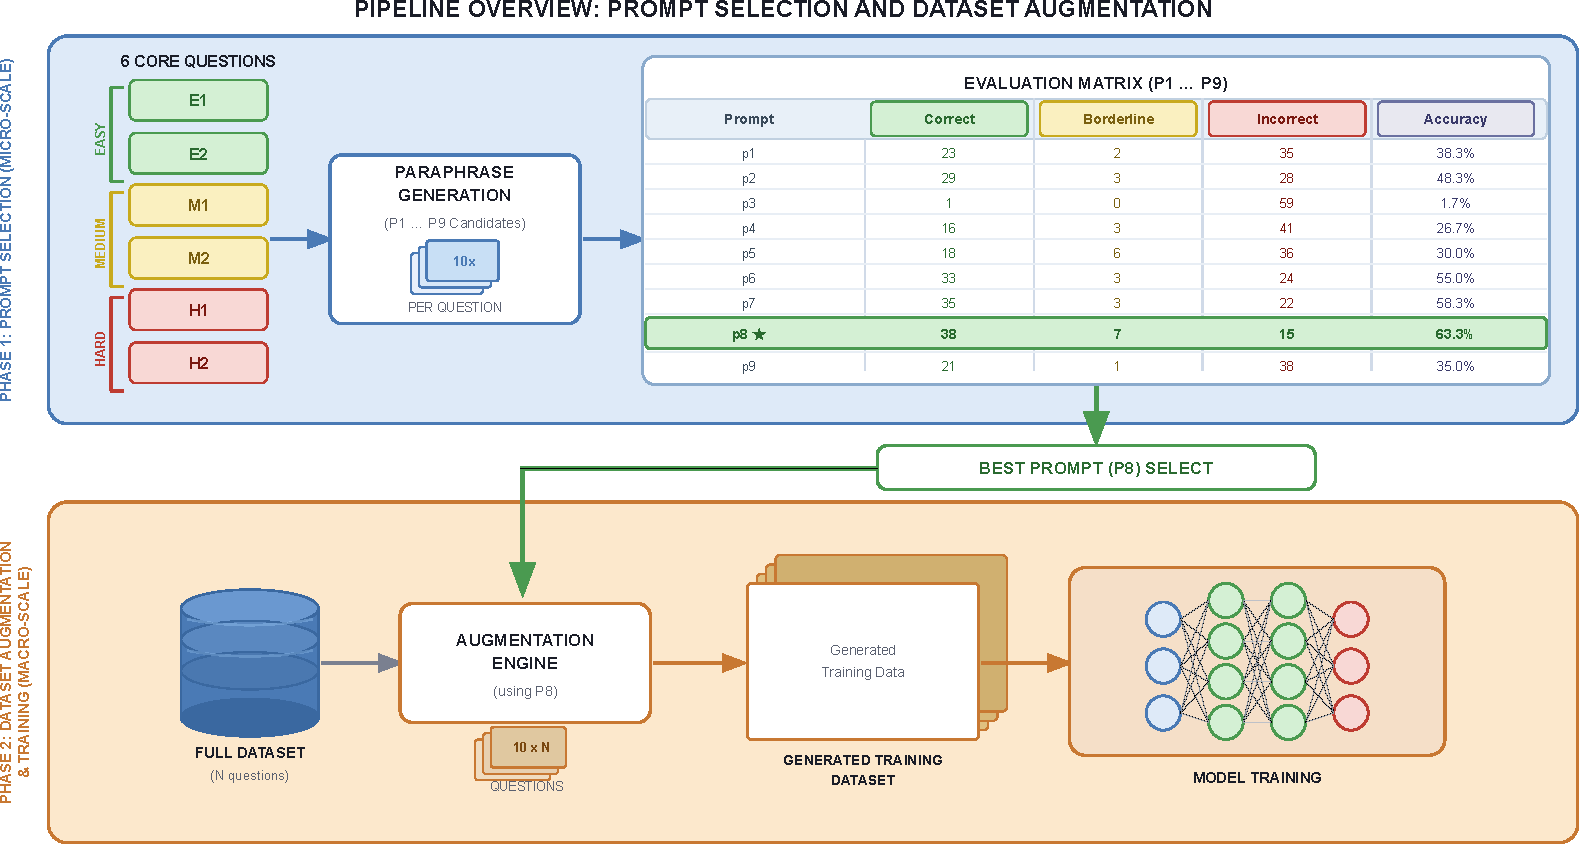
\includegraphics[width=\textwidth]{images/JURSE/pipeline.pdf}
  \caption{Overview of the LLM-based data augmentation pipeline.
  Unique questions from RSVQA-HR are grouped by difficulty and
  passed to LLaMA-2-7B with the selected prompt $p_8$. Ten
  reformulations are generated per question and added to the
  augmented dataset. The example panel illustrates the four
  possible evaluation outcomes for generated questions.}
  \label{fig:pipeline}
\end{figure}
 
It is important to note that no filtering step is
applied to the generated questions beyond the prompt
selection described above. While our manual evaluation
shows that a non-negligible proportion of generated
questions are borderline or incorrect (approximately
30--40\% depending on difficulty level), we chose to
include all generated questions in the augmented
dataset and rely on the model's ability to learn robust
representations despite the noise. This decision is
motivated by the scale of the augmentation: even at a
20\% error rate, the LLM-augmented training set
contains a far greater diversity of valid phrasings
than the original dataset. The impact of this noise
on model performance is analyzed in Section~\ref{sec:chap3_results}.

\begin{table}[ht]
\centering
\small
\caption{Examples of questions generated from the original
question \textit{``Are there more roads than parks?''}
using prompt $p_8$, along with their manual evaluation.}
\label{tab:generated_examples}
\begin{tabular}{ll}
\hline
\textbf{Evaluation} & \textbf{Generated Question} \\
\hline
Correct    & Is the number of roads greater than the number of parks? \\
Correct    & Do roads exceed parks in number? \\
Borderline & Can you name more roads than parks? \\
Incorrect  & Is the total distance of roads longer than the distance of parks? \\
\hline
\end{tabular}
\end{table}


 %============================================================
\section{Experimental Study}
\label{sec:chap3_experiments}
% ============================================================
 
\subsection{Dataset: RSVQA-HR}
\label{sec:chap3_dataset}
 
Our experiments are conducted on the RSVQA-HR
dataset~\cite{lobry2020rsvqa}, the high-resolution
benchmark of the RSVQA family. It uses orthoimagery
at 15\,cm resolution from the USGS data collection,
covering urban areas of the United States. The dataset
consists of 10,659 images and 955,664 question-answer
pairs distributed across four question types: presence
(\textit{e.g.}, \textit{``Is there a road?''}), area
(\textit{e.g.}, \textit{``What is the area covered by
grass?''}), count (\textit{e.g.}, \textit{``How many
buildings are there?''}), and comparison (\textit{e.g.},
\textit{``Are there more roads than parks?''}).
 
The dataset is divided into a training set
(625,340 question-answer pairs), a validation set
(102,843 pairs), test set 1 (222,684 pairs, covering
images similar in distribution to the training set),
and test set 2 (covering a city not seen during
training, used to evaluate geographic generalization).
This structure makes RSVQA-HR particularly well-suited
for evaluating generalization: test set 2 provides
a natural out-of-distribution evaluation that goes
beyond linguistic variation.
 
Following the augmentation procedure described in
Section~\ref{sec:chap3_pipeline}, the LLM-augmented
training set contains 6,878,740 question-answer pairs, 
more than ten times the original size. For
comparison, the back-translation-augmented training
set contains 1,739,794 pairs, as back translation
via three pivot languages (French, German, Chinese)
generates at most three additional versions per
question, with duplicates discarded.
 
\subsection{Experimental Setup}
\label{sec:chap3_setup}
 
\textbf{Model architecture.} Following the findings
of \cite{chappuis2023curse}, we use a dual-encoder
architecture as our RSVQA baseline. The visual branch
consists of a ResNet-152~\cite{he2016resnet} pretrained
on ImageNet and kept frozen during training. The
language branch consists of a
DistilBERT~\cite{sanh2019distilbert} encoder
fine-tuned during training. Visual and textual
representations are fused via point-wise
multiplication, followed by a multilayer perceptron
for answer prediction. This architecture is
representative of the encoder-based RSVQA paradigm
dominant at the time of this work and provides a
clean, reproducible baseline for evaluating the
effect of data augmentation independently of
architectural choices.
 
\textbf{Training conditions.} We train three separate
instances of this model on three different training
sets: the original unaugmented dataset (Original),
the LLM-augmented dataset (LLM-Aug), and the
back-translation-augmented dataset (BT-Aug). All
other hyperparameters are kept identical across
the three conditions to ensure that observed
differences in performance are attributable solely
to the training data.
 
\textbf{Evaluation protocol.} Each model is evaluated
on three test sets: the original test set 1
(Original), the LLM-augmented test set 1 (LLM-Aug),
and the back-translation-augmented test set 1
(BT-Aug). This cross-evaluation design (training
on one distribution, testing on another), allows
us to measure not only in-distribution performance
but also the degree to which each augmentation
strategy produces question distributions that are
genuinely novel and distinct from the original.
Overall accuracy and per-category accuracy are
reported.
 
\subsection{Results and Discussion}
\label{sec:chap3_results}
 
Table~\ref{tab:results} presents the cross-evaluation
results for all three models across all three test sets.
 
\begin{table*}[ht]
\centering
\footnotesize
\caption{Performance comparison of Original, LLM-Aug, and
BT-Aug models across different test sets. Accuracy (\%) per
question type. Avg = average across the three test sets.
Best per training condition in \textbf{bold}.}
\label{tab:results}
\begin{tabularx}{\textwidth}{
  l
  >{\centering\arraybackslash}X
  >{\centering\arraybackslash}X
  >{\centering\arraybackslash}X
  >{\centering\arraybackslash}X
  >{\centering\arraybackslash}X
  >{\centering\arraybackslash}X
  >{\centering\arraybackslash}X
  >{\centering\arraybackslash}X
  >{\centering\arraybackslash}X
  >{\centering\arraybackslash}X
  >{\centering\arraybackslash}X
  >{\centering\arraybackslash}X}
\toprule
& \multicolumn{4}{c}{\textbf{Train: Original}}
& \multicolumn{4}{c}{\textbf{Train: LLM-Aug}}
& \multicolumn{4}{c}{\textbf{Train: BT-Aug}} \\
\cmidrule(lr){2-5}\cmidrule(lr){6-9}\cmidrule(lr){10-13}
\textbf{Type}
& Orig & LLM & BT & Avg
& Orig & LLM & BT & Avg
& Orig & LLM & BT & Avg \\
\midrule
Presence
& 90.39 & 71.31 & 64.02 & 75.24
& \textbf{90.71} & \textbf{90.01} & 63.30 & \textbf{81.34}
& 69.82 & 65.05 & \textbf{68.58} & 67.82 \\
Area
& 81.45 & 23.75 & 64.45 & 56.55
& \textbf{83.88} & \textbf{83.45} & 59.13 & \textbf{75.49}
& 67.45 & 29.03 & \textbf{69.11} & 55.20 \\
Count
& 67.20 & 56.87 & 60.92 & 61.66
& \textbf{67.42} & \textbf{66.71} & \textbf{62.33} & \textbf{65.49}
& 64.57 & 52.02 & 63.57 & 60.39 \\
Comparison
& 89.66 & 56.71 & 70.00 & 72.12
& \textbf{89.91} & \textbf{86.90} & \textbf{67.65} & \textbf{81.49}
& 74.47 & 57.69 & 73.21 & 68.46 \\
\midrule
Overall
& 82.17 & 52.16 & 65.10 & 66.48
& \textbf{82.98} & \textbf{81.77} & 63.10 & \textbf{75.95}
& 69.07 & 50.95 & \textbf{68.37} & 62.80 \\
Average
& 82.78 & 55.70 & 65.13 & 67.87
& \textbf{83.35} & \textbf{81.93} & 63.72 & \textbf{76.33}
& 69.62 & 53.89 & \textbf{68.35} & 63.95 \\
\bottomrule
\end{tabularx}
\end{table*}
 
 
\textbf{In-distribution performance.}
The LLM-Aug model achieves an overall accuracy of
82.98\% on the original test set, slightly above the
Original model (82.17\%). This result is notable: despite
training on a dataset more than ten times larger and
with significantly more diverse phrasings, the LLM-Aug
model does not sacrifice in-distribution accuracy.
This suggests that the generated questions, while
more varied, do not introduce sufficient noise to
degrade performance on the original phrasing
distribution. The BT-Aug model also improves slightly
over the baseline on the original test set (69.07\%
overall), though the gap relative to the LLM-Aug
model is substantial.
 
\textbf{Generalization to augmented phrasings.}
When each model is tested on its own augmented test
set, a clear divergence emerges. The LLM-Aug model
achieves 81.77\% on the LLM-augmented test set,
close to its in-distribution performance, indicating
that the representations it learned are genuinely
robust to paraphrase variation. By contrast, the
Original model drops to 52.16\% on the LLM-augmented
test set, a degradation of nearly 30 percentage
points. This drop confirms two things: first,
that the LLM-generated questions are genuinely
distinct from the originals in terms of surface form;
second, that the Original model has overfit to the
specific phrasings present in the training data and
fails to generalize.
 
\textbf{Question type analysis.}
The area category shows the largest performance gap.
The Original model drops from 81.45\% on the original
test set to 23.75\% on the LLM-augmented test set.
This is consistent with the difficulty grouping
analysis in Section~\ref{sec:chap3_difficulty}: area
questions tend to involve complex spatial descriptions
that are hardest to paraphrase faithfully, meaning
the LLM-generated area questions are the most
linguistically distant from their originals. The
count and comparison categories are more robust,
likely because the core quantitative structure of
these questions is preserved even under paraphrasing.
 
\textbf{Back translation results.}
Both models show a performance drop on the
BT-augmented test set, with the Original model
retaining a slight advantage (approximately 2\%
on overall accuracy). This can be attributed to
two properties of back translation: first, BT-generated
questions tend to remain structurally close to the
originals, so the Original model partially recognizes
them; second, some BT outputs are of lower quality
due to translation errors, which both penalizes the
BT-Aug model during training and introduces harder
test examples. The BT-Aug model performs notably
lower on its own test set than the LLM-Aug model
does on the LLM-augmented test set (68.37\% vs.
81.77\%), suggesting that BT augmentation introduces
more noise and less useful diversity than LLM-based
augmentation.
 
\textbf{Cross-augmentation generalization.}
An interesting pattern emerges when models are
evaluated on a test set produced by a different
augmentation strategy than the one used for training.
All models degrade significantly in this setting,
which confirms that the two augmentation methods
produce genuinely different linguistic distributions.
This result also highlights a limitation of our
evaluation framework: robustness to one type of
paraphrase does not automatically transfer to
robustness to another. Future work could explore
hybrid training strategies that combine multiple
augmentation sources to produce more universally
robust representations.
 
% ============================================================
\section{Conclusion and Limitations}
\label{sec:chap3_conclusion}
% ============================================================
 
In this chapter, we addressed the generalization problem
in RSVQA from a data-centric perspective. We proposed
a question augmentation framework leveraging LLaMA-2-7B
to generate ten semantically equivalent reformulations
of each question in the RSVQA-HR dataset, guided by a
prompt selected through systematic evaluation of nine
candidates across questions of varying linguistic
complexity. Experimental results demonstrate that models
trained on LLM-augmented data achieve higher robustness
to unseen phrasings than models trained on the original
dataset or on back-translation-augmented data, while
maintaining competitive in-distribution accuracy. The
cross-evaluation design further confirms that LLM-generated
questions constitute a genuinely novel and challenging
distribution, distinct from both the original and
back-translated phrasings.
 
\textbf{Limitations.}
Several limitations of this work should be acknowledged.
First, experiments are conducted exclusively on RSVQA-HR,
which covers urban areas of the United States. Whether
the proposed augmentation strategy generalizes to rural
datasets~\cite{lobry2021rsvqaben}, to datasets involving
SAR imagery~\cite{tosato2024sar}, or to geographically
diverse regions remains an open question.
Second, only a single LLM (LLaMA-2-7B) is evaluated.
Larger models in the LLaMA-2 family (13B, 70B) or
other instruction-tuned models may produce higher-quality
paraphrases, particularly for hard questions involving
complex spatial relations. A systematic comparison of
LLM quality and scale on augmentation performance is
left for future work.
Third, the prompt evaluation is conducted on a small
manually reviewed subset. While the selected prompt
($p_8$) achieves the highest accuracy in this evaluation,
the review process does not measure inter-annotator
agreement, and the borderline category introduces
subjectivity into the quality assessment.
Finally, it remains to be verified whether the benefits
of LLM-based augmentation transfer to more recent
generative RSVQA architectures based on large
vision-language models, where the base model already
possesses significant linguistic diversity from
pre-training.
 
\textbf{Perspectives.}
Future work could explore hybrid augmentation strategies
combining LLM-based question generation with image-level
augmentation or answer-aware generation. The compatibility
of the proposed approach with semantic-based RSVQA
methods~\cite{tosato2024segguided} also warrants
investigation. More broadly, this work highlights the
importance of data diversity as a first-class concern
in RSVQA research, complementary to architectural
innovations.
 
While this chapter addressed generalization from
a data perspective, the following chapter investigates
how model architecture itself can be improved to better
exploit the spatial structure present in remote sensing
imagery. Specifically, how segmentation maps can be
used to guide visual attention in RSVQA models.
 
% ============================================================
%  CHAPTER 4 — Segmentation-Guided Attention for RSVQA
% ============================================================
% To include in main.tex use:  \input{chapter4}
% Paper source: IGARSS 2024 — Tosato*, Boussaid* et al.
%
% Required packages in main.tex preamble:
%   \usepackage{booktabs}
%   \usepackage{tabularx}
%   \usepackage{multirow}
%   \usepackage{array}
% ============================================================

\chapter{Segmentation-Guided Attention for Remote Sensing Visual Question Answering}
\label{chap:seg_attention}
\startcontents[chapters]

\printmyminitoc{
	%\lipsum[1]
\textit{Chapter summary.} Standard RSVQA attention mechanisms compute attention weights directly from raw visual features, forcing the model to jointly discover relevant semantic categories and their spatial extent from supervision alone. This chapter instead guides attention with an explicit, multi-channel segmentation prior: a frozen UPerNet/Swin Transformer module, trained on 16 BD TOPO object classes, produces per-class spatial maps that condition attention jointly with the question. Evaluated on a preliminary TAMMI dataset over four Île-de-France departments, the proposed model improves overall accuracy by approximately 10\% over a no-attention baseline and 5\% over vanilla attention.
}
% ============================================================
\section{Introduction}
\label{sec:chap4_intro}
% ============================================================

The previous chapter addressed the generalization problem
in RSVQA from a data perspective, showing that LLM-based
question augmentation can improve model robustness to
unseen phrasings. However, data diversity alone does not
address a more fundamental limitation: the capacity of the
model to correctly identify and locate the visual content
relevant to a given question. In dense remote sensing scenes,
where multiple object classes coexist at varying scales and
spatial configurations, standard visual encoders tend to
produce globally averaged representations that fail to capture
the fine-grained spatial structure required for accurate
question answering. This chapter addresses this limitation
from an architectural perspective, proposing a method that
explicitly guides the model's visual attention using semantic
segmentation.

Attention mechanisms have become a cornerstone of visual
question answering pipelines. By weighting different spatial
regions of the visual feature map according to their relevance
to the input question, attention allows the model to
selectively focus on the parts of the image most informative
for answering. This has been shown to consistently improve
performance in general VQA~\cite{zhang2020context,
wei2020multimodality}, and has been adapted to the RSVQA
setting by~\cite{zheng2021mutual}, who propose a mutual
attention inception network that aligns spatial positions
with question words. However, existing attention mechanisms
in RSVQA operate directly on raw visual features, without
any explicit semantic understanding of the scene content.
In the context of remote sensing, where the visual appearance
of object classes (roads, buildings, vegetation, water areas)
is highly variable across regions, this lack
of semantic grounding limits the precision with which
attention can localize the relevant content.

Semantic segmentation provides exactly the kind of
structured, class-level understanding of the scene that
raw visual features lack. By explicitly identifying which
pixels belong to which object class, a segmentation map
encodes a rich spatial layout of the image that is directly
aligned with the semantic content of RSVQA questions,
which almost always refer to specific object classes
(\textit{e.g.}, \textit{``Is there a road?''}, \textit{``What
is the area of the water zone?''}). In the natural image
domain, segmentation has been used to guide attention in
VQA~\cite{gan2017vqs} and to produce faithful visual
explanations~\cite{wu2018faithful}. To the best of our
knowledge, however, this approach had not been explored in
the remote sensing VQA literature at the time of this work.

In this chapter, we propose to embed a segmentation-guided
attention mechanism into a RSVQA pipeline. A key original
aspect of this design is the use of \textit{multi-channel}
segmentation maps, one binary channel per object class,
rather than the traditional single-channel segmentation in
which each pixel receives a single class label. This choice
is motivated by the frequent spatial overlap between object
classes in remote sensing imagery (\textit{e.g.}, a road
passing through a vegetation zone), which a single-channel
representation cannot capture but which a multi-channel one
represents naturally, as detailed in
Section~\ref{sec:chap4_seg_multichannel}. The segmentation
itself is performed by a UPerNet model with a Swin
Transformer backbone~\cite{liu2021swin}, trained on 16
object classes derived from the BD TOPO geographic
database~\cite{bdtopo} and then kept frozen during VQA
training. The resulting 16-channel segmentation maps are
used to guide the computation of attention weights jointly
with the question representation, providing the model with
an explicit semantic prior over the spatial
layout of the scene that raw visual features alone do not
supply. We evaluate this approach on a new
dataset built from very high resolution airborne imagery
(BD ORTHO~\cite{bdortho}) over four
departments of the Île-de-France region, which constitutes
a preliminary version of the TAMMI dataset introduced in
full in Chapter~\ref{chap:tammi}. Our ablation study
demonstrates gains of approximately 10\% in overall
accuracy over a baseline without attention, and 5\% over
a vanilla attention mechanism without segmentation guidance.

The remainder of this chapter is organized as follows.
Section~\ref{sec:chap4_rw} reviews related work on
attention mechanisms and segmentation-guided approaches
in VQA. Section~\ref{sec:chap4_dataset} describes the
dataset and segmentation annotations used in this work.
Section~\ref{sec:chap4_method} presents the proposed
architecture. Section~\ref{sec:chap4_experiments} details
the experimental results and ablation study.
Section~\ref{sec:chap4_conclusion} concludes with
limitations and perspectives.

% ============================================================
\section{Related Work}
\label{sec:chap4_rw}
% ============================================================
% Scope: specific to this contribution only.
% General VQA task definition, RS background, and broad
% vision-language architectures are in Ch. 2.
% Ch. 3 already covered data augmentation and linguistic bias.
% Here: attention in VQA, segmentation-guided vision, RSVQA attention.
This section reviews the two bodies of work this chapter connects. 
Section~\ref{sec:chap4_rw_attention} reviews attention mechanisms 
in VQA generally and in RSVQA specifically, where attention is computed 
directly from raw visual features. Section~\ref{sec:chap4_rw_seg} then reviews work that instead guides attention with an explicit 
semantic segmentation prior, established in the natural image domain but, at the time of this work, unexplored in RSVQA.
\subsection{Attention Mechanisms in Visual Question Answering}
\label{sec:chap4_rw_attention}

Attention mechanisms were introduced in VQA to address a
key limitation of early models, which represented an
entire image with a single global feature vector,
regardless of the question being asked.
\textcite{yang2016stacked} propose Stacked Attention
Networks (SAN), which use the semantic representation of
the question as a query to iteratively search for
relevant image regions, performing multiple steps of
attention to progressively refine the focus of the model.
\textcite{anderson2018bottomup} further refine this idea with
a bottom-up and top-down attention mechanism, in which a
bottom-up module (based on Faster R-CNN) proposes
object-level image regions, while a top-down mechanism
determines which of these regions are relevant to the
question. This object-centric formulation of attention
became a standard component of VQA architectures, as it
aligns naturally with the object-oriented phrasing of most
questions.

In the RSVQA setting, \textcite{zheng2021mutual} propose a
mutual attention inception network that computes attention
weights by modeling the alignment between spatial image
positions and question words, using an inception-based
visual backbone. This work demonstrates that attention
improves performance on RSVQA benchmarks, in a manner
consistent with findings in the natural image domain.
However, in the approaches discussed above,
including those applied to remote sensing, attention
weights are computed directly from raw visual features,
without any explicit intermediate representation of the
scene's semantic content. The attention mechanism must
therefore implicitly learn both \textit{what} the relevant
semantic categories are and \textit{where} they are
located, from the VQA supervision signal alone. This
joint demand is particularly challenging in remote
sensing imagery, where object classes are visually
ambiguous at a given resolution and the training signal
for any single question type is comparatively sparse.

\subsection{Segmentation as a Prior for Visual Reasoning}
\label{sec:chap4_rw_seg}

An alternative line of work proposes to decouple these two
demands by providing the attention mechanism with an
explicit semantic segmentation of the scene, computed as
a separate task. \textcite{gan2017vqs} introduce the VQS
dataset, which links segmentation annotations to
question-answer pairs, and show that supervising attention
with segmentation masks improves both VQA accuracy and
the interpretability of the resulting attention maps, while
also enabling question-focused semantic segmentation as a
complementary output. \textcite{wu2018faithful} pursue a
related goal from the perspective of explainability,
proposing a multimodal explanation framework in which
segmentation-derived attention maps are used to generate
visual justifications for predicted answers that are
faithful to the model's actual reasoning process, as
opposed to post-hoc visualizations that may not reflect
the features actually used for prediction.

Both lines of work demonstrate, in the natural image
domain, that segmentation provides a more informative and
more interpretable prior for attention than raw visual
features alone: it supplies the attention mechanism with
an explicit, class-level representation of the scene,
removing the need to jointly discover semantic categories
and their spatial extent from VQA supervision alone. To
the best of our knowledge, at the time of this work, this
strategy had not been explored in the remote sensing VQA
literature, despite the fact that remote sensing benefits
from a particularly rich source of segmentation-relevant
annotations through geographic databases such as BD
TOPO~\cite{bdtopo}. This chapter addresses this gap by
introducing a segmentation-guided attention mechanism for
RSVQA, using multi-channel segmentation maps derived from
such a geographic database as an explicit semantic prior.

% ============================================================
\section{Dataset and Segmentation Annotations}
\label{sec:chap4_dataset}
% ============================================================

\subsection{Very High Resolution Imagery}
\label{sec:chap4_dataset_vhr}

The experiments in this chapter are conducted on a
preliminary version of the TAMMI dataset, introduced in
full in Chapter~\ref{chap:tammi}. We provide here a concise
overview of the data used.

The visual inputs consist of very high resolution (VHR)
airborne RGB orthophotos from the BD ORTHO
database~\cite{bdortho}, produced by the French National
Geographic Institute (IGN) at a ground resolution of 20\,cm.
The images are subdivided into patches of
$1000 \times 1000$ pixels, each covering an area of
$200\,\text{m} \times 200\,\text{m}$ on the ground. We
select four adjacent departments from the Île-de-France
region (Paris, Hauts-de-Seine, Val-de-Marne, and
Seine-Saint-Denis) resulting in 16,274 patches. The
dataset is split into training (60\%), validation (20\%),
and test (20\%) sets, with the same split applied to both
the segmentation task and the VQA task.

\subsection{Segmentation Annotations from BD TOPO}
\label{sec:chap4_dataset_seg}

A key characteristic of this dataset, and the aspect most
directly relevant to the contribution of this chapter, is
the availability of dense segmentation annotations derived
from the BD TOPO database~\cite{bdtopo}, a vectorial
description of the French territory maintained by IGN.

\subsubsection{Class taxonomy}
\label{sec:chap4_seg_classes}

We define 16 segmentation classes organized into six
thematic groups, reflecting the semantic categories most
relevant to RSVQA questions over urban and peri-urban
areas:

\begin{itemize}
    \item \textbf{Buildings:} Building, Cemetery, Sports
    Field, Water Tank, Pylon, Surface Construction;
    \item \textbf{Land Use:} Foreshore Zone, Vegetation
    Zone;
    \item \textbf{Water Area;}
    \item \textbf{Transport:} Airfield, Transportation
    Construction, Road, Railway;
    \item \textbf{Regulated Areas:} Public Forest,
    National Park;
    \item \textbf{Services and Activities:} Museums,
    Monuments, Schools, and similar entities.
\end{itemize}

The choice of 16 classes reflects a trade-off between
semantic richness and annotation density: finer-grained
taxonomies would yield sparser annotations in urban areas,
while coarser ones would lose the class-level specificity
required to guide attention toward the objects referenced
in RSVQA questions.

\subsubsection{Multi-channel segmentation}
\label{sec:chap4_seg_multichannel}

A critical design choice in this work is the use of
\textit{multi-channel} segmentation maps rather than the
traditional single-channel representation. In standard
semantic segmentation, each pixel is assigned a single
class label, which implicitly assumes that object classes
do not overlap spatially. This assumption is frequently
violated in remote sensing imagery, where objects from
different classes can occupy the same pixel footprint at
the given resolution (\textit{e.g.}, a road passing through
a vegetation zone, or a building adjacent to a water area).

Our multi-channel representation instead produces one
binary channel per class, where each channel independently
indicates the presence or absence of that class at each
spatial location. This allows overlapping object classes
to be represented simultaneously, providing a richer and
more faithful description of the scene layout. Concretely,
the segmentation output $f_\text{seg} \in \mathbb{R}^{16
\times H \times W}$, with $H = W = 1000$ matching the
$1000 \times 1000$ pixel resolution of the input VHR patch
$p_\text{VHR}$ (Section~\ref{sec:chap4_dataset_vhr}), encodes the full spatial distribution
of all 16 classes over the image, which is then used
directly to guide the attention computation.

\subsubsection{Segmentation module training}
\label{sec:chap4_seg_training}

The segmentation module consists of a UPerNet
architecture~\cite{xiao2018upernet} with a Swin
Transformer backbone~\cite{liu2021swin}, pre-trained on
the ADE20K dataset~\cite{zhou2019ade20k}, a large-scale
semantic segmentation benchmark of roughly 25,000 natural
images annotated with 150 object and stuff categories
spanning indoor and outdoor scenes. While ADE20K's imagery
and class taxonomy differ substantially from remote sensing,
pre-training on it still provides the backbone with
general-purpose visual features, rather than
starting from randomly initialized weights. A convolutional
layer is added to map the feature maps $f_\text{seg}$ to
the 16-channel output, which is then bilinearly interpolated
to the spatial resolution of the input patch $p_\text{VHR}$.

We fine-tune this segmentation module on the 16-class
annotations described above, using the same training split
as the VQA task. After training, the weights of the
segmentation module are \textbf{frozen} before the VQA
pipeline is trained. This design choice is motivated by two
considerations. First, freezing the segmentation module
ensures that the attention mechanism learns to exploit the
semantic layout produced by segmentation rather than
co-adapting with it, which would risk collapsing the
segmentation representations toward features that are
useful for VQA but not necessarily semantically meaningful.
Second, it decouples the two training objectives, making
the overall pipeline more stable and interpretable.

\subsection{Question/Answer Pairs}
\label{sec:chap4_dataset_qa}

The dataset contains 146,848 question/answer pairs
distributed across nine question types organized into
four categories, summarized in Table~\ref{tab:chap4_qtypes}.
Questions are generated automatically from the BD TOPO
annotations following a two-stage procedure designed to
balance both question type and answer type distributions,
reducing language biases~\cite{chappuis2025langbias}. Question
type is balanced first, by randomly generating ten questions
per question type for each VHR patch $p_\text{VHR}$. Answer
type is then balanced by defining, for each question type, a
maximum number of questions per answer type, $N_{Q,A}$; only
questions whose answer type is less represented than
$N_{Q,A}$ are retained. To reach a sufficient number of
questions under this filtering, the VHR patches are browsed
twice. The full
question generation methodology is described in
Chapter~\ref{chap:tammi}.

\begin{table}[ht]
\centering
\small
\caption{Question type taxonomy used in the dataset.
Nine question types are organized into four categories.
Abbreviations used in Table~\ref{tab:chap4_results}
are shown in parentheses.}
\label{tab:chap4_qtypes}
\begin{tabularx}{\textwidth}{l >{\raggedright\arraybackslash}X}
\toprule
\textbf{Category} & \textbf{Question types} \\
\midrule
Class questions & Presence, Count, Density \\
Object questions & Absolute location, Area \\
Two-class questions & Comparison \\
Object relation questions & Relative location, Distance,
                            Nearest object \\
\bottomrule
\end{tabularx}
\end{table}

The distribution of answers across question types is
illustrated in Figure~\ref{fig:chap4_dist}. Each sector
of the chart corresponds to one question type, and the
inner ring shows the distribution of answers within that
type. For numerical answers (count, area, distance), only
the ordering is shown without explicit labeling, with
maximum values of 280 (count), 40,000\,m$^2$ (area), and
273\,m (distance). The chart confirms that the balancing
procedure successfully avoids extreme answer skew within
each question type, which is critical for training models
that are robust to linguistic bias.

\begin{figure}[ht]
    \centering
    % NOTE: insert Figure 1 from the paper here
    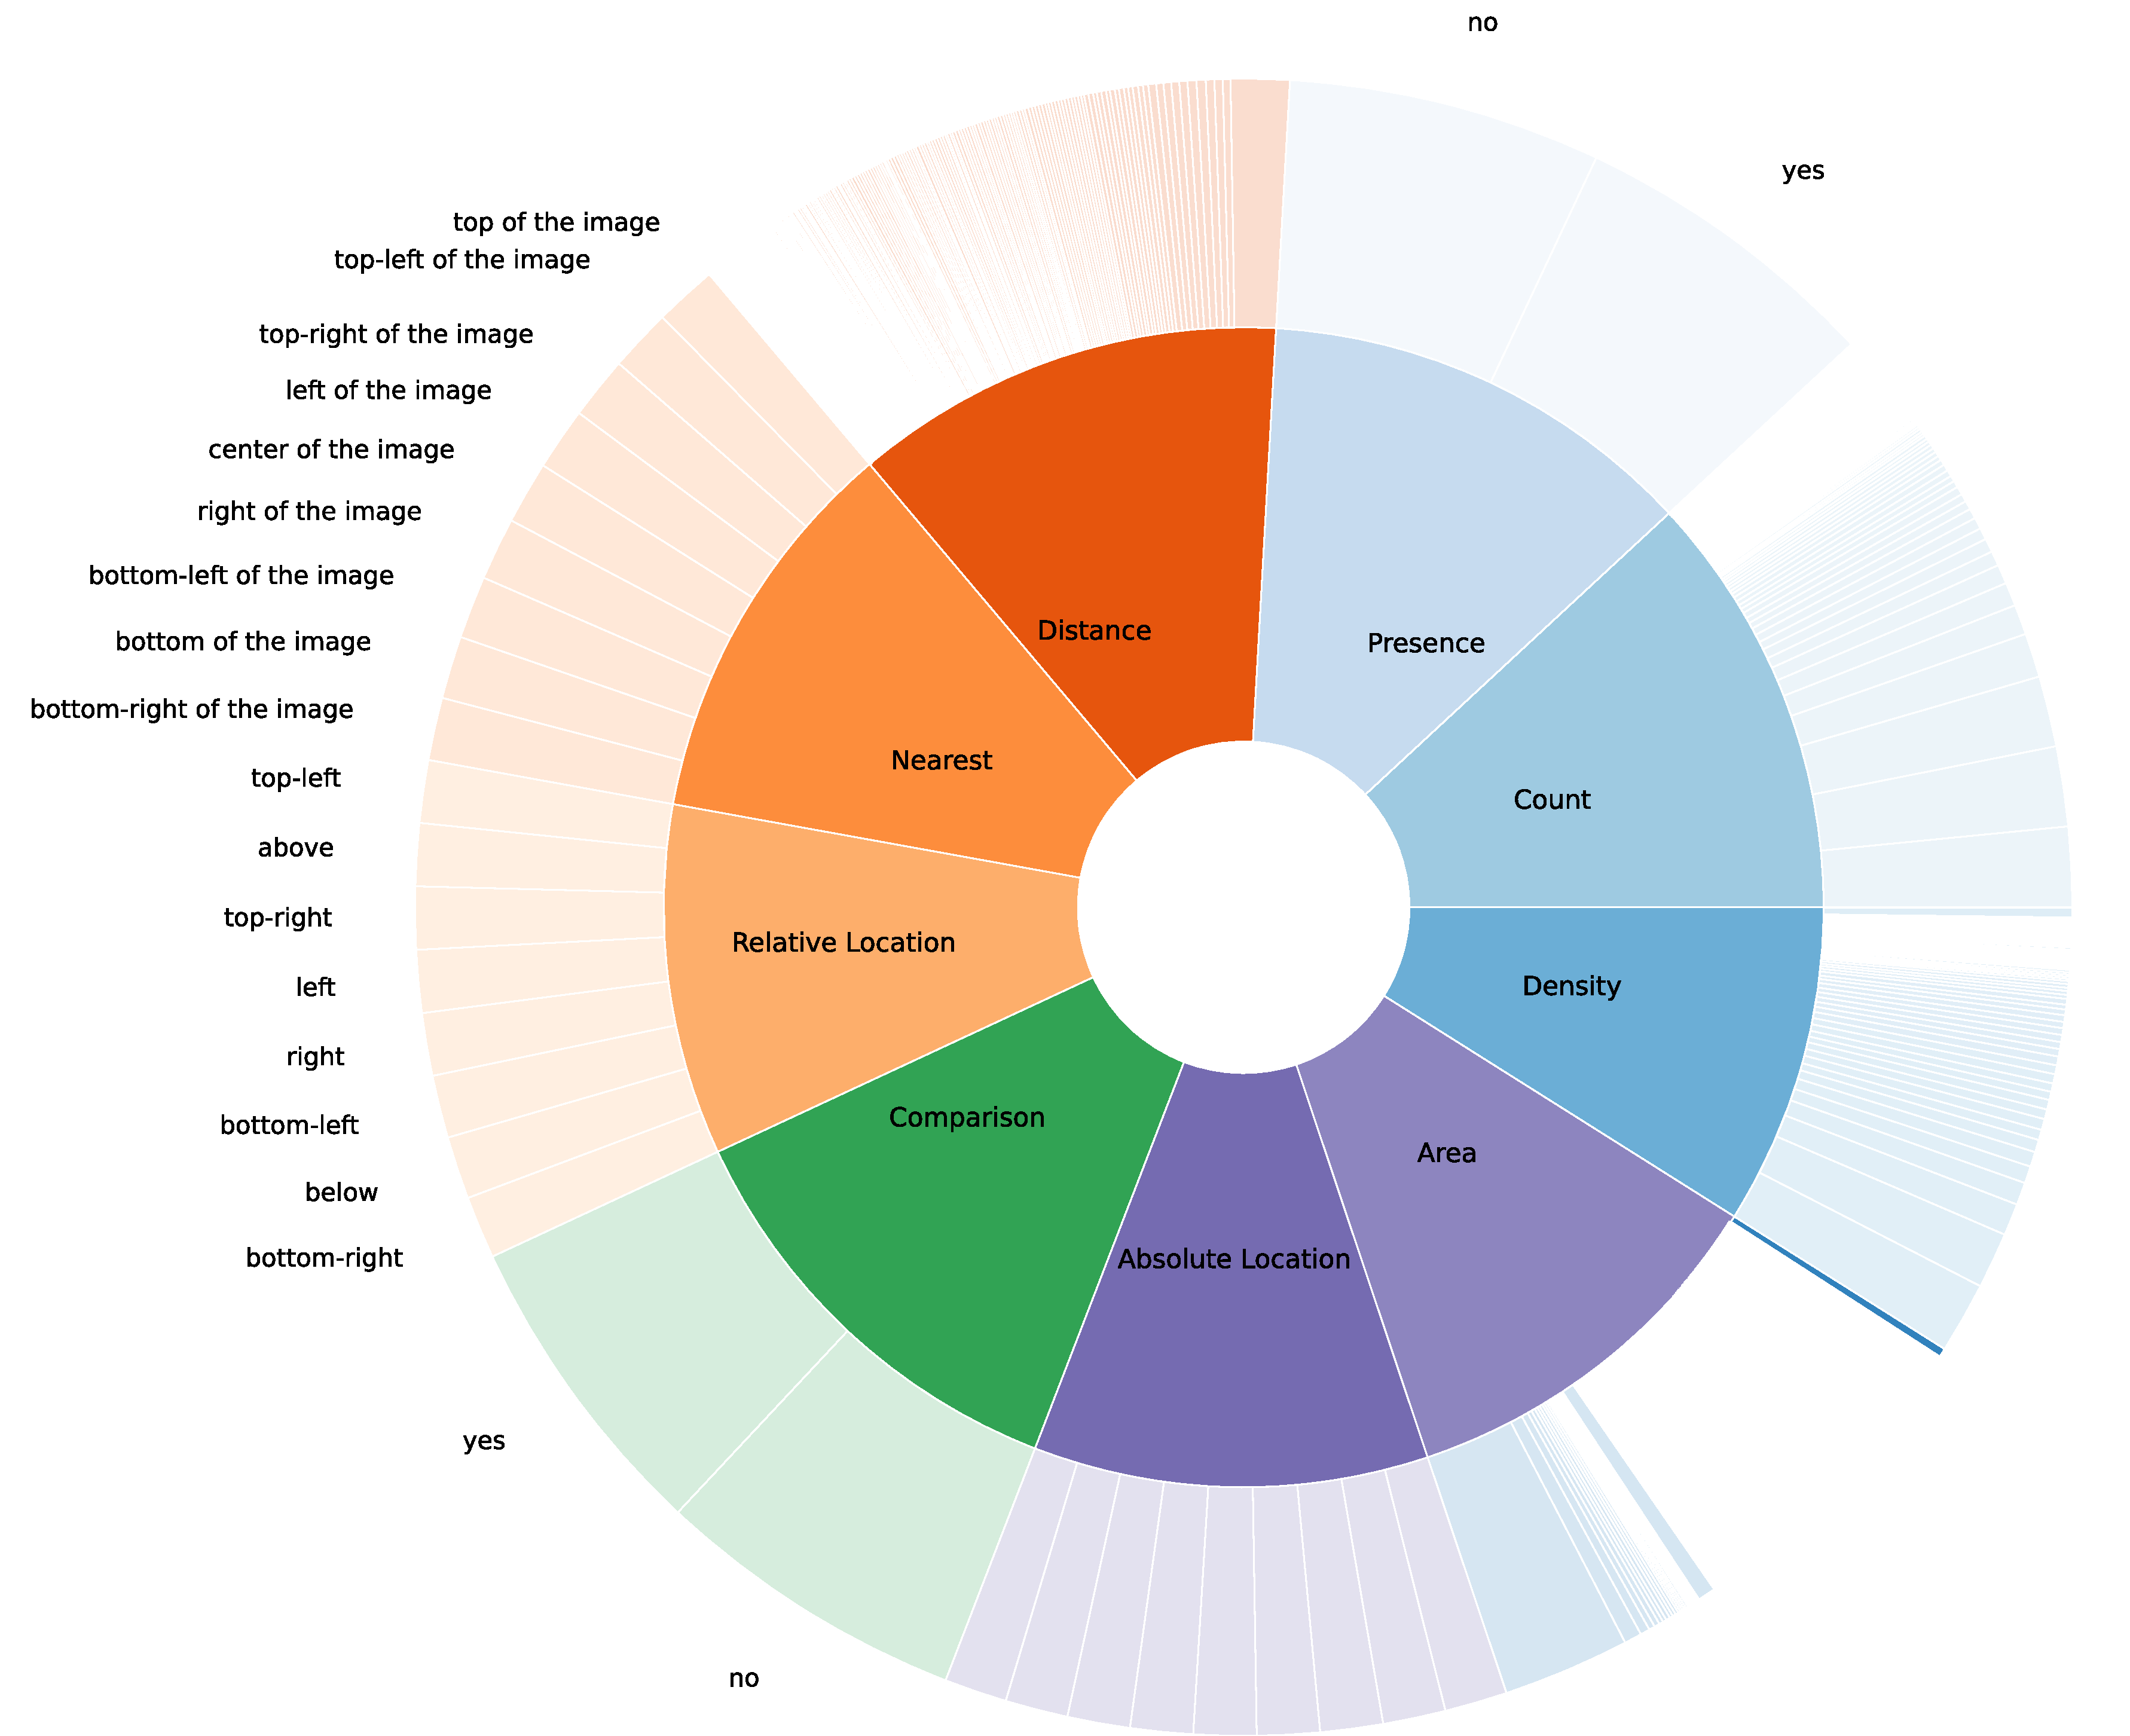
\includegraphics[width=0.7\textwidth]{images/Seg/newtry.pdf}
    \caption{Distribution of answers by question type.
    Numerical answer labels are omitted and shown in
    order only. Maximum values: 280 (count), 40,000\,m$^2$
    (area), 273\,m (distance). The balanced distribution
    across answer types within each question category
    reduces language bias during training.}
    \label{fig:chap4_dist}
\end{figure}

% ============================================================
\section{Segmentation-Guided Attention Architecture}
\label{sec:chap4_method}
% ============================================================
This section presents the proposed architecture in four parts: Section~\ref{sec:chap4_method_overview} gives a high-level overview of the full pipeline, Section~\ref{sec:chap4_method_features} details the frozen visual and textual feature extractors, Section~\ref{sec:chap4_method_attention} presents the segmentation-guided attention module itself, and Section~\ref{sec:chap4_method_prediction} describes the prediction head and training procedure.
\subsection{Overview}
\label{sec:chap4_method_overview}

We introduce a RSVQA pipeline that incorporates
segmentation as an explicit prior for the attention
mechanism. The pipeline takes as input a VHR patch
$p_\text{VHR}$ and a natural language question $q$, and
produces a predicted answer from a closed vocabulary of
1,000 classes. It consists of three components: a feature
extraction module, a segmentation-guided attention module,
and a prediction head. Figure~\ref{fig:chap4_arch}
illustrates the full architecture.

 \begin{figure}[ht]
   \centering
   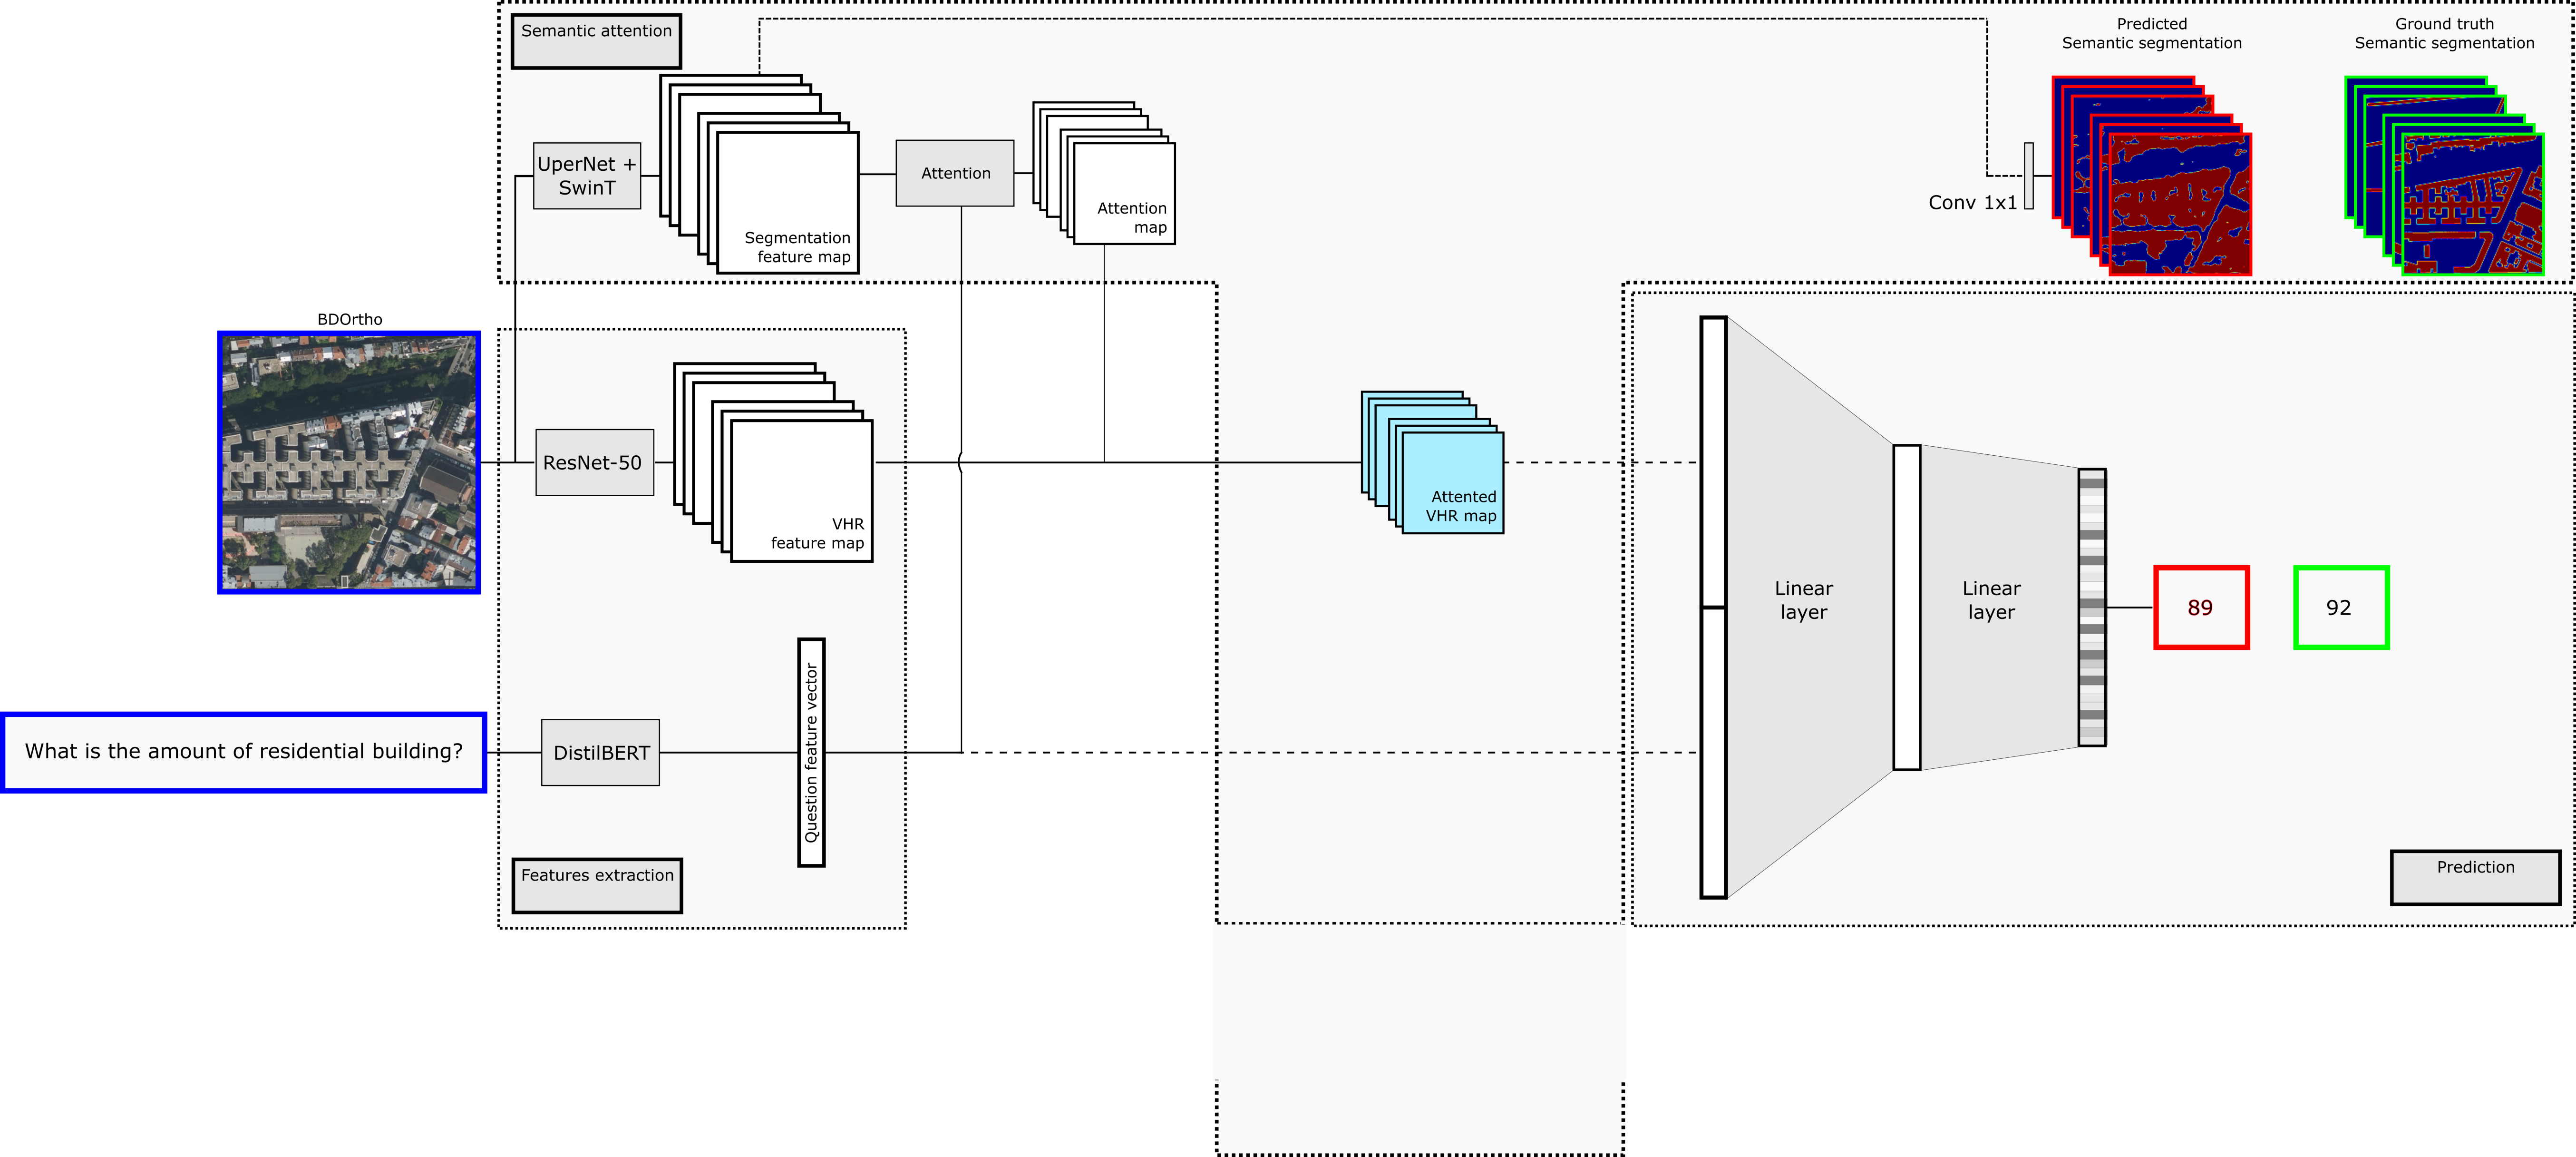
\includegraphics[width=\textwidth]{images/Seg/model1_1.png}
   \caption{Architecture of the proposed segmentation-guided
   attention pipeline. Inputs (VHR image and question) are
   shown in blue; outputs (answer prediction and segmentation)
   in red; ground truths in green.}
   \label{fig:chap4_arch}
 \end{figure}

\subsection{Feature Extraction}
\label{sec:chap4_method_features}

\textbf{Visual features.} Visual features $f_\text{VHR}$
are extracted from the VHR patch using a ResNet-50
model~\cite{he2016resnet} pre-trained on ImageNet, from
which the final fully-connected layer is removed. The
ResNet-50 weights are kept frozen throughout training.
The choice of ResNet-50 over larger variants is
deliberate: rather than relying on a more powerful visual
backbone to compensate for the lack of semantic grounding,
this work shows that even with a comparatively modest
encoder, explicitly guiding attention with segmentation
yields improvements. ResNet-50 remains a
strong and widely-used baseline in its own right.

\textbf{Textual features.} Textual features $f_q$ are
extracted from the question $q$ using a DistilBERT
encoder~\cite{sanh2019distilbert}, also kept frozen. The
use of frozen encoders for both modalities ensures that
the training signal is directed toward the attention and
fusion modules rather than toward refining the base
representations, which stabilizes the learning process
given the relatively modest size of the dataset.

\subsection{Segmentation-Guided Attention}
\label{sec:chap4_method_attention}

The segmentation-guided attention module computes a
spatial attention map $\mathbf{a}$ that is applied to the
visual features $f_\text{VHR}$, emphasizing regions
relevant to the question. The computation proceeds as
follows.

The textual features $f_q$ are projected to a
250-dimensional space via a linear layer with dropout
$d = 0.5$:

\begin{equation}
    \tilde{f}_q = \text{Dropout}(W_q f_q + b_q),
    \quad \tilde{f}_q \in \mathbb{R}^{250}
\end{equation}

Simultaneously, the segmentation feature map
$f_\text{seg} \in \mathbb{R}^{16 \times H \times W}$ is
projected to a 250-channel spatial representation via a
$1 \times 1$ convolution with dropout $d$:

\begin{equation}
    \tilde{f}_\text{seg} = \text{Dropout}(\text{Conv}_{1
    \times 1}(f_\text{seg})),
    \quad \tilde{f}_\text{seg} \in \mathbb{R}^{250 \times
    H \times W}
\end{equation}

The two representations are concatenated along the channel
dimension (broadcasting $\tilde{f}_q$ spatially), and a
ReLU activation followed by a $1 \times 1$ convolution
produces a single-channel attention glimpse:

\begin{equation}
    \mathbf{a} = \text{Conv}_{1 \times 1}\left(
    \text{ReLU}\left([\tilde{f}_q \oplus
    \tilde{f}_\text{seg}]\right)\right),
    \quad \mathbf{a} \in \mathbb{R}^{1 \times H \times W}
\end{equation}

The attention map $\mathbf{a}$ is then applied element-wise
to the visual features:

\begin{equation}
    \hat{f}_\text{VHR} = \mathbf{a} \odot f_\text{VHR}
\end{equation}

The key insight of this design is that the attention weights
are conditioned on \textit{both} the question semantics
(via $\tilde{f}_q$) and the spatial class layout (via
$\tilde{f}_\text{seg}$). This allows the model to focus
on image regions that are simultaneously relevant to the
question and semantically coherent, for instance,
attending to road pixels when answering a question about
roads, rather than activating on arbitrary high-contrast
regions.

\subsection{Prediction Head and Training}
\label{sec:chap4_method_prediction}

The attended visual features $\hat{f}_\text{VHR}$ are
concatenated with the textual features $f_q$ to form a
global multimodal representation. This is passed through
a 2-layer MLP with ReLU activations and dropout $d$,
producing a 1,000-dimensional output corresponding to the
1,000 most frequent answers in the training set.

The model is trained end-to-end (excluding the frozen
encoders and segmentation module) using a cross-entropy
loss, optimized with Adam at a learning rate of $10^{-6}$
and a batch size of 4. Training runs for approximately
100 hours on a single NVIDIA V100-16G GPU.

% ============================================================
\section{Experimental Study}
\label{sec:chap4_experiments}
% ============================================================
This section evaluates the proposed architecture in two stages. 
Section~\ref{sec:chap4_seg_results} first evaluates the segmentation module on its own,
 since the quality of the semantic prior it provides directly bounds what segmentation-guided attention can achieve downstream. 
 Section~\ref{sec:chap4_vqa_results} then evaluates the full VQA pipeline against two ablations, 
isolating the respective contributions of attention and of segmentation guidance specifically.
\subsection{Segmentation Results}
\label{sec:chap4_seg_results}

The segmentation module is evaluated independently on the
validation set using a precision-recall curve with 20
thresholds, identifying the optimal per-class threshold.
The model achieves an overall precision of 53.6\%, an
overall recall of 73.2\%, and an overall F1-score of
60.1\% on the test set. The relatively higher recall than precision
reflects the characteristics of the multi-channel
formulation: since each channel independently detects
one class, the model tends toward inclusive detection
(fewer missed objects) at the cost of some false
positives. These results confirm that the segmentation
module produces meaningful spatial class maps, providing
a reliable semantic prior for the attention mechanism.

While an F1-score of 60.1\% would be modest as a
standalone segmentation benchmark for 16-class land cover
classification, the goal of this module is not to achieve
state-of-the-art segmentation but to provide a sufficiently
informative semantic prior for the attention mechanism.
As shown in Section~\ref{sec:chap4_vqa_results}, even at
this level of quality, the segmentation maps yield a
measurable improvement in VQA accuracy, indicating that
the attention mechanism is able to extract useful spatial
and semantic structure from imperfect segmentation
predictions.

\subsection{VQA Results and Ablation Study}
\label{sec:chap4_vqa_results}

Table~\ref{tab:chap4_results} presents the per-question
type accuracy, overall accuracy (OA), and average accuracy
(AA) for the proposed model and two ablation variants:

\begin{itemize}
    \item \textbf{Proposed}: full model with
    segmentation-guided attention;
    \item \textbf{A1}: vanilla attention without
    segmentation guidance;
    \item \textbf{A2}: no attention mechanism.
\end{itemize}

\begin{table}[ht]
\centering
\small
\begin{tabular}{l ccc}
\toprule
\multirow{2}{*}{\textbf{Question type}}
  & \textbf{Proposed} & \textbf{A1} & \textbf{A2} \\
  & (Attention + Segmentation) & (Attention only) & (No attention) \\
\midrule
Presence & \textbf{89.36} & 85.79 & 80.94 \\
Count & \textbf{26.36} & 22.98 & 10.50 \\
Density & \textbf{23.42} & 20.99 & 20.38 \\
Absolute location & \textbf{14.61} & 13.82 & 12.96 \\
Area & \textbf{56.98} & 44.69 & 40.94 \\
Comparison & \textbf{93.08} & 82.94 & 74.00 \\
Relative location & \textbf{13.76} & 11.91 & 13.41 \\
Distance & \textbf{74.19} & 74.19 & 59.80 \\
Nearest object & \textbf{17.21} & 15.60 & 13.44 \\
\midrule
Average Accuracy (AA) & \textbf{43.24} & 39.40 & 34.91 \\
Overall Accuracy (OA) & \textbf{45.44} & 41.43 & 36.26 \\
\bottomrule
\end{tabular}
\caption{VQA results for the proposed model and ablation
studies. All values are accuracy percentages.
Best results in \textbf{bold}.}
\label{tab:chap4_results}
\end{table}

\subsection{Discussion}
\label{sec:chap4_discussion}

\textbf{Effect of segmentation-guided attention.}
The proposed model outperforms both ablation variants
across all question types. The gain over A2 (no attention)
is approximately 9\% in OA and 8\% in AA, confirming that
the attention mechanism provides a substantial benefit.
The additional gain over A1 (vanilla attention without
segmentation) is approximately 4\% in OA and 4\% in AA,
demonstrating that segmentation guidance provides a
meaningful improvement beyond attention alone. The
improvement is consistent across question types, suggesting
that the semantic prior introduced by segmentation benefits
a broad range of visual reasoning tasks rather than
being specific to a particular question category.

\textbf{Spatial reasoning questions.}
The lowest per-question type accuracies are observed for
question types involving spatial relationships: absolute
location (2a, 14.61\%), relative location (4a, 13.76\%),
and nearest object (4c, 17.21\%). This is consistent with
the inherent difficulty of spatial reasoning in end-to-end
deep learning models~\cite{cui2019multiscale}: recognizing
the class of an object and determining its position within
the image are distinct tasks that standard architectures
do not disentangle. The availability of segmentation maps
partially mitigates this limitation, but spatial reasoning
remains the primary failure mode of the model.

\textbf{Density vs. area questions.}
An interesting pattern emerges when comparing density
questions (1c, 23.42\%) with area questions (2b, 56.98\%).
Despite both involving quantitative reasoning about object
extent, density questions are significantly harder. Two
factors contribute to this gap. First, density predictions
are continuous values in $[0, 1]$, while area predictions
are positive integers, requiring higher precision from the
model. Second, density questions involve entire object
classes rather than individual objects, making the
prediction more sensitive to the global spatial
distribution of the class across the image.

\textbf{Comparison questions.}
The highest accuracy is achieved on comparison questions
(3, 93.08\%), which ask whether the count of one object
class is greater or less than another. This task is
relatively tractable because it reduces to a binary
classification over two class counts, and the segmentation
map directly provides class-level spatial information that
supports this comparison.

% ============================================================
\section{Conclusion and Limitations}
\label{sec:chap4_conclusion}
% ============================================================

In this chapter, we proposed a segmentation-guided
attention mechanism for RSVQA, arguing that the explicit
semantic layout provided by multi-channel segmentation
maps constitutes a more informative prior for visual
attention than raw visual features alone. We evaluated
this approach on a new dataset built from VHR airborne
imagery and BD TOPO annotations over four Île-de-France
departments. Our ablation study confirms that
segmentation-guided attention improves overall accuracy
by approximately 10\% over a no-attention baseline and
5\% over vanilla attention, with consistent gains across
all question types.

\textbf{Limitations.}
Several limitations should be acknowledged. First, the
dataset used in this chapter covers only four
departments of the Île-de-France region, limiting
geographic diversity. The extent to which the proposed
approach generalizes to other geographic regions, land
use patterns, or image resolutions remains an open
question. Second, the segmentation module is trained and
evaluated on the same geographic region as the VQA task,
which may introduce domain overlap between the two
tasks. Third, while Section~\ref{sec:chap4_seg_results} argues
that the segmentation module's F1-score of 60.1\% is
sufficient to provide a useful semantic prior, it remains
unclear whether further improvements in segmentation
quality would yield proportional gains in VQA accuracy,
or whether the attention mechanism already extracts most
of the available signal from the current segmentation
maps. Disentangling these two factors would require
training the VQA pipeline with segmentation modules of
varying quality, which is left for future work. Fourth, the attention mechanism produces a
single glimpse $\mathbf{a}$, which may be insufficient
for questions requiring reasoning over multiple spatially
distant regions simultaneously. %Fifth, the model operates
on VHR optical imagery only; the contribution of SAR
modality to segmentation-guided attention remains
unexplored at this stage.

\textbf{Perspectives.}
The results of this chapter motivate a natural extension,
addressed in the following chapter: the dataset is
extended to six departments and enriched with SAR and multispectral
imagery to produce the full TAMMI Dataset
(Chapter~\ref{chap:tammi}). More broadly, this chapter
demonstrates that auxiliary annotations (e.g., segmentation)
can provide supervision signals that
benefit the primary VQA task beyond what is available
from question-answer pairs alone, a principle that
recurs in different forms throughout the remaining
contributions of this thesis.

While this chapter demonstrated that \textit{what} the
model attends to can be significantly improved through
semantic segmentation, the following chapter turns to the
question of \textit{what data} the model is trained on,
introducing the complete TAMMI dataset, which extends and
completes the preliminary benchmark used here.

% ============================================================
% BIBLIOGRAPHY ENTRIES NEEDED FOR THIS CHAPTER
% (add to your main .bib file)
% ============================================================
%dép
\chapter{Visual Question Answering on Multiple Remote Sensing Image Modalities}
\epigraph{\itshape  La volonté trouve, la liberté choisit. Trouver et choisir, c'est penser}{-- Victor Hugo}

\startcontents[chapters]
\printmyminitoc{
	%\lipsum[1]
}
\title{Visual Question Answering on Multiple Remote Sensing Image Modalities}
\author{
    Hichem Boussaid\textsuperscript{1,*,†}, 
    Lucrezia Tosato\textsuperscript{1,2,*,†}, 
    Flora Weissgerber\textsuperscript{2} \\
    Camille Kurtz\textsuperscript{1}, 
    Laurent Wendling\textsuperscript{1}, 
    Sylvain Lobry\textsuperscript{1,†}\\
    \small
    \textsuperscript{1}LIPADE, Université Paris Cité, France \\
    \small
    \textsuperscript{2}ONERA, France\\
    \small
    \textsuperscript{†}corresponding authors: \{hichem.boussaid, lucrezia.tosato\}@etu.u-paris.fr
}
%\maketitle
\begin{abstract}
The extraction of visual features is an essential step in Visual Question Answering (VQA). Building a good visual representation of the analyzed scene is indeed one of the essential keys for the system to be able to correctly understand the latter in order to answer complex questions.
In many fields such as remote sensing, the visual feature extraction step could benefit significantly from leveraging different image modalities carrying complementary spectral, spatial and contextual information. 
In this work, we propose to add multiple image modalities to VQA in the particular context of remote sensing, leading to a novel task for the computer vision community. 
To this end, we introduce a new VQA dataset, named TAMMI (\textit{Text and Multi-Modal Imagery}) with diverse questions on scenes described by three different modalities (very high resolution RGB, multi-spectral imaging data and synthetic aperture radar). 
Thanks to an automated pipeline, this dataset can be easily extended according to experimental needs.
We also propose the MM-RSVQA (\textit{Multi-modal Multi-resolution Remote Sensing Visual Question Answering}) model, based on VisualBERT, a vision-language transformer, to effectively combine the multiple image modalities and text through a trainable fusion process. 
A preliminary experimental study shows promising results of our methodology on this challenging dataset, with an accuracy of \textbf{65.56\%} on the targeted VQA task.
This pioneering work paves the way for the community to a new multi-modal multi-resolution VQA task that can be applied in other imaging domains (such as medical imaging) where multi-modality can enrich the visual representation of a scene. The dataset and code are available at \href{https://tammi.sylvainlobry.com/}{https://tammi.sylvainlobry.com/}.
\begingroup
\renewcommand\thefootnote{}\renewcommand\footnotemark{}\footnotetext{\hspace{-5mm}*Hichem Boussaid and Lucrezia Tosato contributed equally.}
\renewcommand\thefootnote{}\renewcommand\footnotemark{}\footnotetext{\hspace{-5mm}This work is supported by \textit{Agence Nationale de la Recherche} (ANR) under the ANR-21-CE23-0011 project. The experiments conducted in this study were performed using HPC/AI resources provided by GENCI-IDRIS (Grant 2023-AD011012735R2).}
\endgroup
\end{abstract}
\begin{figure}
\centering
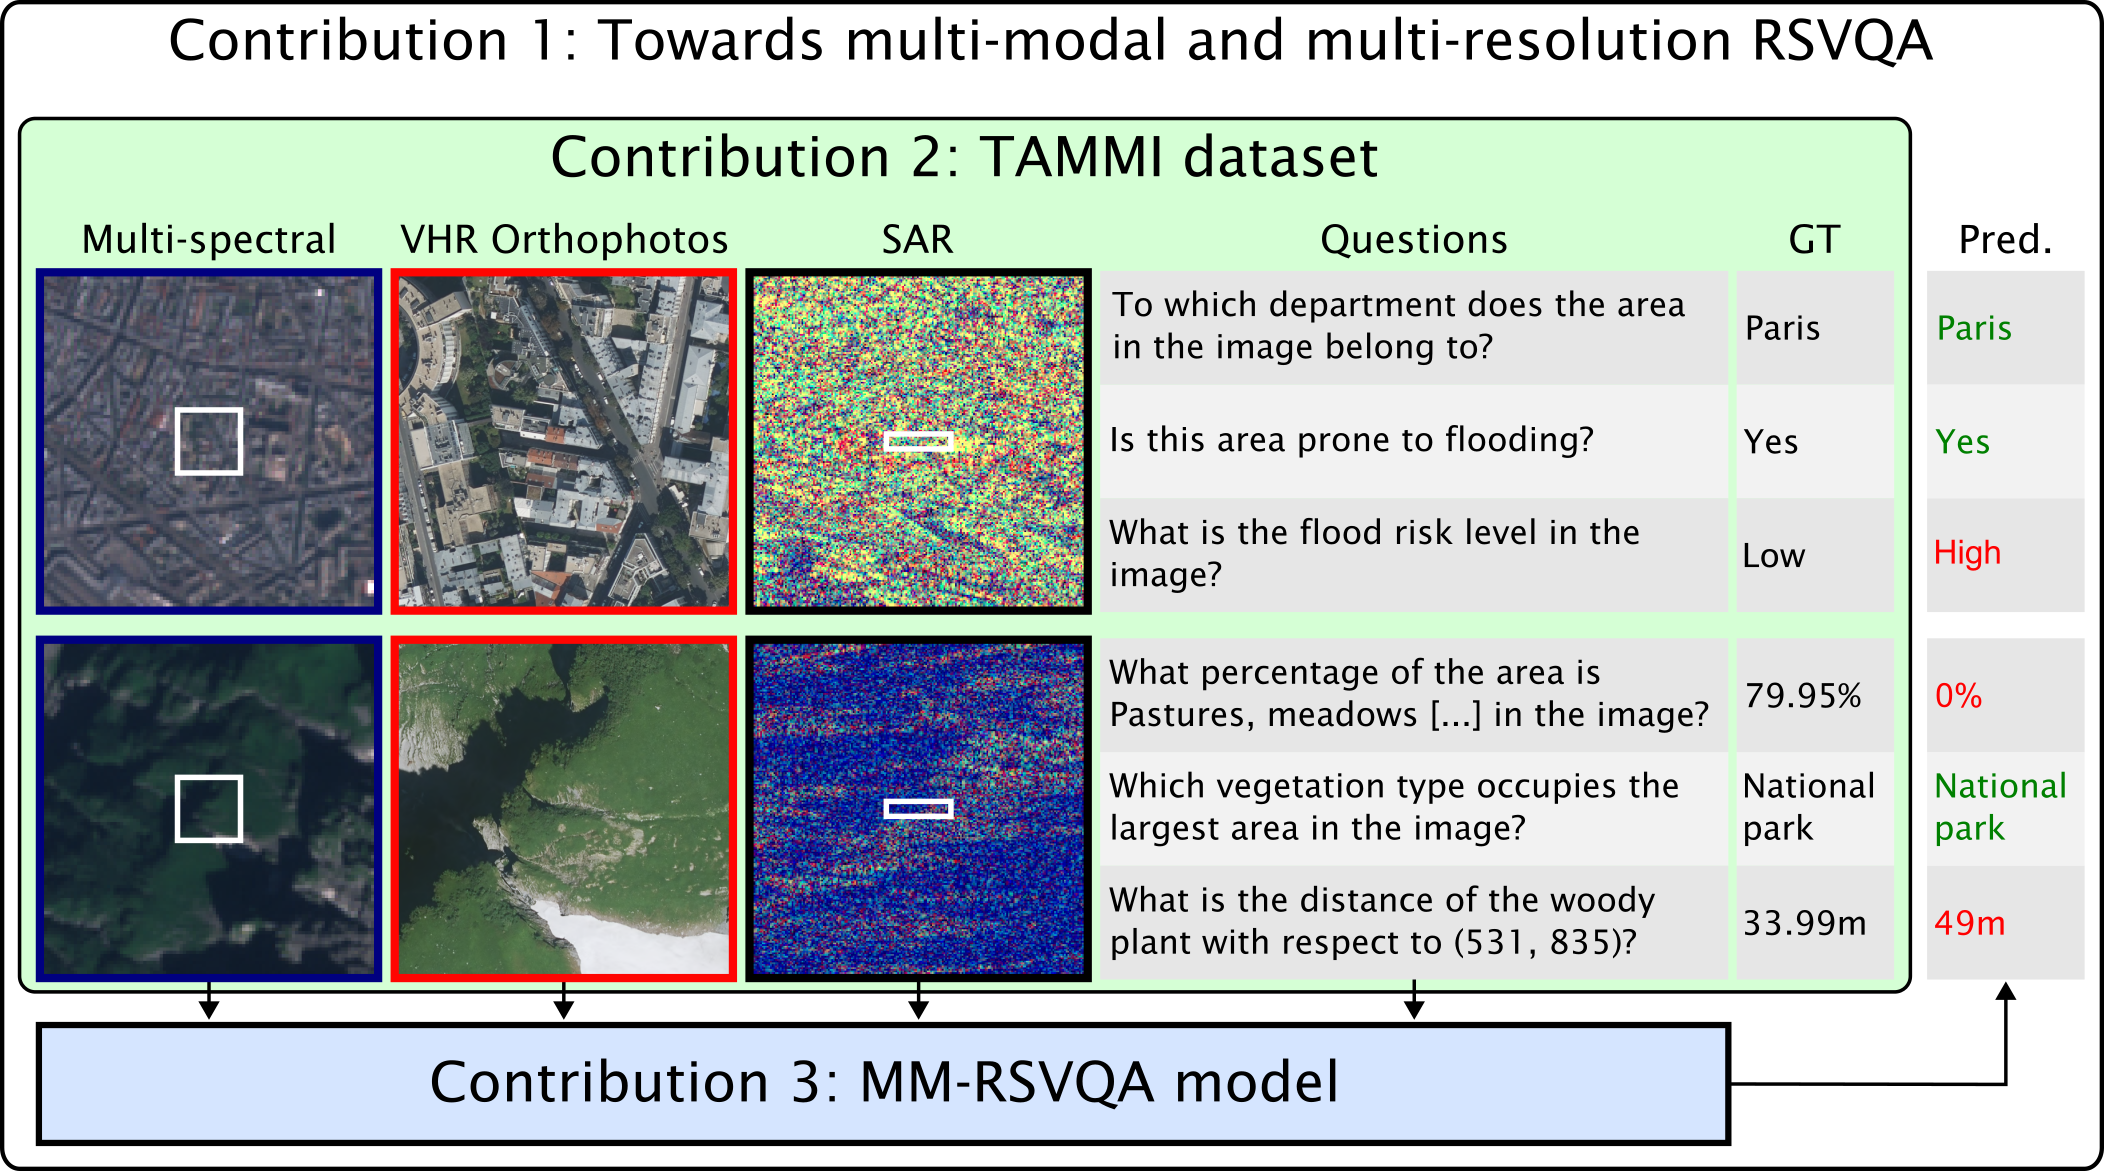
\includegraphics[width=\columnwidth]{images/TAMMI/GraphAbstract.png}
\caption{Summary of our contributions.
We introduce a new task in the computer vision community with multi-modal and multi-resolution Visual Question Answering (VQA) on remote sensing images. 
We introduce a new dataset, TAMMI, associating question/answer pairs to multi-spectral, Very High-Resolution (VHR) orthophotos and Synthetic Aperture Radar (SAR) images triplets. 
In these examples, the white rectangle in the multi-spectral and SAR images corresponds to the extent of the VHR image. 
Finally, we propose a new model for this task referred as MM-RSVQA.}
\label{fig:intro_QA}
\end{figure}


\section{Introduction}
\label{sec:intro}
%\TODO{homogenize everywhere bands versus channels}
%\TODO{when taking about MM-RSVQA, homogenize everywhere architecture versus model versus method}
The task of Visual Question Answering (VQA) aims at providing natural language answers to free-form, open-ended question about an image~\cite{antol2015vqa}. 
On natural images, recent advances in the computer vision and natural language processing communities have shown great improvements to standard VQA benchmarks. %TODO CITE
In particular, Large Language Models (LLM) can now be used to perform knowledge-based VQA, which requires external knowledge and commonsense reasoning~\cite{hu2023promptcap}. 
These models are however more limited when used beyond natural images~\cite{li2023comprehensive, khan2023q}.

VQA has been proposed for the medical domain~\cite{hasan2018overview} and is an active field of research in the medical and computer vision communities~\cite{lin2023medical}. 
The VQA task is also used for extracting information from remote sensing data~\cite{lobry2020rsvqa}. 
In such thematic domains, there are significant challenges compared to VQA for natural images. 
In particular, the limited availability of high-quality training data and the variability of information found in different imaging modalities have been active research topics~\cite{lin2023medical, yuan2023multilingual, khan2023q}.

It is commonly agreed that VQA methods for both of the remote sensing and medical imaging fields would benefit from information contained in different modalities of images~\cite{persello2022deep}. 
Indeed, multiple image modalities are often used in these fields to obtain different, specific and complementary (spectral, spatial and contextual) information about a single scene.
%However, to the best of our knowledge, VQA from multi-modal images have not been explored~\cite{lin2023medical}. 
In remote sensing in particular, multi-modal data allows to obtain different information at multiple resolutions and from various wavelengths, from the 400nm of ultraviolet to the 5cm of radar wave. 
Among others, Very-High Resolution (VHR) data offers images at sub-meter resolutions. 
With Multi-Spectral (MS) data, it is possible to characterize different ground materials thanks to their different spectral responses. 
Synthetic Aperture Radar (SAR) offers imaging capacities highlighting man-made objects and giving physical information about objects~\cite{li2022deep}.
While previous works have explored VQA from multi-modal images \cite{tosato2024can}, using RGB data from the Sentinel-2 satellites and SAR data from Sentinel-1 on existing datasets, dedicated datasets and methods are necessary. 

Our first contribution (highlighted in \autoref{fig:intro_QA}) is to tackle the task of VQA from multi-modal and multi-resolution images leading to a novel challenging task for the computer vision community. 
Our second contribution is a new dataset named TAMMI, built from openly available data sources. 
This dataset combines three modalities (VHR, MS and SAR) and we make it openly available. 
We also share with the vision community an automated pipeline to easily extend this dataset (e.g. to new geographical areas or modalities) according to experimental needs.
%Lower resolution images 
MS and SAR can be used dynamically at different sizes to provide different levels of context. 
Finally, our third contribution is a baseline model for the targeted multi-modal VQA task named MM-RSVQA. 
The proposed architecture is able to take as input the three image modalities, with specifically pre-trained feature extractors. 
To effectively integrate the multi-modal visual features, along with the textual features of the question, we use VisualBERT, a recent vision-language transformer, leading to a trainable fusion scheme. 

\section{Related works}
\label{sec:SoA}
\textbf{VQA} has the objective of predicting a natural language response to an open-ended question related to an image~\cite{antol2015vqa}. 
This task bridges visual reasoning with semantics expressed in natural language, providing new challenges for the computer vision community. 
Models relying on attention~\cite{yang2016stacked, anderson2018bottom, zhou2021trar} to extract relevant features have been proposed. 
Recently, foundation models such as CLIP~\cite{radford2021learning} have shown remarkable success on the VQA downstream task~\cite{shen2021much}.
However, such approaches do not translate directly to thematic applications of the VQA task~\cite{eslami2023pubmedclip}.

The task of VQA for remote sensing (RSVQA) is introduced in~\cite{lobry2020rsvqa}. 
In this work, features are extracted using a Convolution Neural Network (CNN) and a Recursive Neural Network (RNN) and fused together with a point-wise multiplication. 
Improvements in the feature extractor have been proposed by Felix et al.~\cite{felix2021cross}, inspired by LXMERT~\cite{tan2019lxmert} enhancing the results using an object detection step implemented via the Faster-RCNN model as a visual encoder and BERT for the language part. 
%In this work, the authors propose two datasets for the task. A simple baseline using a pre-trained ResNet-152~\cite{he2016deep} to encode the image and a pre-trained skip-thoughts vectors~\cite{kiros2015skip} to extract the text representations is proposed. The representations are then projected into a common space via a fully connected layer using a fusion mechanism based on point-wise multiplication. The task is treated as a classification problem, with a multi-layer perceptron to predict the answer.
The Fourier transform is also used in~\cite{zhaofrequency} to extract structural information from complex remote sensing data, thereby improving the generalizability across various domains.
In~\cite{chappuis2023multi}, an object detector and a classifier are used to create a caption of the image, then used to answer the question. 
LLMs such as BERT~\cite{devlin2018bert} have been used for textual features extraction~\cite{chappuis2022language} or as the main component of the model~\cite{chappuis2022prompt}. 
The fusion step of the two representations is done in~\cite{felix2021cross} with a cross-modal transformer encoder. 
Another attention-based method is proposed in~\cite{zheng2021mutual}, with a fusion module based on mutual attention. 
In~\cite{tosato2024segmentation}, a method that uses segmentation maps to guide the attention is introduced. 
In parallel, training techniques such as self-supervised curriculum learning~\cite{yuan2021self} have been shown to be efficient to obtain a common representation of textual and visual features. 
Improvements to the language processing have been introduced as well: in~\cite{yuan2023multilingual} an augmentation is applied to translate each question in multiple languages and then translate it back to English, improving the diversity of the formulation of questions. 
%This generator produces a textual description of the image, which is then used in a DistilBERT~\cite{sanh2019distilbert} language model as a context along the question.

\noindent\textbf{Datasets} Several datasets have been created for RSVQA. 
This problem is first considered in~\cite{lobry2020rsvqa} which introduced two RSVQA datasets composed of image/question/answer triplets. 
The first one, called "Low Resolution (LR)", is based on images from the Sentinel-2 sensors (optical images with a spatial resolution of 10m) acquired over The Netherlands. 
The second one, called "High Resolution (HR)", uses RGB aerial images with a spatial resolution of 15cm extracted from the USGS High Resolution Orthoimagery database, covering urban areas of the United States. 
In these two datasets, the nature of the questions, as well as the distribution of answers, is highly unbalanced (e.g. ’0’ in the HR dataset has a frequency of 60.9\% for the numerical answer). 
In addition, the number of different answers is very limited, with 9 possible answers for LR and 98 for HR. 
RSVQAxBEN~\cite{lobry2021rsvqa} dataset proposes a larger number of samples and introduces new objects of interest (land cover classes) with a new form of complexity (logical formulas). 
The area of interest is also different, as it covers many European countries thanks to images from the Sentinel-2 satellites.  
However, even in this dataset, the imbalance in the distribution of answers remains. 
In order to increase the diversity of questions, Zheng et al.~\cite{zheng2021mutual} have exploited five pre-annotated datasets, three for scene classification and two for object detection for the automatic construction of questions and answers.

These datasets have certain limitations in common. 
First, most of them have a limited number of samples, which may reduce the ability of deep learning models to generalise effectively~\cite{lobry2020rsvqa}. 
In addition, the diversity of questions and answers is often restricted, which can lead to biases and gaps in model performances~\cite{chappuis2023curse}. 
Finally, these datasets focus on the use of RGB images, not leveraging other modalities, sensors and resolutions.

%In general, the integration of SAR images with natural language has been under-explored and seems to be a challenging area due to the inherent complexity and unique data structure of SAR imagery. 
%Deep learning models often struggle with SAR-based tasks that require precise quantification, such as estimating the size of targets or counting objects~\cite{zhao2022exploring}.
%However, these models are effective in tasks focused on spatial relationships, such as identifying the proximity of objects or providing density assessment within SAR scenes. 
%SAR has also been introduced as the main modality into RSVQA for specific tasks such as scattering patterns classification~\cite{aghababaei2024visual}, ships detection and counting~\cite{wang2024visual} and fused with optical images to answer questions related to the land cover~\cite{tosato2024can}.
Integrating SAR imagery with natural language remains under-explored and challenging due to its unique data structure. Deep learning models often struggle with SAR-based tasks requiring precise quantification, such as target size estimation or object counting~\cite{zhao2022exploring}. However, they are effective in tasks involving spatial relationships, like proximity identification or density assessment within SAR scenes. SAR has been used in RSVQA for tasks such as scattering pattern classification~\cite{aghababaei2024visual}, ship detection and counting~\cite{wang2024visual}, and in combination with optical images for land cover related questions~\cite{tosato2024can}.

%The limited consideration of the SAR modality has constrained its full integration into RSVQA datasets, ending up restricting the domains in which a dataset can be utilized and the depth of the study that can be applied to the researches based on them. Having access to different modalities also require merging information in the best possible way. 
%The most common fusion techniques are early fusion~\cite{sumbul2019bigearthnet}, halfway fusion~\cite{boulahia2021early} and late fusion~\cite{chen2023efcomff}. 
%Over the past decade, however, the fusion technique that has been increasingly used is transformers, for classification~\cite{roy2023multimodal}, object detection~\cite{bai2022transfusion} and segmentation~\cite{zhang2022mmformer}. 

In this work, beyond sharing a new vision task with the community, we address existing gaps in the current state of the art by creating a diverse dataset that spans multiple complementary image modalities, resolutions, and geographic regions, encompassing a wide range of terrain types and incorporating various question typologies. 
As a first baseline on this task and dataset, we embed state of the art transformer-based fusion techniques proven effective through a new model for tackling multi-modal challenges.

%In~\cite{zhang2019cross}, the three methods were compared showing that halfway fusion seems to have better results than the other two. 



\section{Dataset}
\label{sec:dataset}
For the purpose of advancing RSVQA capabilities we develop TAMMI (\textit{Text and Multi-Modal Imagery}), a large multi-modal and multi-resolution dataset. 
TAMMI includes images/question/answer triplets on three French departments, shown in \autoref{fig:GeoExtent}. 
The following subsections outline each phase of the dataset creation, detailing data sources and processing steps involved.


\subsection{Image modalities}
\paragraph{Very high-resolution orthophotos (BDOrtho)}
BDOrtho is a dataset of aerial VHR optical images acquired by the french National Geographic Institute (IGN). 
It provides an accurate and detailed photographic representation of the French territory at 20cm resolution. Images are provided in RGB and updated every three years. For our dataset, the most recent images are chosen for each department: images from department 74 are from 2020, and images for department 34, 75, 92, 93, 94 are from 2021. 
To ensure consistency in the information provided by the images, the same years are maintained for the images of the other modalities.

\paragraph{Multi-spectral data (Sentinel-2)}
Sentinel-2 is a mission of the European Union's Copernicus program, designed to provide multi-spectral images of land. 
Sentinel-2 captures data in 13 bands of the electromagnetic spectrum~\cite{S2mission}, including near-infrared (NIR), visible and short-wave infrared (SWIR) with a spatial resolution of 10m, 20m, or 60m depending on the band. 
Sentinel-2 images are acquired every five days when both Sentinel-2A and Sentinel-2B are active. 
The images are distributed as Level-1C (L1C) products which provide top-of-atmosphere (TOA) reflectance, and Level-2A (L2A) that offer surface reflectance after atmospheric correction. 
Since our dataset includes SAR images which are not affected by atmospheric conditions and BDOrtho images which are taken during sunny days and do not need any atmospheric correction, we select L1C products. 
Furthermore, only images with a cloud coverage under 3\% are selected. 

\if 0 
\begin{table}[!t] \centering 
\begin{tabular}{lcc}
        \hline
        \textbf{Bands} & \textbf{WL (nm)} & \textbf{Res. (m)} \\
        \hline
        B1 - Coastal aerosol  & 443            & 60 \\\hline
        B2 - Blue& 490            & 10   \\\hline
        B3 - Green  & 560            & 10  \\\hline
        B4 - Red & 665            & 10  \\\hline
        B5 - Vegetation Red Edge & 705            & 20   \\\hline
        B6 - Vegetation Red Edge & 740            & 20  \\\hline
        B7 - Vegetation Red Edge & 783            & 20 \\\hline
        B8 - NIR & 842            & 10  \\\hline
        B8A - Vegetation Red Edge  & 865            & 20 \\\hline
        B9 - Water Vapour  & 945            & 60\\\hline
        B10 - SWIR - Cirrus  & 1375           & 60  \\\hline
        B11 - SWIR & 1610           & 20  \\\hline
        B12 - SWIR & 2190           & 20 \\
        \hline
    \end{tabular} 
    \caption{Spectral bands of the Sentinel-2 optical sensors 
    (WL: wavelength, Res.: spatial resolution, NIR: Near Infra-Red and SWIR: Short Wave Infra-Red).} 
    \label{tab:S2Bands}
\end{table}
\fi  
%\textcolor{red}{Give additional details, maybe table with all bands?}

\paragraph{Synthetic Aperture Radar data (Sentinel-1)}
The Sentinel-1 satellite is also part of the European Union's Copernicus program,  designed to provide full coverage of Europe every 6 days.
Sentinel-1 acquires SAR images by sending radar pulses towards the earth's surface and measuring the backscattered signal. 
Since the radar pulses propagate through clouds, the acquisition rate is independent of the atmospheric conditions. 
%Sentinel-1 images are distributed with three levels of processing, the first one represents the raw data, the second involves the calibration and initial processing, and the last includes further refinement and enhancement of the data to generate specialized products for specific applications.
In our dataset, we use Interferometric Wide (IW) swath mode. IW is the main acquisition mode over land and has a resolution of 5m in range (across satellite trajectory) and 20m in azimuth (along trajectory).
In this acquisition mode, the swath is divided in three sub-swathes. 
The satellite acquires tiles, called \textit{burst}, in each sub-swath sequentially with an overlap between the bursts. 
The bursts are processed as separate Single Look Complex (SLC) images. In the Sentinel-1 SLC products, sequentially acquired bursts of the same sub-swath are included into a single image separated by black bands.
Sentinel-1 acquires data in two polarization channels (VV and VH), providing additional information about the characteristics of materials on the planet surface.
In this work, we use the amplitude of the SLC level 1 images for both polarization channels.

%\Lu{i have to add 'SAR images are acquired by a sensor laterally with respect to the direction of the satellite. A signal impulse of varying frequency is sent, and its return signal, called backscattering, is saved.'}

\begin{figure}[!t]
\centering
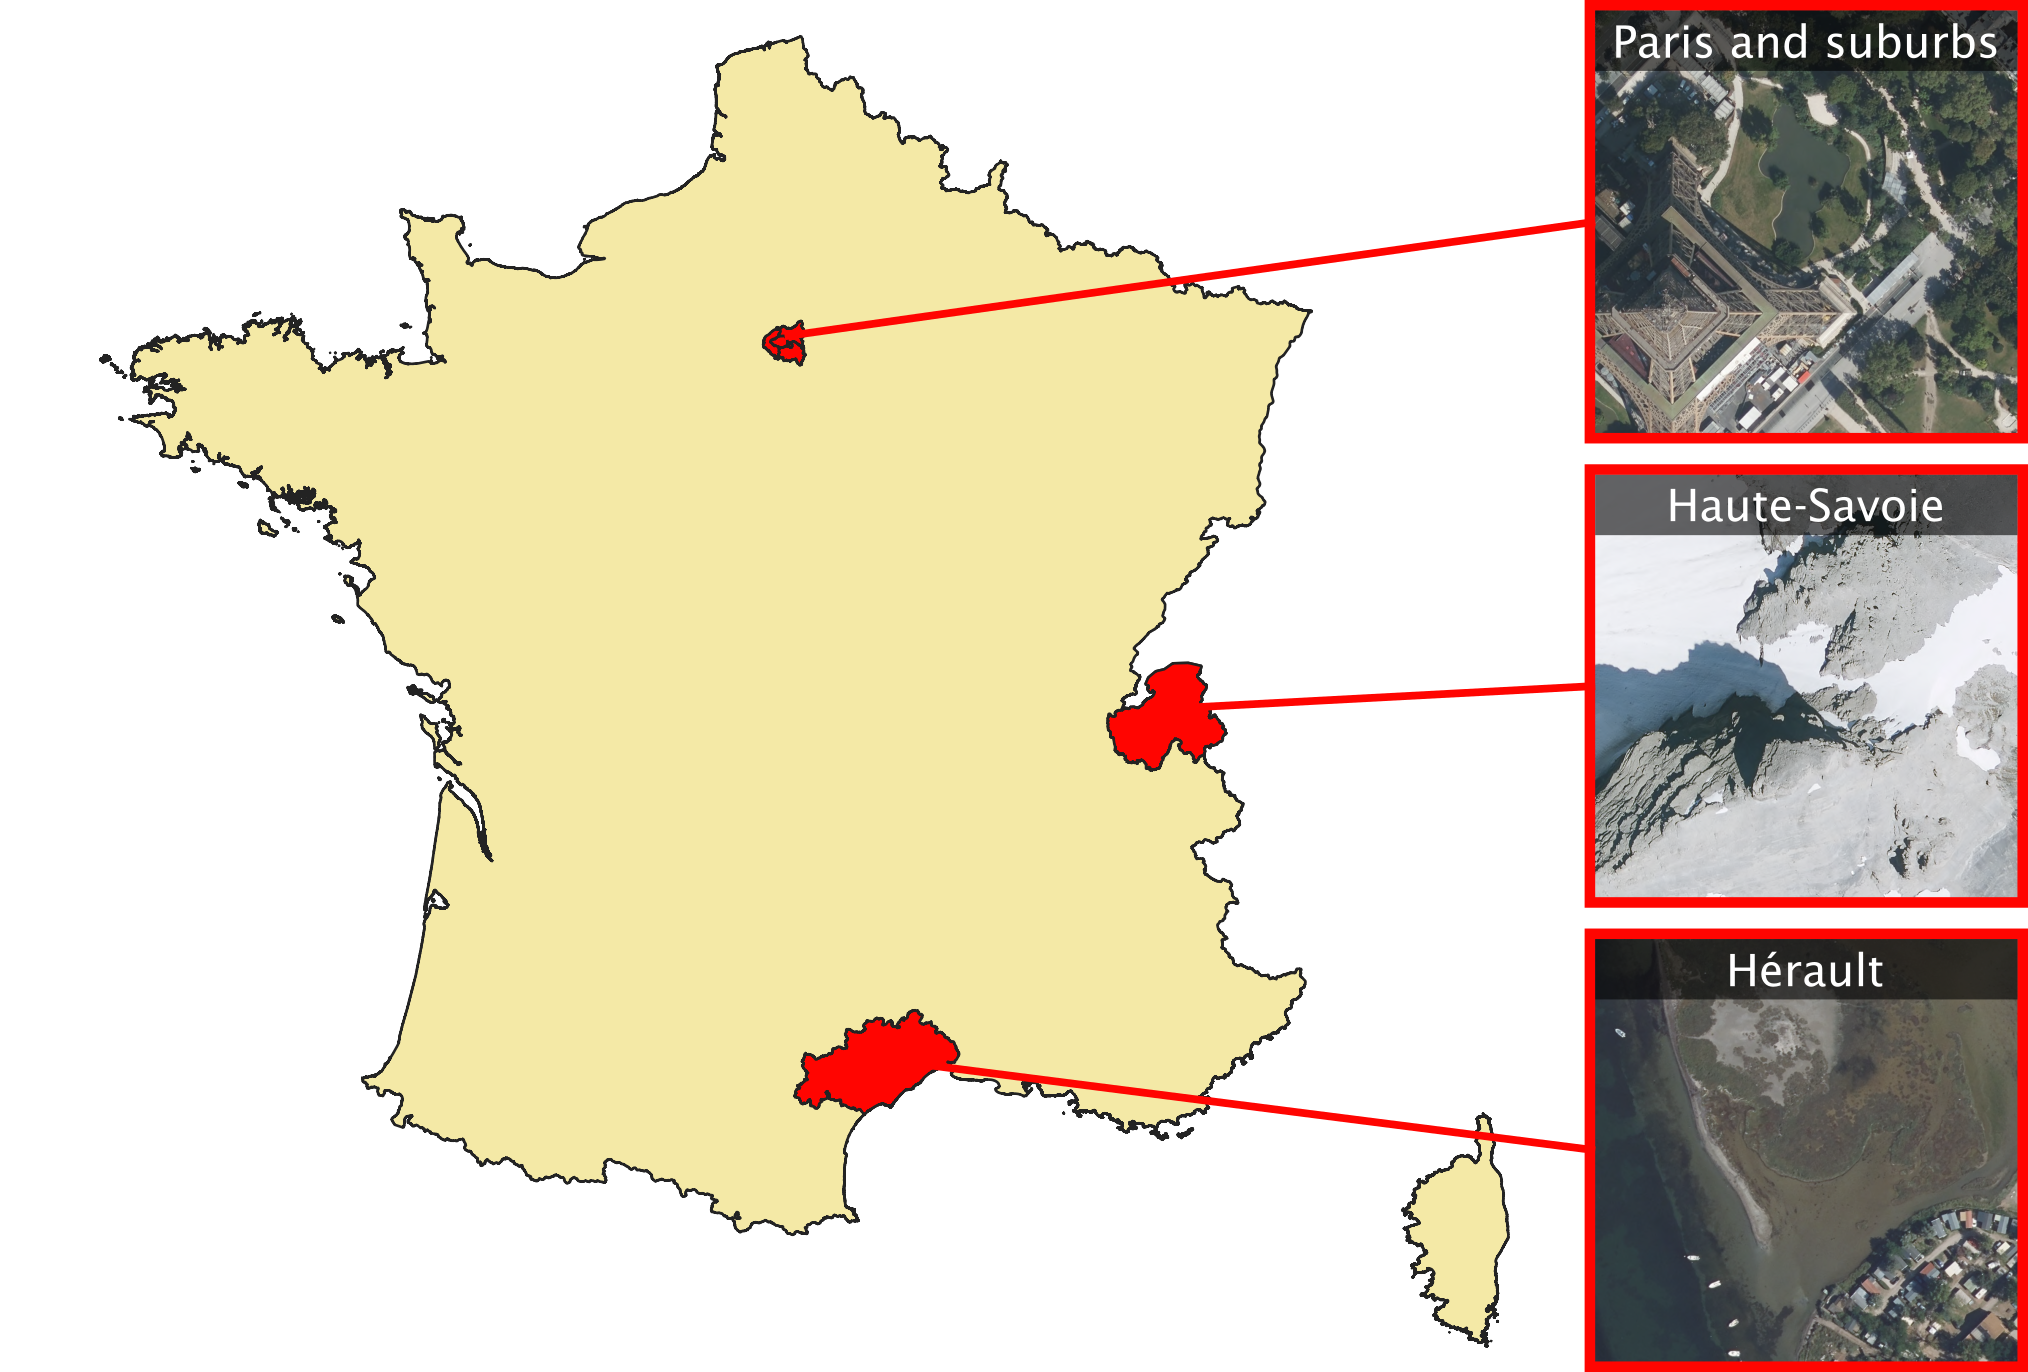
\includegraphics[width=\columnwidth]{images/TAMMI/GeoExtent.png}
\caption{Geographical extent of the TAMMI dataset, covering selected regions (highlighted in \textcolor{red}{red}) in Metropolitan France: 
Paris and inner suburbs (departments 75, 92, 93, 94), an urban region; 
Haute-Savoie (74), a mountainous region; 
and Hérault (34), a seaside region. 
For each of these regions, we show a VHR sample from the dataset.}
\label{fig:GeoExtent}
\end{figure}

\subsection{Image triplets}
To build the question/answer parirs, we select the geographical extent of the VHR patches $\pvhr$. The VHR patches are extracted from the division of the VHR tiles (of dimension 25000 $\times$ 25000 pixels) of our areas of interest (shown in \autoref{fig:GeoExtent}) into patches of size 1000 $\times$ 1000 pixels (i.e. 200m $\times$ 200m). The areas of interest are selected for their diverse landscapes. Specifically, the Île-de-France region (departments 75, 92, 93, 94) is predominantly urban, while the Haute-Savoie region (department 74) features mountainous terrain, and the Hérault region (department 34) is maritime. 
Since MS ($\pms$) and SAR ($\psar$) patches are designed to offer spatial context to the model, their extent (respectively $\lms$ and $\lsar$) is defined by the user and the patches are cropped at execution time. 
To align the images of all three modalities, we retrieve the latitude, longitude and altitude of the central pixel for each VHR patch. 
We then associate a MS and a SAR tile centered on the position of the central pixel of the VHR patch. 
The MS tiles are geocoded. Therefore, the latitude and longitude are converted to the image pixel space.
For SAR images, we use the method of~\cite{Weissgerber2022} to project the position of the central pixel of $\pvhr$.
To produce continuous SAR patches, the SAR images are debursted (removing black lines and burst overlaps), and pre-processed with tail-value removal based on histogram analysis for each polarization, then a transformation to decibels and a normalization are applied. The pre-processing steps are detailed in the supplementary materials.

\if 0
\paragraph{Sentinel-2} 
As far as Sentinel-2 is concerned, once latitude and longitude are converted from terrestrial coordinates to Sentinel-2 coordinates, new center pixel values for the image are calculated. 
The center pixel value is saved in the final JSON splits, so the user can choose the patch size to be used, the programme will use the centre of the patch to retrieve the correct portion of the image.
\paragraph{Sentinel-1} 
The first difference to take into account with respect to optical images is that in Sentinel-1's images, using IW mode and SLC level 1, they are divided into bursts by black lines and repeated areas. For this reason, we must be sure not to select part of the black image during patch cropping as shown in Figure~\ref{SARimagesprepost}. To achieve this, the black lines and repeating zones are removed, following the procedure below:
\begin{itemize}
    \item the energy present for each line of the image was calculated
    \item the average of the energies was calculated
    \item if the energy of a line is less than the average energy divided by 1.5, the line is considered black.
    \item rows in the vicinity of the black ones just identified are compared to see if they are equal. 
    \item Equal rows above the black line are eliminated, as there is no repetition in the final image. 
\end{itemize}

 \begin{figure}[t!]
    \centering
    \begin{subfigure}[b]{0.49\columnwidth}
        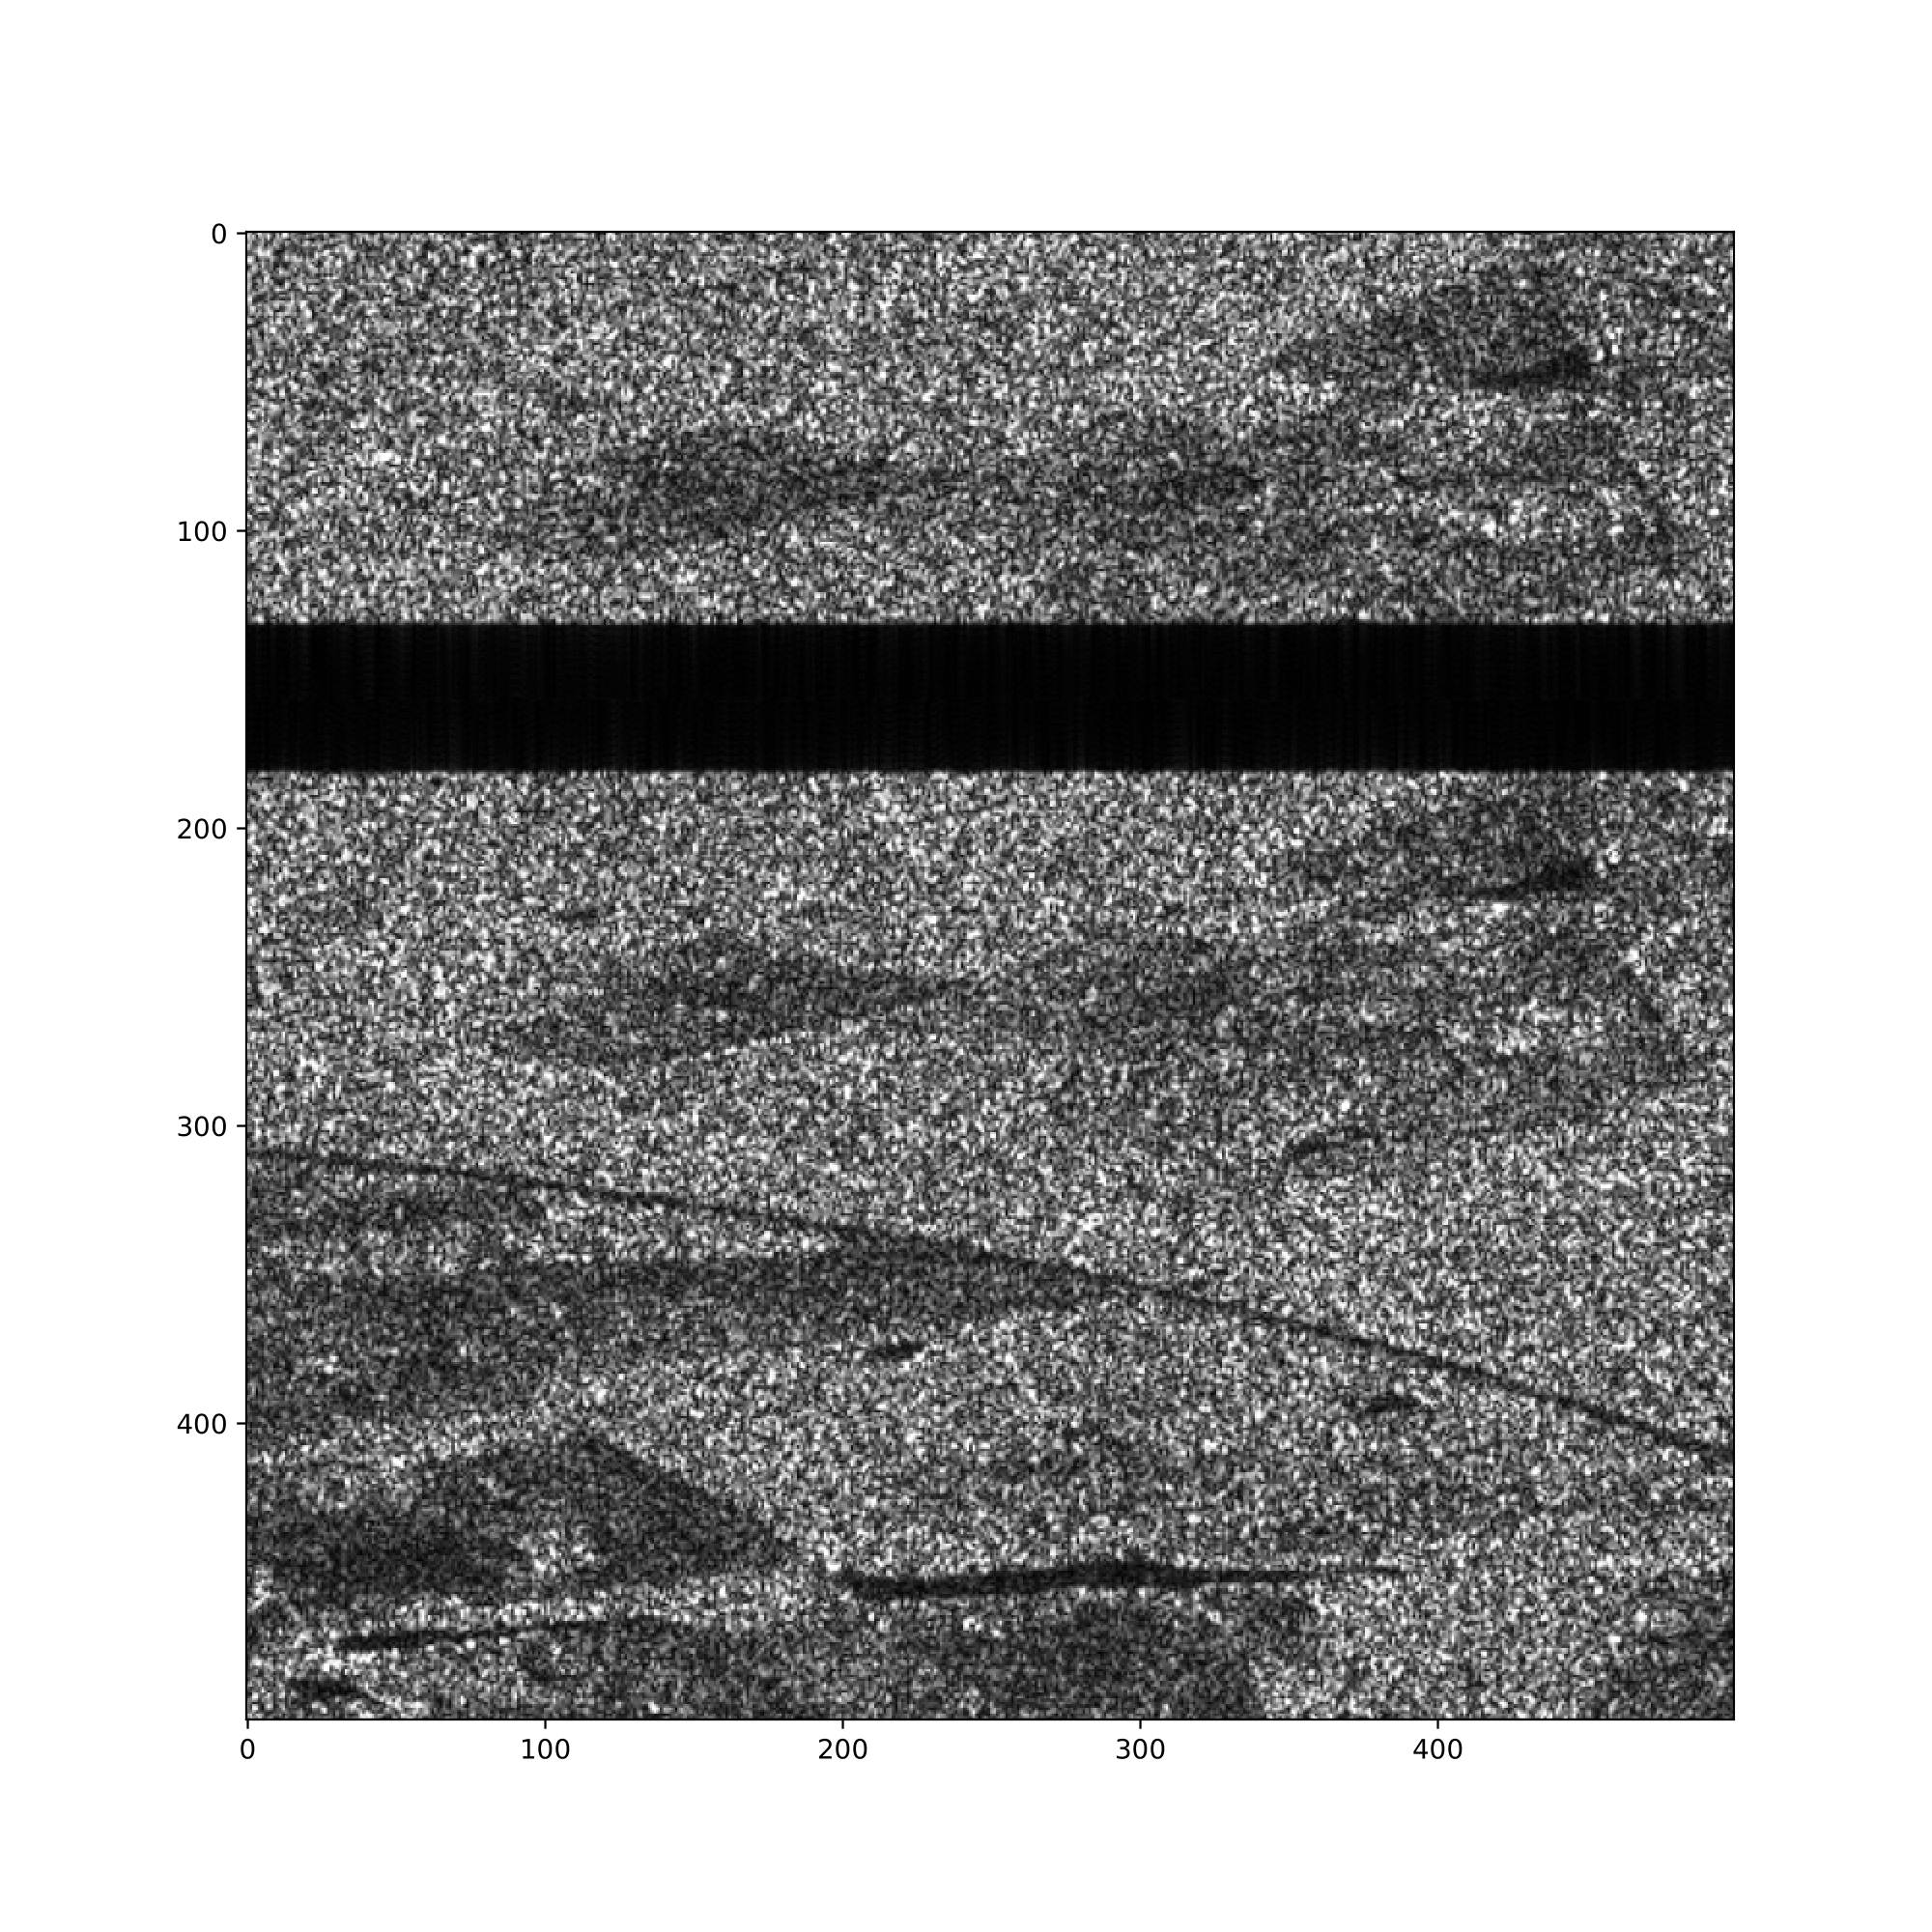
\includegraphics[width=\columnwidth]{images/TAMMI/original_patch.pdf}
        \caption{Pre}
        \label{fig:image_a}
    \end{subfigure}
    \begin{subfigure}[b]{0.49\columnwidth}
        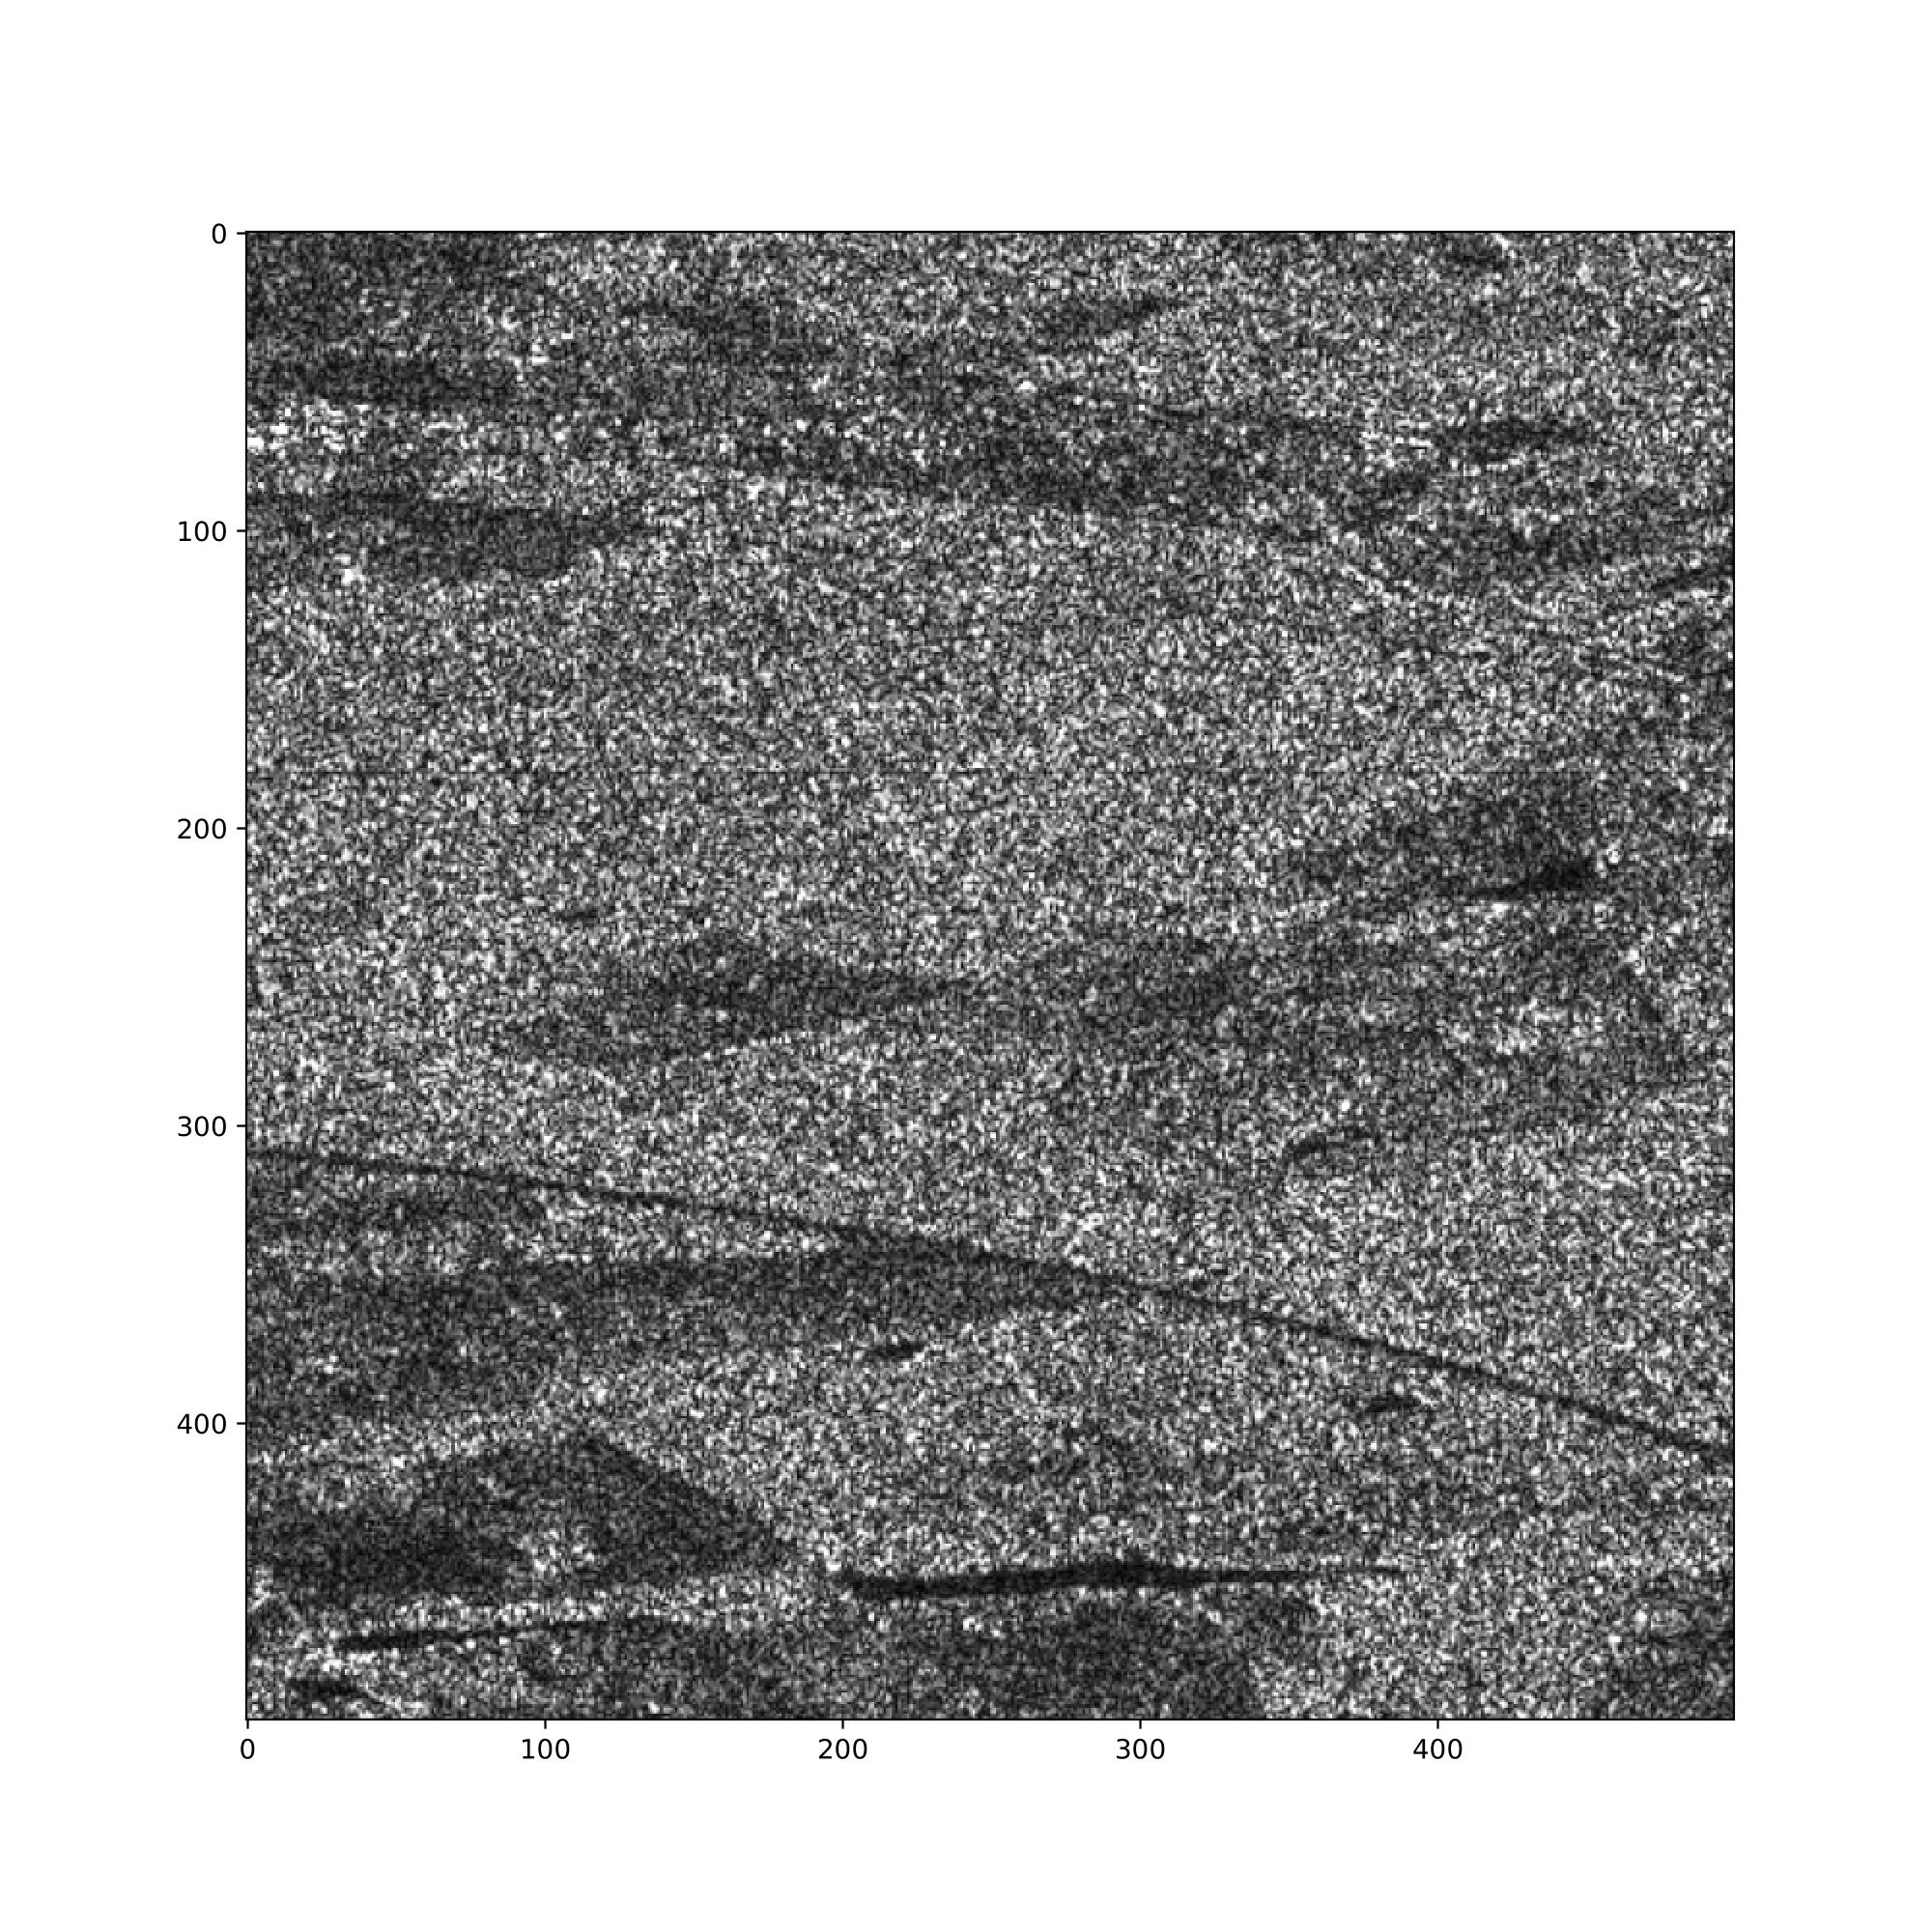
\includegraphics[width=\columnwidth]{images/TAMMI/final_patch.pdf}
        \caption{Post}
        \label{fig:image_b}
    \end{subfigure}
    \caption{SAR image patch extraction}\label{SARimagesprepost}
\end{figure}
The way SAR images are acquired also creates geometric distortions such as foreshortening, layover, and shadow. Layover in SAR images is caused by high objects, making them appear closer to the sensor with respect to other objects. This happens because the backscattering signal returns faster to the sensor, as it has to travel a shorter distance due to the high height of the objects. It is the reason why it is not possible to calculate the coordinates of the associated pixel directly from the latitude and longitude of a point. \\
\fi  


\subsection{Question/answer pairs}
%Inspired by \cite{johnson2017clevr}, we propose an automatic method for the construction of question/answer pairs associated to each VHR patch, using:
Inspired by \cite{johnson2017clevr}, we propose an automatic approach for the construction of question/answer pairs associated to each geographical area covered by the VHR patch, using: 
\begin{itemize}
    \item \textbf{BDTopo} provided by IGN (French Geographical Institute). It is an official vectorial description of the French territory, including generic geographical objects (e.g. buildings and water areas), and specific ones (e.g. museums and lakes);
    
    \item \textbf{Flooding risks database (TRI)} from \textit{Géorisques}. This dataset corresponds to the areas at significant risk of flooding, including management zoning, floodable area zoning, water level zoning, etc.;
    
    \item \textbf{Urban units 2020 (BU20)} of INSEE (French National Institute of Statistics and Economic Studies). This database corresponds to the urban zoning of French cities according to the continuity of the constructions and the number of inhabitants;
    
    \item \textbf{CORINE Land Cover (CLC) 2018} produced as part of the Copernicus European land monitoring program and managed by the European environment agency. It is a database of land cover and land use classifications, on three different levels of hierarchy with different levels of details. 
    In this work, we consider the Level-3 having the most detailed classes (44);
    
    \item \textbf{European Mountain Areas (EMA)} provided by the European environment agency. It contains information about the geometry, the area and the name of the mountains in Europe.
\end{itemize}

\paragraph{Construction of questions}
For a given VHR patch $\pvhr$, we retrieve the collection of geo-located objects $\objects$ that are present in $\epvhr$, the geographical extent of $\pvhr$.
A collection of objects $\mathbf{\objects_{\class}} = \{\objects^{\class}_{i}\}$  are characterised by a class $\class$. A class is one element present in BDTopo, TRI, CLC, EMA, or an Urban Unit. We define five question types that can be divided into 21 sub-questions: %We define 21 questions types that can be divided in five categories:
\begin{enumerate}
    \item \textbf{Presence Questions}: questions about the existence of certain objects or features in the image. 
    \begin{enumerate}
        \item \textbf{Presence}: answered with \textit{yes} if the cardinality of the set of object from the class $\numobj > 0$ and \textit{no} otherwise, where $\class \in$ BDTopo, \\e.g. \underline{"Is there a road in the image?"}
        \item \textbf{Mountain presence}  answered with \textit{yes} if the cardinality of the set of object from EMA $\numobj > 0$ and \textit{no} otherwise, \\e.g. \underline{"Are there any mountains in the image?"}
        \item \textbf{Flood presence}  answered with \textit{yes} if the cardinality of the set of objects from TRI $\numobj > 0$ and \textit{no} otherwise, e.g. \underline{"Is this area prone to flooding?"}
    \end{enumerate}

    \item \textbf{Quantity Questions}: questions about the number or amount of certain objects or features in the image.
    \begin{enumerate}
        \item \textbf{Count}: answered by $\numobj$, where $\class \in$ BDTopo, \\e.g. \underline{ "How many buildings are in the image?"}
        \item \textbf{Density} answered by $\frac{(\sum_{i=1}^{\numobj} a(\objects^{\class}_{i})) \times 100}{a(\pvhr)}$ where $a(.)$ is a function returning the area, and $\class \in$ BDTopo , \\ e.g. \underline{ "What is the religious buildings density?"}
        \item \textbf{Area}: answered by $a(\objects^{\class}_{i})$,  where $\class \in$ BDTopo ,\\ e.g. \underline{ "What is the area of the lake?"}
        \item \textbf{Percentage}: answered by $\frac{(\sum_{i=1}^{\numobj} a(\objects^{\class}_{i})) \times 100}{a(\pvhr)} $ where $\class \in$ CLC,\\ e.g. \underline{ "What percentage of the area is wetland?"}
    \end{enumerate}

    \item \textbf{Location Questions}: questions about the location of certain objects or features in the image.
    \begin{enumerate}
        \item \textbf{Absolute location}: answered by $\textrm{loc}(\objects^{\class}_{i})$ where $\textrm{loc}(.)$ is a function returning the position (both as the exact coordinate in the image space, and as the position in a $3\times 3$ grid dividing the image) of a specific object, and $\class \in$ BDTopo, \\e.g. \underline{ "Where is the largest vegetation area?"}
    \end{enumerate}


    \item \textbf{Classification Questions}: questions about the classification or type of certain objects or features in the image.
    \begin{enumerate}
        \item \textbf{Water bodies}: answered by the class $\class$ of $\max a(\objects^\class)$ or $\min a(\objects^\class)$,  where $\class \in$ BDTopo's water category (see appendix), \\e.g. \underline{ "What type of water body occupies the largest}\\ \underline{area in the image?"}
        \item \textbf{Vegetation zones} answered by the class $\class$ of $\max a(\objects^\class)$ or $\min a(\objects^\class)$,  where $\class \in$ BDTopo's vegetation category (see appendix),\\ e.g. \underline{ "Which vegetation type occupies the smallest}\\ \underline{area in the image?"}
        \item \textbf{Mountain range name}: asked only if the answer of mountain presence is \textit{yes}, and answered by $n(\objects_{i})$ where $n(.)$ is a function returning the name of the mountain range present in the geographical extent of $\pvhr$,\\ e.g. \underline{ "What is the name of the mountain range in the}\\ \underline{image?"}
        \item \textbf{Flood level}: answered by $\textrm{flood}(\epvhr)$ where $\textrm{flood}(.)$ is a function returning the highest flood risk present in $\pvhr$. The possible answers of this function are ‘low’, ‘medium’, and ‘high’. \\e.g. \underline{ "What is the flood risk level?"}
        \item \textbf{Flood type}: answered by $\textrm{type}(\epvhr)$ where $\textrm{type}(.)$ is a function returning all types of flood risks present in $\pvhr$. The possible answers of this function are 'River overflows', 'Runoff', 'Sea Flooding' and 'GroundWater overflows' \\e.g. \underline{ "What is the nature of the flood risk in this}\\ \underline{ area?"}
        \item \textbf{Land cover}: answered by the CLC class with the largest (or smallest) area,\\ e.g. \underline{ "Which land cover category occupies the}\\ \underline{largest area in the image?"}
        \item \textbf{Urban }: answered by $\textrm{urban}(\epvhr)$ where $\textrm{urban}(.)$ is a function returning the urban classification (City Center, Suburb, Isolated City, Outside Urban Unit) based on BU20,\\ e.g. \underline{ "What is the urban classification of the area}\\ \underline{in the image?"}
        \item \textbf{Department}: answered by $\textrm{dpt}(\epvhr)$ where $\textrm{dpt}(.)$ is a function returning the name of the departement of $\epvhr$, \\e.g. \underline{ "To which department does the area in the} \\\underline{image belong to?"}
        \item \textbf{Region}: answered by $\textrm{reg}(\epvhr)$ where $\textrm{reg}(.)$ is a function returning the name of the region of $\epvhr$,\\ e.g. \underline{ "To which region does the area in the image}\\\underline{belong to?"}
    \end{enumerate}

    \item \textbf{Relational Analysis Questions}:
    questions seeking to understand the relationships, comparisons, and distances between various objects or features in the image (note that for theses questions $\class \in$ BDTopo).
    \begin{enumerate}
        \item \textbf{Distance}: answered by $d(\objects^{\class_1}_{i}, \objects^{\class_2}_{j})$ where $d(.,.)$ is a function returning the distance (in meters) between two objects (note that $\objects^{\class_1}_{i}$ can be replaced by a position $\textrm{pos}$),\\ e.g. \underline{ "What is the distance between the museum}\\ \underline{and the religious place?"}
         \item \textbf{Comparison}: answered with \textit{yes} if $|\mathbf{\objects_{\class_1}}| > |\mathbf{\objects_{\class_2}}|$, \textit{no} otherwise, \\e.g. \underline{ "Are there more buildings than roads?"}
         \item \textbf{Relative location}: answered by $l^{\objects^{\class_1}_{i}}(\objects^{\class_2}_{j})$ where $l^{\objects^{\class_1}_{i}}(.)$ is a function returning the position (both as the exact coordinate in the image space, and as the position in a slice of a regular octagon) of an object with respect to $\objects^{\class_1}_{i}$,\\ e.g. \underline{ "What is the relative position of the}\\ \underline{monument with respect to the river?"}
        \item \textbf{Nearest}: answered by $l_{\textrm{pos}} (\mathbf{\objects_{\class}})$ where $l_{\textrm{pos}}(.)$ is a function returning the position (both as the exact coordinate in the image space, and as the position in a $3\times 3$ grid dividing the image) of the nearest element of a collection from the position $\textrm{pos}$,\\ e.g. \underline{ "Where is the closest road to (142, 221)?"}
    \end{enumerate}
\end{enumerate}

\begin{table*}[!t]
    \centering
    \footnotesize
    \begin{tabular}{cccccccc}
        \hline
        \textbf{Name} & \textbf{Modalities} & \textbf{Resolution} & \textbf{Annotation}& \textbf{\# Images} & \textbf{\# Questions} & \textbf{\# Q. Types} & \textbf{\# Unique A.}\\
        \hline
        TAMMI & 
        \begin{tabular}{c}BDOrtho \\ S2 - MS 10 channels \\ S1 - VV/VH/Ratio channels \end{tabular} 
        & 
        \begin{tabular}{c}0.2m \\ 10-20m \\ $5\times 20$m \end{tabular} 
        & 
        \begin{tabular}{c}  BDTopo, \\ TRI, BU20, \\ CLC, EMA \end{tabular} &
         282'852 & 3'162'514 & 21 & 109'737 
        \\ \hline
        RSVQAxBEN~\cite{lobry2021rsvqa} & S2 - RGB & 10m & BigEarthNet \cite{sumbul2019bigearthnet} & 590'326 & 14'758'150 & 2 & 26’875\\ \hline
        RSIVQA~\cite{zheng2021mutual}  & Various RGB & 0.15–8m & Manual/Other & 37'264 & 111'134 & 4 & 579  \\ \hline
        RSVQA LR~\cite{lobry2020rsvqa} & S2 - RGB & 10m & OSM & 772 & 77'232 & 4 & 9 \\ \hline
        RSVQA HR~\cite{lobry2020rsvqa} & USGS Ortho & 0.15m & OSM & 10'659 & 1'066'316 & 4 & 55\\
        \hline
    \end{tabular}
    \caption{Summary of existing RSVQA datasets, showing modalities (S1: Sentinel-1, S2: Sentinel-2), spatial resolutions, annotation sources, and dataset sizes by image and question counts.} \label{tab:Overview}
\end{table*}



\paragraph{Balancing the dataset}
One of the challenges of constructing a VQA dataset stochastically is to balance both question types and the answer types to reduce language biases~\cite{goyal2017making}.
In this work, we perform the balancing jointly at the dataset and department levels.

We perform the questions/answers pairs construction at the department level. For each VHR patch $\pvhr$ 10 questions per type are randomly constructed. We iterate through the questions created for each patch, and select questions based on four goals: 
1) having an equal number of questions for each type; 
2) having a number of question proportional to the number of VHR patches per department; 3) having a balanced distribution of answers for each type of question; 
and 4) not having more than 50 question/answer pairs for each patch.

In the case of question types with a fixed number of possible answers $\numAnswers$ such as Presence (e.g. Yes/No, $\numAnswers = 2$), the number of questions per answer is defined as 
$\numQuestionsAnswers = \frac{\numPatches}{\min(\numAnswers,10)}$, where $\numPatches$ is the number of patches in the department.
For Location questions, the locations are binned in the $3 \times{} 3$ square grid, leading to $\numAnswers=9$. 
For questions with free numerical answers such as Area or Count, the number of each of the numerical value is capped to $\numQuestionsAnswers = \frac{\numPatches}{\log(x+3)}$, where $x$ is the numerical answer and $x+3$ is chosen empirically. 
This allows us to control the distribution of each possible answer. 

Note that there is an exception for Department (3.b) and Region (3.c) questions. For each department, the answer will always be the same. To overcome this, each possible answer is capped to 2'473 for departments (the number of occurrences of the answer Paris) and 16'274 for regions (the number of occurrences of Île-de-France). This ensures a balanced distribution of the answers on the dataset level.
An overview on TAMMI and other RSVQA datasets is provided in Table \ref{tab:Overview}. It shows that the proposed dataset significantly improves on the number of question types and in diversity of answers compared to existing RSVQA datasets.




\section{Method}
\label{sec:method}
%We propose a methodology allowing the model to answer questions considering both a VHR image and additional, user-defined, context through the use of the MS and SAR modalities.
We propose a new methodology to tackle the VQA task in a multi-modal image setting. 
The general outline of the proposed architecture, named MM-RSVQA (\textit{Multi-modal Multi-resolution} RSVQA), is presented in \autoref{fig:method}.  
We first describe the feature extraction process from the different modalities (multi-modal images and questions) in \autoref{ssec:feats}. 
We then present in \autoref{ssec:fusion} the data fusion part of our model. 
Finally, the prediction of the answers is described in \autoref{ssec:pred}.

\subsection{Multi-modal features extraction}
\label{ssec:feats}
As discussed in \autoref{sec:dataset}, the questions are based on the geographical extent of the VHR patch $\pvhr$ of size $1000\times 1000$ pixels. 
Our objective is to extract relevant visual features from the $\pvhr$ patch, the MS patch $\pms$ of spatial size $\lms \times \lms$ and the SAR one $\psar$ of spatial size $\lsar \times \lsar$ to obtain useful characteristics for the VQA task.
The size of the patches $\pms$ and $\psar$ is a hyper-parameter that allows taking more or less context from the MS and SAR data into account. 
In this work, we consider the 10 bands with 10m and 20m resolution from the MS patches, and the SAR patch is the VV, VH, and the ratio VV/VH channels~\cite{tosato2024can}. Each of the $\pvhr$, $\pms$ and $\psar$ patches is passed through a separate feature extractor.

% That is experimental details, already given in the experiments part
% To extract visual features from $\pvhr$, we use a frozen ResNet-152~\cite{he2016deep} pre-trained on natural images, which outputs a 2'048-dimensional feature vector. 
% Both $\pms$ and $\psar$ are processed by two different trainable ResNet-50~\cite{he2016deep} models. 
% These models are pre-trained on classifying the CLC classes~\cite{clc}. 
% The ResNet-50 used to extract features from the MS patch is pre-trained with RGB data. Therefore, we copy the weights of the , for this reason the initialization is classically done by copying the red channel to populate the added channels. 
% The ResNet-50 used for $\psar$ is pre-trained with VV, VH polarization channels and their ratio.
% Each ResNet-50 outputs a 2'048-dimensional feature vector. 

The fourth modality is the textual data corresponding to the question. The question is tokenized using DistilBERT~\cite{sanh2019distilbert}, and the tokens are converted into embeddings.%The question is processed through a DistilBERT~\cite{sanh2019distilbert} tokenizer.  The tokens are then converted into embeddings.

\begin{figure}[!t]
    \centering
    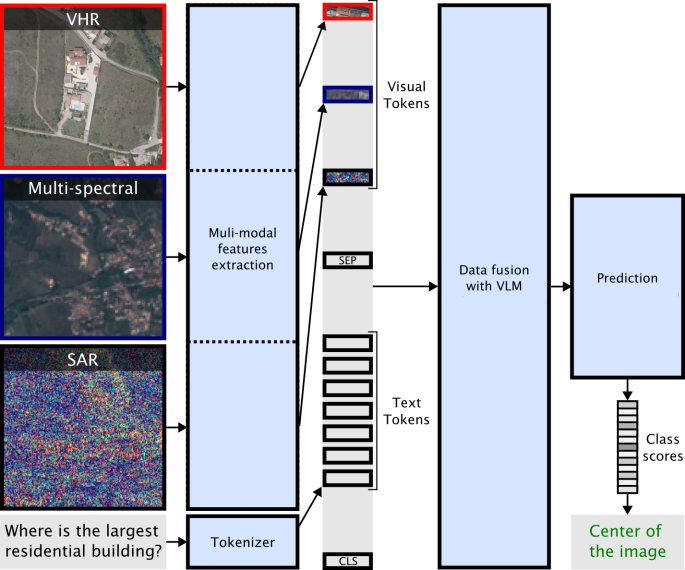
\includegraphics[width=\columnwidth]{images/TAMMI/architecture.png}
    \caption{Graphical outline of the proposed MM-RSVQA (\textit{Multi-modal Multi-resolution} RSVQA) architecture.
    The inputs of the model (multi-modal imagery and textual question) are represented on the left and the output (predicted answer) is on the bottom right. First, we extract features from each image modality and perform a text embedding. These features are passed through a vision-language model (VLM) to obtain a vector which can be classified among a set of pre-defined answers.
    The different blocks composing the system are detailed in \autoref{sec:method}.}
    \label{fig:method}
\end{figure}


\subsection{Transformer-based data fusion}
\label{ssec:fusion}
We first project the visual features obtained through the feature extractor to a 768-dimensional vector through a linear layer. The 768-dimensional visual feature is concatenated with a [SEP] token, which marks the separation between visual and textual tokens, and then with the textual embeddings. Finally, a [cls] token is added to  represent the entire input.%, making the fusion step more sophisticated than the traditional point-wise multiplication used previously in the literature \cite{lobry2020rsvqa,lobry2021rsvqa}.
%\textcolor{red}{What is also important is to say that we are not going to do a classic fusion (pointwise multiplication) but that we are going to do it in a system able to exploit the complementarity of multi-modal information, depending on the question in an end-to-end manner.}

To process the diverse features, we leverage VisualBERT~\cite{li2019visualbert}, a state-of-the-art vision-language model designed for the integration of visual and textual features. 
VisualBERT uses a stack of transformer layers to align regions in the images with the text input through self-attention mechanisms. 
Pre-trained on image-caption pairs, VisualBERT uses objectives as image-text matching and masked language modeling. It is effective for various tasks, such as VQA, visual commonsense reasoning, natural language for visual reasoning, and region-to-phrase grounding.

The cornerstone of the proposed method is therefore to learn jointly and in an end-to-end manner an optimized representation of the data and a fusion process. 
The latter makes it possible to exploit the complementarity of multi-modal information and to weight the best modalities, according to the visual content of the scene studied, the types of questions, and the expected answers.


\subsection{Prediction}
\label{ssec:pred}
The data fusion part of our architecture outputs a 768-dimensional vector that represents the fused multi-modal features. In this model, we frame the VQA as a classification task. Therefore, this vector is passed through a linear layer that maps it to a $k$-dimensional output.


\begin{table*}[!t]
\centering
\footnotesize
\begin{tabular}{llcccccc}
\cline{4-8}
& & & \multicolumn{4}{c}{\textbf{Ablation studies}} \\
\hline
\textbf{Category} & \textbf{Question Type} & \textbf{MM-RSVQA} & \textbf{VHR} & \textbf{MS RGB + VHR} & \textbf{MS + VHR} & \textbf{SAR + VHR} & \textbf{MS + SAR}\\
\hline
\multirow{3}{*}{\textbf{Presence Questions}} 
    & Presence & \ 96.87 & 95.41 & 96.58 & 96.79 & \textbf{97.00} & 96.84 \\
    & Flood Presence & 98.04 & 94.02 & 97.78 & 97.84 & 96.85 & \textbf{98.11} \\
    & Mountain Presence & \textbf{98.80} & 95.76 & 98.75 & 98.49 & 97.75 & 98.59 \\
\hline
\multirow{4}{*}{\textbf{Quantity Questions}} 
    & Count & \textbf{51.76} & 49.73 & 50.99 & 50.89 & 50.59 & 51.22\\
    & Density & \textbf{26.46} & 26.17 & 26.40 & 26.45 & 26.42 & 26.44 \\
    & Area & 10.28 & 10.28 & 10.30 & 10.12 & \textbf{10.33} & 10.32  \\
    & Percentage & \textbf{41.66} & 41.58 & \textbf{41.66} & 41.60 & \textbf{41.66} & 41.62 \\
\hline
\textbf{Location Questions} 
& Absolute Location & 17.17 & 17.15 & \textbf{17.21} & 16.89 & 17.04 & 17.18\\
\hline
\multirow{9}{*}{\textbf{Classification Questions}} 
    & Water & \textbf{89.38} & 81.10 & 87.73 & 88.65 & 83.14 & 88.23 \\
    & Vegetation & \textbf{53.06} & 48.57 & 50.92 & 51.00 & 48.57 & 50.83 \\
    & Flood Level & \textbf{80.92} & 75.68 & 79.19 & 79.27 & 75.68 & 79.54 \\
    & Flood Type & \textbf{97.91} & 90.60 & 95.68 & 96.93 & 95.54 & 97.32 \\
    & Land Cover & 74.76 & 68.79 & 72.53 & 72.42 & \textbf{74.89} & 74.27 \\
    & Urban & \textbf{93.78} & 69.20 & 90.33 & 91.58 & 92.40 & 93.32 \\
    & Department & \textbf{98.96} & 89.78 & 97.39 & 97.58 & 98.03 & 98.47 \\
    & Region & 99.98 & 99.96 & \textbf{99.99} & 99.92 & \textbf{99.99} & \textbf{99.99} \\
    & Mountain Name & 99.89 & 99.94 & \textbf{99.96} & 99.91 & 99.89 & \textbf{99.96} \\
\hline
\multirow{4}{*}{\textbf{Relation Questions}} 
    & Distance & \textbf{9.08} & \textbf{9.08} & 9.07 & 9.07 & 9.05 & \textbf{9.08} \\
    & Comparison & \textbf{98.43} & 98.25 & 98.34 & 98.36 & \textbf{98.43} & 98.41 \\
    & Relative Location & 17.99 & 18.10 & 17.77 & 17.62 & \textbf{18.17} & 17.74 \\
    & Nearest & 21.57 & \textbf{21.71} & 20.56 & 20.89 & 20.96 & 20.74\\
    
\hline
& \textbf{Average Accuracy} & \textbf{65.56} & 61.94 & 64.72 & 64.87 & 64.40 & 65.15 \\
& \textbf{Overall Accuracy} & \textbf{55.11} & 52.22 & 54.41 & 54.49 & 54.29 & 54.70 \\
\cline{2-8}
\end{tabular}

\caption{Accuracy for the VQA task on the TAMMI dataset.
Comparison of MM-RSVQA, VHR, MS RGB + VHR, MS + VHR, SAR + VHR, and MS + SAR across question types. Highest scores (per question type) are shown in bold.}

%\TODO{double check before to submit that the bold scores are the best}}
\label{tab:results}

\end{table*}



\section{Results and discussion}
\label{sec:results}

We present preliminary performances of the proposed method MM-RSVQA on the TAMMI dataset. With respect to the RSVQA task, we discuss the contribution (and complementarity) of the different imaging modalities with regard to the different types of questions (and answers) constituting the dataset.

\subsection{Experimental settings}
\paragraph{Dataset splitting}
The dataset is randomly split into training, validation, and test sets based on the images with a proportion of 60\%, 20\%, and 20\% respectively. We use the validation set for the tuning of the hyper-parameters described in the rest of this section. For the training, we consider only the questions having an answer in the top $k=1'000$ most frequent answers.This parameter is fixed for dimensionality reduction, as done in ~\cite{antol2015vqa}, ~\cite{lobry2020rsvqa}, covering 86.6\% of train answers. While we consider all the samples of the test set.
\paragraph{Full pipeline}
We use a frozen ResNet-152 model pre-trained on ImageNet for the orthophotos feature extractor and two ResNet-50 models pre-trained on BigEarthNet~\cite{sumbul2021bigearthnet} for the MS and SAR feature extractors. 
We set $\lms = $ 100 and $\lsar = $ 200. 
We use a cross-entropy loss, optimized with Adam. For the training of MM-RSVQA, we set the learning rate to $3\times 10^{-5}$, the batch size to 80 samples and the number of epochs to five.

\subsection{Metrics}
Three metrics are used to evaluate the VQA results: the per-class accuracy, overall accuracy (OA) and average accuracy (AA). 
The per-class accuracy is defined as the ratio of correct answer with the total number of questions for one of the 21 question types. 
The overall accuracy is the ratio of correct answers with the total number of questions in the dataset. 
Finally, the average accuracy is the arithmetic mean of the per-class accuracies.

\subsection{Quantitative results}
To evaluate the proposed architecture and the TAMMI dataset, we conduct experiments using our main model MM-RSVQA and we perform ablation studies with various combinations of modalities. 
The results are presented in Table \ref{tab:results}. We show the performances of the MM-RSVQA model (using VHR, MS and SAR modalities) and ablation studies across question types, highlighting the contributions of each modality in the context of this challenging task.

\paragraph{MM-RSVQA} 
The proposed multi-modal multi-resolution baseline model, as seen in Table \ref{tab:results}, achieves strong performance across most question types and outperforms models using only one or two modalities. This highlights the advantage of integrating multiple modalities for the RSVQA task. 
Notably, MM-RSVQA demonstrates high accuracy through categories such as presence, comparison, water and region. 
These results indicate that combining VHR, MS, and SAR data helps the model to better identify objects, to assess quantities, and to improve classification accuracy. 
For some question types, such as absolute location, area and relative location, the model shows lower accuracy. This suggests that these questions types are more challenging due to the difficulty of understanding spatial relationships or precisely locating objects. One hypothesis is that the added trainable parameters when adding MS and SAR modalities requires more training samples than for other models. %\TODO{CHECK BEFORE SUBMITTING} 

\paragraph{Ablation study} 
To evaluate the contribution of the different modalities we perform ablations studies at the input level. The results, shown in Table \ref{tab:results} present the accuracy of different configurations: VHR only; MS RGB + VHR (only keeping the RGB bands of Sentinel-2 and VHR patch); MS + VHR (10 bands of Sentinel-2 and VHR patch); SAR + VHR; and MS + SAR (Sentinel-1 SAR images + 10 bands of Sentinel-2).

From these results we observe that using VHR only does not allow to obtain good results. Despite the fact that the questions only concern the geographical extent of the VHR patch, it appears that providing additional context, either through MS or SAR, brings better performances. This is clearly visible in classification questions such as department or urban. This suggests that the integration of SAR and multi-spectral data enhances the ability of the model to understand and classify complex features. This validate the main hypothesis of this work: additional context, even if the question is restricted to a set geographical extent, improve performances.

By comparing MS RGB + VHR and MS + VHR, we can see that the performances are similar, with a small improvement for the model considering the 10 spectral bands of Sentinel-2 despite the added parameters. This validate the approach taken in other datasets considering Sentinel-2 data (RSVQA LR, RSVQAxBEN, see \autoref{tab:Overview}) which only considered the RGB channels. However, to the best of our knowledge, it is the first time that this hypothesis is experimentally demonstrated for VQA.

Regarding the SAR modality, we can see that SAR + VHR obtains similar performances to MS + VHR. This indicates that the benefits of adding context holds whether the modality. However, it appears that SAR is particularly efficient at discriminating certain features, such as land cover. Finally, our experiment with MS + SAR modalities indicates that jointly considering both modalities is a strong advantage for the model. Indeed, despite not having the very high resolution data, this model obtains the second best overall performances behind MM-RSVQA.

%On the other hand, by comparing VHR and MS RGB + VHR, we can see that adding broader context, such as a larger geographical area (covered by the MS patch), enhances the accuracy of the model. 
%This is best displayed by questions categories such as Urban (increase of 20\%) and Departement (increase of 7\%). For the MS + VHR configuration, we observe that adding extended multi-spectral information generally helps improve accuracy compared to VHR and MS RGB + VHR, especially classification questions. We can therefore conclude that richer spectral information helps distinguish finer environmental features. Finally, for SAR + VHR configuration we observe that adding SAR improves the accuracy of certain questions types such as Land Cover, Area and Presence, suggesting the model benefits from SAR's ability to capture surface texture and structure. 
%\begin{table*}[h]
%\centering
%\footnotesize
%\begin{tabular}{|l|l|l|l|l|l|c|c|c|c|c|c|c|c|c|c|c|} \hline 

%\multirow{2}{*}{\textbf{Model}}  & \multicolumn{3}{|c|}{Used modalities} &\multicolumn{2}{|c|}{Model param.}&     \multicolumn{9}{|c|}{Per-question accuracy}&\multicolumn{2}{|c|}{Dataset metrics}\\ \cline{2-17}  
%  & Ortho& MS&SAR & Att.&Seg.&     1.(a)& 1.(b)& 1.(c)&1.(d)& 2.(a)& 3.(a)&4.(a)& 4.(b)&4.(c)&AA&OA\\ \hline \hline

%Proposed& \checkmark& \checkmark& \checkmark& \checkmark&\checkmark&     & & && & && &&44.41 & 42.21    \\ \hline\hline
%A1& \checkmark& & & \checkmark&\checkmark& 91.57     &25.64 &63.43 &29.38&  14.58 &95.44&14.58 &20.10& 74.19 &45.42 &  47.74 \\ \hline  

%A2& \checkmark& \checkmark& & \checkmark&\checkmark&84.36 & 17.12 & 42.40 & 22.26 & 13.29 & 75.39 & 11.48 & 12.71 & 55.83 & 36.48 & 37.20 \\ \hline  

%A3& \checkmark& & \checkmark& \checkmark&\checkmark& 88.99& 23.89& 56.98 & 26.51 & 14.90 & 92.52 & 12.40 & 15.48 & 73.70 & 42.83 & 45.04 \\ \hline\hline  

%M1  & \checkmark &\checkmark & \checkmark & \checkmark&  & 78.21& 06.30&  26.11& 14.40 &13.13 & 72.35&13.62 & 11.61& 31.76&31.76 & 29.73  \\ \hline 

%M2  & \checkmark & \checkmark & \checkmark & && 79.11 &09.34& 36.62    & 18.99&12.40 &71.68&12.33 &12.40 &36.97&33.07 & 32.21 \\ \hline  



%\end{tabular}
%\caption{Results of our proposed model and ablation studies. All of the results are accuracy percentages.}
%\label{tab:res}
%\end{table*}


\section{Conclusion and limitations}
In this work, we address the VQA on Remote Sensing data problem by utilizing multi-modal and multi-resolution data. With these diverse modalities, we show that a model can benefit from their complementarity, in terms of coverage, spectral resolution, spatial resolution and physical information. 
This represents a new challenge for the vision community, as the interaction between different image modalities, beyond RGB, and text remains under-explored.  To support this new problem, we propose a new dataset, named TAMMI, which contains 21 types of questions based on very high resolution patches (orthophotos), high-resolution multispectral data (Sentinel-2), and Synthetic Aperture Radar (Sentinel-1) images. The dataset spans three French departments, each with distinct landscapes, allowing for diverse and challenging questions. 

%We introduce a baseline model to process the multi-modal images and the textual input data based on the VisualBERT architecture. Our results indicate that multi-resolution and multi-modal data enhance the model performances. The VHR modality is useful for tasks requiring high-detail images. For tasks requiring a broader context, the contributions from the SAR and MS modalities proves to be substantial. In our pipeline, we use all three modalities together, but the approach can be easily adapted to use only one or two modalities depending on availability. On the other hand, we show that using very high resolution RGB images alone does not allow, in our setting, to obtain good performances.
We introduce a baseline model to process multi-modal images and textual input data based on the VisualBERT architecture. Our results indicate that multi-resolution and multi-modal data enhance model performance. The VHR modality is useful for tasks requiring high-detail images. For tasks requiring a broader context, the contributions from the SAR and MS modalities prove to be substantial. In our pipeline, we use all three modalities together. However, ablation studies show that even when one modality is missing, the proposed model obtains better performances compared to VHR RGB orthophotos alone. This is a strong result, as this modality is the one commonly used in RSVQA.

%Future work is required to improve the modeling on this dataset. Indeed, dedicated feature extractors, leveraging the continuous spectral information of the MS modality or the physical information of SAR could be beneficial. By releasing this dataset, we provide a new challenging task. Thanks to the dynamic context selection for the MS and SAR patches, this dataset can be also used for a wide range of additional multi-modal tasks, besides VQA. Additionally, the provided dataset can easily be extended to include more regions, further enhancing its generalization and performance across diverse landscapes and environments.

Future work includes developing better models using specialized feature extractors for multispectral and SAR data. This dataset introduces a challenging task and, thanks to dynamic context selection, supports a variety of multi-modal applications beyond VQA. It is also easily extensible to cover more regions, promoting better generalization across diverse landscapes and environments.


\clearpage
%\setcounter{page}{1}
%\maketitlesupplementary
%\setcounter{section}{1}

\section*{SAR data (Sentinel-1) pre-processing}
The pre-processing pipeline to generate continuous SAR (Sentinel-1) patches consists of several steps including SAR and VHR data. 
We describe hereinafter each step in details:
\begin{enumerate}
    \item We use the algorithm presented in~\cite{weissgerber2022labsar} to find the position of the center of the VHR patch in the SAR image. To do so, we need the geographical position of the center of the VHR patch. This position must include altitude, due the geometrical distortions inherent in SAR, particularly layover;
    
    \item The latitude and longitude of the VHR patches are extracted from the meta-data of the image. Using this latitude and longitude, the altitude is given by this \href{https://geoservices.ign.fr/documentation/services/services-deprecies/calcul-altimetrique-rest}{https://geoservices.ign.fr/documentation/services/services-deprecies/calcul-altimetrique-rest} and these information are stored in a JSON file, \textit{latlonalt.json};
    
    \item The Sentinel-1 Single Look Complex (SLC) images are separated in three swath. To find the correct swath, the projection of the geographical point is applied, using the meta-data linked to each swath. The only swath for which the algorithm returns a valid position is selected;
    
    \item In each swath, the S1 image is divided in different overlapping bursts, that are all stored in the same file separated by black lines. 
    The S1 images need to be debursted (removing of the black line and of the overlap) to get a continuous image before to extract the S1 patch that is inputted in the model. 
    This debursting is done using meta-data of the S1 image and by comparing the two consecutive burst. A result of the debursting process is shown in Figure \ref{fig:sarprepostdeburst}.
    The debursted images are provided with the dataset. The projection algorithm is thus modified to give the position in this new deburst file. This position and the correct swath are stored in the JSON file containing all information on the VHR patches;
    
    \item When a patch of size $\lsar$ $\times$ $\lsar$ ($\lsar$ specified by the user) is extracted, the two polarimetric channels are converted in dB, and the ratio is computed. A tail-value elimination procedure is performed on each channel separately using statistics information extracted over the whole dataset.
\end{enumerate}
 %   \footnotetext{https://geoservices.ign.fr/documentation/services/services-deprecies/calcul-altimetrique-rest}


\begin{figure}[!ht]
    \centering
    \begin{subfigure}[b]{0.49\columnwidth}
        \centering
        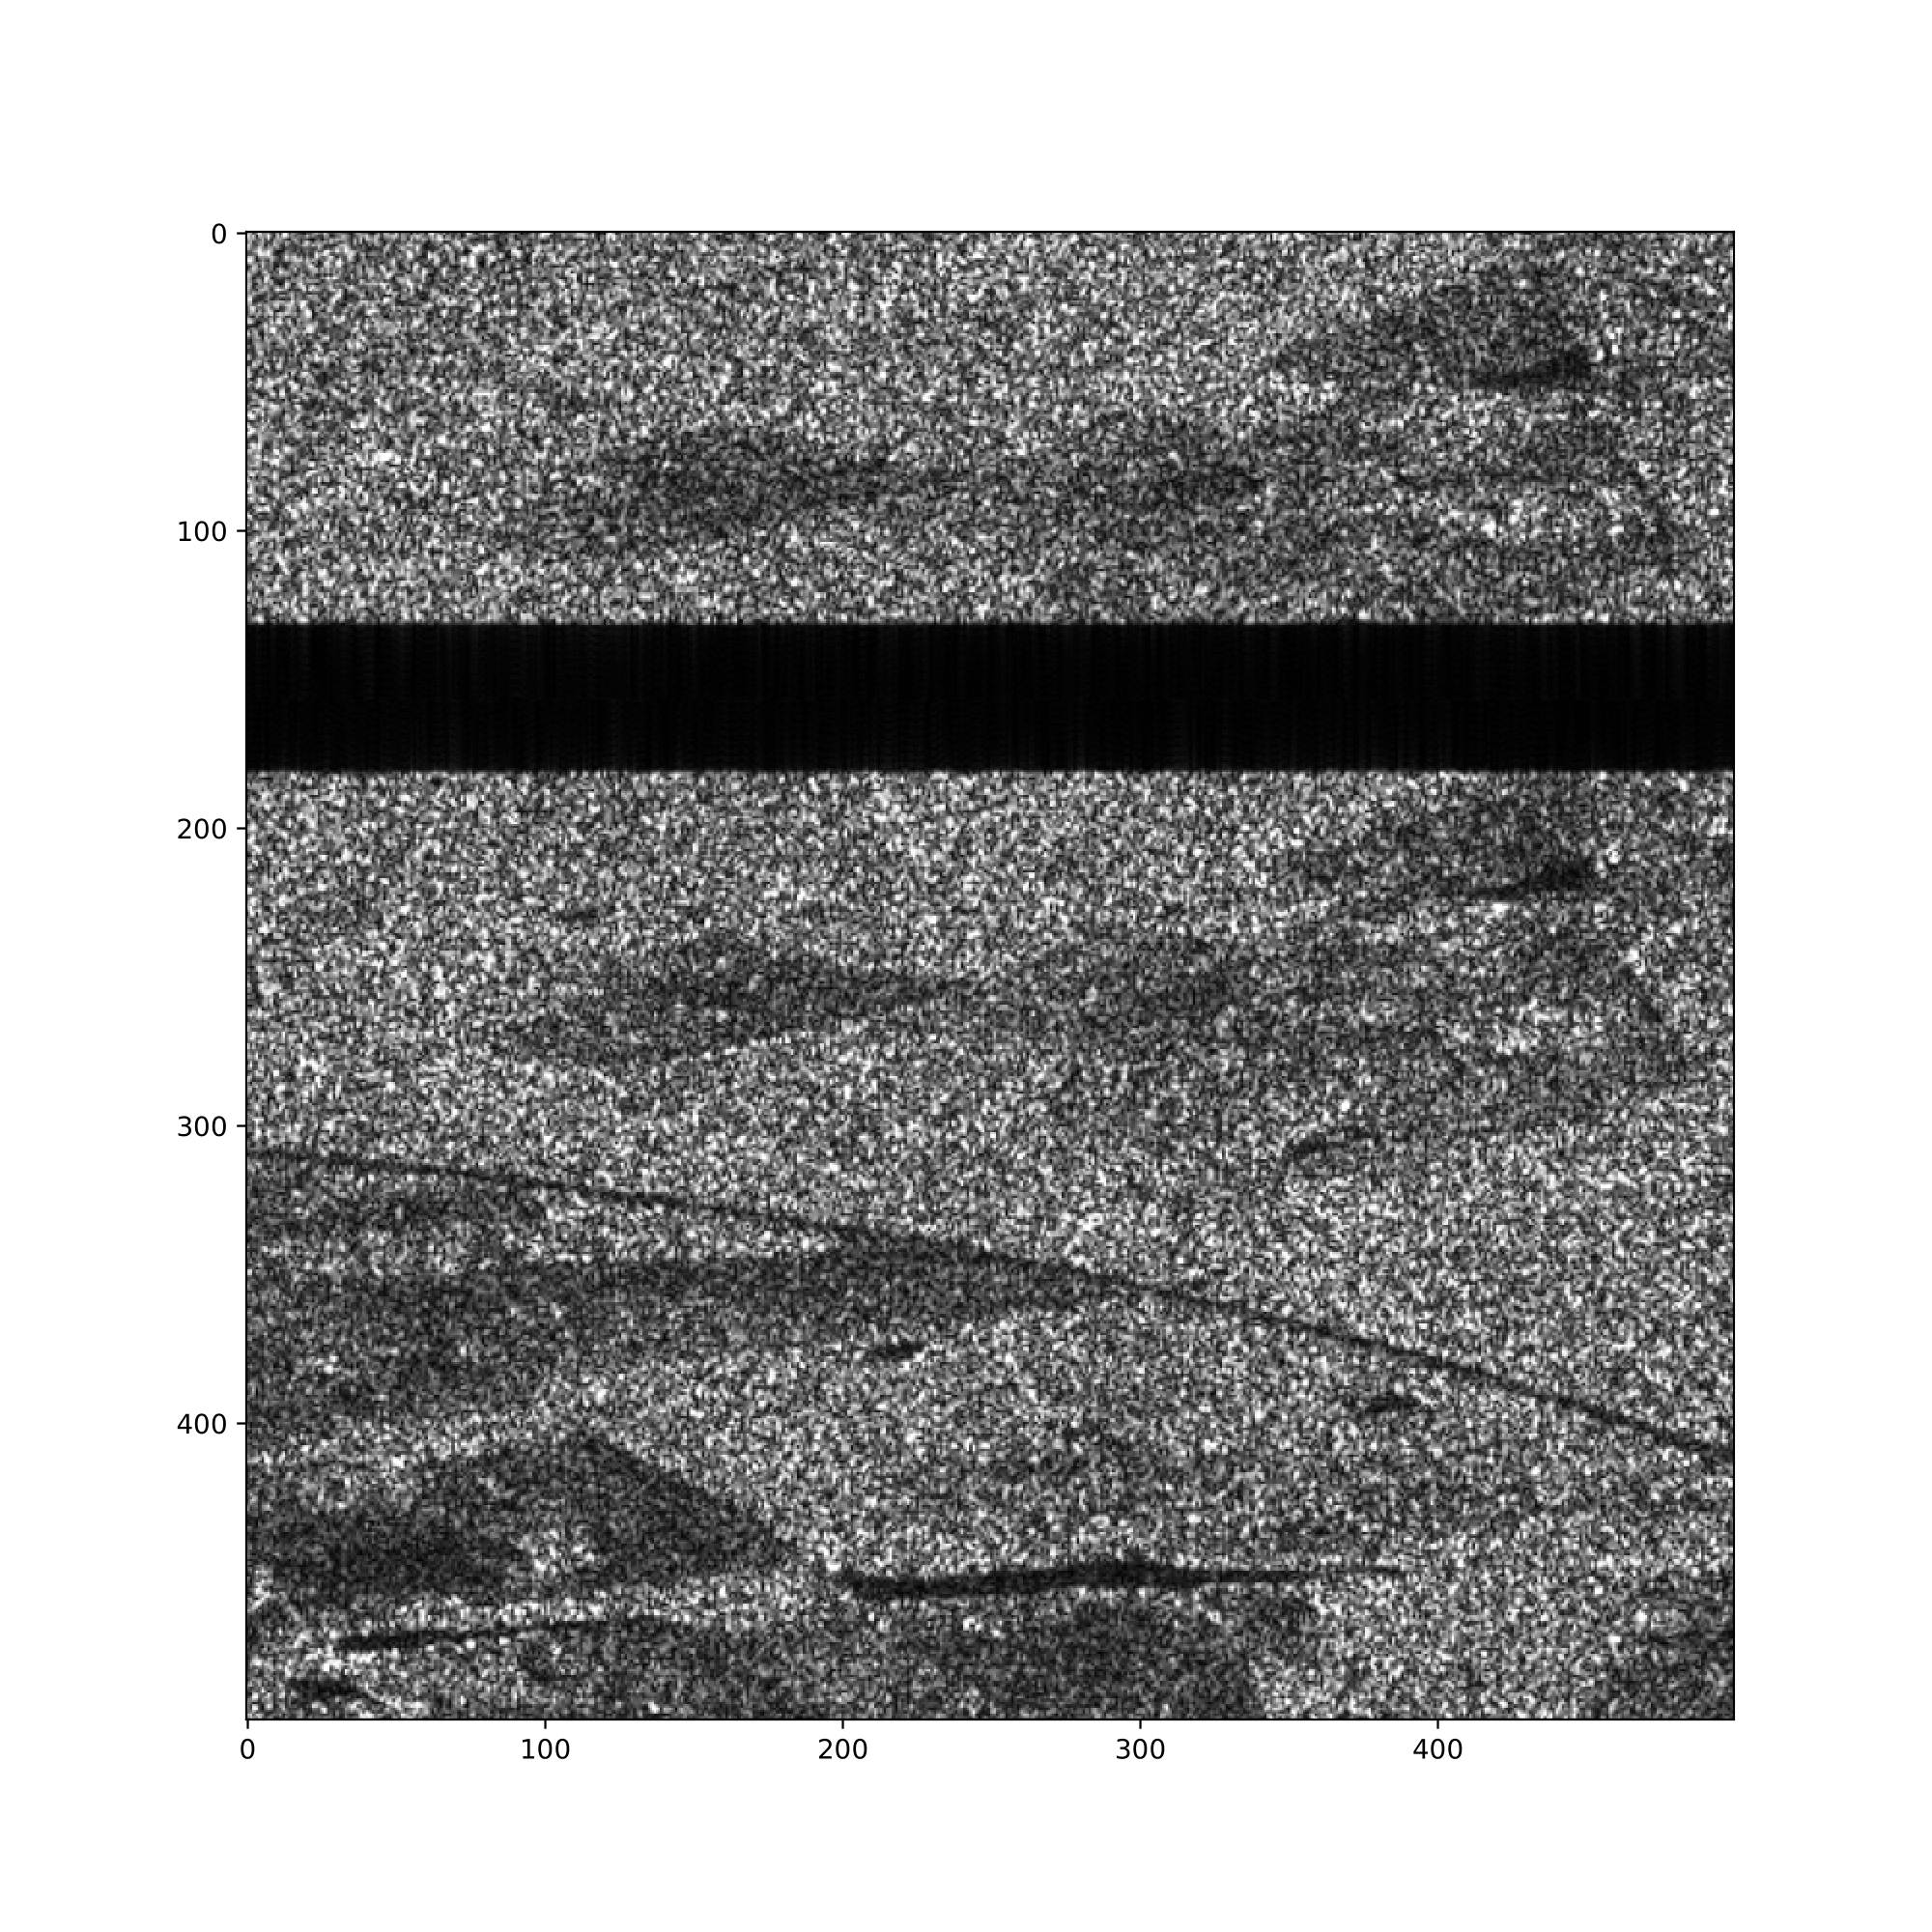
\includegraphics[width=\textwidth,trim={1.5cm 1.5cm 1.5cm 1.5cm},clip]{images/TAMMI/original_patch.png}
        \caption{Pre-debursting}
        \label{fig:sub1}
    \end{subfigure}
    \begin{subfigure}[b]{0.49\columnwidth}
        \centering
        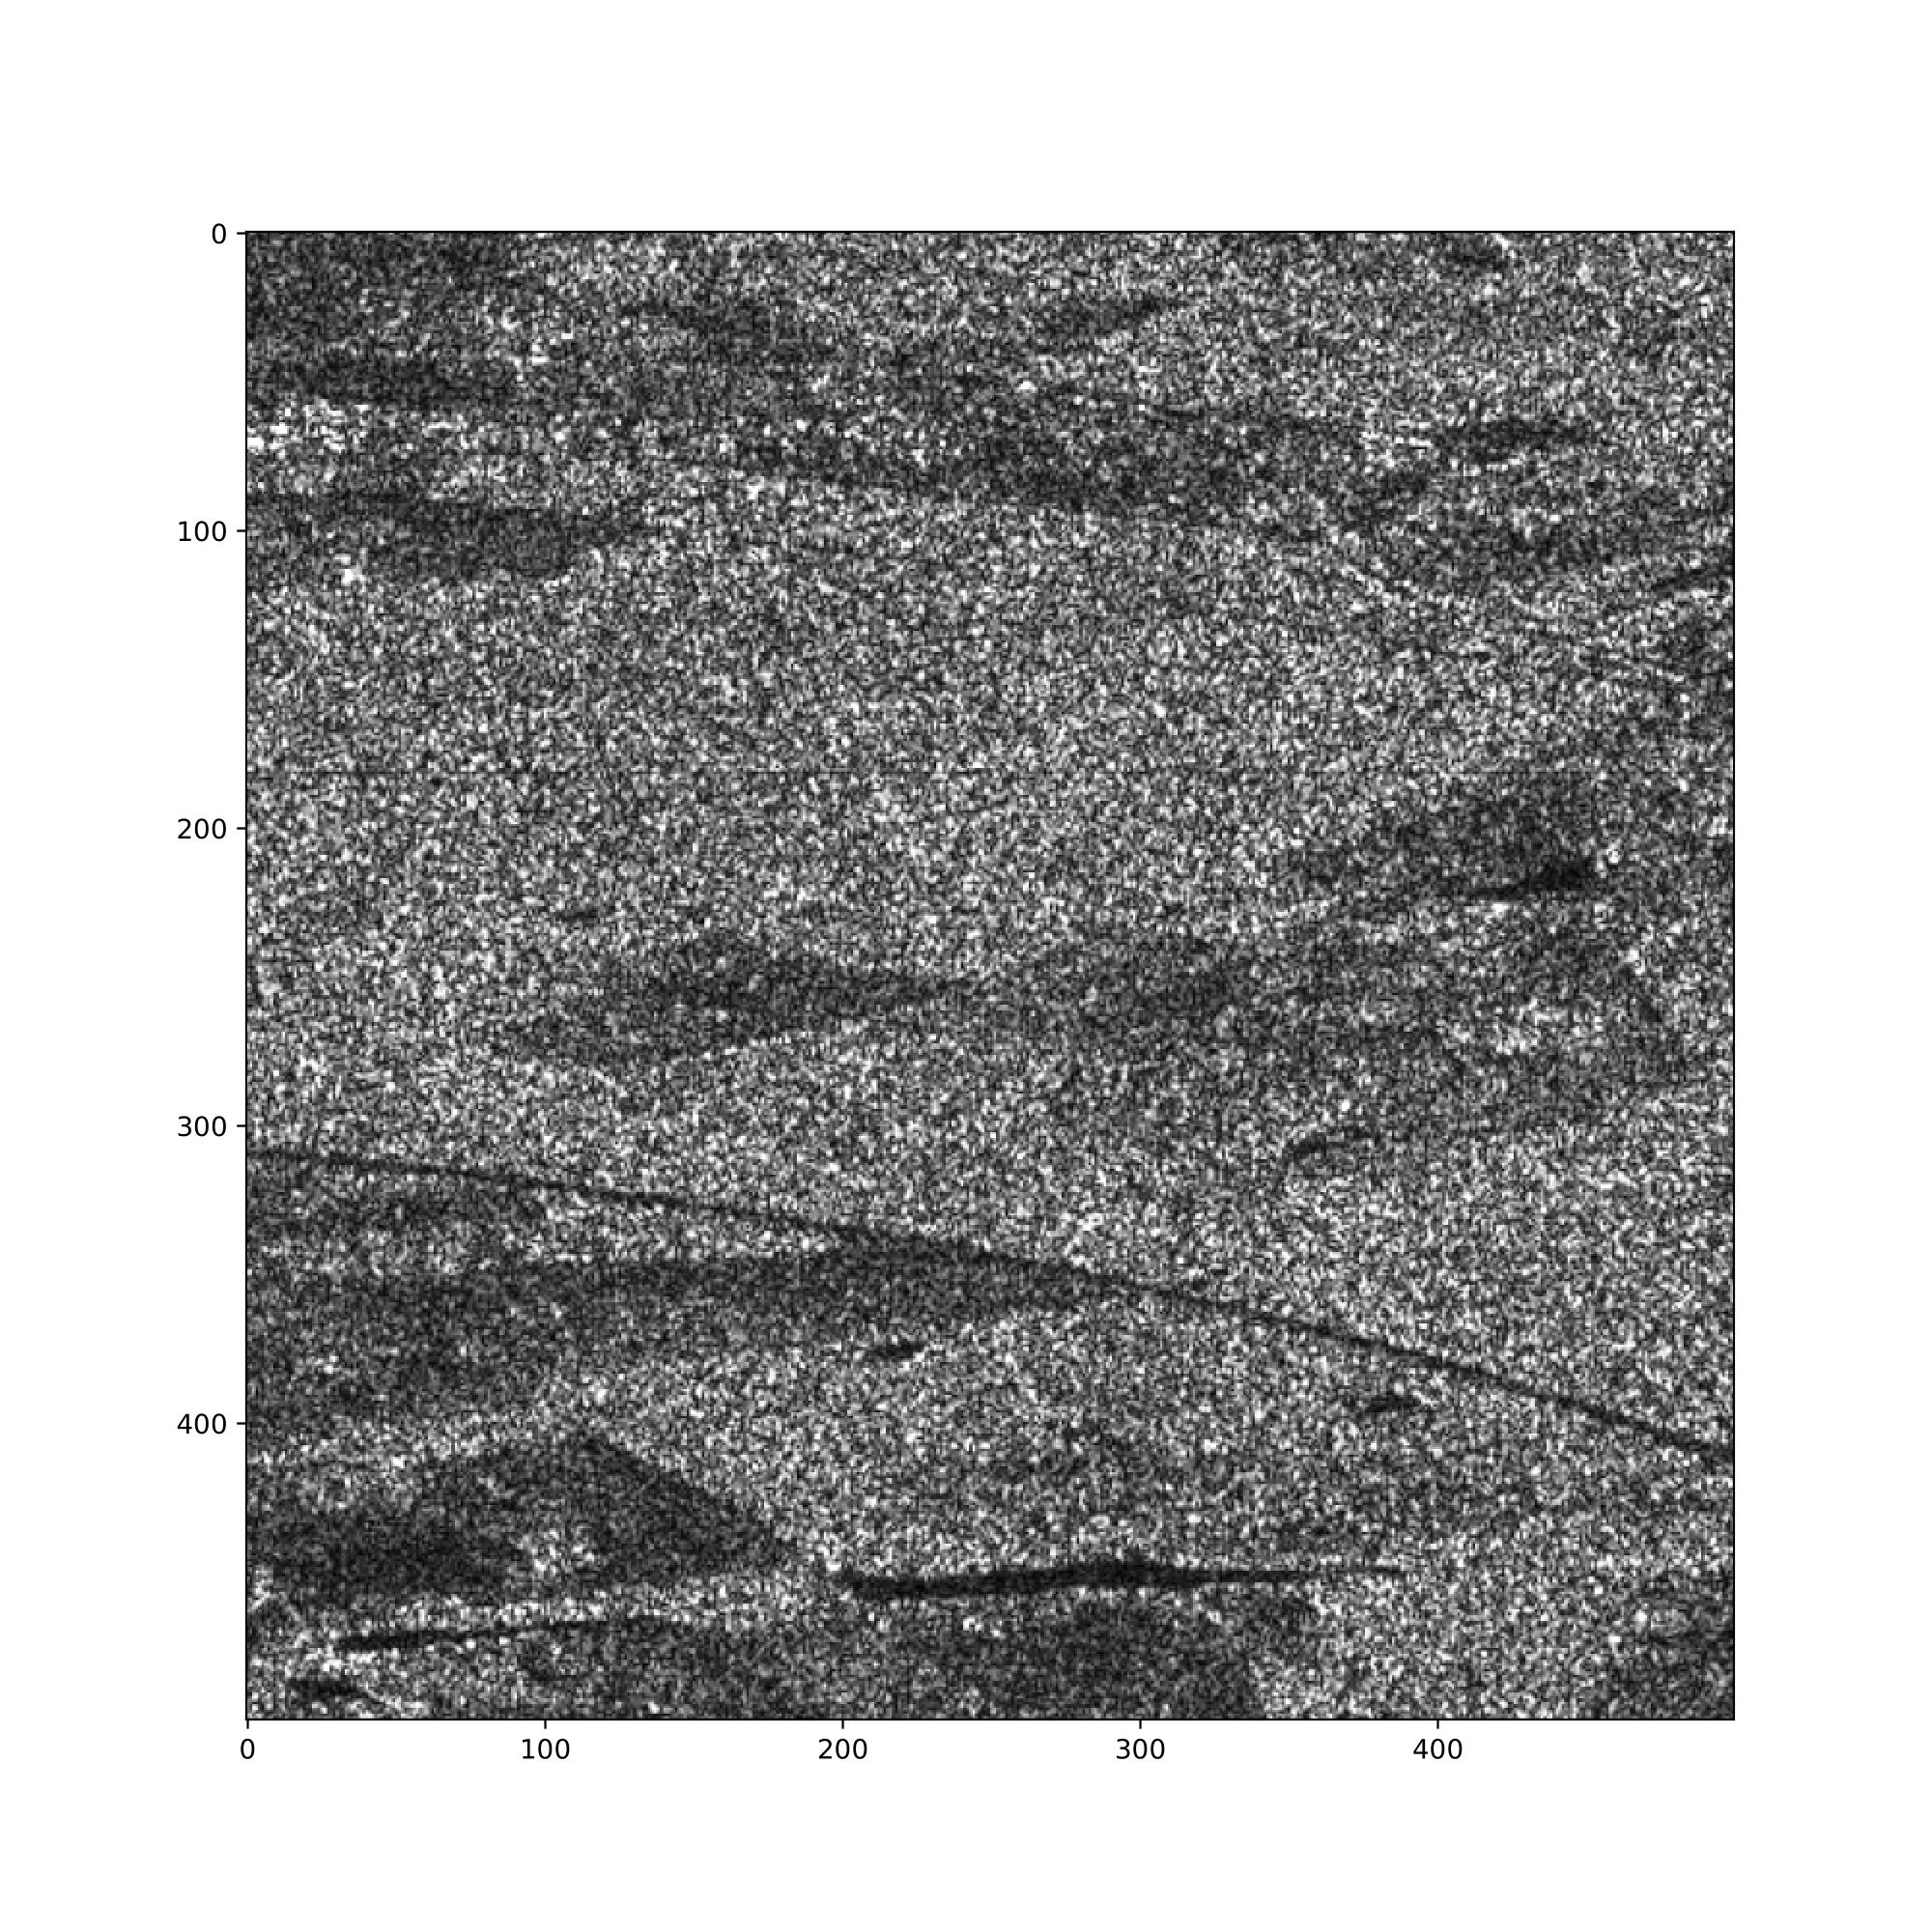
\includegraphics[width=\textwidth,trim={1.5cm 1.5cm 1.5cm 1.5cm},clip]{images/TAMMI/final_patch.png}
        \caption{Post-debursting}
        \label{fig:sub2}
    \end{subfigure}
    \caption{Sentinel-1 SLC images before (a) and after (b) the application of the proposed debursting method. 
    The visualization is done using a threshold of 233.}
    \label{fig:sarprepostdeburst}
\end{figure}

\newpage
\clearpage



%\part{Toward Multi-Task Synergies}
%% ============================================================
% CHAPTER: Multi-Task Study -- Reconstruction, Captioning, and VQA
% Adapted from the QUEST conference submission draft.
% Follows the conventions established in Chapters 3-5:
% chapter summary inside \printmyminitoc, section-level intro
% paragraphs, an explicit Positioning subsection in Related Work.
% ============================================================
\titlespacing*{\chapter}{0pt}{-35pt}{40pt}
\chapter{A Multi-Task Study of Reconstruction, Captioning, and VQA}
\label{chap:multitask}
\startcontents[chapters]
\printmyminitoc{
\textit{Chapter summary.} The preceding chapters treated visual question answering as the sole training objective,
 whether on a single modality (Chapters~\ref{chap:llm_augmentation} and~\ref{chap:seg_attention}) or on the three co-registered modalities of TAMMI 
 (Chapter~\ref{chap:tammi}). This chapter instead studies what happens when RSVQA is trained jointly with captioning 
 and self-supervised image reconstruction, extending TAMMI with LLM-generated captions to support this joint setting. 
 This chapter compares four training configurations, full multi-task training, multi-task 
 training without reconstruction, VQA-only, and captioning-only, to measure the specific contribution of each additional 
 objective rather than the combination as a whole.
}
% ============================================================
\section{Introduction}
\label{sec:chap6_intro}

The previous two chapters extended RSVQA along two axes independently:
attention design (Chapter~\ref{chap:seg_attention}) and modality/resolution
coverage (Chapter~\ref{chap:tammi}). Both chapters, however, treated
RSVQA as the only training signal. Section~\ref{sec:rw-captioning-challenges}
already noted, in reviewing the RS literature, that models
combining RSVQA with other tasks (captioning in particular) are
increasingly common, but that the benefit of doing so is rarely measured
directly, and that where it has been measured, results are mixed rather
than confirmatory: RS-LLaVA's own reported results show single-task
fine-tuning outperforming joint training on both captioning and VQA
metrics, directly contradicting the premise behind combining the two
tasks. This chapter takes that open question as its object of study.

Remote sensing imagery is open to more than one training signal
beyond question answering. Captioning provides a free-form description
of a scene that is not constrained to a fixed answer vocabulary, and
self-supervised reconstruction provides a training signal that requires
no annotation at all, only the imagery itself. In principle, jointly
optimizing these three objectives, reconstruction, captioning, and VQA,
could encourage a shared representation that is more robust than any
one objective alone: reconstruction could preserve visual detail that a
purely discriminative VQA loss might discard, and captioning could
provide a richer, less templated supervisory signal than RSVQA's
templated question-answer pairs. Whether this potential is realized in
practice is what this
chapter investigates.

This chapter makes three contributions. First, we extend the TAMMI
dataset (Chapter~\ref{chap:tammi}) with LLM-generated captions,
producing a new RS benchmark supporting
reconstruction, captioning, and VQA jointly across the same
optical/multispectral/SAR triplets. Second, we introduce QUEST
(Questioning and Understanding Earth Observation Images
through Text), a unified
architecture that jointly optimizes global cross-modal contrastive
alignment, patch-level cross-modal alignment, per-modality
reconstruction, and a shared generative decoder for captioning and VQA,
so that all four objectives can be selectively enabled or disabled
within a single model rather than requiring separate architectures per
configuration. Third, rather than reporting a single best configuration,
we conduct a controlled study comparing four training configurations,
full multi-task training, multi-task training without reconstruction,
VQA-only, and captioning-only, isolating the contribution of
reconstruction and of joint training itself, respectively.

The remainder of this chapter is organized as follows.
Section~\ref{sec:chap6_related} reviews related work on multi-modal RS
datasets, RS vision-language models, self-supervised multi-modal RS
representation learning, and unified generative frameworks, and
positions this chapter's ablation-based study relative to each.
Section~\ref{sec:chap6_dataset} describes the caption extension of
TAMMI. Section~\ref{sec:chap6_method} presents the architecture and
training objectives. Section~\ref{sec:chap6_experiments} reports and
discusses the results of the four-configuration study.
Section~\ref{sec:chap6_conclusion} concludes and discusses limitations.

\section{Related Work}
\label{sec:chap6_related}

This section reviews four bodies of work relevant to this chapter's
study. Section~\ref{sec:chap6_rw_datasets} reviews multi-modal RS
datasets.
Section~\ref{sec:chap6_rw_vlm} reviews RS vision-language models that, combine multiple language-producing tasks, but
without isolating each task's contribution. Section~\ref{sec:chap6_rw_ssl}
reviews self-supervised multi-modal RS representation learning, which
grounds cross-modal alignment without language. Section~\ref{sec:chap6_rw_unified}
reviews unified generative frameworks outside RS. Section~\ref{sec:chap6_positioning}
then positions this chapter's contribution relative to all four.

\subsection{Multi-Modal Remote Sensing Datasets}
\label{sec:chap6_rw_datasets}

The availability of large-scale, annotated multi-modal datasets has
been a key driver of progress in Earth observation.
\textcite{schmitt2019sen12mscurateddataset} established an early benchmark with
SEN12MS, providing 180,662 co-registered Sentinel-1 SAR and Sentinel-2
multispectral image triplets paired with MODIS land cover maps, enabling
data fusion research at scale. \textcite{sumbul2019bigearthnet} extended
this effort with BigEarthNet, 590,326 Sentinel-2 patches annotated with
multi-label CORINE land cover classes, later expanded to include paired
Sentinel-1 imagery. More recently, BigEarthNet.txt~\cite{herzog2026bigearthnettxt}
enriched the BigEarthNet corpus with around 9.6 million text
annotations, including geographically anchored captions, VQA pairs, and
referring expression instructions over co-registered Sentinel-1/2
pairs, and ChatEarthNet~\cite{yuan2024chatearth} provides 163K
Sentinel-2 image-caption pairs generated using a general-purpose LLM,
covering global land cover types. Despite this progress, none of these
datasets incorporate VHR RGB imagery alongside SAR and multispectral
data at the resolution TAMMI does; conversely, TAMMI itself
(Chapter~\ref{chap:tammi}) supports VQA but not free-form captioning.
%This chapter extends TAMMI with LLM-generated captions to close that
%gap, discussed in full in Section~\ref{sec:chap6_dataset}.

\subsection{Vision-Language Models for Remote Sensing}
\label{sec:chap6_rw_vlm}

Early vision-language work in RS focused on adapting contrastive
image-text pretraining to the domain. RemoteCLIP~\cite{liu2024remoteclip}
was the first vision-language foundation model tailored to RS, training
a CLIP-style model on a scaled dataset built by converting heterogeneous
annotations into image-caption pairs. RS-M-CLIP~\cite{silva2024rsmclip}
extended this to multilingual settings, showing that aligning local and
global representations improves cross-modal retrieval. These contrastive
models are effective for retrieval and zero-shot classification but do
not support generative tasks such as captioning or VQA.

Instruction-tuned VLMs have since expanded the scope of language-driven
RS analysis. GeoChat~\cite{kuckreja2024geochat} was the first grounded
VLM for RS, fine-tuning LLaVA-1.5 on a curated RS instruction dataset to
support image and region captioning, VQA, scene classification, and
referring object detection on high-resolution RGB imagery. EarthDial~\cite{soni2025earthdialturningmultisensoryearth}
scales this paradigm further, fine-tuning InternVL on an
instruction dataset spanning RGB, multispectral, SAR, and multi-temporal
data, and SkyEyeGPT~\cite{zhan2025skyeyegpt} similarly unifies multiple
RS vision-language tasks via instruction tuning. All of these approaches
adapt a pretrained LLM through projection layers without explicitly
enforcing cross-modal spatial alignment: the model has no mechanism to
associate co-registered patches from different sensors in the embedding
space beyond what is implicitly learned through language supervision.
%None of these works
%isolates the contribution of the individual tasks their instruction
%data combines.

\subsection{Multi-Modal Representation Learning in Earth Observation}
\label{sec:chap6_rw_ssl}

A parallel line of work learns grounded multi-modal representations
through self-supervised objectives, without language.
DINO-MM~\cite{scheibenreif2022dinomm} applies a DINO-style
self-supervised framework jointly to Sentinel-1 and Sentinel-2 pairs,
learning complementary SAR-optical representations via intra- and
inter-modality objectives. CROMA~\cite{fuller2023croma} combines
cross-modal contrastive learning with masked autoencoding over
co-registered SAR and multispectral samples, showing that these
objectives are complementary on spatially aligned data.
Fus-MAE~\cite{chanthonghong2024fusmae} proposes a cross-attention-based
masked autoencoder for early and feature-level SAR-optical fusion,
competitive with contrastive approaches while requiring no augmentation
design. These methods demonstrate the value of explicit cross-modal
alignment for representation quality, but they are entirely visual:
language is absent, and the learned representations cannot be directly
applied to captioning or VQA. 

\subsection{Unified Generative Frameworks for Vision and Language}
\label{sec:chap6_rw_unified}

Outside of Remote Sensing, unified encoder-decoder architectures such as
VL-T5~\cite{cho2021vlt5} demonstrated that a single sequence-to-sequence
model can handle both captioning and VQA by casting all tasks as text
generation. This design principle, a single shared decoder across
tasks rather than task-specific decoding heads, motivates this
chapter's use of a shared FLAN-T5 decoder~\cite{chung2022flant5} for
both captioning and VQA, enabling the two tasks to share generative
capacity and, in principle, transfer between each other, the specific
question this chapter's study addresses.

\subsection{Positioning}
\label{sec:chap6_positioning}

The datasets and architectures reviewed above are each necessary but not
individually sufficient for this chapter's study. TAMMI provides the
three-modality imagery this chapter builds on but no captions;
BigEarthNet.txt and ChatEarthNet provide captions but not VHR imagery
paired with SAR and multispectral data at TAMMI's resolution. RS
vision-language models already train on combined caption and VQA data,
but, as discussed in Section~\ref{sec:chap6_rw_vlm}, do not isolate
what each task contributes, and a directly comparable measurement
available (RS-LLaVA) found joint training to underperform single-task
training. Self-supervised multi-modal RS representation learning
demonstrates that explicit cross-modal grounding improves
representation quality, but without a language interface to evaluate
that improvement on captioning or VQA directly. This chapter combines cross-modal
grounding and a shared generative decoder, specifically to run the
controlled comparison: whether reconstruction and joint captioning-VQA
training measurably help, rather than assuming they do.

\section{Extending TAMMI with Captions}
\label{sec:chap6_dataset}

This chapter reuses the TAMMI dataset introduced in
Chapter~\ref{chap:tammi}: VHR optical, Sentinel-2 multispectral, and
Sentinel-1 SAR triplets with RSVQA question-answer pairs across six
departments of Metropolitan France. We extend it with free-form
captions, used here for the captioning.

Captions are generated in two stages. First, a \textit{raw caption} is
constructed automatically. Each VHR patch is divided into a
$3\times3$ spatial grid (top-left, top-center, \ldots, bottom-right).
For each cell, we enumerate the BD TOPO object classes present and
their approximate location. We use 24 BD TOPO feature classes,
covering buildings, cemeteries, linear/point/surface constructions,
pylons, reservoirs, sports fields, hydrographic features, vegetation
zones, pipelines, power infrastructure, activity zones, aerodromes,
and transport infrastructure (road, rail, cable). Classes are
translated from French BD TOPO nomenclature to English via a
class- and nature-specific mapping. This 24-class list is a superset
of both the 16-class segmentation taxonomy of
Chapter~\ref{chap:seg_attention} and TAMMI's own question-generation
taxonomy (Chapter~\ref{chap:tammi}). Repeated mentions of the same
class within a cell are merged into a single count, e.g. "three
buildings" rather than three separate mentions. The result is a
structured but non-fluent list of (class, location, count) triplets.

Second, an LLM reformulates the raw caption into a single fluent
English sentence. We use Gemma 3 (27B parameters). The LLM may rephrase and combine the given facts, but may not
invent new information. It must describe objects naturally rather
than by their raw class labels (e.g. not "hedge4" or "motorway
type1"), and must not produce a numbered list. 

Captions follow the same train/validation/test split as TAMMI's
question-answer pairs (Chapter~\ref{chap:tammi},
Section~\ref{sec:chap5_splitting}): no caption and its corresponding
VQA pairs fall in different partitions. In total, 271,416 captions
were generated across all six of TAMMI's departments (75, 92, 93, 94,
74, 34): 162,459 for training, 54,194 for validation, and 54,763 for
testing.

\section{The QUEST Architecture}
\label{sec:chap6_method}

This section presents QUEST in five parts.
Section~\ref{sec:chap6_method_overview} gives a high-level overview.
Section~\ref{sec:chap6_method_encoders} describes the modality-specific
visual encoders. Section~\ref{sec:chap6_method_fusion} describes text
encoding and multi-modal fusion. Section~\ref{sec:chap6_method_contrastive}
presents the cross-modal contrastive objectives, and
Section~\ref{sec:chap6_method_reconstruction} the reconstruction
objective. Section~\ref{sec:chap6_method_decoding} describes the shared
captioning/VQA decoder, and Section~\ref{sec:chap6_method_loss} the
combined training objective that the study in
Section~\ref{sec:chap6_experiments} selectively ablates.

\subsection{Overview}
\label{sec:chap6_method_overview}

QUEST jointly models three heterogeneous
Earth observation modalities, VHR RGB, Sentinel-1 SAR, and Sentinel-2
multispectral imagery, together with natural-language inputs such as
captions and VQA queries. The goal is a shared latent space that is
simultaneously semantically aligned across modalities, spatially
grounded, and expressive enough to support both generative and
discriminative tasks. Unlike prior work that either aligns a single
optical modality with text or jointly models multiple RS modalities
without language (Section~\ref{sec:chap6_related}), QUEST
unifies three heterogeneous satellite modalities and natural language
within a single generative and contrastive framework, combining a
fixed-token multi-resolution design that preserves spatial
correspondences across resolutions, global and patch-level cross-modal
alignment losses, and a shared language decoder for both captioning and
VQA.

Let $x = (x^{\text{VHR}}, x^{\text{S2}}, x^{\text{S1}}, t)$ denote a
training sample, where $t$ is a text input (a caption or a VQA
question). All modalities are mapped into a shared $d = 256$
dimensional embedding space and processed jointly through a fusion
transformer that produces a unified representation used for downstream
tasks. Figure~\ref{fig:chap6_architecture} gives an overview of the
full pipeline, detailed section by section in the remainder of this
section.

\begin{figure}[ht]
\centering
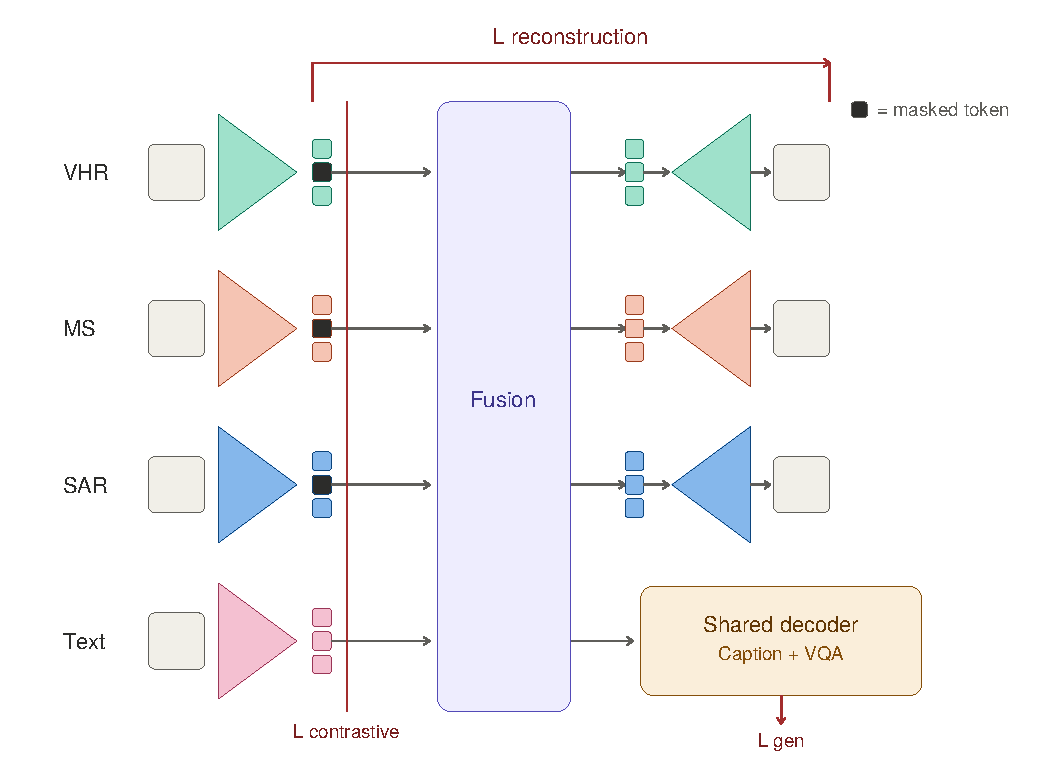
\includegraphics[width=0.95\textwidth]{images/multitask/quest_architecture_v2.pdf}
\caption{Overview of the QUEST architecture. Each modality is encoded
into patch tokens, a subset of which are masked (black squares) before
fusion, following the masked-patch-prediction strategy of
\textcite{astruc2024omnisat}. The fused representation feeds three
objectives: $\mathcal{L}_\text{reconstruction}$ predicts the masked
tokens' original content per visual modality,
$\mathcal{L}_\text{contrastive}$ aligns unmasked token embeddings
across all four modalities, and $\mathcal{L}_\text{gen}$ supervises
the shared captioning/VQA decoder. Only the objectives active in a
given configuration (Table~\ref{tab:chap6_configs}) are used during
training.}
\label{fig:chap6_architecture}
\end{figure}

\subsection{Multi-Modal Visual Encoders}
\label{sec:chap6_method_encoders}

Although the three visual modalities differ in spatial resolution,
spectral structure, and sensing physics, modality-specific encoders
convert each input into a sequence of $N = 100$ latent tokens in the
shared embedding space. This token count is the largest supported by
each modality's native resolution without upsampling (VHR
$1000\times1000$, SAR $200\times200$, multispectral $100\times100$),
balancing meaningful spatial footprint per token against fusion
compute.

\textbf{VHR RGB.} High-resolution RGB images are divided into
non-overlapping $100\times100$ patches. Each patch is flattened and
passed through a linear projection layer into the shared embedding
dimension, producing tokens $\{z^{\text{VHR}}_i\}_{i=1}^{N}$.

\textbf{Sentinel-2 multispectral.} Sentinel-2 inputs contain ten
spectral bands at heterogeneous native resolutions. A lightweight
convolutional stem (strided convolutions, pooling, and residual
blocks) harmonizes these bands and captures spectral interactions; the
resulting feature map is partitioned into $10\times10$ patches, each
projected into the shared embedding space to obtain tokens
$\{z^{\text{S2}}_i\}_{i=1}^{N}$.

\textbf{Sentinel-1 SAR.} SAR images are divided into $20\times20$
patches and passed through a linear projection layer, yielding tokens
$\{z^{\text{S1}}_i\}_{i=1}^{N}$.

\textbf{Shared transformer encoder.} For each modality
$m \in \{\text{VHR}, \text{S2}, \text{S1}\}$, a learnable class token
is prepended and modality-specific positional embeddings are added.
The resulting sequence is processed by a 6-layer transformer encoder
with 16 attention heads and an MLP expansion ratio of 4, producing
modality-aware latent representations
\[
\tilde{Z}^{m} = \text{TransformerEnc}(Z^{m}),
\]
which serve as the visual inputs to the fusion module.

\subsection{Text Encoder and Multi-Modal Fusion}
\label{sec:chap6_method_fusion}

Text inputs (captions or VQA queries) are encoded using a pretrained
T5 encoder. The resulting token embeddings are projected into the
shared $d = 256$ dimensional space and concatenated with the visual
tokens from all available modalities. The combined sequence is
processed by a transformer-based fusion module that uses self-attention
to integrate high-resolution spatial cues, multispectral information,
SAR patterns, and linguistic semantics. The output of this module,
denoted $F$, forms a unified representation supporting both contrastive
learning and generative decoding.

\subsection{Cross-Modal Contrastive Learning}
\label{sec:chap6_method_contrastive}

To enforce semantic consistency across modalities, two contrastive
objectives are used.

\textbf{Global image-text alignment.} For each visual modality $m$, a
pooled embedding is obtained by mean-pooling over its patch tokens,
denoted $g^{m}$, and a pooled text embedding $g^{\text{text}}$ is
obtained by mean-pooling over the caption tokens. A separate InfoNCE
term is computed per modality and summed, bringing matched image-text
pairs closer while pushing mismatched pairs apart, with a learned
temperature $\tau$:
\[
\mathcal{L}_{\text{global}} = \sum_{m} \left[ -\frac{1}{B} \sum_{i=1}^{B}
\log \frac{\exp(\text{sim}(g^{m}_i, g^{\text{text}}_i)/\tau)}
{\sum_{j=1}^{B} \exp(\text{sim}(g^{m}_i, g^{\text{text}}_j)/\tau)} \right].
\]
 
\textbf{Cross-modal visual alignment.} When resolutions differ,
correspondences are defined in the normalized spatial coordinate
system of the image: each patch token is associated with the center
coordinates of its receptive field, normalized to $[0,1]^2$. For two
modalities $m_1 \neq m_2$, each patch of $m_1$ is matched to the
geographically closest patch center of $m_2$, yielding a one-to-one or
one-to-many correspondence depending on resolution, without requiring
external registration beyond the co-registered imagery already
provided by TAMMI. The loss is
\[
\mathcal{L}_{\text{local-vis}} = -\frac{1}{B} \sum_{i}
\log \frac{\exp(\text{sim}(z^{m_1}_i, z^{m_2}_i)/\tau)}
{\sum_{k} \exp(\text{sim}(z^{m_1}_i, z^{m_2}_k)/\tau)}.
\]

\subsection{Visual Reconstruction}
\label{sec:chap6_method_reconstruction}

To prevent the shared representation from collapsing to purely
semantic features, each visual modality is equipped with a
reconstruction head trained via masked patch prediction. Concretely,
tokens across the three visual modalities are masked jointly, before
text tokens are concatenated, so that text is never masked and always
provides an unmasked conditioning signal: for each sample, a random
subset of visual token positions is selected via per-sample shuffling
(sorting random noise and keeping the first $\lfloor L(1-r)\rfloor$
positions, where $L$ is the total number of visual tokens and $r =
0.5$ is the masking ratio), and each masked position is replaced by a
shared, learned mask token rather than being removed from the
sequence or zeroed out.
The corresponding decoder $D_m$ is then trained to predict the
original patch content $\hat{x}^{m}_i$ for the masked tokens from the
fused representation, supervised with an $\ell_2$ loss:
\[
\mathcal{L}_{\text{rec}} = \sum_{m} \sum_{i \in \mathcal{M}^m}
\| \hat{x}^{m}_i - x^{m}_i \|_2^2,
\]
where $\mathcal{M}^m$ denotes the set of masked token indices for
modality $m$. Masking, rather than reconstructing every token
unconditionally, forces the decoder to rely on cross-modal and
spatial context propagated through the fusion module rather than
trivially copying each token's own visual encoding forward. For
modalities undergoing learned downsampling (Sentinel-2), the decoder
uses pooling indices from the encoder to restore spatial structure.
This is the objective ablated in
Section~\ref{sec:chap6_experiments} between the "w/ reco" and "w/o
reco" configurations.

\subsection{Captioning and Visual Question Answering}
\label{sec:chap6_method_decoding}

The fused representation $F$ is projected to the T5 hidden dimension
and used as encoder-side context for a T5 autoregressive decoder. The
decoder attends jointly to all visual and textual tokens via
cross-attention and generates either a caption or a VQA answer. A
single decoder is shared across both tasks, so that any transfer
between captioning and VQA is a property of the shared decoder rather
than of two independently trained heads, matching the study's goal of
measuring whether such transfer occurs rather than assuming it by
architectural construction.

\subsection{Total Loss}
\label{sec:chap6_method_loss}

The full training objective combines all components:
\[
\mathcal{L} = \lambda_{\text{global}} \mathcal{L}_{\text{global}}
+ \lambda_{\text{local-vis}} \mathcal{L}_{\text{local-vis}}
+ \lambda_{\text{rec}} \mathcal{L}_{\text{rec}}
+ \lambda_{\text{gen}} \mathcal{L}_{\text{gen}},
\]
where $\mathcal{L}_{\text{gen}}$ is the standard autoregressive
cross-entropy loss for captioning and VQA. Each of
$\lambda_{\text{rec}}$, and the presence of captioning versus VQA data
in $\mathcal{L}_{\text{gen}}$, is set to zero for the corresponding
ablated configuration in the study that follows, rather than requiring
separately trained architectures per configuration.

\section{Experimental Study}
\label{sec:chap6_experiments}

This section reports the four-configuration study motivated in
Section~\ref{sec:chap6_intro}. Section~\ref{sec:chap6_setup} defines
the four configurations and the evaluation protocol.
Section~\ref{sec:chap6_results} reports captioning and VQA metrics
across all four. Section~\ref{sec:chap6_results} examines individual examples in detail. Section~\ref{sec:chap6_discussion} discusses
these results, what they establish about the value of joint
training.

\subsection{Experimental Setup}
\label{sec:chap6_setup}

Four training configurations are compared, each obtained by enabling
or disabling terms of $\mathcal{L}$ (Section~\ref{sec:chap6_method_loss})
rather than by training separate architectures:

\begin{itemize}
\item \textbf{w/ reco}: the full model, trained with reconstruction,
contrastive alignment, captioning, and VQA jointly.
\item \textbf{w/o reco}: identical to \textbf{w/ reco} but with
$\lambda_{\text{rec}} = 0$, isolating the contribution of the
reconstruction objective specifically.
\item \textbf{VQA only}: $\mathcal{L}_{\text{gen}}$ restricted to VQA
and $\lambda_{\text{rec}} = 0$, with $\mathcal{L}_{\text{global}}$ and
$\mathcal{L}_{\text{local-vis}}$ still active; the single-task
baseline for VQA with respect to the generative and reconstruction
objectives specifically, though not a purely single-objective model.
\item \textbf{Caption only}: $\mathcal{L}_{\text{gen}}$ restricted to
captioning and $\lambda_{\text{rec}} = 0$, with $\mathcal{L}_{\text{global}}$
and $\mathcal{L}_{\text{local-vis}}$ still active; the single-task
baseline for captioning with respect to the generative and
reconstruction objectives specifically, though not a purely
single-objective model.
\end{itemize}

Table~\ref{tab:chap6_configs} summarizes which terms of
$\mathcal{L}$ are active in each configuration.

\begin{table}[ht]
\centering
\small
\caption{Loss terms active in each of the four training
configurations compared in this study. $\mathcal{L}_\text{global}$ and
$\mathcal{L}_\text{local-vis}$ are active in every configuration; only
$\mathcal{L}_\text{rec}$ and the task restriction on $\mathcal{L}_\text{gen}$
are ablated.}
\label{tab:chap6_configs}
\begin{tabular}{lccccc}
\toprule
\textbf{Configuration} & $\mathcal{L}_{\text{global}}$ & $\mathcal{L}_{\text{local-vis}}$ & $\mathcal{L}_{\text{rec}}$ & $\mathcal{L}_{\text{gen}}$ (caption) & $\mathcal{L}_{\text{gen}}$ (VQA) \\
\midrule
w/ reco       & \checkmark & \checkmark & \checkmark & \checkmark & \checkmark \\
w/o reco      & \checkmark & \checkmark &            & \checkmark & \checkmark \\
VQA only      & \checkmark & \checkmark &            &            & \checkmark \\
Caption only  & \checkmark & \checkmark &            & \checkmark &            \\
\bottomrule
\end{tabular}
\end{table}
All four configurations are trained on the same TAMMI splits
(Chapter~\ref{chap:tammi}, Section~\ref{sec:chap5_splitting}), extended
with the captions described in Section~\ref{sec:chap6_dataset}. All
models are optimized with Adam~\cite{kingma2015adam} at a learning
rate of $10^{-6}$ (no weight decay), with a
plateau-based learning rate decay scheduler (factor 0.1, patience 10 epochs)
monitoring validation loss, trained for a minimum of 14 and a maximum
of 20 epochs, and a batch
size of 16 per step. For the non-ablated terms of $\mathcal{L}$
(Section~\ref{sec:chap6_method_loss}), $\lambda_\text{rec} = 1.0$,
$\lambda_\text{local-vis} = 0.04$, and $\lambda_\text{global} = 0.18$.
Captioning is evaluated with ROUGE-1 and ROUGE-L, and with BERTScore
computed at four similarity thresholds (60, 70, 80, 90) to assess how
performance degrades as the required similarity to the reference
caption becomes stricter. VQA is evaluated with overall accuracy and with the
same BERTScore-threshold protocol applied to the generated answer text.
\subsection{Quantitative Results}
\label{sec:chap6_results}

Table~\ref{tab:chap6_captioning} reports captioning metrics and
Table~\ref{tab:chap6_vqa} reports VQA metrics across all four
configurations.

\begin{table}[ht]
\centering
\small
\caption{Captioning results across the four training configurations.
ROUGE scores are reported directly; BERTScore is reported as the
fraction of generated captions exceeding each similarity threshold.}
\label{tab:chap6_captioning}
\begin{tabular}{lcccc}
\toprule
\textbf{Metric} & \textbf{w/ reco} & \textbf{w/o reco} & \textbf{VQA only} & \textbf{Caption only} \\
\midrule
ROUGE-1 & 0.5055 & \textbf{0.5159} & -- & 0.5032 \\
ROUGE-L & 0.4173 & \textbf{0.4227} & -- & 0.4183 \\
BERTScore @ 60 & 1.0000 & 1.0000 & -- & 1.0000 \\
BERTScore @ 70 & 0.9997 & \textbf{1.0000} & -- & \textbf{1.0000} \\
BERTScore @ 80 & 0.9871 & \textbf{0.9891} & -- & 0.9873 \\
BERTScore @ 90 & 0.2288 & 0.2344 & -- & \textbf{0.2355} \\
\bottomrule
\end{tabular}
\end{table}

\begin{table}[ht]
\centering
\small
\caption{VQA results across the four training configurations.
BERTScore is reported as the fraction of generated answers exceeding
each similarity threshold.}
\label{tab:chap6_vqa}
\begin{tabular}{lcccc}
\toprule
\textbf{Metric} & \textbf{w/ reco} & \textbf{w/o reco} & \textbf{VQA only} & \textbf{Caption only} \\
\midrule
Overall Accuracy & 0.5613 & 0.5619 & \textbf{0.5769} & -- \\
BERTScore @ 60 & 0.9987 & 0.9982 & \textbf{0.9999} & -- \\
BERTScore @ 70 & 0.9525 & \textbf{0.9555} & 0.9550 & -- \\
BERTScore @ 80 & 0.8572 & 0.8558 & \textbf{0.8644} & -- \\
BERTScore @ 90 & 0.7571 & 0.7470 & \textbf{0.7589} & -- \\
\bottomrule
\end{tabular}
\end{table}

On captioning, w/o reco slightly outperforms w/ reco on both ROUGE
metrics (0.5159 vs.\ 0.5055 ROUGE-1; 0.4227 vs.\ 0.4173 ROUGE-L) and
tracks close to the Caption-only single-task baseline across all six
metrics, with no metric where w/ reco is the best of the three. On
VQA, VQA-only outperforms both multi-task configurations on every
metric, most notably on overall accuracy (0.5769 vs.\ 0.5613--0.5619).
Neither task, at the level of these aggregate metrics, shows joint
training outperforming its corresponding single-task baseline.

\subsection{Qualitative Analysis}
\label{sec:chap6_qualitative}

Aggregate metrics average over all question types and caption content
uniformly, which can mask effects specific to a particular question
type or scene. This section examines four individual examples, each
selected to test a specific aspect of the quantitative results above:
a failure shared across all configurations, a case where joint
training succeeds despite losing on aggregate, a captioning comparison
that stress-tests what BERTScore actually rewards, and the
reconstruction quality underlying $\mathcal{L}_\text{rec}$ itself.

\begin{figure}[ht]
\centering
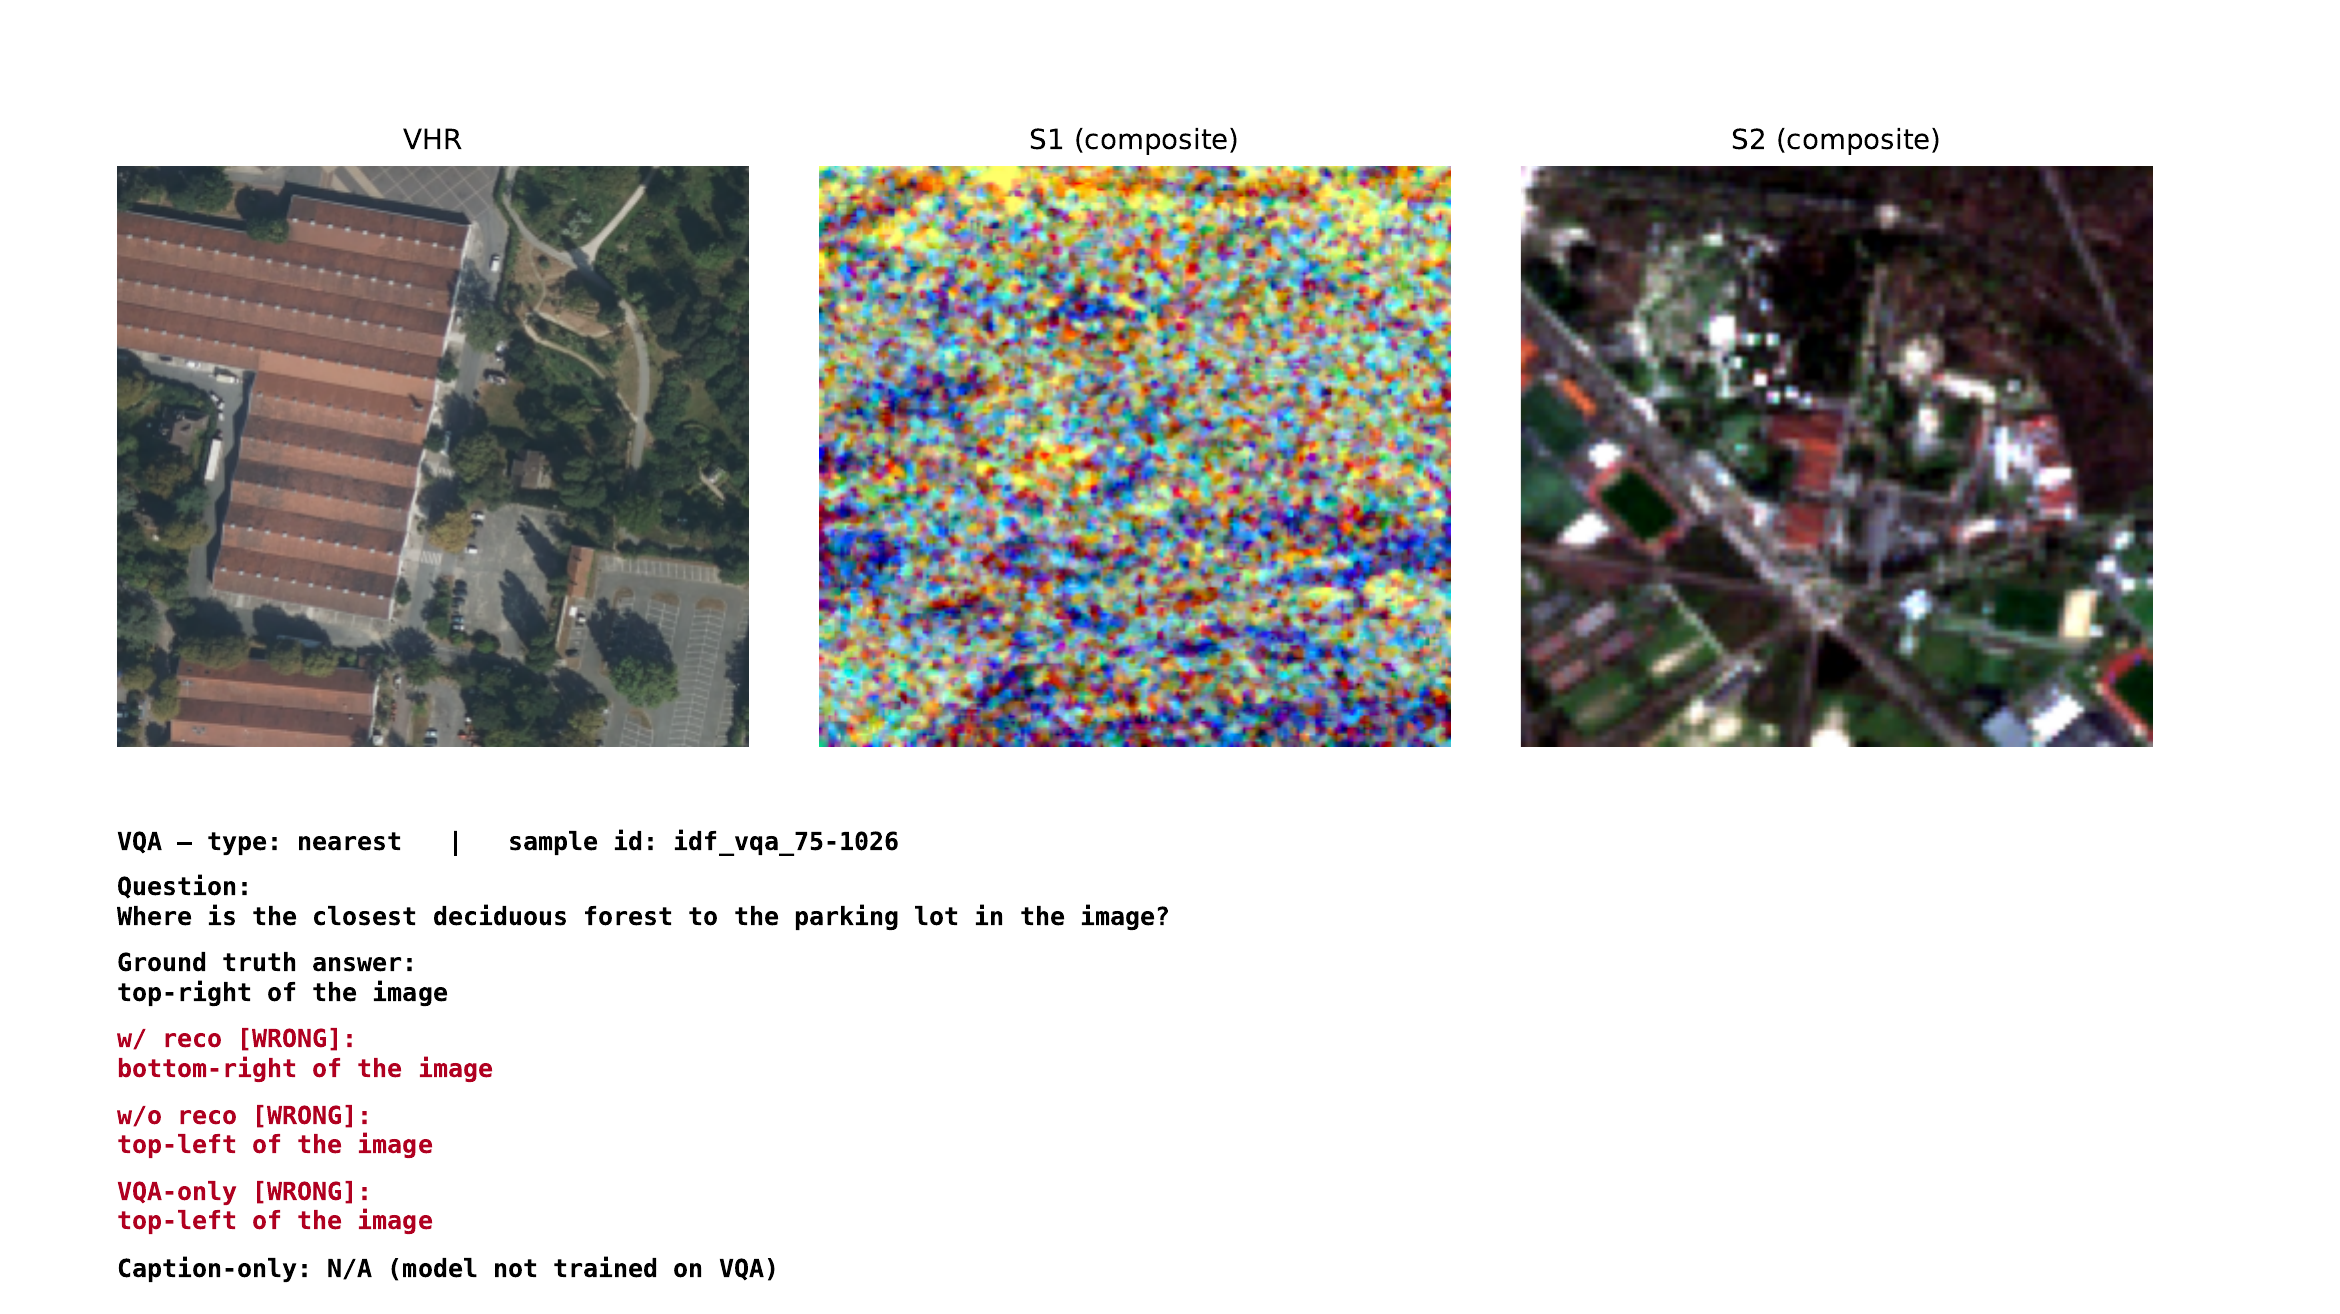
\includegraphics[width=0.85\textwidth]{images/multitask/qual_vqa_failure.png}
\caption{A \textit{nearest} question
on which all configurations answer incorrectly, converging on
different but equally wrong directions.}
\label{fig:chap6_qual_vqa_fail}
\end{figure}

In Figure~\ref{fig:chap6_qual_vqa_fail}, all configurations answer this \textit{nearest} question
incorrectly, each converging on a different wrong direction rather
than a shared one. This is consistent with two compounding
difficulties rather than a single cause: ambiguity in what "nearest"
refers to when several candidate objects are plausible, and the
resolution limits on resolving fine spatial relations discussed
throughout this thesis. Since the failure is shared across every
configuration, including VQA-only, it is not attributable to
multi-task training specifically, and is better read as a property of
the question type itself.

\begin{figure}[ht]
\centering
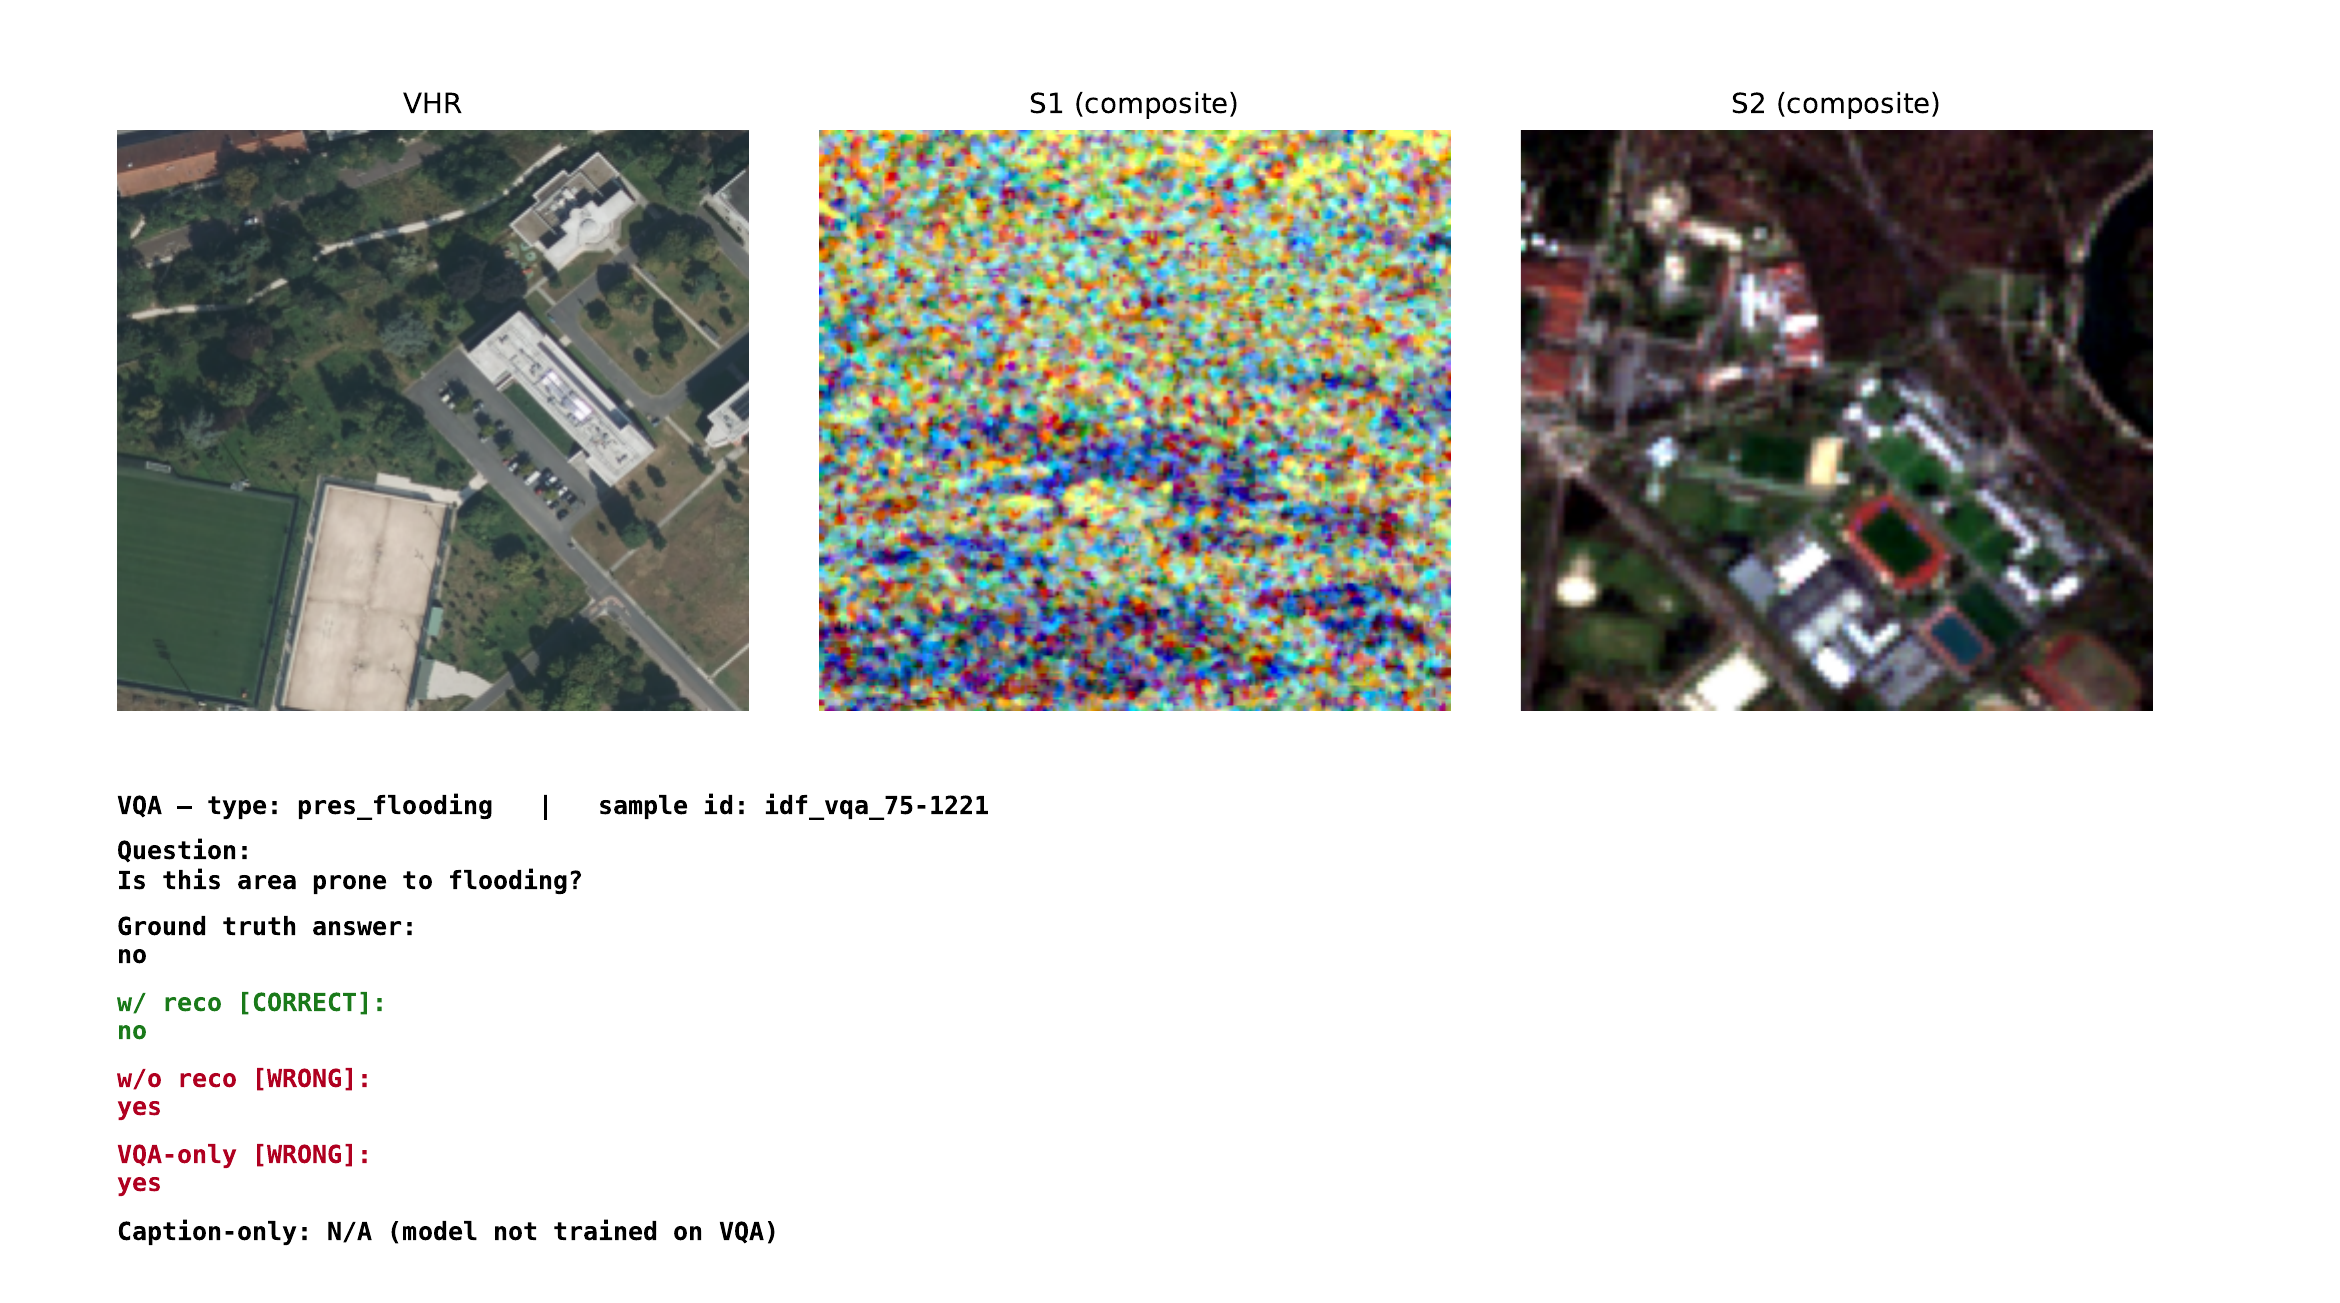
\includegraphics[width=0.85\textwidth]{images/multitask/qual_vqa_success.png}
\caption{A \textit{Flooding Presence} question on which the full multi-task model (w/
reco) answers correctly while both w/o reco and VQA-only answer
incorrectly.}
\label{fig:chap6_qual_vqa_success}
\end{figure}

The example in Figure~\ref{fig:chap6_qual_vqa_success} is a direct counter-example to the aggregate accuracy
result in Table~\ref{tab:chap6_vqa}: although VQA-only wins on
average, here it is the full multi-task model that answers correctly
while the single-task baseline does not. A single example cannot
establish how common this pattern is, but it demonstrates that the
aggregate result is compatible with joint training helping on specific
question types, rather than ruling this out.

\begin{figure}[ht]
\centering
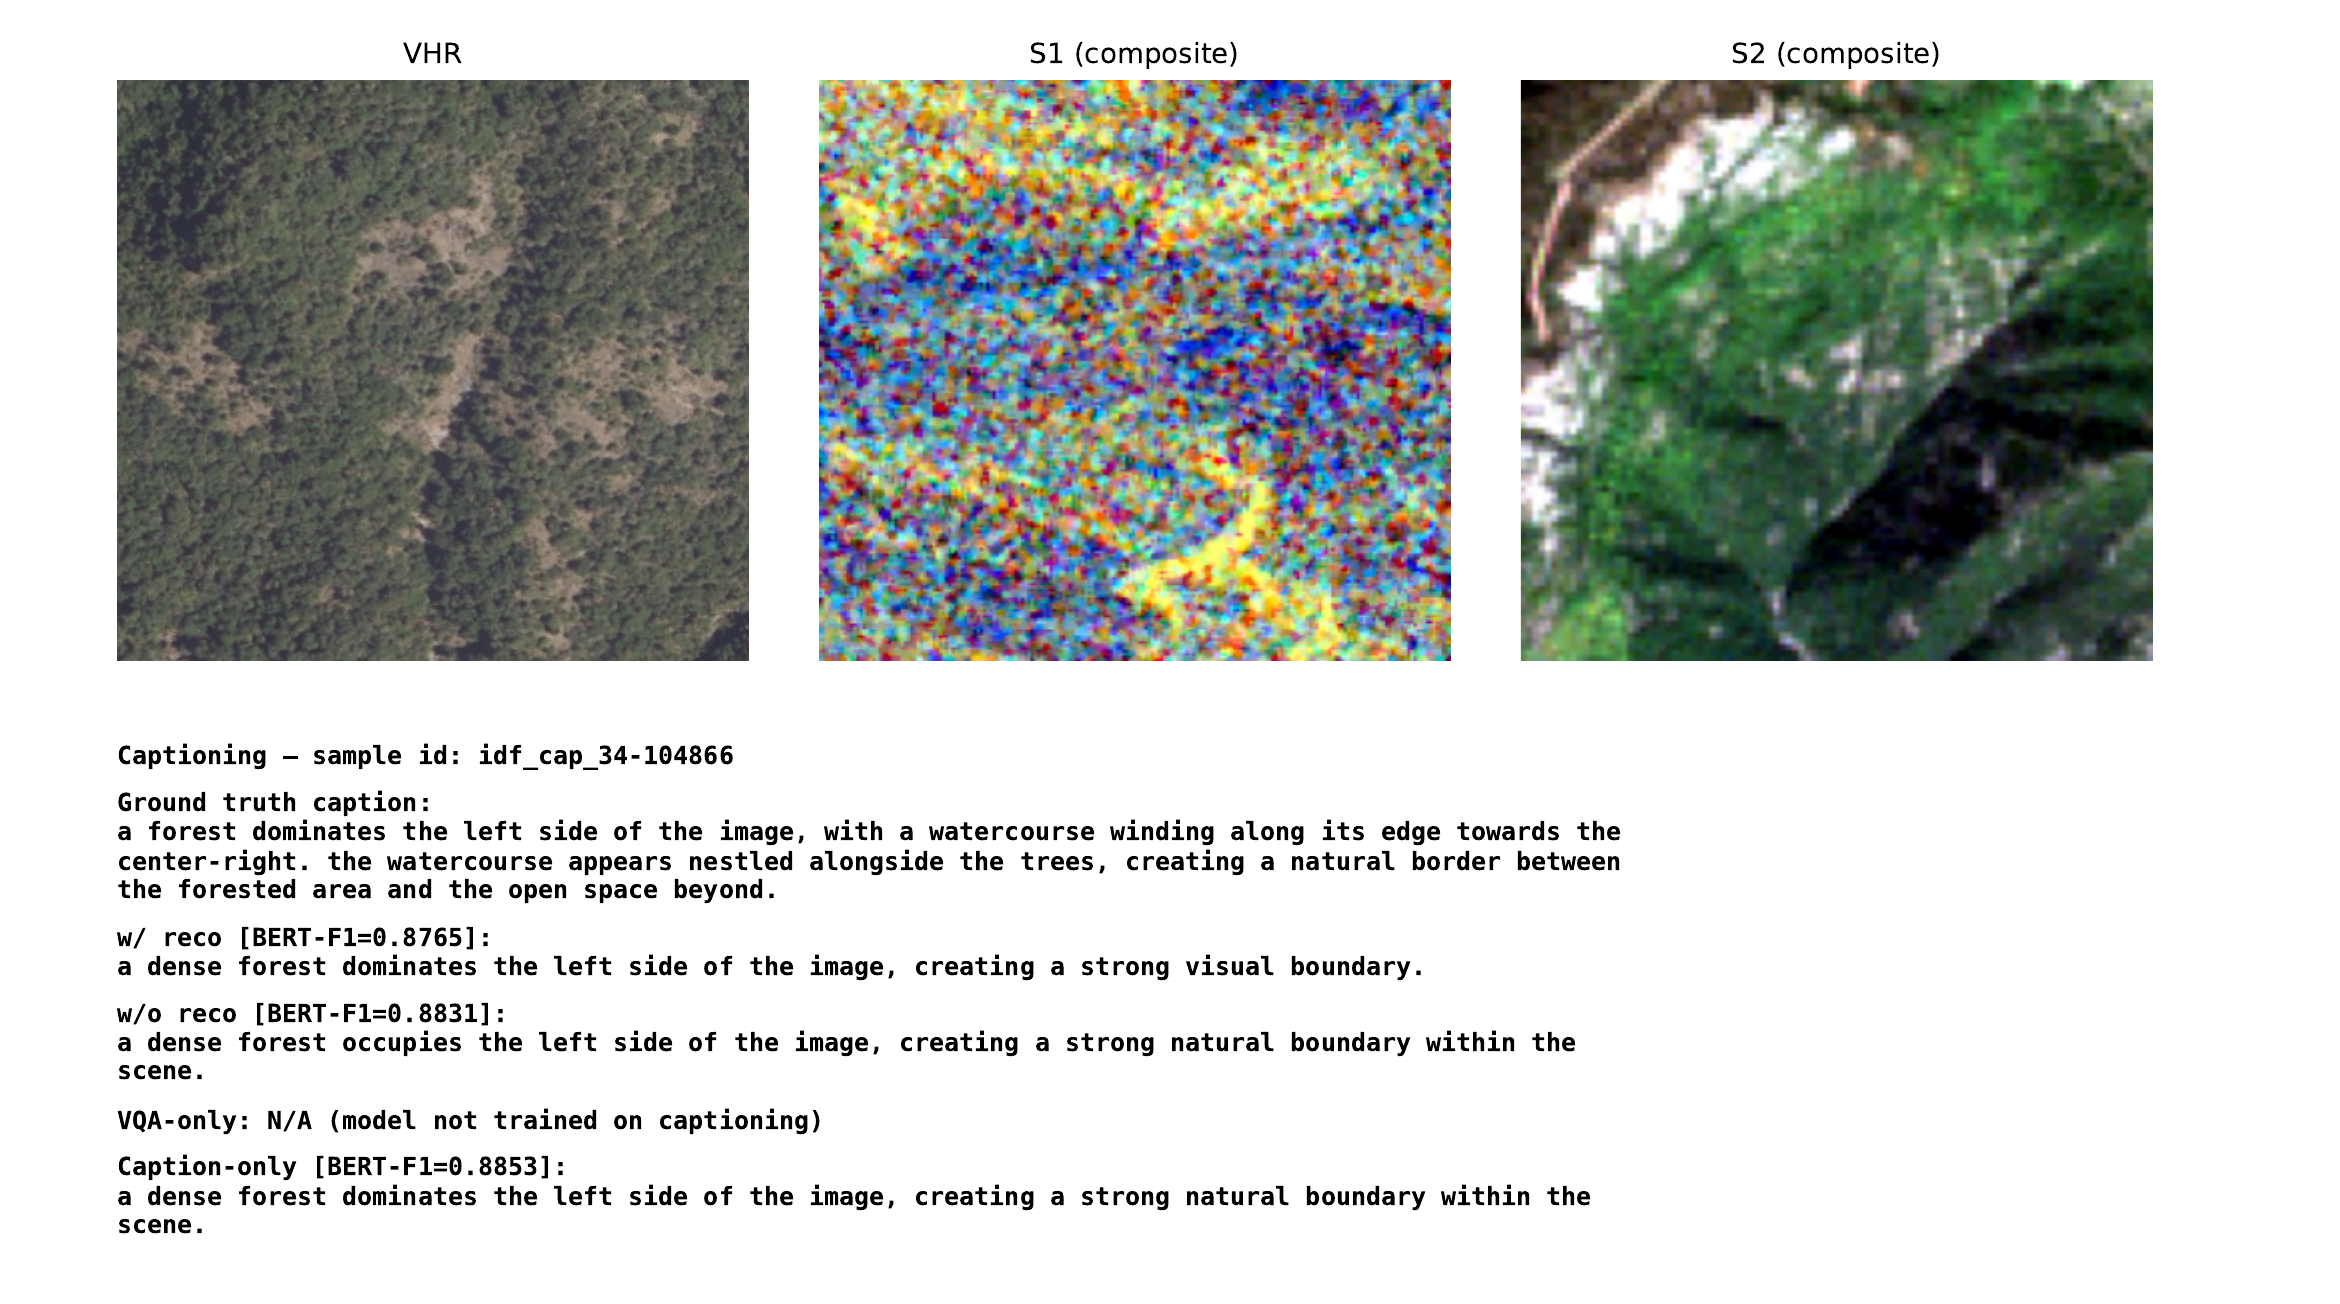
\includegraphics[width=0.85\textwidth]{images/multitask/qual_captioning.png}
\caption{Generated captions from each captioning-capable configuration
for the same VHR/SAR/multispectral triplet, alongside the ground-truth caption and
each configuration's BERTScore F1.}
\label{fig:chap6_qual_caption}
\end{figure}

In the example of Figure~\ref{fig:chap6_qual_caption} all three configurations correctly identify the dominant forest and
describe it as forming a boundary, but none mentions the watercourse
that the ground-truth caption explicitly describes as running along
the forest's edge, despite each scoring above 0.87 BERTScore F1. This
illustrates a limitation of embedding-based similarity metrics
discussed in Section~\ref{sec:chap6_setup}: a caption can omit a
salient detail entirely and still score highly if the retained content
is semantically close to the reference. The three configurations are,
by this metric, nearly indistinguishable on this example, despite
omitting the same real piece of information.

\begin{figure}[ht]
\centering
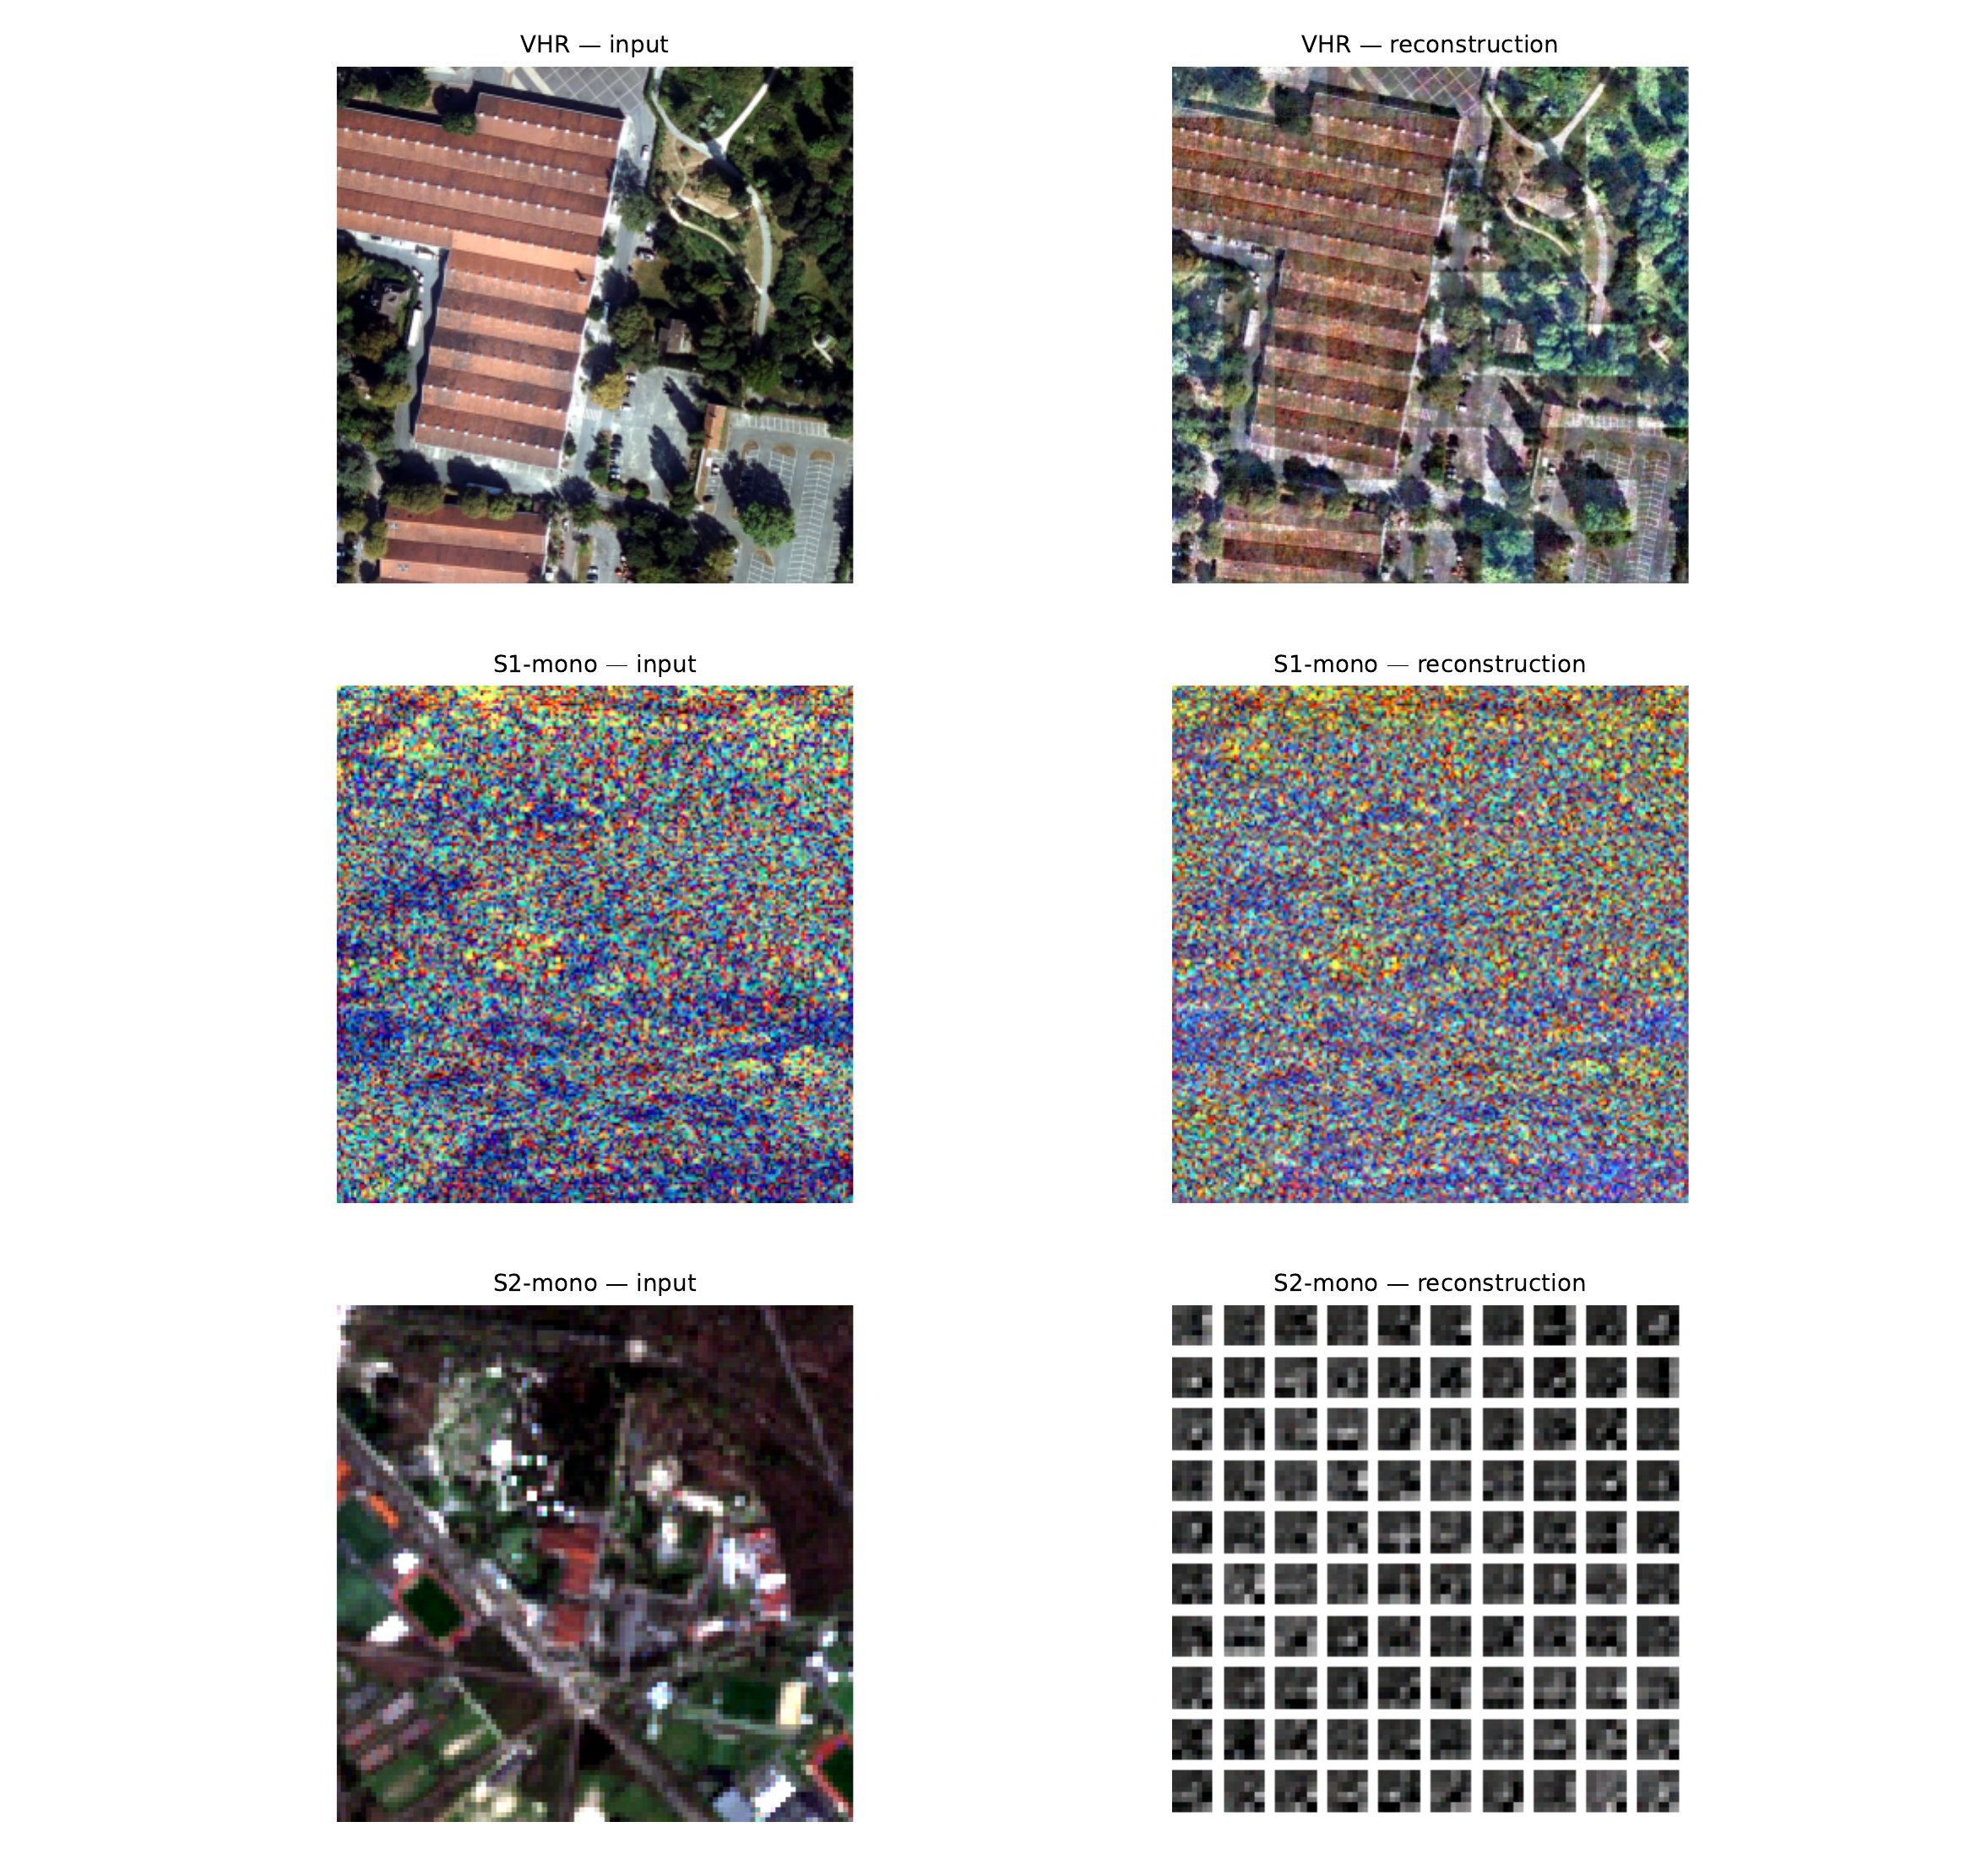
\includegraphics[width=0.85\textwidth]{images/multitask/qual_reconstruction.png}
\caption{Input and reconstructed patches for the VHR, SAR, and
multispectral modalities of a single TAMMI sample.}
\label{fig:chap6_qual_reco}
\end{figure}

In Figure~\ref{fig:chap6_qual_reco}, the VHR reconstruction recovers recognizable structure (building
outlines, road layout) closely matching the input; the SAR
reconstruction reproduces plausible speckle statistics, though a
pixel-level ground-truth comparison is not visually meaningful for
SAR. The multispectral reconstruction, however, shows a consistent,
spatially localized region of degraded content within each individual
patch, in the same relative position across patches and samples
regardless of the patch's actual content, unlike the ground truth's
dark regions, which vary in position with scene content as expected.
Isolating individual, unstitched patches traced this pattern to the
level of a single patch, ruling out stitching order and display-side
stretching as causes. It is consistent with information loss from
unpooling operations' max-pooling indices being systematically biased
at the very small ($10\times10$) patch resolution used for this
modality, though confirming this would require further architectural
investigation beyond the scope of this study.

\subsection{Discussion}
\label{sec:chap6_discussion}

Taken together, these results echo the RS-LLaVA finding already
discussed in Section~\ref{sec:rw-captioning-challenges}: single-task
training matches or exceeds multi-task training on both tasks studied
here, and reconstruction specifically does not measurably help
captioning. This is consistent with, rather than contradicting, this
chapter's framing: the premise motivating datasets and models that
combine these tasks is that joint training helps, and the aggregate
metrics above do not support that premise for either task. Combined
with the RS-LLaVA result, this provides a second, independent
measurement, on a different dataset, architecture, and task
combination, of the same pattern: assumed multi-task synergy in RS
vision-language models does not straightforwardly hold once measured
directly.

The reconstruction finding (Figure~\ref{fig:chap6_qual_reco}) offers a
partial, modality-specific explanation for this. Since
$\mathcal{L}_\text{rec}$ sums over all three visual modalities jointly
(Section~\ref{sec:chap6_method_reconstruction}), a modality-specific
weakness in the multispectral reconstruction would dilute the
aggregate reconstruction signal without being visible in the aggregate
loss value alone, plausibly contributing to why enabling reconstruction
("w/ reco") did not translate into a measurable downstream benefit for
either task.

At the same time, this chapter's aggregate metrics do not, on their
own, rule out category-specific synergy: the flooding-question example
(Figure~\ref{fig:chap6_qual_vqa_success}) shows the full multi-task
model succeeding where the single-task baseline fails. A per-question-type breakdown,
analogous to the one reported for MM-RSVQA in
Chapter~\ref{chap:tammi} and for the augmentation study in
Chapter~\ref{chap:llm_augmentation}, would clarify whether this
reflects a genuine category-specific effect or an isolated case, and
is a natural extension of this study, discussed further in
Section~\ref{sec:chap6_conclusion}.

\section{Conclusion and Limitations}
\label{sec:chap6_conclusion}

This chapter extended TAMMI with captions and introduced a unified
architecture combining cross-modal contrastive alignment, reconstruction,
and a shared generative decoder for captioning and VQA, then used it to
study, rather than assume, whether reconstruction and joint
captioning-VQA training improve performance on either task. At the
level of aggregate metrics, neither does: single-task training matches
or outperforms every multi-task configuration on both captioning and
VQA. This adds a second data point, alongside RS-LLaVA
(Section~\ref{sec:rw-captioning-challenges}), to the pattern that assumed
multi-task synergy in RS vision-language models does not straightforwardly
hold when measured directly.

\textbf{Limitations.} This study is conducted at the level of aggregate
metrics; a per-question-type breakdown, analogous to the one reported
for MM-RSVQA in Chapter~\ref{chap:tammi} and for the augmentation study
in Chapter~\ref{chap:llm_augmentation}, would clarify whether the
absence of synergy found here holds uniformly across question types or
masks category-specific effects, and is left for future work. Beyond
this, the study is conducted on a single dataset (TAMMI) and a single
architecture; whether the same pattern holds for other RS multi-task
combinations, or for architectures where reconstruction and generation
share more capacity than in the fusion design used here, remains open.
Finally, the multispectral reconstruction weakness identified in
Section~\ref{sec:chap6_discussion} was investigated only to the point
of localizing it, confirming the specific
mechanism, and addressing it, most plausibly by replacing the 
multispectral decoder's index-based upsampling with a learned upsampling stage, 
would require retraining and is left for future work.
%\chapter{CTCR-RS: Composed Temporal Change Retrieval in Remote Sensing}
\label{chap:ctcr}
\epigraph{\itshape  La volonté trouve, la liberté choisit. Trouver et choisir, c'est penser}{-- Victor Hugo}

\startcontents[chapters]
\printmyminitoc{
%	\lipsum[1]
}

% ============================================================
\section{Introduction}
\label{sec:chap6_intro}
% ============================================================
 
The preceding chapters addressed the problem of extracting
information from remote sensing imagery through visual
question answering: given an image and a question, produce
an answer. This formulation, while powerful, assumes that
the analyst already knows which location to look at and
simply wants to query its content. A complementary and
arguably more operationally critical problem is the inverse:
given a description of what one is looking for, find the
locations in a large archive that match it. This chapter
addresses this retrieval problem in the context of temporal
change, a information-rich and practically
relevant signals in Earth Observation archives.
 
Earth Observation satellites continuously accumulate imagery
of the same geographic locations at different points in time.
These archives have grown to a scale that makes manual
inspection infeasible: a single Sentinel-2 acquisition covers a swath width of
290\,km at resolutions ranging from 10 to 60\,m, and the
global archive now spans over a decade of bi-weekly
acquisitions. The ability to automatically retrieve locations
exhibiting a specific type of change, urban expansion,
deforestation, coastal erosion, or infrastructure construction,
from these archives is therefore a fundamental capability
for environmental monitoring, urban planning, disaster
response, and land-use policy. Earlier retrieval approaches rely either on visual queries 
alone (Content-Based Image Retrieval, CBIR), which cannot 
express semantic changes absent from the reference image, 
or on text-only queries (text-to-image retrieval), which 
require the analyst to exhaustively describe all expected 
changes from scratch, a burden that grows rapidly with 
scene complexity. Neither is fully adequate for the operational setting in 
which an analyst has already observed a set of changes and 
wishes to find locations exhibiting those same changes 
plus additional ones specified in natural language.

This chapter proposes a composed multi-modal query
formulation that addresses both limitations simultaneously.
Given a reference pair of bi-temporal images depicting an
observed set of land-cover changes, and a textual instruction
specifying additional changes to be composed with those
already observed, the task is to retrieve target image pairs
that exhibit the union of visual and textual changes (see Figure \ref{fig:chap6_task}). This
\textit{Composed Temporal Change Retrieval} (CTCR)
formulation is inspired by Composed Image
Retrieval~\cite{song2025survey}, which has demonstrated
strong performance for single images, and extends it to the
bi-temporal setting where the query is not a single image
but a pair encoding a temporal transition. To illustrate
the practical value of this formulation, consider an analyst
monitoring post-disaster recovery after a flood event. A
reference pair already captures the flooding itself: water
expansion, road submersion, and building damage. The analyst
wants to retrieve all archive locations where this same
flood pattern occurred but where recovery has additionally
begun. Describing this full composed query in pure text is
tedious and imprecise. With CTCR-RS, the analyst simply
provides the flood reference pair and specifies the recovery
changes as a short textual addition.
 
Despite the clear motivation, composed retrieval for
bi-temporal changes has not previously been explored.
Composed Image Retrieval methods operate on single-date
images and have no mechanism for encoding the temporal
change between two acquisitions.
\textcite{ventura2024covr} handle temporal sequences but
rely on continuous motion rather than the discrete
before/after land-cover transitions that characterize
satellite time series. Within remote sensing specifically, Hoxha et al. \cite{hoxha2025selfsupervised}
extend cross-modal retrieval to bi-temporal image pairs,
supporting both text-to-pair and pair-to-text directions.
Single-image CIR has been adapted
to remote sensing~\cite{psomas2024cir, wang2024scene,
yang2025language}, but cannot account for changes across
time.
 
To address this gap, this chapter introduces Composed
Temporal Change Retrieval in Remote Sensing (CTCR-RS). The
task is formally defined as follows: given a reference pair
$\mathcal{I}_\text{ref} = (I_1, I_2)$ depicting visual
changes $\mathcal{L}(\mathcal{I}_\text{ref})$, and a
textual instruction $\mathcal{C}_\text{text}$ specifying
additional changes, retrieve a target pair
$\mathcal{I}_\text{tar}$ such that:
\begin{equation}
    \mathcal{L}(\mathcal{I}_\text{tar}) =
    \mathcal{L}(\mathcal{I}_\text{ref}) \cup
    \mathcal{C}_\text{text}
    \label{eq:ctcr_task}
\end{equation}
To support this task, we construct the CTCR-RS dataset, the
first large-scale benchmark for composed change retrieval in
remote sensing, by normalizing free-form change captions from
two established change captioning datasets into a structured
14-class geospatial ontology, yielding 30,179 compositional
triplets. We establish two baseline architectures: UniCTCR,
which addresses the task through end-to-end latent
multi-modal fusion, and StageCTCR, which decomposes the
problem into an explicit semantic composition stage using
LLaVA-NeXT~\cite{liu2024llavanext} fine-tuned via
LoRA~\cite{hu2021lora}, followed by a domain-adapted
retrieval stage using a LoRA-adapted CLIP model. Our results
show that explicit staged decomposition consistently
outperforms implicit latent fusion, providing a strong
baseline and a set of insights for the community.
 
It is important to acknowledge upfront that the work
presented in this chapter is deliberately scoped and
preliminary. The CTCR-RS dataset is built from two datasets
covering urban land-cover changes in a limited number of
geographic regions, and the proposed architectures are
baselines rather than optimized systems. The long-term
vision of this work, however, is considerably more
ambitious: a general-purpose composed change retrieval system
capable of querying heterogeneous EO archives across diverse
geographic regions, change types, and sensor modalities,
enabling analysts to compose queries from any combination of
visual reference and natural language modification without
exhaustive description. This chapter establishes the task
definition, the evaluation framework, and the first evidence
that the problem is tractable, as a foundation for this
broader research agenda.
 
The remainder of this chapter is organized as follows.
Section~\ref{sec:chap6_rw} reviews related work on composed
retrieval, bi-temporal change understanding, and
vision-language models for Earth Observation.
Section~\ref{sec:chap6_dataset} describes the CTCR-RS task
formalization and dataset construction pipeline.
Section~\ref{sec:chap6_method} presents the UniCTCR and
StageCTCR architectures. Section~\ref{sec:chap6_experiments}
reports experimental results including ablation studies,
complexity analysis, and qualitative examples.
Section~\ref{sec:chap6_impact} discusses broader impact and
ethical considerations. Section~\ref{sec:chap6_conclusion}
concludes with limitations and perspectives.
 
\begin{figure}[ht]
    \centering
    % NOTE: insert Figure 1 from the main paper here
    % (task illustration: reference pair with visual changes,
    % text change query, retrieved target pair)
    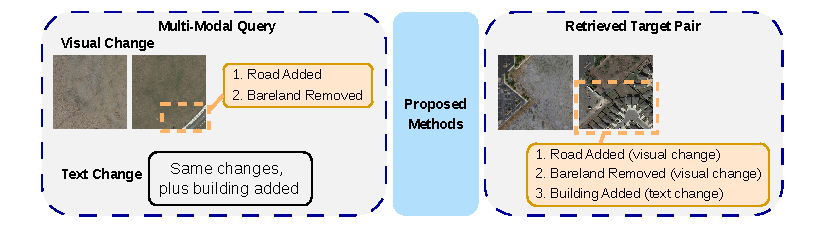
\includegraphics[width=\textwidth]{images/CTCR-RS/figure1-example-eccv.pdf}
    \caption{An example of the Composed Temporal Change
    Retrieval (CTCR-RS) task. Given a reference bi-temporal
    pair depicting two visual changes (Road Added, Bareland
    Removed) and a textual query specifying an additional
    change (Building Added), the system retrieves a target
    pair exhibiting all three changes.}
    \label{fig:chap6_task}
\end{figure}
 
% ============================================================
\section{Related Work}
\label{sec:chap6_rw}
% ============================================================
 
The related work covered in Chapter~\ref{chap:background}
addresses the broader foundations: general VQA and
vision-language architectures, RS image retrieval at the
conceptual level, and CLIP-based cross-modal alignment.
This section focuses on three aspects specific to this
chapter: composed retrieval for single images and video,
bi-temporal change understanding in remote sensing, and
vision-language models adapted for Earth Observation.
 
\subsection{Composed Image and Video Retrieval}
\label{sec:chap6_rw_cir}
 
Composed Image Retrieval (CIR) aims to retrieve a target
image given a visual reference and a textual modifier that
specifies how the target should differ from the
reference~\cite{song2025survey}. Supervised approaches
rely on cross-modal attention, dual-pathway architectures,
or modality fusion mechanisms~\cite{delmas2022artemis,
hosseinzadeh2020composed, huang2024dynamic, wen2024simple}.
To mitigate the scarcity of curated training triplets,
Zero-Shot CIR paradigms map visual concepts into language
token spaces via textual inversion~\cite{baldrati2023zero,
saito2023pic2word}, or caption the reference image using a
pretrained generative VLM and leverage an LLM to recompose
the caption based on the textual modifier~\cite{karthik2023vision}.
More recently, chain-of-thought reasoning has been used
to perform training-free zero-shot
composition~\cite{tang2025reason}.
 
CIR has been successfully adapted to the remote sensing
domain to refine single-image retrieval using textual
queries~\cite{psomas2024cir, wang2024scene, yang2025language}.
However, these methods operate on single-date images and
cannot account for changes occurring across time, motivating
the extension of CIR to the multi-temporal setting.
 
Composed Video Retrieval (CoVR) extends the CIR paradigm to
retrieve target videos based on reference clips and textual
modifiers~\cite{ventura2024covr, ventura2024covr2}. Recent
work explores fine-grained semantic alignment, feature
disentanglement, two-stage training, and pseudo-query
fine-tuning~\cite{gupta2025play, thawakar2024composed,
wu2025fine, zhang2024localizing}. However, CoVR models
continuous actions rather than discrete before/after
satellite states. While the visual structure superficially
resembles a short video (two frames), the semantic nature
of the transition is fundamentally different: bi-temporal
satellite imagery encodes land-use and land-cover change
rather than motion, and the temporal gap between
acquisitions is measured in months or years rather than
video frames. %Adapting CoVR by spatially stacking $I_1$
%and $I_2$ yields poor results on CTCR-RS (0.07 R@1
%zero-shot, 0.11 after fine-tuning), confirming that the
%paradigm transfer fails.
 
\subsection{Bi-Temporal Change Understanding in Remote Sensing}
\label{sec:chap6_rw_change}
 
Bi-temporal change understanding in remote sensing has been
primarily approached through Change Detection (CD) and
Change Captioning (CC). Change detection methods produce
pixel-level binary maps indicating changed versus unchanged
regions~\cite{peng2025deep}, while change captioning methods
generate natural language descriptions of the observed
transitions~\cite{liu2022levir, karaca2025secondcc}.
 
The LEVIR-CC dataset~\cite{liu2022levir} and the SECOND-CC
dataset~\cite{karaca2025secondcc} are the two primary
change captioning resources used in this chapter. LEVIR-CC
consists of bi-temporal aerial image pairs from urban areas
in Texas, USA, each annotated with five independent
human-authored change descriptions. SECOND-CC is a larger
and more diverse change captioning dataset covering a broader
range of urban changes across multiple geographic areas.
Both datasets provide the raw material for the CTCR-RS
pipeline.
 
Cross-modal text-image retrieval has been extended to the
temporal domain by~\cite{hoxha2025selfsupervised},
who propose self-supervised retrieval of time series based
on textual queries. However, this work restricts queries
to one modality only and does not support the composed multi-modal
formulation in which a visual reference pair provides the
base change context. The CTCR-RS task fills this gap by
combining a visual temporal reference with a textual
modifier in a single composed query.
 
\subsection{Vision-Language Models for Earth Observation}
\label{sec:chap6_rw_vlm}
 
Cross-modal retrieval for Earth Observation has undergone
significant progress through the adaptation of large
Vision-Language Models. Early methods bridge the semantic
gap between imagery and language using dual-stream networks
optimized via ranking losses~\cite{cheng2021deep,
yuan2022exploring}. More recently, VLMs such as
RemoteCLIP~\cite{liu2024remoteclip} and
GeoRSCLIP~\cite{zhang2024rs5m} have redefined the
state-of-the-art by leveraging contrastive learning over
massive datasets including RS5M~\cite{zhang2024rs5m},
RSITMD~\cite{RSITMD}, and RSICD~\cite{lu2017exploring}, achieving
robust modality alignment for image-to-text and
text-to-image retrieval.
 

However, existing RS VLMs are pretrained exclusively on
single-date image-text pairs, meaning their embedding spaces
are optimized for static scene description rather than
temporal change representation. While some general-purpose
VLMs can process multiple images as input, they are trained
predominantly on natural images and do not capture the
specific semantics of land-cover change in satellite
imagery. More recently, specialized RS frameworks such as
ChangeChat~\cite{deng2025changechat} and
DeltaVLM~\cite{deng2026deltavlm} have introduced
bi-temporal inputs and change-aware objectives, enabling
interactive change analysis and multi-turn question
answering over bi-temporal pairs. However, none of these
models are designed for the composed retrieval setting, in
which a bi-temporal visual reference and a textual modifier
must be jointly processed to retrieve a target pair
exhibiting the union of both changes. This chapter
introduces two architectures that address this gap:
UniCTCR and StageCTCR.

% ============================================================
\section{The CTCR-RS Task and Dataset}
\label{sec:chap6_dataset}
% ============================================================
 
\subsection{Task Formalization}
\label{sec:chap6_task}
 
Let $\mathcal{I} = (I_1, I_2)$ be a bi-temporal image pair
depicting land-use and land-cover change between two
acquisitions of the same geographic location. We define
$\mathcal{L}(\mathcal{I}) = \{c_1, c_2, \ldots, c_n\}$ as
the set of discrete semantic change labels present in the
pair, where each $c_i$ belongs to a standardized ontology
$\mathcal{O}$ described in
Section~\ref{sec:chap6_ontology}.
 
A CTCR-RS query is defined as a tuple
$(\mathcal{I}_\text{ref}, \mathcal{C}_\text{text})$, where
$\mathcal{I}_\text{ref}$ is a reference bi-temporal image
pair and $\mathcal{C}_\text{text}$ is a textual instruction
specifying additional changes to be composed with the
existing visual changes. The objective is to find a target
pair $\mathcal{I}_\text{tar}$ such that:
\begin{equation}
    \mathcal{L}(\mathcal{I}_\text{tar}) =
    \mathcal{L}(\mathcal{I}_\text{ref}) \cup
    \mathcal{C}_\text{text}
    \quad \text{where} \quad
    \mathcal{L}(\mathcal{I}_\text{ref}) \cap
    \mathcal{C}_\text{text} = \emptyset
\end{equation}
 
Critically, $\mathcal{I}_\text{ref}$ and
$\mathcal{I}_\text{tar}$ depict \textit{different}
geographic locations: the task retrieves archive locations
whose change pattern matches a composed visual-textual query,
analogous to reverse image search over change signatures
rather than tracking changes at a single fixed location over
time. This retrieval task is inherently one-to-many, as
multiple distinct geographic locations will inevitably share
the exact same ground-truth change label set
$\mathcal{L}(\mathcal{I}_\text{tar})$.
 
\subsection{Source Datasets and Domain Scoping}
\label{sec:chap6_sources}
 
The CTCR-RS dataset is constructed from two established
change captioning datasets: LEVIR-CC~\cite{liu2022levir}
and SECOND-CC~\cite{karaca2025secondcc}.
 
\textbf{LEVIR-CC}~\cite{liu2022levir} is a large-scale
remote sensing change captioning dataset built from the
LEVIR-CD change detection benchmark. It consists of 10,077
pairs of bi-temporal aerial images acquired over multiple
urban areas in Texas, USA, at a spatial resolution of
0.5\,m/pixel and a patch size of $256 \times 256$ pixels.
The temporal gap between acquisitions ranges from 5 to 14
years, capturing significant urban development changes.
Each image pair is annotated with five independent
human-authored captions describing the observed changes,
for a total of 50,385 captions. The predominant change
types are building construction and demolition, reflecting
the rapid urban expansion characteristic of the source
region.
 
\textbf{SECOND-CC}~\cite{karaca2025secondcc} is derived
from the SECOND semantic change detection dataset, which
covers six categories of land-cover objects (non-vegetated
ground surface, tree, low vegetation, water, buildings, and
playgrounds) across multiple cities in China. The dataset
contains 6 041 bi-temporal image pairs at $256 \times 256$
pixel resolution, each annotated with five human-authored
change captions, for a total of 30,205 captions. 
 
Both datasets share the key property of providing five
independent human-authored captions per image pair, which
is critical for the robustness of the label extraction
pipeline: redundant descriptions from multiple annotators
allow the LLM to cross-validate change labels and reduce
the impact of individual annotator errors or omissions, as
discussed in Section~\ref{sec:chap6_audit}.
 
 
A third publicly available dataset, RSCC~\cite{chen2025rscc},
covers disaster-related changes including floods,
earthquakes, and wildfires. While the automated curation
pipeline described below is general and could in principle
be applied to RSCC, this dataset covers a fundamentally
different semantic domain from the urban land-cover changes
in LEVIR-CC and SECOND-CC. We intentionally scope this
first benchmark to the urban domain to establish a clean,
controlled evaluation setting with a consistent change
ontology before extending to multi-domain scenarios.
Extending the CTCR-RS pipeline to disaster-related or
rural change datasets is an explicit direction for future
work.
 
\subsection{Caption Synthesis and Label Extraction}
\label{sec:chap6_extraction}
 
The first challenge in constructing CTCR-RS is transforming
the five heterogeneous, free-form human captions associated
with each image pair into a consistent set of structured
change labels. We employ Gemma~3~\cite{gemma2025} as a
semantic mapper, using a Chain-of-Thought (CoT) prompting
strategy to simultaneously synthesize redundant descriptions
and extract a normalized set of change labels.
 
The extraction proceeds in six reasoning steps: (1) object
analysis: listing all objects mentioned across the five
captions; (2) change type analysis: identifying all types
of changes described; (3) unique information extraction:
merging paraphrases and removing redundancy; (4) spatial
analysis: identifying where changes occur within the
image; (5) synthesis: combining the most important
elements into a single concise caption; (6) normalization, outputting a JSON array of object-change pairs. The full
prompt used for this stage is as follows:
 
\begin{quote}
\small
\textbf{System:} You are an expert in analyzing satellite
image changes using systematic reasoning.
 
\textbf{User:} Analyze the following 5 captions describing
a satellite image change for \{filename\}:
\{captions\_text\}
 
Follow these steps to reason through the changes:
 
STEP 1 -- OBJECT ANALYSIS: List all objects mentioned.
 
STEP 2 -- CHANGE TYPE ANALYSIS: List all types of changes.
 
STEP 3 -- UNIQUE INFORMATION EXTRACTION: Merge paraphrases,
remove redundancy, and list all distinct pieces of
information.
 
STEP 4 -- SPATIAL ANALYSIS: Where do changes occur?
 
STEP 5 -- SYNTHESIS: Combine the most important elements
into one concise caption.
 
STEP 6 -- NORMALIZED CHANGES: From the above, output a
JSON array of object-change pairs.
 
\textbf{Rules:}
\begin{itemize}
    \item Use common sense to normalize object names to a
    standard form (e.g., ``gray structures'' $\to$
    ``building'', ``soil area'' $\to$ ``bareland'').
    \item Use common sense to normalize change types (e.g.,
    ``constructed'' $\to$ ``added'', ``demolished'' $\to$
    ``removed'').
    \item If the change involves replacing one class with
    another (e.g., bareland with vegetation), treat it as
    two operations: \{object: ``bareland'', change:
    ``removed''\} and \{object: ``vegetation'', change:
    ``added''\}.
    \item For ``X replaced Y'' or ``X replaces Y'': output
    \{object: Y, change: ``removed''\} and \{object: X,
    change: ``added''\}.
    \item For "X is replaced by Y": output {object: X, change: "removed"} 
  and {object: Y, change: "added"}.
\item Never output objects with "no change" — omit unchanged objects 
entirely.
\item Ignore location words and process words.
\item Only include pairs explicitly stated in the captions.
\end{itemize}
\textbf{Final Optimal Caption}:
One mid-sized caption around 25 words summarizing the main scene 
differences, not listing every single change

\textbf{Normalized Changes}:
JSON array of {"object": "...", "change": "..."}
\end{quote}
 
A critical design choice in this stage is the decomposition
of inter-class transitions. For changes involving a semantic
class transition (e.g., a forest cleared for an excavation
site), the model is instructed to decompose the event into
two independent operations: Removal, representing the
disappearance of the initial state, and Addition,
representing the appearance of the final state. This ensures
that the resulting change sets correctly capture both sides
of a transition, supporting compositional matching in
retrieval.
 
\subsection{Taxonomy and Change Ontology}
\label{sec:chap6_ontology}
 
The initial extraction pass produces normalized but still
potentially inconsistent labels. A second pass with
Gemma~3 enforces a controlled vocabulary of 14
standardized geospatial change types, defined over six
broad change categories and three change types:
 
\textbf{Change categories:} Building, Bareland, Water,
Vehicle, Vegetation, Road.
 
\textbf{Change types:} Added, Removed, Replaced (the latter
specifically accounts for intra-class transitions such as
infrastructure upgrades or building redevelopments).
 
This yields $6 \times 3 = 18$ theoretical combinations,
reduced to 14 in practice as Replaced is only meaningful
for infrastructure classes (Building, Road). Fine-grained
object descriptors are consolidated into these broad
macroscopic categories (e.g., ``villa'', ``apartment'', and
``factory'' all map to Building), while action verbs are
normalized to the three allowed change types (e.g.,
``constructed'', ``erected'', ``built'' all map to Added).
 The full prompt used for this normalization stage is as
follows:
 
\begin{quote}
\small
\textbf{System:} You are an expert in satellite image change
analysis.
 
\textbf{User:} Here are captions and their current
normalized\_changes for multiple entries:
\{batch\_json\}
 
Your task: review and correct ONLY the
``normalized\_changes'' field for each entry.
 
\textbf{Ontology:}
\begin{itemize}
    \item Broad types: building, vegetation, road, water,
    vehicle, bareland.
    \item Subtypes: any descriptive term is allowed.
    \item Allowed change values: added, removed, replaced.
\end{itemize}
 
\textbf{Rules:}
\begin{enumerate}
    \item Verify that all changes are consistent with
    captions.
    \item Correct mislabeled objects to match the ontology.
    \item Merge duplicate changes (same broad type + same
    change type).
    \item Normalize all free-text change values into the
    allowed set above.
    \item Drop any single change with ``no\_change''.
    \item Output must be valid JSON only.
\end{enumerate}
\end{quote}

\begin{figure}[ht]
    \centering
    % NOTE: insert Figure 2 from the main paper here
    % (full dataset curation pipeline figure)
    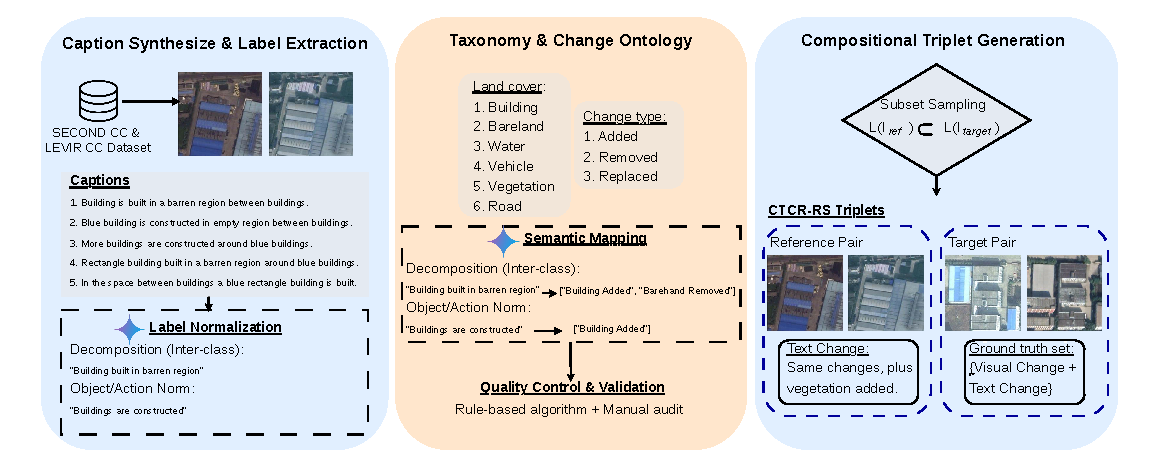
\includegraphics[width=\textwidth]{images/CTCR-RS/figure2-dscuration-eccv.pdf}
    \caption{The CTCR-RS dataset curation pipeline from raw
    captions to composed retrieval triplets. Raw captions
    from LEVIR-CC and SECOND-CC are processed through
    caption synthesis and label extraction (Stage~1),
    taxonomy normalization (Stage~2), quality control, and
    compositional triplet generation.}
    \label{fig:chap6_pipeline}
\end{figure}
 
\subsection{Dataset Statistics and Characteristics}
\label{sec:chap6_stats}
 
The CTCR-RS dataset comprises 30,179 unique compositional
triplets. Figure~\ref{fig:chap6_stats} summarizes the key
distributional properties.
 
\begin{figure}[ht]
    \centering
    % NOTE: insert Figure 3 from the main paper here
    % (three-panel statistics figure: global change frequency
    % visual vs text, co-occurrence heatmap, distribution of
    % number of changes per triplet component)
    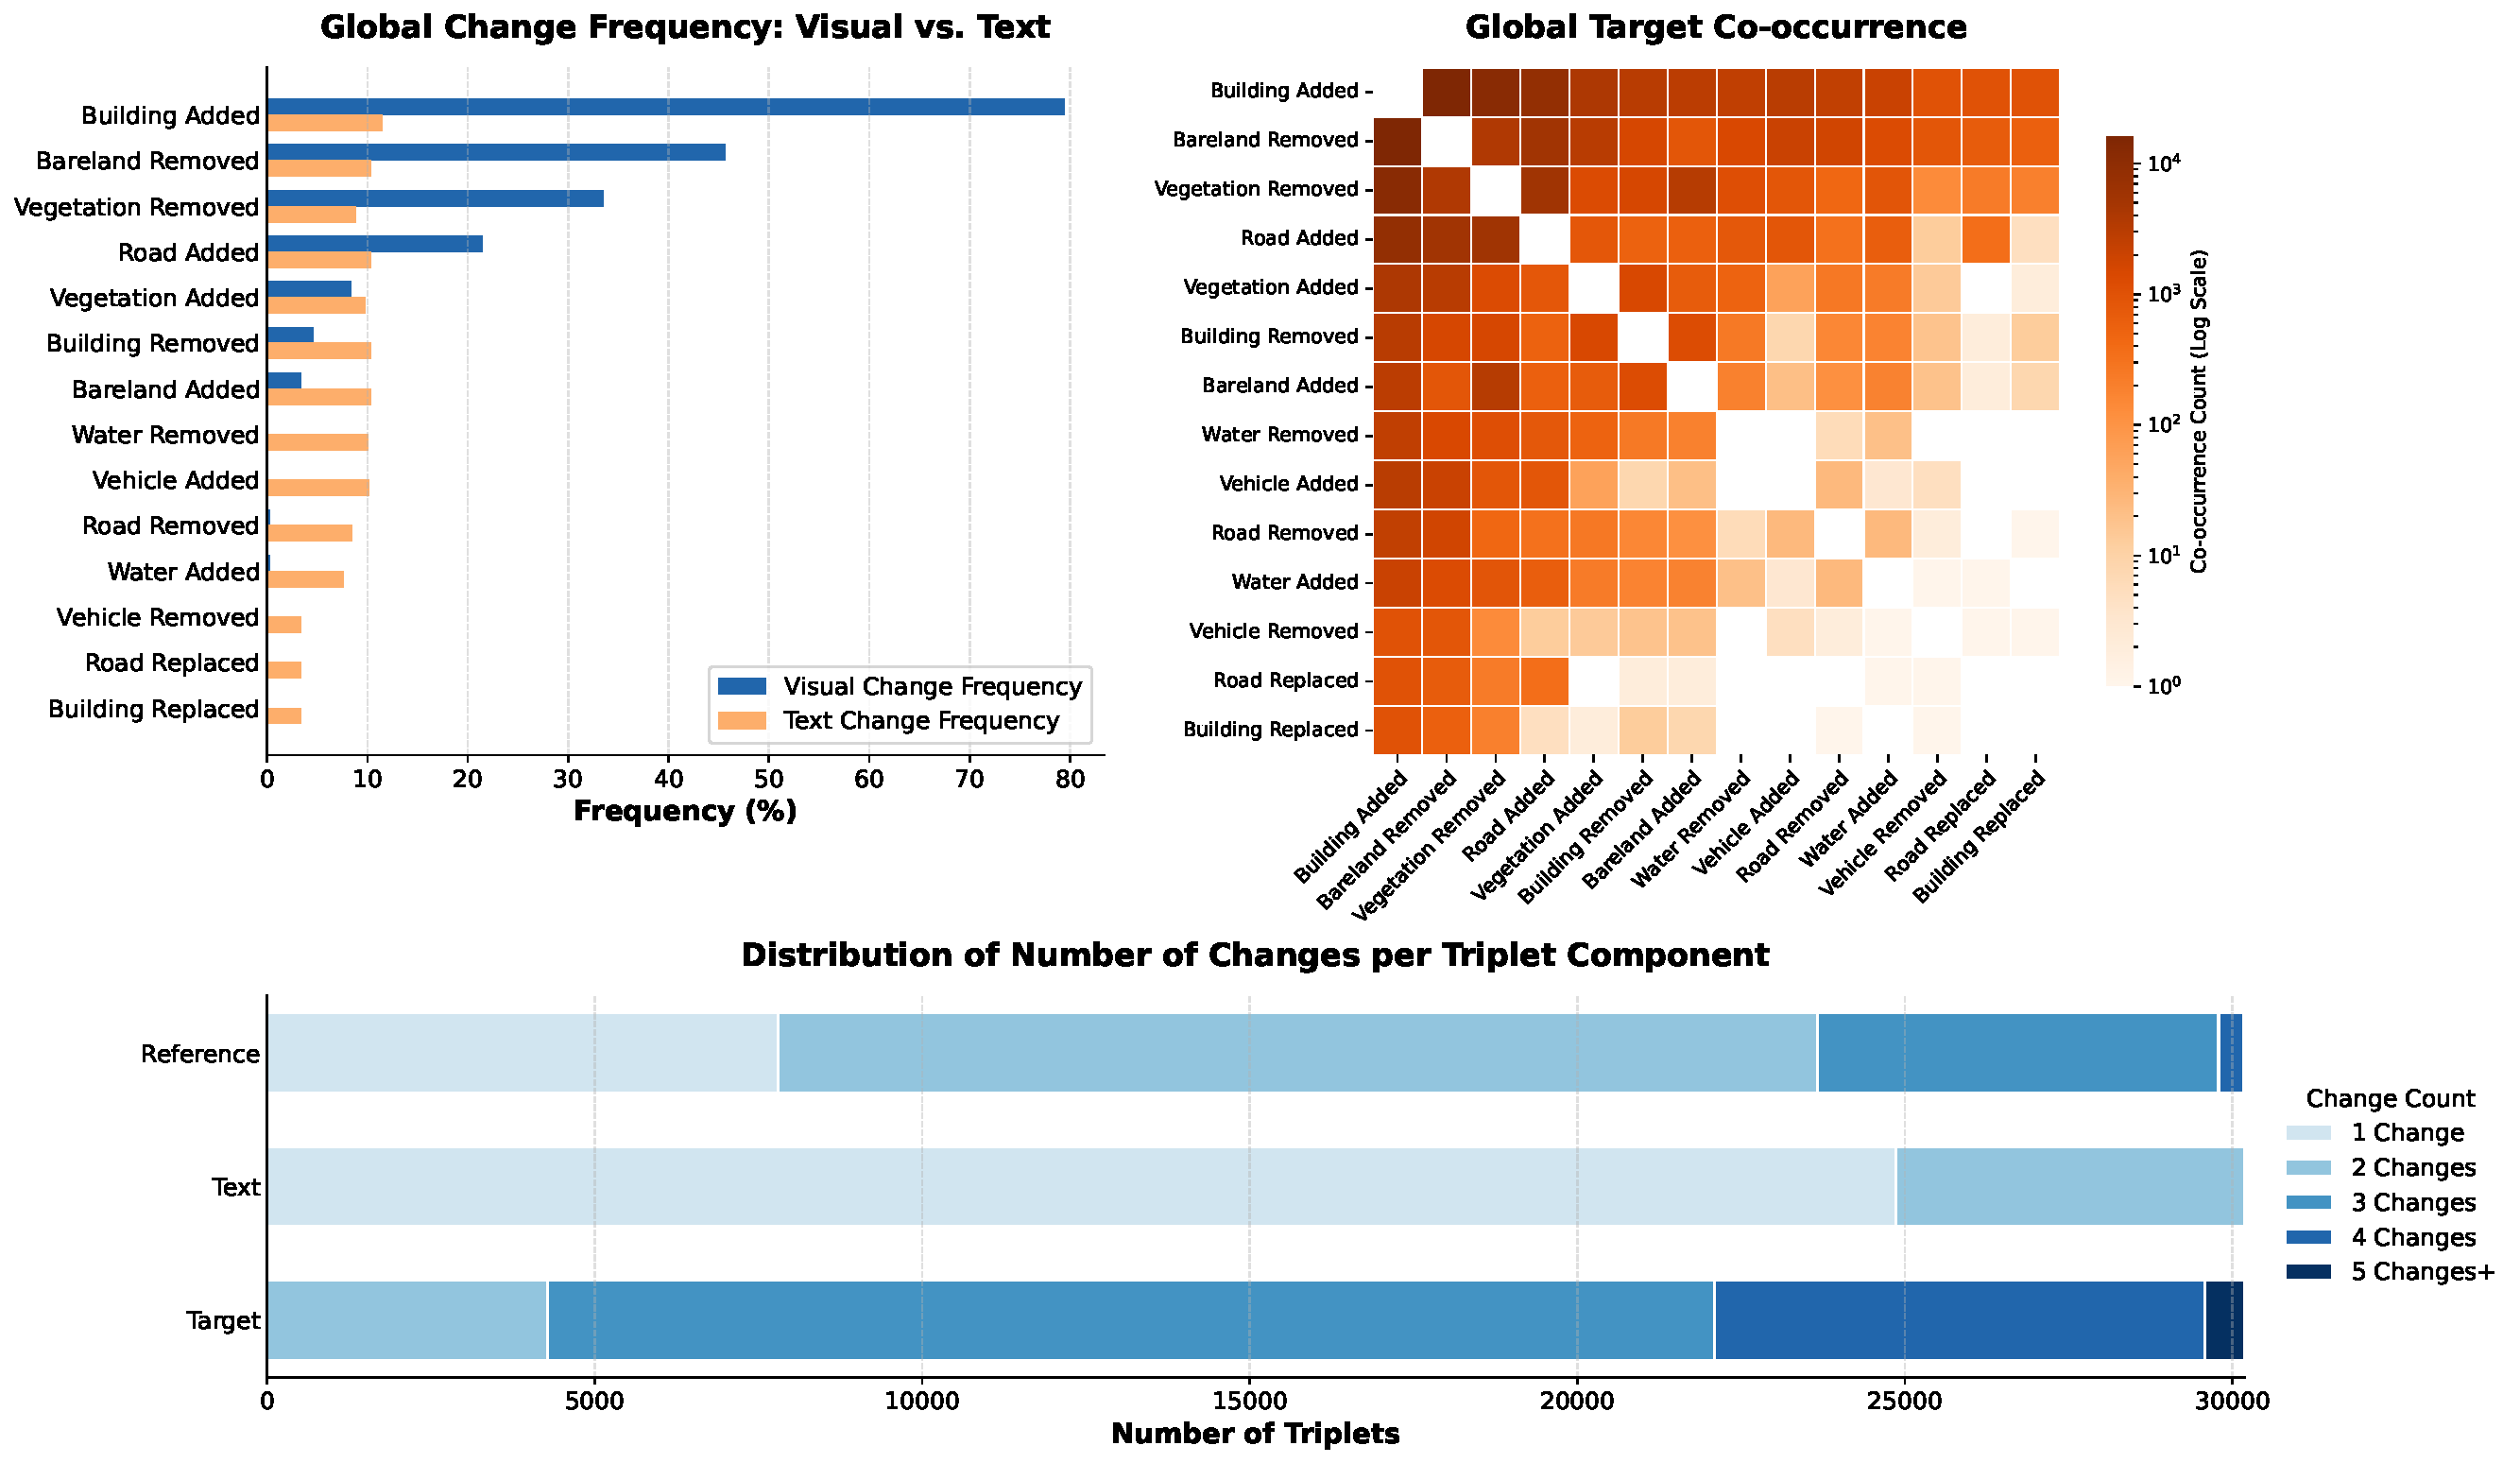
\includegraphics[width=\textwidth]{images/CTCR-RS/master_dataset_figure.pdf}
    \caption{CTCR-RS dataset statistics. \textbf{Top left}:
    visual (blue) vs.\ text (orange) change frequencies,
    demonstrating balanced text queries despite heavily
    unbalanced visual changes. \textbf{Top right}:
    log-scaled co-occurrence heatmap highlighting change
    correlations. \textbf{Bottom}: change counts per triplet
    component, visualizing the subset-superset task
    formulation.}
    \label{fig:chap6_stats}
\end{figure}
 
\textbf{Change frequency and bias mitigation.} The visual
change distribution $\mathcal{L}(\mathcal{I}_\text{ref})$
exhibits  a natural long-tail characteristic reflecting the
urban expansion dynamic dominant in LEVIR-CC and SECOND-CC:
Building Added and Bareland Removed
collectively dominate, while Replaced categories remain
rare, reflecting the infrequency of intra-class transitions
in the source datasets. To prevent the model from overfitting
to these visual changes, the text change synthesis ensures a
more balanced distribution of text queries
$\mathcal{C}_\text{text}$: less common change types are
more frequently selected as the textual modifier, resulting
in the orange distribution shown in
Figure~\ref{fig:chap6_stats} (top left).
 
\textbf{Change co-occurrence.} Building Added and Bareland
Removed co-occur strongly (Figure~\ref{fig:chap6_stats},
top right), reflecting the predominant urban expansion
pattern in the source datasets: new construction typically
occurs on previously bare land. This strong co-occurrence
is important to keep in mind when interpreting retrieval
performance: models that learn this correlation can partially
exploit it as a shortcut rather than performing genuine
compositional retrieval.
 
\textbf{Compositional complexity.} CTCR-RS moves beyond
single-attribute modifications. On average, each target
pair contains 3.2 simultaneous semantic changes. Notably,
over 85.81\% of the triplets require the model to compose
across three or more concurrent changes, a level of
complexity that challenges all baseline architectures as
shown in Section~\ref{sec:chap6_experiments}.
 
\textbf{One-to-many mapping.} Unlike standard CIR, the
CTCR-RS task is inherently one-to-many: multiple distinct
geographic locations can undergo identical land-use and
land-cover transitions. During training, the model
encounters an average of 39.1 positive targets per unique
change composition, a density that increases to 79.3 in the
test set, where 9,275 samples concentrate across only 117
unique compositions (compared to 298 in training). This
property has two important implications. First, it motivates
the Multiple Positives Enhanced NCE Loss described in
Section~\ref{sec:chap6_unictr_training}, which encourages
the model to learn generalized land-cover transition
representations rather than memorizing specific image
instances. Second, it means that standard retrieval metrics
computed against a single positive underestimate true
performance; the evaluation protocol described in
Section~\ref{sec:chap6_setup} accounts for all valid
positives.
 
\subsection{Compositional Triplet Generation}
\label{sec:chap6_triplets}
 
Retrieval triplets are constructed by exploiting the
subset-superset relationship between change label sets.
For every image pair $\mathcal{I}_\text{tar}$, we search
for potential reference pairs $\mathcal{I}_\text{ref}$
such that $\mathcal{L}(\mathcal{I}_\text{ref}) \subset
\mathcal{L}(\mathcal{I}_\text{tar})$. To ensure manageable
complexity while maintaining diversity, we restrict the
number of additional text changes
$n = |\mathcal{L}(\mathcal{I}_\text{tar}) \setminus
\mathcal{L}(\mathcal{I}_\text{ref})|$ to $n \in \{1, 2\}$.
 
Rather than using raw, inconsistent human captions as the
textual modifier, we generate the textual query
$\mathcal{C}_\text{text}$ using a standardized template:
\textit{``I want the same changes as in the reference pair,
plus [Extra Label(s)]''}. This ensures annotation precision
and consistency across the dataset, at the cost of
constraining the query to templated natural language rather
than free-form instructions, a limitation acknowledged
in Section~\ref{sec:chap6_conclusion}.
See Figure~\ref{fig:chap6_pipeline} for a visual overview of
the full dataset curation pipeline.

\subsection{Human Audit and Quality Validation}
\label{sec:chap6_audit}
 
To ensure the fidelity of the extracted change labels, we
conduct a rigorous manual audit on 600 stratified samples
randomly drawn from the dataset. For each sample, an expert
auditor compares the five raw human-authored captions, the
final normalized label set extracted by the LLM, and the
actual visual changes visible in the bi-temporal images.
 
\textbf{Overall results.} The LLM achieves an overall
extraction accuracy of 83.5\%, successfully and completely
mapping the free-form text to the correct visual reality in
501 of the 600 samples. Of the 99 failure cases (16.5\%),
78 errors (13.0\%) are true LLM hallucinations or extraction
misses where the model fails to properly synthesize the
captions, and 21 errors (3.5\%) stem from omissions or
errors in the original change captions themselves.
 
We provide examples of each outcome: LLM extraction
successes (Figure~\ref{fig:chap6_audit_success}), LLM
extraction misses (Figure~\ref{fig:chap6_audit_miss}),
and annotator errors and ambiguities
(Figure~\ref{fig:chap6_audit_error}).
 
\begin{figure}[ht]
    \centering
    % NOTE: insert Figure 1 from the supplementary here
    % (audit successes: two examples from LEVIR and SECOND
    % showing correct LLM extraction)
    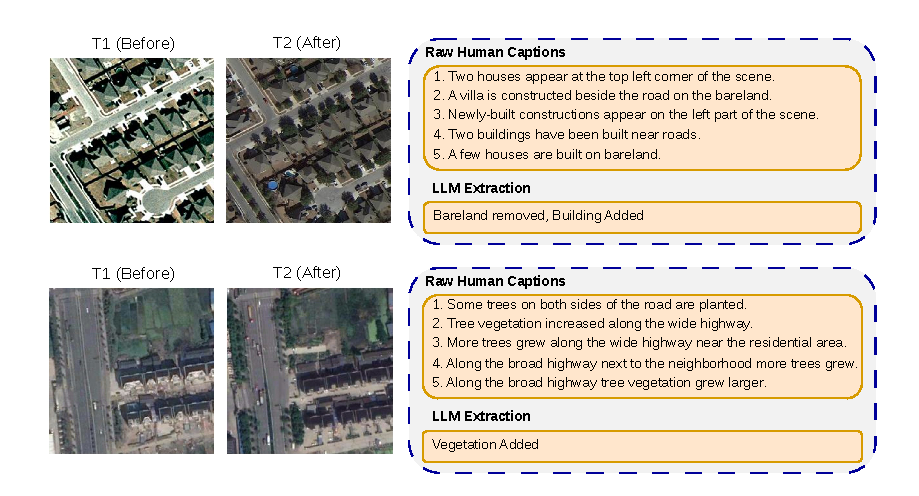
\includegraphics[width=0.85\textwidth]{images/CTCR-RS/supp-figure1-3.pdf}
    \caption{Audit successes: examples of correct LLM
    extraction across both source datasets. \textbf{Top
    (LEVIR-CC)}: the LLM correctly normalizes a building
    construction on bareland as Building Added + Bareland
    Removed. \textbf{Bottom (SECOND-CC)}: the LLM captures
    the distinct changes described by the annotators and maps
    them to the standard ontology.}
    \label{fig:chap6_audit_success}
\end{figure}
 
\begin{figure}[ht]
    \centering
    % NOTE: insert Figure 2 from the supplementary here
    % (LLM extraction misses: two examples where LLM
    % missed an explicitly stated label)
    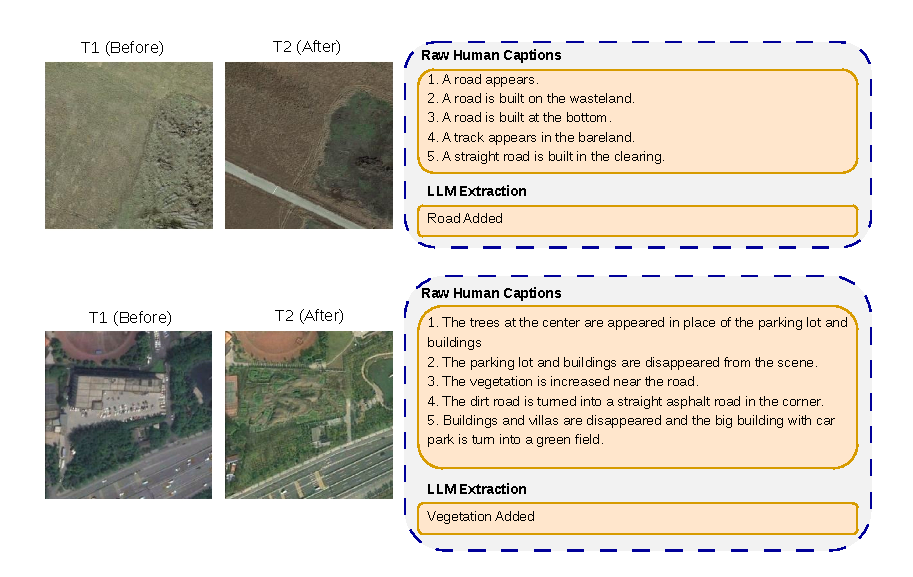
\includegraphics[width=0.85\textwidth]{images/CTCR-RS/supp_figure2.pdf}
    \caption{LLM extraction misses: examples where the
    pipeline failed to capture explicitly stated information.
    \textbf{Top (LEVIR-CC)}: Road Added is extracted but
    Bareland Removed is missed despite annotators mentioning
    the road was built on wasteland. \textbf{Bottom
    (SECOND-CC)}: Vegetation Added is extracted but Building
    Removed is dropped.}
    \label{fig:chap6_audit_miss}
\end{figure}
 
\begin{figure}[ht]
    \centering
    % NOTE: insert Figure 3 from the supplementary here
    % (annotator errors/ambiguity: temporal reversal, annotator
    % contradiction)
    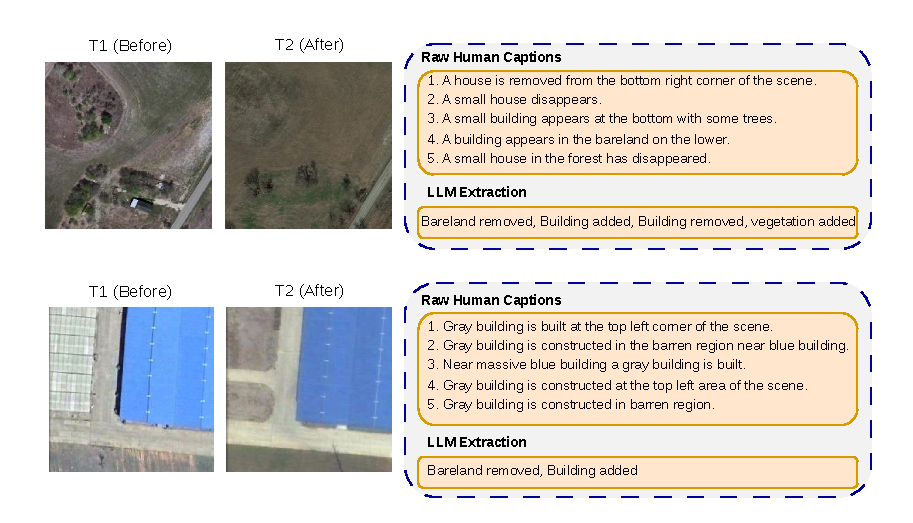
\includegraphics[width=0.85\textwidth]{images/CTCR-RS/supp-figure3.pdf}
    \caption{Errors originating from the original captions
    rather than the LLM pipeline. \textbf{Top (LEVIR-CC)}:
    annotator contradiction: some annotators describe a
    building as removed while others say it appears; the LLM
    extracts both. \textbf{Bottom (SECOND-CC)}: temporal
    reversal: the images show a demolition but the
    annotators describe it as construction.}
    \label{fig:chap6_audit_error}
\end{figure}
 
\textbf{LLM extraction misses (13.0\%).} These errors occur
when the model fails to capture all explicitly stated changes
from the captions. A common pattern is the omission of the
complementary removal label when annotators describe a
replacement (e.g., extracting Road Added but missing
Bareland Removed despite the annotators specifying the road
was built on wasteland). These errors are non-systematic and
do not concentrate on specific change types, suggesting they
are caused by the inherent difficulty of multi-label
extraction from ambiguous natural language rather than
systematic biases in the pipeline.
 
\textbf{Annotator errors and ambiguity (3.5\%).} A
qualitatively distinct error category arises not from the
LLM but from the source annotations themselves. Two
recurring patterns are particularly notable. First,
annotator contradiction: for the same bi-temporal pair,
some annotators describe a building as being demolished
while others describe a new building appearing, possibly
due to difficulty interpreting the temporal ordering of
before/after images. The LLM, faced with contradictory
instructions, extracts both changes. Second, temporal
reversal: annotators chronologically reverse the event,
describing a demolition as construction or vice versa. These errors
validate that 3.5\% of failures reflect genuine annotation
difficulty in the source datasets rather than deficiencies
in the curation pipeline.
 
\subsection{Dataset Splitting}
\label{sec:chap6_split}
 
The dataset is partitioned at the bi-temporal image pair
level \textit{prior} to triplet construction, yielding
11,660 / 9,244 / 9,275 triplets for training, validation,
and testing, corresponding to 3,768 / 925 / 945 unique
target image pairs respectively. Splitting at the image pair
level ensures that no bi-temporal image pair appears in
multiple splits, preventing information leakage through
shared visual content between training and evaluation
triplets.
 
% ============================================================
\section{Methodology}
\label{sec:chap6_method}
% ============================================================
 
To address the CTCR-RS task, we propose two complementary
architectures that progressively move from end-to-end latent
fusion to explicit semantic decomposition.
Figure~\ref{fig:chap6_arch} provides an overview of both.
 
\begin{figure}[ht]
    \centering
    % NOTE: insert Figure 4 from the main paper here
    % (architectural overview: UniCTCR left, StageCTCR right)
    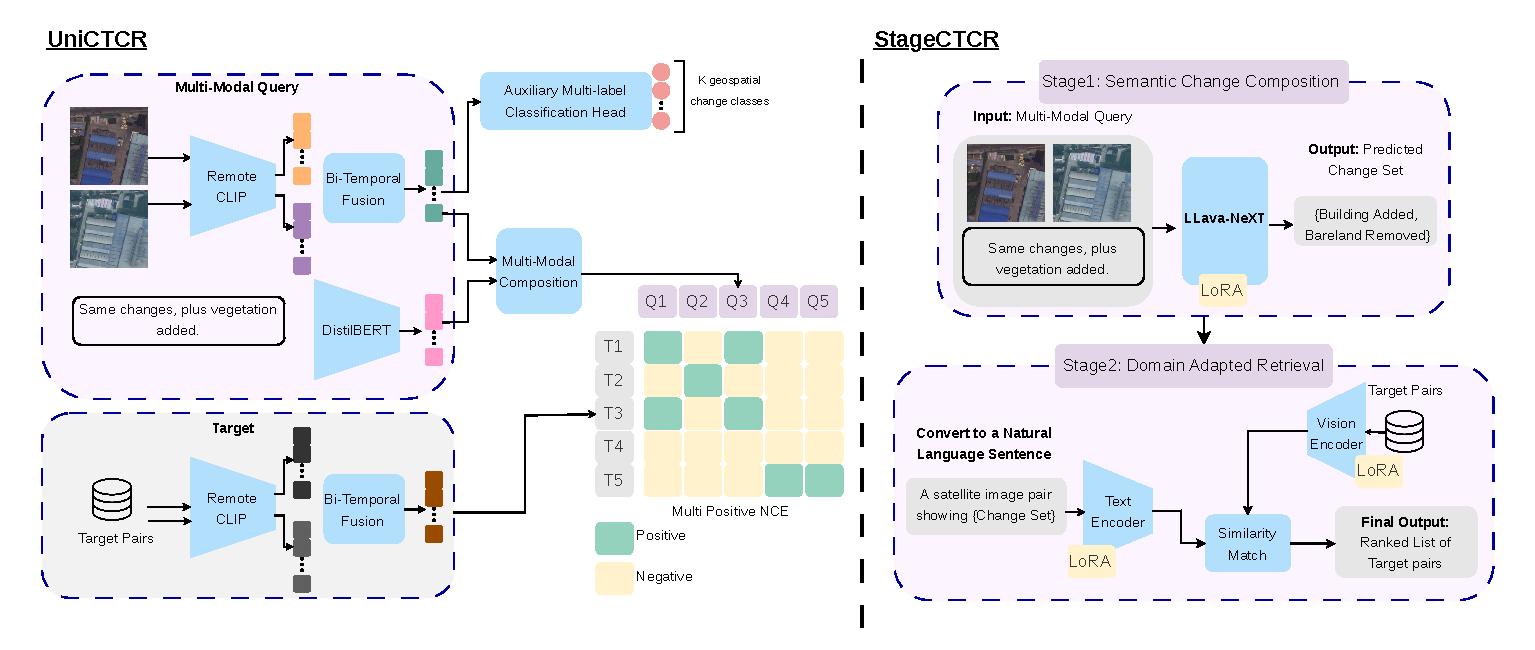
\includegraphics[width=0.85\textwidth]{images/CTCR-RS/figure-architecture-eccv.pdf}
    \caption{Architectural overview. \textbf{Left}: UniCTCR
    performs implicit multi-modal composition via bi-temporal
    feature fusion and Multi Positive NCE training.
    \textbf{Right}: StageCTCR decouples the task into
    VLM-based semantic composition (Stage~1, LLaVA-NeXT)
    and domain-adapted retrieval (Stage~2, RSICD-CLIP).}
    \label{fig:chap6_arch}
\end{figure}
 
\subsection{UniCTCR}
\label{sec:chap6_unictr}
 
UniCTCR is an end-to-end architecture that learns a joint
multi-modal change representation through dedicated fusion
and composition modules.
 
\subsubsection{Feature Extraction}
\label{sec:chap6_unictr_features}
 
Given a reference image pair $\mathcal{I} = (I_1, I_2)$
and a query text $\mathcal{C}_\text{text}$, we extract
unimodal representations as follows.
 
\textbf{Visual features.} For each image in the pair, we
use a pretrained RemoteCLIP~\cite{liu2024remoteclip} model
(ViT-B/32 backbone) to extract global embeddings $v_1,
v_2 \in \mathbb{R}^d$. RemoteCLIP is pretrained via
contrastive learning on large-scale RS image-text pairs,
providing representations that encode both fine-grained
spatial detail and high-level semantic content relevant to
land-cover categories.
 
\textbf{Textual features.} The query text
$\mathcal{C}_\text{text}$ is processed using pretrained
DistilBERT~\cite{sanh2019distilbert}, projecting the
\texttt{[CLS]} token to the joint embedding dimension $d$
to obtain the text representation $t \in \mathbb{R}^d$.
 
Both encoders are linearly projected into a shared $d = 512$
dimensional space and kept frozen during training, with all
trainable parameters concentrated in the fusion and
composition modules described below.
 
\subsubsection{Bi-Temporal Fusion}
\label{sec:chap6_unictr_fusion}
 
To aggregate the temporal information from $(v_1, v_2)$
into a unified semantic change representation
$v_\text{change}$, we evaluate three fusion strategies:
 
\textbf{Subtraction.} The most direct temporal modeling:
$v_\text{change} = v_2 - v_1$. This operation encodes the
direction of change in the embedding space, but assumes
that the difference vector is semantically meaningful, which
may not hold for complex multi-class transitions.
 
\textbf{Concatenation.} A learned linear projection of the
concatenated temporal features $[v_1; v_2]$. This allows
the model to learn a non-linear mapping from the joint
representation to a change embedding, without imposing the
strong assumption of the subtraction approach.
 
\textbf{Cross-Attention.} A bidirectional attention
mechanism over the $7 \times 7$ spatial patch embeddings
from both timesteps. Features are processed through a
3-layer transformer block (16 heads), mean-pooled, and
projected via a two-layer MLP, capturing complex
spatio-temporal interactions at the patch level. While
computationally more expensive, this approach can in
principle identify which spatial regions changed and reason
about the nature of the change, rather than operating on
global embeddings alone.
 
%Our ablation study (Table~\ref{tab:chap6_fusion}) shows
%that Concatenation achieves the highest global performance,
%marginally outperforming Subtraction and Cross-Attention.
%The narrow spread between the three strategies (less than
%4\% relative difference) suggests that the temporal fusion
%strategy is less critical than the downstream composition
%quality, which is the dominant bottleneck in this task.
 
\subsubsection{Multi-Modal Composition}
\label{sec:chap6_unictr_composition}
 
To fuse $v_\text{change}$ with the textual modification
$t$, we concatenate them into a joint representation
$h_\text{joint} = [v_\text{change}; t]$ and evaluate two
composition heads:
 
\textbf{MLP.} A standard two-layer MLP with ReLU
activation and dropout applied to $h_\text{joint}$ to
produce the final retrieval embedding $e_\text{ret}$.
 
\textbf{Gated Residual.} A dynamic pathway that modulates
the visual change based on the textual instruction. A
modulation gate $g$ (tanh activation) and a residual
correction $r$ are computed via parallel MLPs:
\begin{equation}
    e_\text{ret} = \text{Normalize}(v_\text{change}
    \odot g + r)
\end{equation}
This allows the model to selectively emphasize or suppress
aspects of the visual change representation based on what
the textual query requests.
%Despite its conceptual appeal,
%the standard MLP head substantially outperforms the Gated
%Residual in practice (0.23 vs. 0.12 R@1), suggesting that
%the dynamic modulation is harder to train with the
%available data.
 
\subsubsection{Target Encoding and Auxiliary Objective}
\label{sec:chap6_unictr_target}
 
Candidate target pairs $(I_1', I_2')$ in the retrieval
database are processed through the identical RemoteCLIP
encoder and bi-temporal fusion module to yield
$e_\text{target}$, enabling standard cosine similarity
matching against $e_\text{ret}$.
 
An auxiliary multi-label classification head is applied
directly to $v_\text{change}$ to predict the presence of
the $K$ land-cover change classes within the reference
pair. This two-layer MLP is trained with binary
cross-entropy and serves as an explicit regularizer: it
forces the bi-temporal fusion module to produce
semantically meaningful change representations before the
composition module operates on them.
 
\subsubsection{Training Objectives}
\label{sec:chap6_unictr_training}
 
To address the one-to-many mapping property of the
CTCR-RS task, UniCTCR is trained with a composite
objective. Let $\mathcal{P}(i)$ be the set of all valid
positive targets for query $i$, and $S_{ij} =
(e_\text{ret}^{(i)} \cdot e_\text{target}^{(j)}) / \tau$
be the scaled cosine similarity with temperature $\tau$.
The Multiple Positives Enhanced NCE loss aggregates
probability mass over all valid positives:
\begin{equation}
    \mathcal{L}_\text{nce}^{(i)} = -\log
    \frac{\sum_{p \in \mathcal{P}(i)} \exp(S_{ip})}
    {\sum_{j \in \mathcal{A}(i)} \exp(S_{ij})}
    \label{eq:mpnce}
\end{equation}
where $\mathcal{A}(i)$ represents all samples in the
batch. This is coupled with a similarity regularization
term $\mathcal{L}_\text{sim}^{(i)}$ that directly maximizes
the mean unscaled cosine similarity of all positive pairs.
The full training objective is:
\begin{equation}
    \mathcal{L}_\text{total} = \frac{1}{N}
    \sum_{i=1}^N \left(
    \mathcal{L}_\text{nce}^{(i)} +
    \alpha \mathcal{L}_\text{sim}^{(i)}
    \right) + \lambda \mathcal{L}_\text{aux}
    \label{eq:unictr_loss}
\end{equation}
UniCTCR is trained with AdamW, learning rate $5 \times
10^{-4}$, weight decay 0.01, batch size 512, dropout 0.2,
for 40 epochs.
 
\subsection{StageCTCR}
\label{sec:chap6_stagectcr}
 
Motivated by the oracle analysis of UniCTCR (see Table \ref{tab:chap6_fusion}), which reveals
that the primary bottleneck lies in multi-modal composition
rather than retrieval, StageCTCR explicitly decomposes the
problem into two independent stages: semantic change
composition followed by domain-adapted retrieval. This
eliminates the need for learned latent fusion, replacing it
with the explicit reasoning capabilities of a pretrained
VLM.
 
\subsubsection{Stage 1: Semantic Change Composition}
\label{sec:chap6_stage1}
 
The first stage employs LLaVA-NeXT~\cite{liu2024llavanext}
as a semantic change composition engine. Given the textual
query structure ``\textit{I want the same changes as the
reference pair, plus $\mathcal{C}_\text{text}$}'', the VLM
must visually deduce the changes present in
$\mathcal{I}_\text{ref}$ and integrate them with
$\mathcal{C}_\text{text}$ to predict the full target change
set $\mathcal{L}(\mathcal{I}_\text{tar})$.
 
To provide the VLM with a single image input, the reference
pair is spatially concatenated into a unified composite
image $I_\text{comp} \in \mathbb{R}^{H \times 2W \times 3}$,
with ``BEFORE'' and ``AFTER'' text markers digitally
overlaid to provide explicit temporal grounding. LLaVA-NeXT
is fine-tuned via LoRA to output a strict, comma-separated
string from the change ontology.
 
LoRA is applied to all linear layers within the language
model backbone (attention and feed-forward projections),
while the vision tower, multimodal projector, and language
modeling head are kept frozen. Configuration: rank $r = 64$,
scaling factor $\alpha = 128$, dropout 0.05, fine-tuned for
3 epochs at learning rate $2 \times 10^{-4}$ with
AdamW~\cite{adamw}.
 
\subsubsection{Stage 2: Domain-Adapted Retrieval}
\label{sec:chap6_stage2}
 
The second stage is a dedicated retrieval backbone. A CLIP
model pretrained on RSICD~\cite{lu2017exploring} is
fine-tuned via LoRA to project both modalities into a
shared retrieval space. The structured target list
$\mathcal{L}(\mathcal{I}_\text{tar})$ predicted by Stage~1
is converted into a natural language prompt (e.g., ``\textit{A
satellite image pair showing [change list]}''), which the
CLIP text encoder processes to yield the text embedding
$e_\text{text} \in \mathbb{R}^d$. Symmetrically, candidate
target pairs are horizontally concatenated,
letterbox-padded to $224 \times 224$, and processed by the
CLIP vision encoder to yield $e_\text{target} \in
\mathbb{R}^d$.
 
LoRA is applied to the projection layers of both CLIP
encoders (configuration: $r = 16$, $\alpha = 32$, dropout
0.05), and both encoders are fine-tuned jointly using a
symmetric InfoNCE loss for 5 epochs at learning rate
$10^{-4}$ with AdamW.
 
% ============================================================
\section{Experimental Study}
\label{sec:chap6_experiments}
% ============================================================
 
\subsection{Experimental Setup}
\label{sec:chap6_setup}
 
\textbf{Evaluation metrics.} We report standard retrieval
metrics: Recall at $k$ (R@1, R@5, R@10, R@20), Median
Rank (MedR, lower is better), and Mean Average Precision
at 5 (mAP@5). All metrics are computed over the full test
set. Since the task is one-to-many, a retrieved pair is
considered correct if it belongs to the set of all valid
positives for the query composition.
 
\textbf{Complexity stratification.} In addition to the
global test set, results are reported across two orthogonal
complexity dimensions. \textit{Text Query complexity} refers
to the number of additional changes specified in
$\mathcal{C}_\text{text}$ (1 or 2). \textit{Visual Query
complexity} refers to the number of changes present in the
reference image pair $\mathcal{I}_\text{ref}$ (1, 2, or
$>$2). The two stratifications are overlapping and not
mutually exclusive, allowing independent assessment of
textual composition difficulty versus visual change
disentanglement difficulty.
 
\textbf{Oracle baselines.} Two oracle baselines establish
upper bounds. The \textit{Text-Only Oracle} for UniCTCR
replaces the composed query with the full ground-truth
target description, measuring the upper bound of
text-to-visual retrieval within the UniCTCR architecture.
The \textit{GT+CLIP Upper Bound} applies the same oracle
strategy within StageCTCR's retrieval stage, replacing
LLaVA-NeXT predictions with ground-truth labels. Neither
oracle is a realistic inference-time setting; both serve
to isolate retrieval difficulty from composition difficulty.
 
\textbf{Baselines.} We compare against SEARLE~\cite{baldrati2023zero}
(zero-shot CIR using only the post-change image $I_2$) and
CoVR~\cite{ventura2024covr} (composed video retrieval,
adapted by stacking $I_1$ and $I_2$ spatially),
zero-shot and after fine-tuning on CTCR-RS.
 
\subsection{UniCTCR: Ablation of Fusion Strategies and
Composition Heads}
\label{sec:chap6_unictr_results}
\textbf{Fusion strategy.} Concatenation achieves the
highest global performance (R@1 = 0.24, mAP@5 = 0.66),
marginally outperforming Subtraction (0.23 R@1) and
Cross-Attention (0.22 R@1). The narrow spread between the
three strategies (approximately 4\% relative difference)
suggests that the temporal fusion strategy is less critical
than the downstream composition quality. Cross-Attention
provides better results at high visual complexity ($>$2
changes), likely because patch-level spatial attention
helps disentangle overlapping changes, but Concatenation
is more robust across the majority of the dataset. This
indicates that simpler fusion adequately captures
multi-modal relationships for global feature-level
operations.
 
\textbf{Composition head.} The standard MLP head
substantially outperforms the Gated Residual fusion
(0.23 vs. 0.12 R@1 globally), with the Gated Residual
struggling particularly on simpler single-change queries
where its dynamic gating mechanism appears to overfit.
 
\textbf{Oracle analysis.} The Text-Only Oracle achieves
R@1 = 0.30, exceeding the best UniCTCR configuration.
This establishes an important reference point: the
performance gap between UniCTCR (0.24) and the oracle
(0.30) is attributable entirely to the composition step,
confirming that identifying and fusing the composed
visual-textual change is the primary bottleneck. The
oracle also underperforms on top-rank metrics for single
visual changes (0.31 vs. 0.42 R@1), where the visual
reference provides stronger signal than a text description.
 
\begin{table}[htb]
\centering
\footnotesize
\caption{Ablation of bi-temporal fusion strategies and
composition heads for UniCTCR. \textbf{Global} reports
results on the full test set; subsequent rows stratify by
text and visual complexity. Best non-oracle R@1 result per
complexity level in \textbf{bold}.}
\label{tab:chap6_fusion}
\resizebox{0.85 \textwidth}{!}{
\begin{tabularx}{\textwidth}{ll
    >{\centering\arraybackslash}X
    >{\centering\arraybackslash}X
    >{\centering\arraybackslash}X
    >{\centering\arraybackslash}X
    >{\centering\arraybackslash}X
    >{\centering\arraybackslash}X}

\toprule
\textbf{Method} & \textbf{Complexity}
& R@1 & R@5 & R@10 & R@20 & MedR$\downarrow$ & mAP@5 \\
\midrule
\multirow{6}{*}{MLP + Concat.}
& Global           & \textbf{0.24} & 0.47 & 0.62 & 0.72 & 6  & 0.66 \\
& 1 Text Change    & \textbf{0.22} & 0.45 & 0.61 & 0.70 & 7  & 0.66 \\
& 2 Text Changes   & 0.39 & 0.68 & 0.77 & 0.85 & 2  & 0.70 \\
& 1 Visual Change  & \textbf{0.42} & 0.78 & 0.89 & 0.94 & 2  & 0.67 \\
& 2 Visual Changes & 0.24 & 0.49 & 0.64 & 0.77 & 5  & 0.66 \\
& $>$2 Visual      & 0.07 & 0.16 & 0.33 & 0.40 & 36 & 0.63 \\
\midrule
\multirow{6}{*}{MLP + CrossAttn.}
& Global           & 0.22 & 0.47 & 0.59 & 0.70 & 6  & 0.63 \\
& 1 Text Change    & 0.20 & 0.45 & 0.57 & 0.69 & 7  & 0.61 \\
& 2 Text Changes   & \textbf{0.42} & 0.68 & 0.77 & 0.82 & 2  & 0.74 \\
& 1 Visual Change  & 0.30 & 0.73 & 0.86 & 0.93 & 3  & 0.59 \\
& 2 Visual Changes & 0.24 & 0.47 & 0.59 & 0.72 & 7  & 0.67 \\
& $>$2 Visual      & \textbf{0.09} & 0.27 & 0.35 & 0.47 & 23 & 0.54 \\
\midrule
\multirow{6}{*}{MLP + Sub.}
& Global           & 0.23 & 0.49 & 0.58 & 0.70 & 6  & 0.62 \\
& 1 Text Change    & 0.21 & 0.48 & 0.57 & 0.70 & 7  & 0.60 \\
& 2 Text Changes   & 0.38 & 0.64 & 0.75 & 0.84 & 3  & 0.71 \\
& 1 Visual Change  & 0.37 & 0.78 & 0.87 & 0.94 & 2  & 0.63 \\
& 2 Visual Changes & \textbf{0.25} & 0.50 & 0.62 & 0.76 & 5  & 0.64 \\
& $>$2 Visual      & 0.04 & 0.22 & 0.25 & 0.37 & 41 & 0.39 \\
\midrule
\multirow{6}{*}{GRes + Sub.}
& Global           & 0.12 & 0.39 & 0.51 & 0.69 & 10 & 0.55 \\
& 1 Text Change    & 0.11 & 0.36 & 0.49 & 0.67 & 11 & 0.54 \\
& 2 Text Changes   & 0.21 & 0.66 & 0.74 & 0.83 & 3  & 0.57 \\
& 1 Visual Change  & 0.28 & 0.67 & 0.75 & 0.92 & 3  & 0.64 \\
& 2 Visual Changes & 0.11 & 0.41 & 0.55 & 0.74 & 9  & 0.51 \\
& $>$2 Visual      & 0.00 & 0.11 & 0.22 & 0.38 & 38 & 0.37 \\
\midrule
\multirow{6}{*}{Text-Oracle}
& Global           & 0.30 & 0.50 & 0.69 & 0.81 & 6  & 0.70 \\
& 1 Text Change    & 0.29 & 0.48 & 0.67 & 0.80 & 6  & 0.68 \\
& 2 Text Changes   & 0.55 & 0.66 & 0.77 & 0.87 & 1  & 0.88 \\
& 1 Visual Change  & 0.31 & 0.47 & 0.79 & 0.97 & 6  & 0.74 \\
& 2 Visual Changes & 0.36 & 0.59 & 0.81 & 0.92 & 4  & 0.68 \\
& $>$2 Visual      & 0.18 & 0.26 & 0.32 & 0.42 & 29 & 0.79 \\
\bottomrule
\end{tabularx}}
\end{table}



\subsection{StageCTCR: Decomposed Retrieval}
\label{sec:chap6_stagectcr_results}
\begin{table}[htb]
\centering
\footnotesize
\caption{StageCTCR performance and error analysis across
complexity levels. \textbf{GT+CLIP} replaces LLaVA-NeXT
predictions with ground-truth labels to isolate Stage~2.}
\label{tab:chap6_stagectcr}
\begin{tabularx}{\textwidth}{ll
    >{\centering\arraybackslash}X
    >{\centering\arraybackslash}X
    >{\centering\arraybackslash}X
    >{\centering\arraybackslash}X
    >{\centering\arraybackslash}X
    >{\centering\arraybackslash}X}
\toprule
\textbf{Method} & \textbf{Complexity}
& R@1 & R@5 & R@10 & R@20 & MedR$\downarrow$ & mAP@5 \\
\midrule
\multirow{6}{*}{\shortstack{StageCTCR\\(LLaVA-NeXT + CLIP)}}
& Global           & 0.33 & 0.49 & 0.62 & 0.72 & 6  & 0.77 \\
& 1 Text Change    & 0.31 & 0.45 & 0.53 & 0.70 & 8  & 0.75 \\
& 2 Text Changes   & 0.63 & 0.73 & 0.80 & 0.86 & 1  & 0.85 \\
& 1 Visual Change  & 0.57 & 0.74 & 0.80 & 0.87 & 1  & 0.80 \\
& 2 Visual Changes & 0.34 & 0.48 & 0.58 & 0.77 & 8  & 0.78 \\
& $>$2 Visual      & 0.12 & 0.25 & 0.28 & 0.44 & 49 & 0.64 \\
\midrule
\multirow{6}{*}{\shortstack{Upper Bound\\(GT + CLIP)}}
& Global           & 0.41 & 0.54 & 0.63 & 0.73 & 3  & 0.81 \\
& 1 Text Change    & 0.38 & 0.51 & 0.61 & 0.71 & 4  & 0.80 \\
& 2 Text Changes   & 0.69 & 0.79 & 0.84 & 0.89 & 1  & 0.86 \\
& 1 Visual Change  & 0.60 & 0.85 & 0.87 & 0.88 & 1  & 0.78 \\
& 2 Visual Changes & 0.42 & 0.52 & 0.68 & 0.81 & 3  & 0.82\\
& $>$2 Visual      & 0.22 & 0.30 & 0.31 & 0.40 & 49 & 0.80\\
\bottomrule
\end{tabularx}
\end{table}
 
\textbf{Overall performance.} StageCTCR achieves 0.33 R@1
globally, a +9\% absolute improvement over the best
UniCTCR configuration, and 0.77 mAP@5. Crucially,
StageCTCR surpasses UniCTCR's Text-Only Oracle (0.30 R@1)
at inference time, demonstrating two critical points: first,
explicit semantic composition provides a stronger inductive
bias than implicit latent fusion; second, CLIP's pretrained
cross-modal alignment, adapted via LoRA for the RS domain,
is superior to the alignment learned by UniCTCR's projection
modules.
 
\textbf{Stage 1 evaluation.} LLaVA-NeXT independently
achieves Precision: 0.860, Recall: 0.882, F1: 0.871 on
the test set. This validates its role as a reliable
semantic change composer. However, due to strict
multi-label matching, minor prediction errors still cascade
into retrieval penalties: a single missed label in the
predicted change set directs Stage~2 retrieval toward the
wrong semantic cluster.
 
\textbf{Stage 1 vs. Stage 2 decomposition.} Replacing
LLaVA-NeXT predictions with ground-truth labels (GT+CLIP,
Table~\ref{tab:chap6_stagectcr}) yields R@1 = 0.41, an 8\% gap that isolates Stage~1 errors. This
gap confirms that semantic composition is still a limiting
factor even for a strong VLM. Comparing GT+CLIP (0.41) to
UniCTCR's Text-Only Oracle (0.30) shows that CLIP's
pretrained alignment provides a 37\% relative improvement
over UniCTCR's learned projection, even when both use
text-only inputs, confirming that the retrieval stage gains
are attributable to the CLIP backbone, not just the
explicitly structured input format.
 
\subsection{Comparison with Existing Methods}
\label{sec:chap6_comparison}
 
\begin{table}[htb]
\centering
\footnotesize
\caption{Summary comparison of existing methods, proposed
approaches, and oracle upper bounds.}
\label{tab:chap6_comparison}
\begin{tabularx}{\textwidth}{l
    >{\centering\arraybackslash}X
    >{\centering\arraybackslash}X
    >{\centering\arraybackslash}X
    >{\centering\arraybackslash}X
    >{\centering\arraybackslash}X}
\toprule
\textbf{Method}
& R@1 & R@5 & R@10 & MedR$\downarrow$ & mAP@5 \\
\midrule
SEARLE~\cite{baldrati2023zero} (Zero-Shot, $I_2$ only)
& 0.07 & 0.21 & 0.36 & 18 & 0.07 \\
CoVR~\cite{ventura2024covr} (Zero-Shot, stacked frames)
& 0.07 & 0.23 & 0.36 & 18 & 0.53 \\
CoVR~\cite{ventura2024covr} (Fine-Tuned, stacked frames)
& 0.11 & 0.37 & 0.52 & 10 & 0.54 \\
UniCTCR (Concat+MLP, RemoteCLIP)
& 0.24 & 0.47 & 0.62 & 6  & 0.66 \\
UniCTCR (Concat+MLP, CLIP ViT-L/14)
& 0.21 & 0.48 & 0.61 & 6  & 0.62 \\
Text-Only Oracle
& 0.30 & 0.50 & 0.69 & 6  & 0.70 \\
\textbf{StageCTCR (LLaVA-NeXT + CLIP)}
& 0.33 & 0.49 & 0.62 & 6  & 0.77 \\
Upper Bound (GT + CLIP)
& 0.41 & 0.54 & 0.63 & 3  & 0.81 \\
\bottomrule
\end{tabularx}
\end{table}
 
\textbf{CIR baseline (SEARLE).} Given only the
post-change image $I_2$ due to the single-image constraint,
this zero-shot model achieves just 0.07 R@1, confirming
that capturing the temporal change is strictly necessary
to contextualize text queries in this setting. A model
that ignores the reference pair's visual change cannot
compose a meaningful query.
 
\textbf{CoVR baseline.} Adapting CoVR by spatially stacking
$I_1$ and $I_2$ yields 0.07 R@1 zero-shot and 0.11 R@1
after fine-tuning. Despite conceptually similar temporal
structure (two frames), the CoVR architecture fails to
model discrete land-cover changes, confirming that
the paradigm transfer from continuous video to bi-temporal
satellite imagery is structurally invalid.
 
\textbf{Encoder ablation.} To verify that StageCTCR's gains
stem from its staged decomposition rather than a stronger
encoder, we replace UniCTCR's RemoteCLIP backbone with
CLIP ViT-L/14, keeping all other components identical.
Despite using a larger and generally stronger encoder,
UniCTCR performs worse (0.21 vs. 0.24 R@1), confirming
that the performance gap between UniCTCR and StageCTCR is
architectural rather than encoder-driven.
 
\subsection{Complexity Analysis}
\label{sec:chap6_complexity}
 
\textbf{Text Query Complexity.} Performance improves with
more text changes: StageCTCR achieves 0.31 R@1 for
1-change queries but 0.63 R@1 for 2-change queries. This
counterintuitive result reflects semantic distinctiveness:
2-change queries contain highly discriminative label pairs
(e.g., ``Bareland Removed'' + ``Road Added''), while
1-change queries include inherently ambiguous labels
(e.g., ``Water Removed'' achieves just 0.014 R@1). A
single common change type does not uniquely identify a
target composition, whereas two concurrent changes
substantially narrow the retrieval space.
 
\textbf{Visual Complexity (Reference Pair).} Performance
degrades monotonically: StageCTCR achieves 0.57 R@1 for
reference pairs with 1 visual change but only 0.12 R@1
for reference pairs with $>$2 changes. Critically, even
the GT+CLIP upper bound struggles at $>$2 visual changes
(0.22 R@1, MedR = 49). This indicates that the performance
drop can be attributed to the target encoding process:
when four or more concurrent changes co-occur in a target
pair, global vision encoders produce entangled embeddings
in which individual change signatures are no longer
discriminable. This is a fundamental limitation of
single-vector global representations and motivates future
work on patch-level or change-specific encoding strategies.
 
\subsection{Qualitative Results}
\label{sec:chap6_qualitative}
 
\begin{figure}[ht]
    \centering
    % NOTE: insert Figure 4 from the supplementary here
    % (qualitative retrieval successes: 2 visual changes + 1
    % text change, StageCTCR correctly retrieves, UniCTCR
    % struggles)
    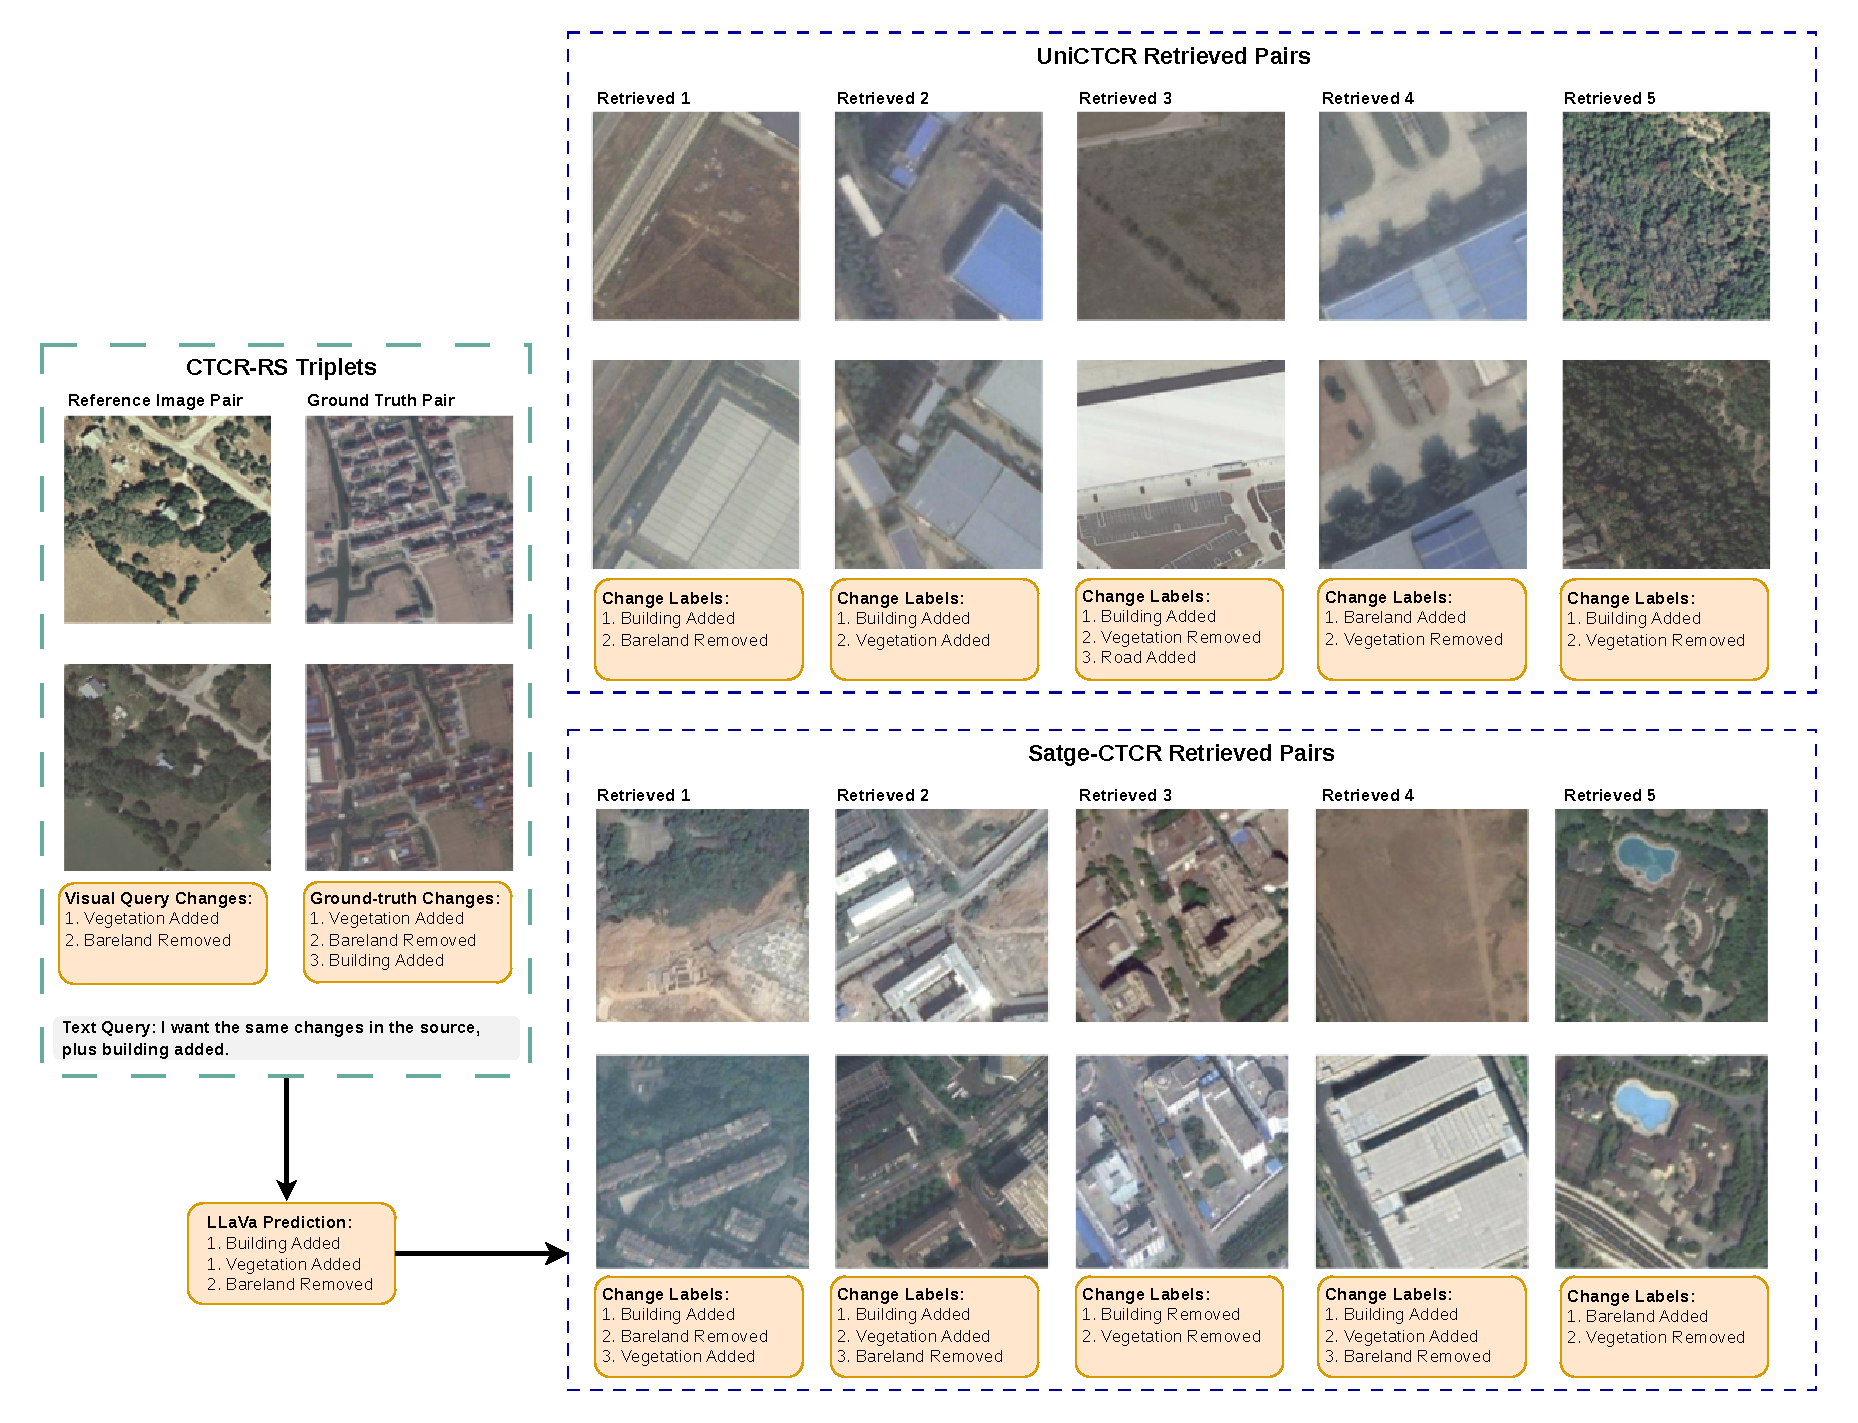
\includegraphics[width=0.85\textwidth]{images/CTCR-RS/supp-figure4.pdf}
    \caption{Qualitative retrieval successes. Given a
    reference pair with 2 visual changes (Vegetation Added,
    Bareland Removed) and a text query (Building Added),
    StageCTCR retrieves 3 correct pairs in the top 5 (ranks
    1, 2, 4), while UniCTCR retrieves pairs that omit
    specific changes. LLaVA-NeXT correctly predicts the full
    change set.}
    \label{fig:chap6_qual_success}
\end{figure}
 
\begin{figure}[ht]
    \centering
    % NOTE: insert Figure 5 from the supplementary here
    % (qualitative retrieval with LLaVA failure: 3 visual
    % changes + 1 text, LLaVA misses Vegetation Removed)
    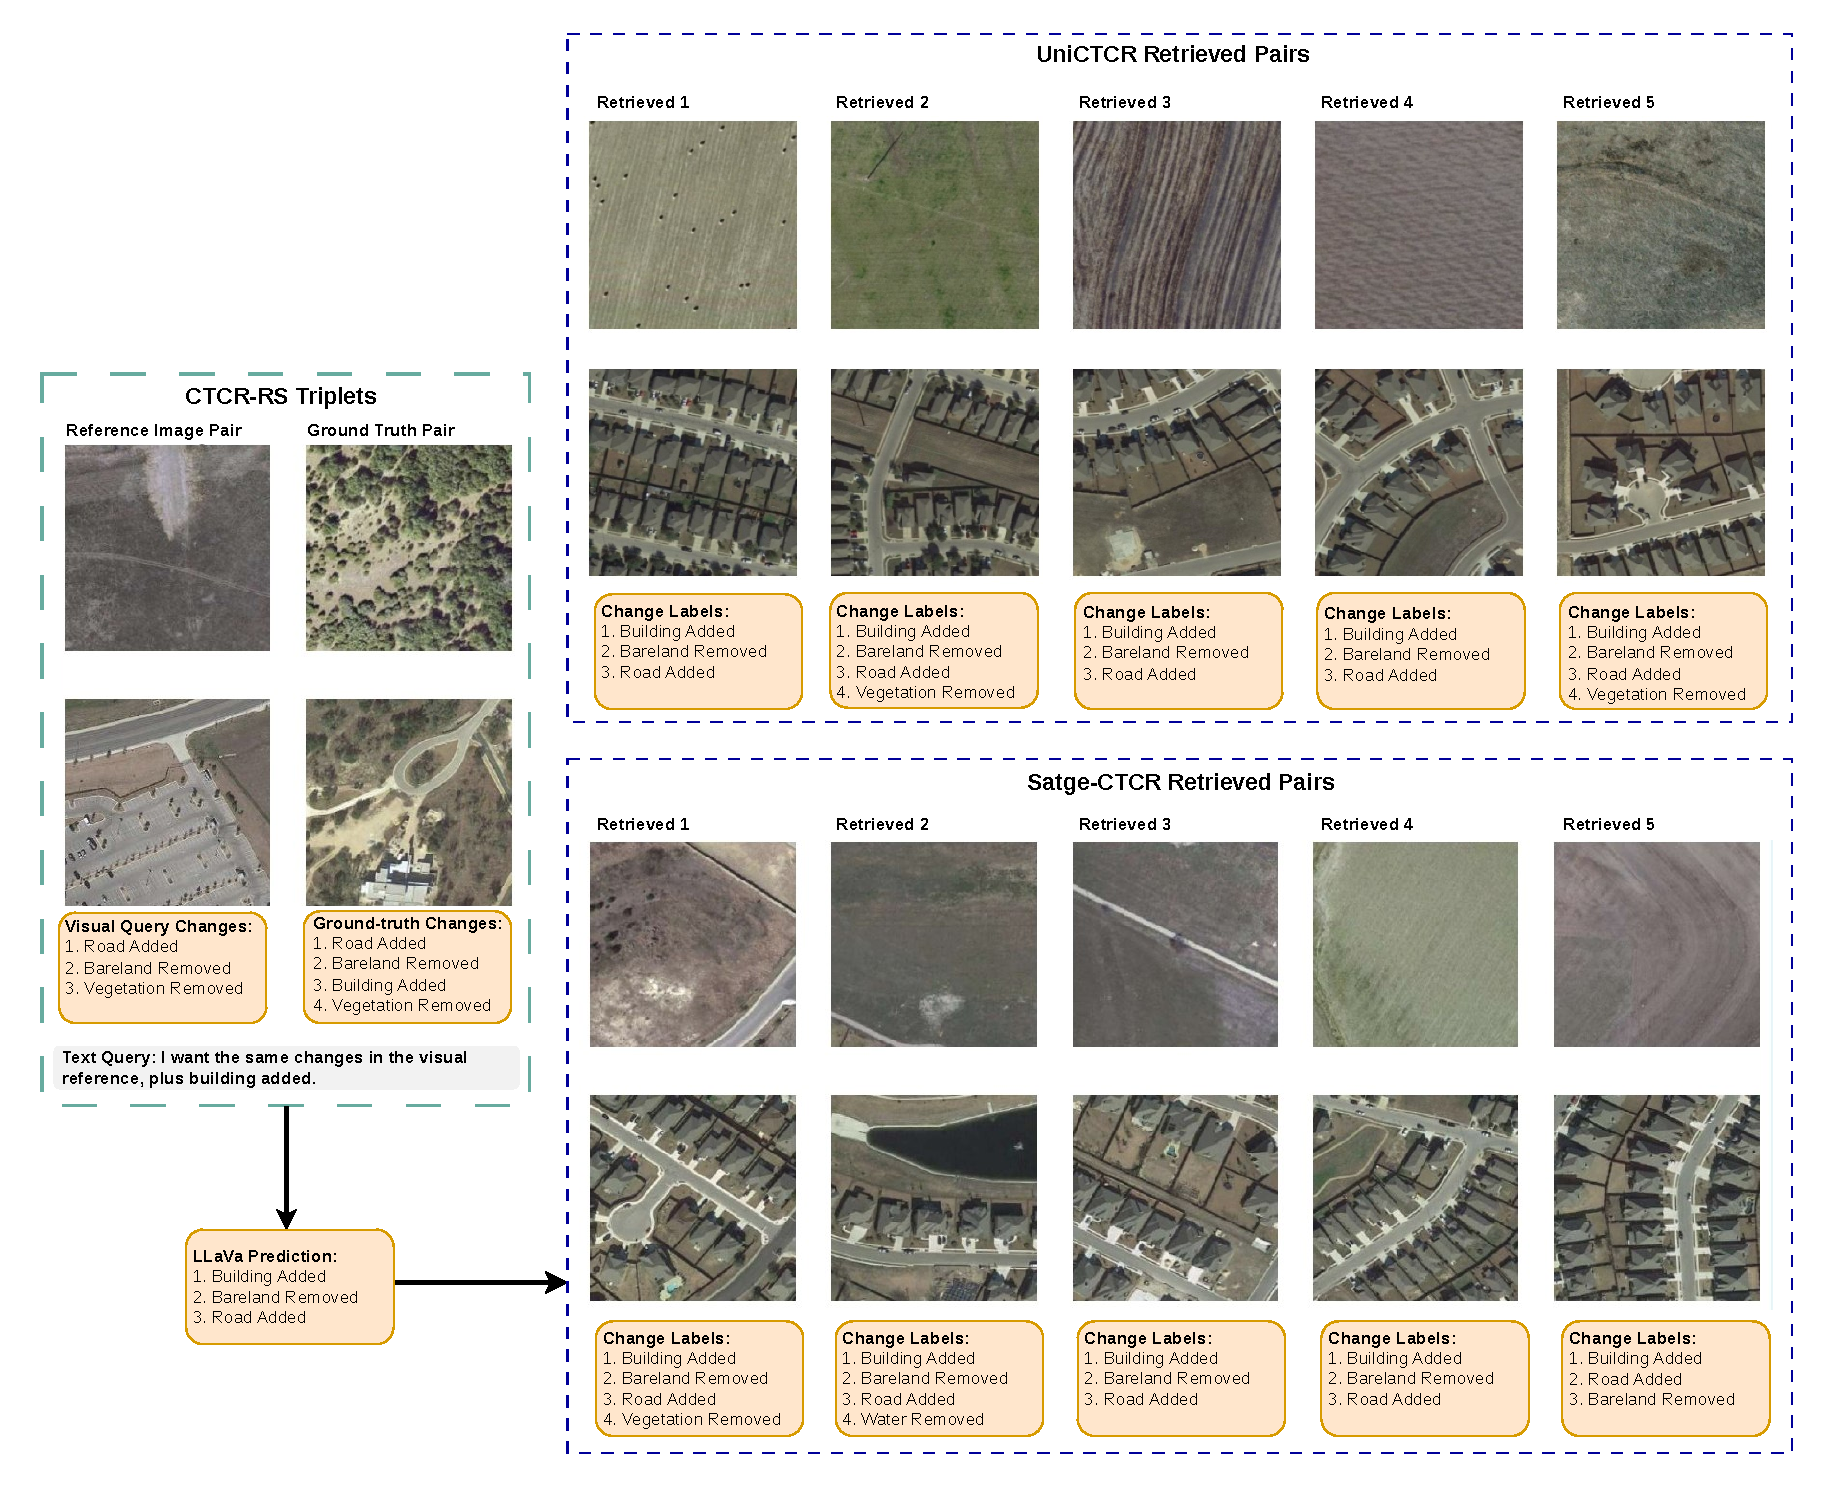
\includegraphics[width=0.85\textwidth]{images/CTCR-RS/supp-figure6.pdf}
    \caption{Impact of Stage~1 composition errors on
    retrieval. Given a reference pair with 3 visual changes
    (Road Added, Bareland Removed, Vegetation Removed) and
    a text query (Building Added), LLaVA-NeXT misses
    Vegetation Removed in its prediction. While the first
    retrieved pair is still correct (likely due to strong
    visual similarity), subsequent results lack the
    Vegetation Removed attribute.}
    \label{fig:chap6_qual_failure}
\end{figure}
 
Figure~\ref{fig:chap6_qual_success} illustrates a success
case in which StageCTCR outperforms UniCTCR due to its
explicit compositional reasoning. Figure~\ref{fig:chap6_qual_failure}
illustrates the cascading failure mode of StageCTCR: a
single missed label in Stage~1 propagates to Stage~2,
where retrieval is steered toward a slightly incorrect
semantic cluster. Despite this, the first retrieved result
is still correct, likely because of strong overall visual
similarity between matching image pairs.
 
% ============================================================
\section{Broader Impact and Ethical Considerations}
\label{sec:chap6_impact}
% ============================================================
 
\subsection{Operational Value}
\label{sec:chap6_impact_value}
 
The CTCR-RS task addresses a genuine bottleneck in
operational Earth Observation workflows. Analysts monitoring
large archives currently face an inhomogeneous query
problem: they may observe a change of interest in one
location and wish to retrieve analogous locations elsewhere
in the archive, but lack the means to specify the composed
visual-textual query efficiently. Existing text-only
retrieval requires exhaustively describing all expected
changes from scratch, a burden that grows with scene
complexity and is particularly acute for concurrent
multi-class transitions (e.g., simultaneous vegetation
removal, building construction, and road addition). The
CTCR-RS formulation reduces this burden: the reference
pair encodes the observed changes implicitly, and the
analyst needs only to specify what is additionally sought.
 
In the long term, a general-purpose CTCR-RS system could
enable applications currently infeasible at scale:
identifying all locations in a global Sentinel-2 archive
where urban expansion has co-occurred with deforestation,
surfacing candidate areas where infrastructure damage has
occurred alongside flooding during disaster response, or
tracking the spread of a specific land-cover transition
pattern across a continent over time. The current work
establishes that the task is tractable and identifies the
key technical bottlenecks; realizing this potential
requires scaling the dataset beyond the urban domain and
developing encoders capable of disentangling dense
multi-class change signatures.
 
\subsection{Dual-Use Risks}
\label{sec:chap6_impact_risks}
 
Retrieval systems capable of identifying specific land-cover
changes at scale are not without risk. The same capability
that accelerates environmental monitoring can, if misused,
enable unauthorized surveillance of sensitive
infrastructure, including military installations or
undisclosed construction activities, raising legitimate
geopolitical concerns that responsible deployment must
account for. The public availability of high-resolution EO
data (Sentinel-1/2, commercial providers) already presents
similar dual-use challenges, but a retrieval system that
can efficiently surface specific change patterns across
global archives amplifies this risk by reducing the
expertise and time required to locate areas of interest.
 
\subsection{Geographic Bias}
\label{sec:chap6_impact_bias}
 
The CTCR-RS dataset inherits the geographic biases of its
source datasets, LEVIR-CC and SECOND-CC, which predominantly
reflect developed urban environments with change patterns
characteristic of rapid urbanization in China and the
United States. As a result, the trained models may
underperform on landscape changes more common in other
regions of the world, including smallholder agricultural
expansion, informal urbanization, or primary deforestation
in the Global South. Additionally, the dataset's strong
concentration of Building Added and Bareland Removed
co-occurrences reflects a specific urbanization dynamic
that is not representative of all geographic contexts.
Prioritizing geographically diverse training distributions
and extending the curation pipeline to datasets covering
more diverse change types and regions is a critical
direction to ensure that performance gains in EO retrieval
translate equitably across global geographies.
 
% ============================================================
\section{Conclusion and Limitations}
\label{sec:chap6_conclusion}
% ============================================================
 
This chapter introduced Composed Temporal Change Retrieval
in Remote Sensing (CTCR-RS), a novel retrieval task that
enables querying EO archives through a combination of
bi-temporal reference image pairs and natural language
instructions specifying additional changes. To support this
task, the CTCR-RS dataset was constructed by normalizing
free-form change captions into a structured 14-class
geospatial ontology, yielding 30,179 compositional triplets
from two established change captioning datasets. Two
baseline architectures were proposed: UniCTCR, which
addresses the task through end-to-end latent fusion, and
StageCTCR, which decomposes the problem into explicit
semantic composition (LLaVA-NeXT via LoRA) followed by
domain-adapted retrieval (CLIP via LoRA). Results
confirm that explicit staged decomposition consistently
outperforms implicit latent fusion, with StageCTCR
surpassing UniCTCR's oracle at inference time.
 
\textbf{Limitations and Perspectives.}
Several limitations should be acknowledged.
First, the dataset is currently scoped to urban land-cover
changes derived from LEVIR-CC and SECOND-CC, limiting
the diversity of geographic contexts, change types, and
scene complexities. Extending the pipeline to multi-domain
datasets covering rural, coastal, and disaster-related
changes is the most important direction for future work.
Second, the textual queries use a fixed template (``I want
the same changes as in the reference pair, plus
[label(s)]''), which provides precision and consistency
but does not reflect the unconstrained, natural language
instructions that analysts would use in practice. Handling
free-form natural language modification queries is an
important open challenge.
Third, global vision encoders produce entangled embeddings
when four or more concurrent changes co-occur in a target
pair, causing performance to degrade severely at $>$2
visual changes. Patch-level or change-specific encoding
strategies are needed to address this limitation.
Fourth, Stage~1 composition errors cascade into Stage~2
retrieval with no mechanism for recovery. A unified model
that can jointly reason about composition and retrieval,
or an uncertainty-aware Stage~2 that discounts
low-confidence Stage~1 predictions, could mitigate this.
Fifth, the dataset construction relies on LLM extraction
with 83.5\% accuracy; the remaining 16.5\% of labels
introduce noise that is difficult to fully eliminate
without exhaustive manual annotation.
 
 


\part{Conclusion}
% ============================================================
% CHAPTER: Conclusion
% Synthesizes all six contributions, answers the five RQs
% stated in Chapter 1, identifies cross-cutting findings,
% discusses limitations and future work. Rebalanced so no
% single contribution (QUEST/Chapter 6) dominates the synthesis
% sections.
% ============================================================

\chapter{Conclusion}
\label{chap:conclusion}

\startcontents[chapters]
\printmyminitoc{
\textit{Chapter summary.} This thesis pursued five research questions on making remote sensing information accessible through natural language, across six contributions spanning single-modality RSVQA robustness and architecture, multi-modal and multi-task extensions, and a complementary retrieval paradigm. Four of the five questions receive an affirmative answer; the fourth, whether jointly training RSVQA with other tasks measurably helps, does not, at the level of aggregate metrics, a negative result that itself constitutes a contribution. This chapter synthesizes these findings, identifies patterns that only become visible across contributions rather than within any single one, and discusses this thesis's limitations and the directions it leaves open.
}
% ============================================================

\section{Summary of Contributions}
\label{sec:conclusion_summary}

This section revisits each of the thesis's five research questions in turn, stating what the corresponding contribution actually found, rather than only what it attempted.

\textbf{RQ1 (Chapter~\ref{chap:llm_augmentation}): can data-centric augmentation improve RSVQA models' robustness to linguistic variation, without sacrificing in-distribution accuracy?} Yes. Generating syntactically diverse reformulations of training questions with an instruction-tuned LLM (LLaMA-2-7B), rather than relying on back translation, improved robustness to unseen phrasings substantially: on questions reformulated by the LLM itself, the augmented model retained 81.77\% accuracy, close to its 82.98\% in-distribution accuracy, while the non-augmented model dropped to 52.16\% on the same reformulations. In-distribution accuracy was preserved (82.98\% versus 82.17\% for the non-augmented model), unlike back translation, which measurably degraded it (69.07\%), indicating that the syntactic diversity LLM-generated reformulations offer, rather than back translation's more limited variation, is what drives the generalization gain.

\textbf{RQ2 (Chapter~\ref{chap:seg_attention}): does conditioning attention on an explicit semantic segmentation prior improve RSVQA over attention computed from raw visual features alone?} Yes. Guiding attention with a frozen, multi-channel segmentation prior improved overall accuracy from 36.26\% (no attention) to 41.43\% (vanilla attention) to 45.44\% (segmentation-guided attention), a further gain of roughly 4 points from segmentation guidance specifically, on top of what attention alone already provides. This indicates that giving the model an explicit, separately trained signal for scene structure is more effective than requiring it to discover that structure from question-answering supervision alone.

\textbf{RQ3 (Chapter~\ref{chap:tammi}): how can RSVQA be extended to jointly exploit multiple sensing modalities acquired at different spatial resolutions?} By treating the resolution mismatch between modalities as a deliberate, user-configurable design choice rather than a limitation to be resolved architecturally: TAMMI extracts multispectral and SAR context at an independently configurable spatial extent around each VHR patch, and MM-RSVQA fuses the resulting three-modality representation with the question through trainable attention. Multimodal fusion improved average accuracy from 61.94\% (VHR-only) to 65.56\% (all three modalities), with the largest gains concentrated in questions requiring context beyond what a single VHR patch's extent can contain, such as urban classification (+24.6 points) and administrative department (+9.2 points). This benefit is not solely a matter of broader spatial context, however: SAR's contribution peaked specifically on land cover classification (74.89\%, the highest accuracy across every configuration tested, including the full three-modality model), consistent with SAR's physical sensitivity to surface roughness and dielectric properties rather than with the additional spatial extent it provides. Modalities can therefore be complementary along two distinct axes, the spatial context they cover and the physical property they are sensitive to, and both, not context alone, account for multimodal fusion's benefit here.

\textbf{RQ4 (Chapter~\ref{chap:multitask}): does training RSVQA jointly with captioning and self-supervised image reconstruction measurably improve either task?} No, not at the level of aggregate metrics. Single-task training matched or outperformed every multi-task configuration on both captioning and VQA. A closer look, however, qualified this result rather than simply confirming it: a modality-specific weakness in the multispectral reconstruction plausibly diluted the aggregate reconstruction signal, and a qualitative counter-example showed the full multi-task model succeeding on a specific question where the single-task baseline failed, meaning the aggregate result does not rule out category-specific synergy, even though it does not establish it either.

\textbf{RQ5 (Chapter~\ref{chap:ctcr}): can a composed query, combining a visual reference and a textual description, support retrieval of temporal change patterns in Earth Observation archives?} Yes. Composed Temporal Change Retrieval, introduced as a task in this thesis, is addressed effectively by decomposing the composed query into its reference and textual components before fusion (StageCTCR), which outperformed a direct end-to-end fusion of the two (UniCTCR). This advantage is not attributable to the staged decomposition alone: StageCTCR also leverages a pretrained vision-language model that UniCTCR's more directly fused architecture does not benefit from in the same way, so the two factors are confounded in this comparison rather than isolated. What can be said is that staged decomposition combined with pretrained vision-language representations outperformed direct end-to-end fusion; disentangling how much each factor individually contributes is left to future work.

\section{Cross-Cutting Findings}
\label{sec:conclusion_crosscutting}

Considered individually, each contribution answers the research question it was designed to address. Considered together, three patterns emerge that are not visible from any single chapter alone.

\textbf{RSVQA's remaining weaknesses are distributed across several independent levers, not concentrated in one.} Chapters~\ref{chap:llm_augmentation} and~\ref{chap:seg_attention} improve RSVQA from two different angles, data-centric augmentation and architectural attention design, without either depending on the other; Chapter~\ref{chap:tammi} then adds a third, largely orthogonal lever, showing that modality choice itself, independent of both linguistic diversity and attention design, measurably changes what a model can answer, and does so through two distinct mechanisms, spatial context and sensor-specific physical sensitivity, rather than one. Taken together, these three contributions suggest that RSVQA's remaining gaps are not a single bottleneck a lone intervention could close, but several largely independent axes, each requiring its own targeted solution.

\textbf{Reconciling heterogeneous visual signals is a recurring design problem, addressed differently each time it recurs.} Chapter~\ref{chap:seg_attention} reconciles a question with a segmentation prior at the same spatial resolution; Chapter~\ref{chap:tammi} reconciles three modalities at three different resolutions by making that mismatch a configurable dataset property rather than an architectural constraint; Chapter~\ref{chap:multitask} reconciles those same modalities with two additional training objectives within one architecture; and Chapter~\ref{chap:ctcr} reconciles a visual reference with a textual description of change within a composed query. No single solution recurs across these four instances, an attention mechanism, a dataset design choice, a shared multi-objective architecture, and a staged retrieval pipeline, respectively, suggesting that reconciling heterogeneous visual and textual signals in remote sensing is not a problem this thesis's contributions solve once and reuse, but one that resurfaces in a different form at each new combination of modality, task, and resolution.

\textbf{Assumed multi-task synergy does not straightforwardly hold.} Chapter~\ref{chap:relatedworks} noted that RS-LLaVA's own reported results show single-task fine-tuning outperforming joint training on both captioning and VQA metrics, an isolated observation drawn from prior work rather than a result this thesis produced itself. Chapter~\ref{chap:multitask} then measured the same question directly, on a different dataset, a different architecture, and a different task combination, and found the same pattern. Two independent measurements of the same negative result is a stronger basis for caution than either alone, and should be treated as reason to test rather than assume similar synergy claims elsewhere, including Chapter~\ref{chap:ctcr}'s own finding, where the respective contributions of staged decomposition and pretrained representations were deliberately not assumed but left as an open, explicitly confounded question rather than a settled one.

\section{Limitations}
\label{sec:conclusion_limitations}

Beyond the limitations already discussed within each individual chapter, three limitations apply across this thesis as a whole.

\textbf{Geographic and sensor scope.} The datasets introduced in this thesis, TAMMI and its extensions, are constructed over Metropolitan France specifically, combining VHR, Sentinel-2, and Sentinel-1 imagery. Whether the findings in Chapters~\ref{chap:tammi} and~\ref{chap:multitask} generalize to other geographic regions, land cover distributions, or sensor combinations was not tested, and is not something this thesis's results can be assumed to predict.

\textbf{Scale.} Each contribution in this thesis evaluates one architecture, at a scale consistent with academic compute constraints, rather than a systematic sweep across model or data scale. Whether the specific quantitative findings reported throughout this thesis, including RQ4's negative result on multi-task synergy, hold as model and data scale increase remains untested.

\textbf{Confounded comparisons left undisentangled.} Two contributions identify an effect without fully isolating its cause. In Chapter~\ref{chap:multitask}, the multispectral reconstruction weakness was localized to a specific, patch-internal artifact but not conclusively confirmed, and the per-question-type breakdown needed to determine whether multi-task synergy might hold for specific question categories despite the aggregate negative result was left incomplete. In Chapter~\ref{chap:ctcr}, StageCTCR's advantage over UniCTCR was shown to depend on both staged decomposition and pretrained vision-language representations jointly, without disentangling how much each factor individually contributes. Both cases identify a real effect while leaving its precise mechanism for future work to establish.

\section{Future Work}
\label{sec:conclusion_future}

The limitations above point directly to concrete extensions of this work, alongside broader directions this thesis's findings motivate but does not itself pursue.

Within individual chapters, two disentangling studies would directly extend this thesis's confounded findings. Completing the per-question-type breakdown for Chapter~\ref{chap:multitask}'s four training configurations would test whether the aggregate absence of multi-task synergy masks category-specific effects of the kind its qualitative example suggests, or holds uniformly; addressing the multispectral reconstruction weakness identified in the same chapter, most plausibly by replacing the affected decoder's index-based unpooling with a learned upsampling stage, would clarify whether it was a genuine contributor to reconstruction's limited measured benefit. Separately, evaluating an end-to-end CTCR-RS architecture that also benefits from pretrained vision-language representations would isolate how much of StageCTCR's advantage over UniCTCR, reported in Chapter~\ref{chap:ctcr}, is attributable to staged decomposition specifically, rather than to the two factors' current confound.

More broadly, this thesis's two directions, RSVQA and CTCR-RS's composed retrieval, were developed as complementary but separate paradigms. Whether the multi-modal, multi-resolution representations developed for RSVQA in Chapters~\ref{chap:tammi} and~\ref{chap:multitask} could support composed retrieval directly, or whether retrieval requires representations shaped differently from the ones question answering benefits from, is an open question this thesis's separation of the two paradigms does not itself answer. Finally, extending the datasets introduced in this thesis beyond Metropolitan France for TAMMI, and to further change captioning datasets for CTCR-RS, would test how far the specific findings reported here actually generalize, rather than assuming they do.

\section{Closing Remarks}
\label{sec:conclusion_closing}

This thesis set out to make remote sensing information more accessible through natural language, along two directions: answering questions about a known location, and retrieving locations that match a description. Across its five research questions, targeted interventions, data-centric augmentation, segmentation-guided attention, multi-modal fusion, and composed retrieval, each measurably improved on the specific gap they were designed to close, though rarely through a single mechanism: modality choice helped through two distinct physical properties rather than one, and composed retrieval's own gain was shown to rest on two confounded factors rather than a single clean cause. The one question that did not confirm what it set out to test, whether jointly training RSVQA with other tasks helps, is not a shortfall among these results but one of the more informative ones: an assumption common enough in the field to motivate real datasets and real model designs was tested directly, on new data and a new architecture, and did not hold, echoing an independent finding already present in the literature. Taken together, these six contributions leave remote sensing information more accessible through language than this thesis found it, and leave a clearer sense than before of which assumptions in that pursuit still need testing, rather than taking for granted.


\printbibliography
\addcontentsline{toc}{chapter}{Bibliographie}

\end{document}
